\documentclass[]{htwg-report}

% Use german umlaute
\usepackage{german,ngerman}
\usepackage[T1]{fontenc}
\usepackage[utf8]{inputenc}
\usepackage[ngerman]{babel}
\usepackage[autostyle=true,german=quotes]{csquotes}

%\usepackage[table]{xcolor}\usepackage{float}
%\usepackage{xcolor,colortbl}

\usepackage{graphicx}
\usepackage[noend]{algpseudocode}
\usepackage{algorithm}
%\usepackage{algorithmic}
%\usepackage{algpseudocode}
\usepackage{booktabs} 
\usepackage{array,hhline} 
\usepackage{mathtools}
\usepackage{hyperref}
\usepackage{tabularx}
\usepackage{tabulary}
\usepackage[official]{eurosym}
\usepackage{hyperref}
\RequirePackage[ngerman=ngerman-x-latest]{hyphsubst}
\usepackage{microtype}% verbesserter Randausgleich
\usepackage{acronym}
%\usepackage[german]{nomencl}
%\makenomenclature

\algnewcommand\algorithmicforeach{\textbf{for each}}
\algdef{S}[FOR]{ForEach}[1]{\algorithmicforeach\ #1\ \algorithmicdo}


\addbibresource{./bib/report.bib}

\begin{document}

\renewcommand{\figurename}{Abbildung}
\renewcommand{\tablename}{Tabelle}
\renewcommand{\contentsname}{Inhaltsverzeichnis}
\renewcommand{\listfigurename}{Abbildungsverzeichnis}
\renewcommand{\listtablename}{Tabellenverzeichnis}

%% Use Roman numerals fotr he page numbers of the title pages and table of
%% contents.
\frontmatter

%% 'reporttype' add background elements to the cover / front page
%% possible values are:
%% bachelor	--> B S C
%% master	--> M S C
%% other		--> none
\reporttype{master}
\reporttypetext{Master Thesis} 

\title[Analyse der Anwendbarkeit und Erweiterungen eines Segment-basierten SLAM-Algorithmus auf Indoor-Umgebungen mit einer RGB-D Kamera]{Analyse der Anwendbarkeit und Erweiterungen eines Segment-basierten SLAM-Algorithmus auf Indoor-Umgebungen mit einer RGB-D Kamera}

\author{Miriam Schmelzer}
\studentnumber{123456}
\studentemail{Miriam.Schmelzer@htwg.de}
\newcommand{\verfasserA}{Miriam Schmelzer}
\newcommand{\verfasserB}{Florian Kopp}
\newcommand{\thema}{Analyse der Anwendbarkeit und Erweiterungen eines Segment-basierten SLAM-Algorithmus auf Indoor-Umgebungen mit einer RGB-D Kamera}
\newcommand{\dobA}{16.08.1994}
\newcommand{\birthplaceA}{Bochum}
\newcommand{\dobB}{22.04.1990}
\newcommand{\birthplaceB}{Böblingen}
\newcommand{\hoschschule}{Hochschule Konstanz (HTWG)}
\newcommand{\institut}{HTWG Konstanz, Labor für mobile Robotik}
\newcommand{\prueferA}{Prof. Dr. Oliver Bittel}
\newcommand{\prueferB}{Dipl.-Inf.-Wiss. Jürgen Keppler}
\newcommand{\ausgabedatum}{01.09.2019}
\newcommand{\abgabedatum}{29.05.2020}
\newcommand{\type}{Master}
\newcommand{\typeshortcut}{M}
\newcommand{\studiengangA}{Master Informatik}
\newcommand{\studiengangB}{Elektrische Systeme}
\newcommand{\strasseA}{Muntpratstr. 9}
\newcommand{\wohnortA}{78462 Konstanz}
\newcommand{\strasseB}{Josef-Haydn-Weg 6}
\newcommand{\wohnortB}{71032 Böblingen}
\newcommand{\schlagworte}{ROS, Segmentierung, SLAM, RGB-D Kamera}

\doclocation{Konstanz}
\docdate{25 Mai 2020}
%          
%% Include an optional title page.
\begin{titlepage}
\newgeometry{hscale=0.81,vscale=0.8}

\AddToShipoutPicture*{\BackgroundImgTitelPage}

\vspace*{\bigskipamount}


%% Print the title in htwg-teal.
{\makeatletter
\fboxsep=0pt
\colorbox{htwg-white}{\begin{minipage}[t]{145mm}
    \begin{flushleft}
        %% Print Report Type Text
        \color{htwg-teal}{\Large \@report@typetext}
        \\
        %% Print Report Title
        \color{htwg-teal}\Large \textbf{\@title}
    \end{flushleft}
\end{minipage}}
\makeatother}

\bigskip
\bigskip

{
\setlength{\parskip}{0.5cm}
\begin{center}
	\textbf{zur Erlangung des akademischen Grades}
	
	\textbf{\Large \type\ of Science (\typeshortcut. Sc.)}
	
		\textbf{bzw.}

	\textbf{\Large \type\ of Engineering (\typeshortcut.Eng.))}

	\textbf{an der}
	
	\textsf{\huge Hochschule Konstanz}\\
	{\small Technik, Wirtschaft und Gestaltung}
	
    \textsf{\Large Fakultät Informatik} \\
	Studiengang \studiengangA
	
\end{center}
}

\bigskip
\bigskip
\bigskip

\begin{center}
	\begingroup
	\renewcommand*{\arraystretch}{1}
	\rowcolors{2}{white}{white}
	{\makeatletter
		\begin{tabular}{lll}
			\type kandidaten: & \verfasserA \\
							& \strasseA \\
							& \wohnortA \\ \\

							& \verfasserB \\
							& \strasseB \\
							& \wohnortB \\ \\ 					
						
	
			1. Prüfer: & \prueferA \\
			2. Prüfer: & \prueferB \\ \\ \\ \\
			
			Ausgabedatum: & \ausgabedatum \\
			Abgabedatum: & \abgabedatum
		\end{tabular}
		\makeatother}
	\endgroup
\end{center}


%% reset page margins
\newgeometry{hscale=0.7,vscale=0.8}
\end{titlepage}



\begin{titlepage}
\newgeometry{hscale=0.81,vscale=0.8}

\AddToShipoutPicture*{\BackgroundImgTitelPage}

\vspace*{\bigskipamount}


%% Print the title in htwg-teal.
{\makeatletter
\fboxsep=0pt
\colorbox{htwg-white}{\begin{minipage}[t]{145mm}
    \begin{flushleft}
        %% Print Report Type Text
        \color{htwg-teal}\Large {\@report@typetext}
        \\
        %% Print Report Title
        \color{htwg-teal}\Large \textbf{\@title}
    \end{flushleft}
\end{minipage}}
\makeatother}

\bigskip
\bigskip

{
\setlength{\parskip}{0.5cm}
\begin{center}
	\textbf{zur Erlangung des akademischen Grades}
	
	\textbf{\Large \type\ of Engineering (\typeshortcut. Eng.)}
	
	\textbf{an der}
	
	\textsf{\huge Hochschule Konstanz}\\
	{\small Technik, Wirtschaft und Gestaltung}
	
    \textsf{\Large Fakultät Elektrotechnik und Informationstechnik} \\
	Studiengang \studiengangB
	
\end{center}
}

\bigskip
\bigskip
\bigskip

\begin{center}
	\begingroup
	\renewcommand*{\arraystretch}{1}
	\rowcolors{2}{white}{white}
	{\makeatletter
		\begin{tabular}{lll}
			\type kandidaten: & \verfasserB \\
							& \strasseB \\
							& \wohnortB \\ \\ \\ \\
	
			1. Prüfer: & \prueferA \\
			2. Prüfer: & \prueferB \\ \\ \\ \\
			
			Ausgabedatum: & \ausgabedatum \\
			Abgabedatum: & \abgabedatum
		\end{tabular}
		\makeatother}
	\endgroup
\end{center}


%% reset page margins
\newgeometry{hscale=0.7,vscale=0.8}
\end{titlepage}




\chapter*{Abstract}
\setheader{Abstract}


\begin{center}
	\begingroup
	\renewcommand*{\arraystretch}{1}
	\rowcolors{2}{white}{white}
	{\makeatletter	
		\begin{tabular}{p{3.2cm}p{9.6cm}}
			Thema: & \thema \\
			& \\
			\type kandidaten: & \verfasserA \\
							  & \verfasserB \\
			& \\
			Betreuung: & \hoschschule \newline \prueferA \newline \prueferB \\
			& \\
			Abgabedatum: & \abgabedatum \\
			& \\
			Schlagworte: & \schlagworte \\
			& \\
		\end{tabular}
	
	\makeatother}
	\endgroup
\end{center}

\bigskip

\noindent

Im Rahmen dieser Masterarbeit wird die Anwendbarkeit des SegMap-Algorithmus auf indoor-Umgebungen analysiert und entsprechend angepasst. Dieser ist auf die Verarbeitung von LiDAR-Daten ausgelegt und wird auf die Verarbeitung der Daten einer RGB-D Kamera angepasst. Der Algorithmus basiert auf einer Umgebungserkennung anhand von Segmenten. Die verwendeten Segmentierungsmethoden werden auf eine Verarbeitung von Farbinformationen erweitert. Für die Validierung der Anwendbarkeit des Algorithmus werden diverse indoor-Datensätze mit einer RGB-D Kamera erstellt und hierfür eine Vorrichtung zur Aufzeichnung der Odometrieinformation gebaut. Der Deep-Learning-basierte Segmentdeskriptor wird mit diesen Datensätzen trainiert und die Ergebnisse ausgewertet. 
%\input{extended_abstract}
\chapter*{Ehrenwörtliche Erklärung}
\setheader{Ehrenwörtliche Erklärung}


Hiermit erkläre ich
\textit{\verfasserA, geboren am \dobA\ in \birthplaceA}, dass ich\\

\begin{tabular}{lp{12cm}}
\rowcolor{white} (1) & meine MASTERARBEIT mit dem Titel \\[1em]
\rowcolor{white} & \textbf{\thema} \\[1em]
\rowcolor{white} & in Form einer Gruppenarbeit mit Florian Kopp an der \hoschschule\ unter Anleitung von \prueferA\ selbständig und ohne fremde Hilfe angefertigt und keine anderen als die angeführten Hilfen benutzt habe;\\[1em]
\rowcolor{white} (2) & die Übernahme wörtlicher Zitate, von Tabellen, Zeichnungen, Bildern und
Programmen aus der Literatur oder anderen Quellen (Internet) sowie die Verwendung
der Gedanken anderer Autoren an den entsprechenden Stellen innerhalb der Arbeit
gekennzeichnet habe.\\
\rowcolor{white} (3) & dass die eingereichten Abgabe-Exemplare in Papierform und im PDF-Format vollständig übereinstimmen.\\

\end{tabular}

\vspace*{0.5cm}

\noindent
Ich bin mir bewusst, dass eine falsche Erklärung rechtliche Folgen haben wird.\\

\vspace*{0.5cm}

\noindent
Konstanz, \abgabedatum \hfill \begin{tabular}{c} \\ \rowcolor{white} \rule{5cm}{1pt} \\ (Miriam Schmelzer)\end{tabular}

\chapter*{Ehrenwörtliche Erklärung}
\setheader{Ehrenwörtliche Erklärung}


Hiermit erkläre ich
\textit{\verfasserB, geboren am \dobB\ in \birthplaceB}, dass ich\\

\begin{tabular}{lp{12cm}}
\rowcolor{white} (1) & meine MASTERARBEIT mit dem Titel \\[1em]
\rowcolor{white} & \textbf{\thema} \\[1em]
\rowcolor{white} & in Form einer Gruppenarbeit mit Miriam Schmelzer an der \hoschschule\ unter Anleitung von \prueferA\ selbständig und ohne fremde Hilfe angefertigt und keine anderen als die angeführten Hilfen benutzt habe;\\[1em]
\rowcolor{white} (2) & die Übernahme wörtlicher Zitate, von Tabellen, Zeichnungen, Bildern und
Programmen aus der Literatur oder anderen Quellen (Internet) sowie die Verwendung
der Gedanken anderer Autoren an den entsprechenden Stellen innerhalb der Arbeit
gekennzeichnet habe.\\
\rowcolor{white} (3) & dass die eingereichten Abgabe-Exemplare in Papierform und im PDF-Format vollständig übereinstimmen.\\

\end{tabular}

\vspace*{0.5cm}

\noindent
Ich bin mir bewusst, dass eine falsche Erklärung rechtliche Folgen haben wird.\\

\vspace*{0.5cm}

\noindent
Konstanz, \abgabedatum \hfill \begin{tabular}{c} \\ \rowcolor{white} \rule{5cm}{1pt} \\ (Florian Kopp)\end{tabular}


\tableofcontents

\listoffigures

\listoftables

%\newpage
%\section*{Abkürzungsverzeichnis}
%\begin{acronym}
%\acro{slam}[SLAM]{Simultaneous Localization and Mapping}
%\end{acronym}

%\printnomenclature
%\printacronyms
%\include{abkuerzung_acroListe}
%\input{abkuerzungen}

%% Use Arabic numerals for the page numbers of the chapters.
\mainmatter

%% \input{chapter-1}

\chapter[Einleitung (Schmelzer)]{Einleitung}

%RGBD im Kommen
%Sensorik günstiger
%mobile Roboter

Mobile Roboter sind in den letzten Jahren immer weiter in den Fokus der Entwicklung gerückt. Sowohl im industriellen als auch im privaten Umfeld können sie ein breit gefächertes Spektrum von Aufgaben übernehmen. Weitere Einsatzgebiete sind in der Agrarwirtschaft, in Such- und Rettungsmissionen sowie im Katastrophenschutz und im Militär. Gerade in der Industrie können durch den Einsatz mobiler Roboter die Effizienz gesteigert und Arbeitsplätze gespart werden. Langfristig werden somit Kosten minimiert und die Sicherheit des Arbeitsumfelds verbessert. Außerdem eignen sich mobile Roboter besonders für den Einsatz in gefährlichem und unwegsamen Gelände, da Aufgaben, wie beispielsweise eine Bombenentschärfung, erledigt werden können ohne Menschen in Gefahr zu bringen.   

Mobile Roboter zeichnen sich dadurch aus, dass sie sich in ihrer Umgebung bewegen können und nicht, wie stationäre Roboter, an einen Ort gebunden sind. Die Abbildungen \ref{fig:stationär} bis \ref{fig:logistik} zeigen Beispiele verschiedener Roboter. In Abbildung \ref{fig:stationär} ist ein typischer stationärer Industrieroboter in Form eines Greifarms abgebildet. Auf den anderen Abbildungen sind verschiedene mobile Roboter dargestellt. Abbildung \ref{fig:staub} zeigt einen Staubsaugerroboter, Abbildung \ref{fig:feuer} einen Roboter für Einsätze im Katastrophenschutz und  Abbildung \ref{fig:logistik} einen Roboter von Boston Dynamics bei einer Logistik-Anwendung. 

\afterpage{
\begin{figure}[htb]
	\centering
	\begin{minipage}[t]{0.15\linewidth}
		\centering
		\includegraphics[width = \linewidth]{Bilder/stat_rob.png}
		\caption[Beispiel eines stationären Roboters in Form eines Greifarms]{Beispiel eines stationären Roboters in Form eines Greifarms\footnotemark}
		\label{fig:stationär}
	\end{minipage}
	\hfill
	\begin{minipage}[t]{0.2\linewidth}
		\centering
		\includegraphics[width = \linewidth]{Bilder/staubsaugerroboter.png}
		%\caption{Beispiel eines mobilen Staubsaugerroboters}
		\caption[Beispiel eines mobilen Staubsaugerroboters]{Beispiel eines mobilen Staubsaugerroboters\footnotemark}
		\label{fig:staub}
	\end{minipage}
	\hfill
	\begin{minipage}[t]{0.25\linewidth}
		\centering
		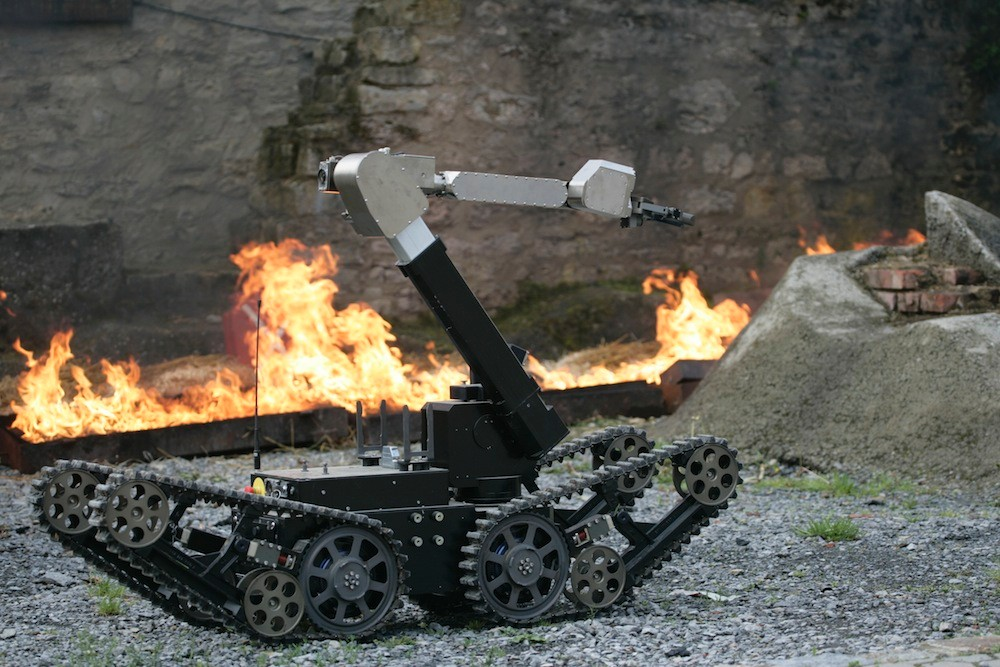
\includegraphics[width = \linewidth]{Bilder/feuerwehr.jpg}
		%\caption{Beispiel eines mobilen Roboters zum Einsatz im Katastrophenschutz}
		\caption[Beispiel eines mobilen Roboters zum Einsatz im Katastrophenschutz]{Beispiel eines mobilen Roboters zum Einsatz im Katastrophenschutz\footnotemark}
		\label{fig:feuer}
	\end{minipage}
	\hfill
	\begin{minipage}[t]{0.3\linewidth}
		\centering
		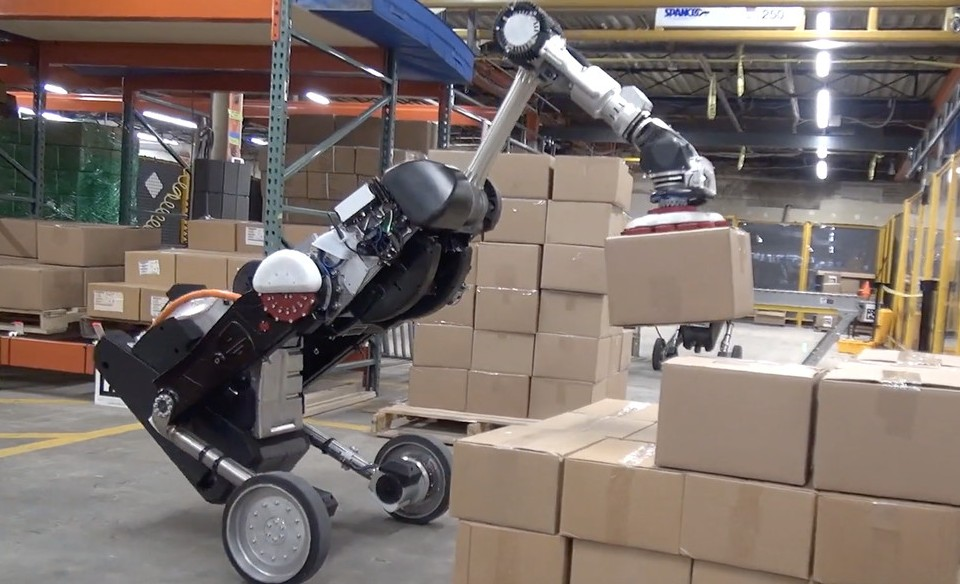
\includegraphics[width = \linewidth]{Bilder/industrie.jpg}
		%\caption{Beispiel eines mobilen Roboters bei einer Logistik-Anwendung}
		\caption[Beispiel eines mobilen Roboters bei einer Logistik-Anwendung]{Beispiel eines mobilen Roboters bei einer Logistik-Anwendung\footnotemark}
		\label{fig:logistik}
	\end{minipage}
\end{figure}
\addtocounter{footnote}{-3}
\footnotetext{\url{https://de.cleanpng.com/png-t0sbpe/}}
\stepcounter{footnote}
\footnotetext{\url{https://www.philips.de/c-m-ho/staubsauger/staubsauger-roboter/robotics}}
\stepcounter{footnote}
\footnotetext{\url{https://idw-online.de/de/news520138}}
\stepcounter{footnote}
\footnotetext{\url{https://www.technologyreview.com/s/613260/boston-dynamics-kinema-acquisition/}}
}

Da mobile Roboter nicht ortsgebunden sind, benötigen sie viel Sensorik und Rechenleistung, um ihre sich ständig ändernde Umgebung wahrzunehmen und verarbeiten zu können. Immer günstiger werdende Sensorik und Hardware sowie die steigende Leistungsfähigkeit bei gleichzeitig kleiner werdender Baugröße treiben die schnelle \linebreak Entwicklung mobiler Roboter voran. Außerdem ermöglichen Entwicklungen in anderen Forschungsgebieten, wie beispielsweise der künstlichen Intelligenz, neue Lösungsansätze für bestehende Probleme und erschließen neue Anwendungsfelder. 

Es gibt viele verschiedene Arten von mobilen Robotern. Sie unterscheiden sich anhand ihrer Konstruktion und Erscheinungsform, die sowohl an ihre Aufgaben als auch an die Umgebung, in der sie diese verrichten sollen, angepasst ist. Die Abbildungen \ref{fig:zipline} bis \ref{fig:cat} zeigen verschiedene mobile Roboter in unterschiedlichen Umgebungen. Sie können sowohl an Land, als auch in der Luft sowie auf und unter Wasser eingesetzt werden. Abbildung \ref{fig:zipline} zeigt eine Drohne, die in Afrika eingesetzt wird, um möglichst schnell Medikamente, Impfstoffe und Blutspenden an abgelegene Krankenhäuser auszuliefern. Auf Abbildung \ref{fig:spot} ist der Spot Mini von Boston Dynamics abgebildet, der auch Hindernisse überwinden kann. Das Institut für Systemdynamik der HTWG entwickelt mit dem Projekt CaRoLIME einen autonomen Wasserroboter, der autonom in unbekannten Umgebungen navigieren und arbeiten kann. Dieser ist auf Abbildung \ref{fig:cat} abgebildet. 

\afterpage{
\begin{figure}[htb]
	\centering
	\begin{minipage}[t]{0.3\linewidth}
		\centering
		\includegraphics[width = \linewidth]{Bilder/ghana.png}
		\caption[Ein unbemanntes Luftfahrzeug als Beispiel eines mobilen Roboters]{Ein unbemanntes Luftfahrzeug von Zipline zur Auslieferung von Medikamenten\footnotemark}
		\label{fig:zipline}
		%\footnotetext{\url{https://www.gemeinsam-fuer-afrika.de/ghana-medikamente-drohne/}}
	\end{minipage}
	\hfill
	\begin{minipage}[t]{0.3\linewidth}
		\centering
		\includegraphics[width = \linewidth]{Bilder/bostondynamics-spotmini.png}
		%\caption{Spot Mini von Boston Dynamics}
		\caption[Spot Mini von Boston Dynamics]{Spot Mini von Boston Dynamics\footnotemark}
		\label{fig:spot}
		%\footnotetext{\url{https://www.wevolver.com/wevolver.staff/spot.mini/}}
	\end{minipage}
	\hfill
	\begin{minipage}[t]{0.3\linewidth}
		\centering
		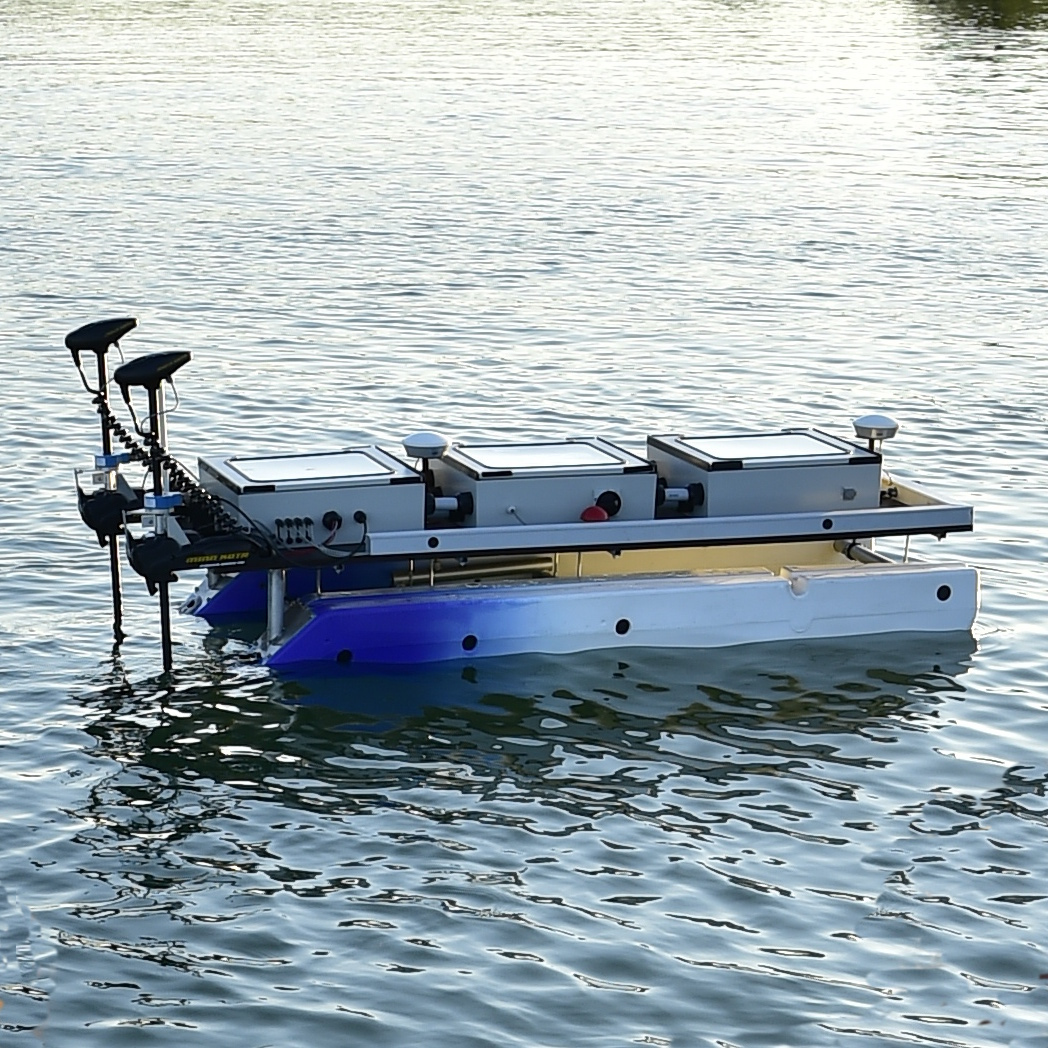
\includegraphics[width = \linewidth]{Bilder/CaRoLime.jpg}
		%\caption{Projekt CaRoLime des Instituts für Systemdynamik der HTWG}
		\caption[Projekt CaRoLime des Instituts für Systemdynamik der HTWG]{Projekt Ca\-Ro\-Lime des Instituts für Systemdynamik der HTWG\footnotemark}
		\label{fig:cat}
		%\footnotetext{\url{https://www.htwg-konstanz.de/forschung-und-transfer/institute-und-labore/isd/regelungstechnik/allgemein/}}
	\end{minipage}
\end{figure}
\addtocounter{footnote}{-2}
\footnotetext{\url{https://www.gemeinsam-fuer-afrika.de/ghana-medikamente-drohne/}}
\stepcounter{footnote}
\footnotetext{\url{https://www.wevolver.com/wevolver.staff/spot.mini/}}
\stepcounter{footnote}
\footnotetext{\url{https://www.htwg-konstanz.de/forschung-und-transfer/institute-und-labore/isd/regelungstechnik/allgemein/}}
}

%Die verschiedenen Konstruktionen und Erscheinungsformen sind sowohl an ihre Aufgaben als auch an die Umgebung, in der sie diese verrichten sollen, angepasst. 

Unabhängig von ihrem mit unter sehr verschiedenen Aufbau, Erscheinungsformen und Anforderungsprofil, haben alle mobilen Roboter gemeinsam, dass sie sich im Idealfall autonom auch in unbekannten Umgebungen zuverlässig orientieren müssen. Dafür müssen sie in der Lage sein eine genaue Karte der Umgebung zu erstellen sowie sich gleichzeitig in dieser zuverlässig zu lokalisieren. Dieses Verfahren wird %\ac{slam} 
Simultaneous Localization and Mapping (SLAM) genannt. 

\section[Motivation (Schmelzer)]{Motivation}

Bei SLAM-Verfahren basiert die Lokalisierung in der Karte auf dem Wiedererkennen schon einmal besuchter und kartierter Orte. Dies wird Place Recognition oder auch Loop Closure genannt. Hierfür gibt es verschiedene Ansätze, die sich in erster Li\-nie darin unterscheiden, wie der Roboter seine Umgebung wahrnimmt und verarbeitet. Häufig werden als Sensoren zur Umgebungswahrnehmung Kameras,LiDARs, Ultraschallsensoren oder Radars eingesetzt. 

Bildbasierte SLAM-Verfahren leiden häufig unter Fehleranfälligkeit bei Beleuchtungs- oder Blickwinkeländerungen. LiDAR-Sensoren liefern Entfernungsmessungen in Form von Punktwolken mit Hilfe derer die Umgebung in hoher Auflösung anhand ihrer Strukturen wahrgenommen wird. Daher wird die Qualität LiDAR-basierter SLAM-Verfahren nicht durch Beleuchtungsänderungen beeinflusst. Außerdem sind die Auswirkungen von Blickwinkeländerungen geringer.  

Um Loop Closures erfolgreich erkennen zu können, müssen  verschiedenen Orte eindeutig unterscheidbar beschrieben werden. Hierfür gibt es verschiedene Ansätze. Ein häufig verwendeter Ansatz ist das Wiedererkennen markanter Punkte in den Punkt\-wol\-ken, sogenannte Keypoints. Diese sind jedoch nicht immer eindeutig unterscheidbar und die Wiedererkennung ist abhängig vom Blickwinkel. Ein weiterer Ansatz ist das Matchen von Objekten, die aus den Punktwolken extrahiert werden. Diese Art der Umgebungswahrnehmung ist ähnlicher zur menschlichen Wahrnehmung. Außerdem können Karten auf Basis von Objekten besser Situationen repräsentieren, in denen statische Objekte dynamisch werden. 

Ein Nachteil bei der Repräsentation der Umgebung anhand von Objekten ist, dass sich reale Umgebungen häufig nicht ausschließlich aus tatsächlichen Objekten, die eindeutig unterscheidbar sind, zusammensetzen. Außerdem wird ein perfekter Objektsegmentierungsalgorithmus benötigt. 

Einen anderen Ansatz verwendet der SegMap-Algorithmus. Dieser wurde am Autonomous Systems Lab der ETH Zürich entwickelt. Die Umgebung wird mit Hilfe eines LiDAR-Sensors in Form einer dreidimensionalen Punkt\-wol\-ke wahrgenommen. Die Struktur und der Aufbau der Umgebung wird durch Segmente repräsentiert, die aus der Punkt\-wol\-ke extrahiert werden. Dies müssen nicht unbedingt abgeschlossene Objekte sein, sondern können auch nur Teile von Objekten oder Teile größerer Strukturen, wie Fenster oder Türen in Häuserfassaden, sein. Dadurch werden die Pro\-bleme, die Objekt-basierte SLAM-Verfahren haben, umgangen. Außerdem wird keine umfassende Datenbank benötigt, die die diversen Objektklassen enthält. Abbildung \ref{fig:segmente} zeigt Beispiele von Segmenten. Zu sehen sind ein Teil einer Häuserfassade, ein Baum sowie ein Fahrzeug.

\begin{figure}
    \centering
    \includegraphics[width=\linewidth]{Bilder/segmente.png}
    \caption[Beispiele für Segmente]{Beispiele für Segmente \cite{Dube2017a}}
    \label{fig:segmente}
\end{figure}

Das Verfahren ist für urbane outdoor-Anwendungen konzipiert. Tests haben gezeigt, dass gute Ergebnisse erreicht werden und eine zuverlässige Lokalisierung möglich ist.

Da dreidimensionale LiDAR-Sensoren sehr teuer sind, ist das Verfahren ungeeignet zur Anwendung auf kleinen und günstigen mobilen Robotern, die oft für indoor-Anwendungen verwendet werden. Zuverlässige SLAM-Verfahren sind jedoch gerade in indoor-Umgebungen wichtig, da globale  Positionsinformationen, wie z.B. GPS-Daten, fehlen und nur mit hohem Aufwand zur Verfügung gestellt werden können, wie beispielsweise über Beacons oder externe Tracking-Kameras. Außerdem bietet die hohe Reichweite von LiDAR-Sensoren für indoor Anwendungen in den meisten Fällen keinen Mehrwert. 

Für kompakte, leichte und günstige mobile Roboter zur Anwendung in indoor-Um\-ge\-bung\-en, deren Orientierung auf Basis von Strukturen arbeitet, bieten sich RGB-D Kameras an. Diese liefern neben einem Farbbild ähnlich wie LiDAR-Sensoren ebenfalls Tiefeninformationen in Form von Punktwolken. 

\section[Ziel der Arbeit (Schmelzer)]{Ziel der Arbeit}

Das Ziel dieser Arbeit ist die Anwendung des SegMap-Algorithmus auf indoor-Um\-ge\-bung\-en mit den Daten einer RGB-D Kamera. Hierfür werden die Werte diverser Parameter experimentell ermittelt. Außerdem werden eventuell nötige Änderungen am Algorithmus vorgenommen, die die Lokalisierungsergebnisse verbessern sollen. Die Anwendung des Algorithmus auf RGB-D Daten in indoor-Szenarien wird anhand verschiedener Datensätze validiert. 

%Das Ziel dieser Arbeit ist die Anwendung des SegMap-Algorithmus auf indoor-Um\-ge\-bung\-en mit den Daten einer RGB-D Kamera. Hierfür werden die Werte diverser Parameter experimentell ermittelt und eventuell nötige Änderungen am Algorithmus vorgenommen. Da die Reichweite einer RGB-D Kamera wesentlich geringer ist als die eines LiDAR-Sensors, wird die Anwendung des Algorithmus auf RGB-D Daten in indoor-Szenarien ausgewertet. 

%. Eine RGB-D Kamera bietet im Gegensatz zu LiDAR-Sensoren zusätzlich den Vorteil, dass sie neben den Tiefeninformationen auch Farbinformationen liefert. Daher werden die im Algorithmus verwendeten Segmentierungsmethoden um eine Berücksichtigung der Farbwerte erweitert. 

%eventuell nötige Anpassungen am Code vorgenommen. Da die Reichweite einer RGB-D Kamera wesentlich geringer ist als die eines LiDAR-Sensors, wird die Anwendung des Algorithmus auf RGB-D Daten in indoor-Szenarien ausgewertet. 

%Eine RGB-D Kamera bietet zusätzlich den Vorteil, dass sie neben den Tiefeninformationen gleichzeitig auch RGB-Bilder liefert. Daher wird ein Ansatz ausgearbeitet den SegMap-Algorithmus durch ein visuelles SLAM-verfahren zu erweitert. Ob durch die Fusionierung eine Verbesserung des SegMap-Algorithmus erzielt wird, wird ebenfalls verifiziert. 

\section[Gliederung und Aufbau (Schmelzer)]{Gliederung und Aufbau}

Die Arbeit ist so aufgeteilt, dass in den Kapiteln 2 bis 4 zunächst Grundlagen erklärt werden, die für das Verständnis der Arbeit wichtig sind. Anschließend wird in Kapitel 5 die Funktionsweise des SegMap-Algorithmus erklärt sowie die Änderungen an diesem präsentiert. In den Kapiteln 6-8 wird erläutert, wie das SegMap-Verfahren auf die Anwendung von RGB-D Daten in indoor-Umgebungen übertragen wird. Abschließend werden in Kapitel 9 die Ergebnisse evaluiert sowie ein Fazit über die Arbeit gezogen. Außerdem wird ein kurzer Ausblick über sinnvolle weitere Änderungen und Erweiterungen des Algorithmus gegeben, um die Anwendbarkeit auf indoor-Umgebungen mit RGB-D Daten weiter zu verbessern.


%Außerdem wird der Fusionierungsansatz erklärt sowie die Evaluierung präsentiert. Abschließend wird ein Fazit der Arbeit gezogen und ein kurzer Ausblick über sinnvolle Erweiterungen und weitere Experimente gegeben. 

%\input{grundlagen}
\chapter[Umgebungswahrnehmung mit Punktwolken (Kopp)]{Umgebungswahrnehmung mit Punktwolken}

Üblicherweise wird die Struktur einer Umgebung, die von Sensoren durch Ent\-fern\-ungs\-mess\-ung\-en abgetastet wird, von dreidimensionalen Punktwolken repräsentiert. Sie setzen sich aus einer Menge von Punkten zusammen. Jeder Punkt beschreibt die Lage eines Messpunktes im Raum. Ein Messpunkt stellt dabei einen Punkt dar, an dem die Entfernungsmessung auf Materie trifft. Die Punktwolke stellt damit eine dreidimensionale Vermessung des Raumes dar, aus der direkt Maße in x-,y- und z-Richtung gewonnen werden können. 

\begin{figure}
    \centering
    \includegraphics[width=\linewidth]{Bilder/PCS.png}
    \caption{Beispiel zum Vergleich der Abbildung eines Objektes (a) als zweidimensionales Farbbild und als dreidimensionale Punktwolke (b) ohne und (c) mit Farbwerten}
    \label{fig:pc}
\end{figure}

Abbildung \ref{fig:pc} zeigt exemplarisch eine dreidimensionale Punktwolke einer Pflanze. In (a) ist als Referenz die zweidimensionale Abbildung als Farbbild zu sehen. In (b) wird die zugehörige dreidimensionale Punktwolke gezeigt, die nur die Tiefeninformtionen enthält. Eine Punktwolke kann jedoch auch zusätzliche Attribute abspeichern, wie beispielsweise Farbwerte oder Messgenauigkeiten. Abbildung \ref{fig:pc} (c) zeigt die Punktwolke mit den zugehörigen Farbwerten jedes Punktes. 

Jeder Punkt wird durch x-y-z-Koordinaten in einem festen kartesischen Koordinatensystem beschrieben. Üblicherweise liegt der Ursprung dieses Koordinatensystems im Sensor, der die Punktwolke generiert. 

Bei großen Punktwolken, wie beispielsweise der Aufnahme einer ganzen Wohnung, stellen dreidimensionale Punktwolken große Datenmengen dar. Je größer die Punktwolke ist, desto höher sind die Anforderungen an die Rechenkapazität zur Gewinnung von Informationen. Außerdem wird viel Speicherplatz benötigt. Daher gibt es eine Menge verschiedener Algorithmen zur Verarbeitung von Punktwolken, beispielsweise für die Komprimierung oder zur effizienten Herausarbeitung von Informationen wie Um\-ge\-bungs\-merk\-male oder Objekte. Die gängigsten Algorithmen sind in verschiedenen Bibliotheken, wie beispielsweise der Point Cloud Library\footnote{\url{http://www.pointclouds.org/}} (PCL) verfügbar. Punktwolken sowie die zugehörigen Verarbeitungsalgorithmen sind nicht auf drei Dimensionen beschränkt. Mit Hilfe von Punktwolken können auch höherdimensionale Daten abgebildet werden. So finden sie beispielsweise häufig Anwendung in der Statistik zur graphischen Darstellung von Daten. 

Im Folgenden werden zunächst die gängigsten Sensoren und ihre Funktionsweise zur dreidimensionalen Umgebungswahrnehmung vorgestellt. Anschließend werden verschiedene Verfahren zur Verarbeitung von Punktwolken erklärt, die im ver\-wen\-det\-en SLAM-Algorithmus angewendet werden. Abschließend wird die PCL kurz vor\-ge\-stellt.

\section[Sensorik zur Umgebungswahrnehmung (Kopp)]{Sensorik zur Umgebungswahrnehmung}

Menschen orientieren sich in ihrer Umgebung mit Hilfe ihrer Augen, Ohren, Nase und den empfindlichen Rezeptoren der Haut. Ebenso benötigen Roboter für die jeweilige Umgebung angepasste Sensorik, um ihre Umgebung wahrzunehmen und sich sicher orientieren zu können. Diese Sensoren können im Allgemeinen in zwei Gruppen eingeteilt werden, die propriozeptiven Sensoren und die exterozeptiven Sensoren.

Die propriozeptiven Sensoren messen intern Zustände des Roboters aus denen z.B. die Odometrie bestimmt werden kann. Dazu zählen z.B. Drehgeber, die die Rad\-um\-dreh\-ung\-en detektieren, sowie Lagesensoren, wie beispielsweise ein Gyroskop. Auch Spannungssensoren, zum Messen des Ladezustands der Batterie, zählen z.B. zu dieser Gruppe.

Exterozeptive Sensoren messen externe Zustände und werden für die Wahr\-nehm\-ung der Umgebung genutzt. Dies können unter anderem Kameras, RGB-D Kameras, La\-ser\-sen\-sor\-en, Radar oder Ultraschallsensoren sein. Es wird zwischen passiven und aktiven Sensoren unterschieden. Eine Kamera stellt beispielsweise einen passiven Sensor dar, da sie nur die Energie der Umgebung in Form von Licht nutzt. Aktive Sensoren dagegen senden Energie, wie z.B. Laserstrahlen oder Schall, aus, um dann die Antwort z.B. in Form von reflektiertem Licht oder Ton auszuwerten. Daraus lassen sich wiederum der Abstand und die Richtung zu einem Objekt bestimmen.

\subsection[LiDAR (Kopp)]{LiDAR}

LiDAR steht für Light Detection and Ranging und bezeichnet ein Messverfahren, das oft für die Ortung und Entfernungsmessung von Objekten im Raum genutzt wird. Ähnlich wie beim Radar, erfolgt die Messung dabei, indem die Reflexion eines ausgesendeten Signals gemessen wird. Hierfür wird ein Lichtstrahl ausgesendet. Da Festkörper Licht reflektieren, wird die Zeit gemessen bis der reflektierte Lichtstrahl empfangen wird. Anhand der bekannten Lichtgeschwindigkeit von etwa 300.000 $ \dfrac{km}{s} $, kann die Entfernung zu dem reflektierenden Objekt bestimmt werden. Diese Methode der Entfernungsmessung wird auch Time of Flight (TOF) genannt.

%Anhand der Zeit, die dabei zwischen dem Aussenden und Empfangen gemessen wird, kann, mithilfe der bekannten Lichtgeschwindigkeit von etwa 300.000 Kilometern pro Sekunde, die Entfernung zu dem reflektierenden Objekt bestimmt werden. Diese Methode der Entfernungsmessung wird auch Time of Flight (TOF) genannt.

Generell zeichnen sich LiDAR-Systeme gegenüber anderen Sensoren zur Umgebungswahrnehmung, wie beispielsweise Kamerasysteme, dadurch aus, dass ihre Messungen sehr viel robuster gegenüber Variationen der Umgebungsbeleuchtung und Blickwinkeländerungen sind. %Auch werden die Messungen durch Umwelteinflüsse wie Regen, Schnee oder Nebel kaum beeinflusst. 
Es können sehr hohe Reichweiten von bis zu 300 m er\-reicht werden. Im Vergleich zum verwandten Radar können viel höhere Auflösungen erzielt werden. Ein weiterer Vorteil gegenüber anderen Messverfahren ist die direkt erzeugte Punktwolke, die einer Umgebungsvermessung mit absoluten Größen entspricht. 

LiDAR-Sensoren senden in der Regel Laserlichtimpulse im ultravioletten oder infraroten Bereich aus, der für den Menschen nicht sichtbar ist. Es werden zwei- und dreidimensionale LiDAR-Sensoren unterschieden. Zudem werden diese in me\-cha\-nische, Solid-State und Hybrid Solid-State, sogenannten MEMS (micro electro mechanical) \linebreak LiDARs klassifiziert.

\afterpage{
\begin{figure}
	\centering
	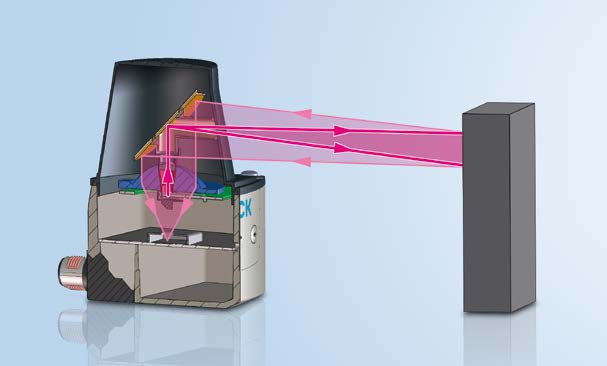
\includegraphics[width=0.55\linewidth]{Bilder/Whitepaper_LiDAR_en_IM0079963.jpg}
	\caption[Funktionsweise eines zweidimensionalen 360$^\circ$-LiDAR der Firma SICK]{Funktionsweise eines zweidimensionalen 360$^\circ$-LiDAR der Firma SICK\footnotemark}
	\label{fig:2DLaser}
\end{figure}
\footnotetext{\url{https://cdn.sick.com/media/docs/3/63/963/Whitepaper_LiDAR_en_IM0079963.PDF}, S.9}
}

\textbf{Mechanische LiDAR-Sensoren} generieren in horizontaler Ausrichtung häufig eine 360$^\circ$-Repräsentation ihrer Umgebung \cite{Weber2020}. In Abbildung \ref{fig:2DLaser} ist die Funk\-tions\-weise eines mechanischen zweidimensionalen LiDAR-Sensors dargestellt, der eine 360$^\circ$ Abbildung der Umgebung ermöglicht. Der Laserstrahl wird vertikal ausgesendet und über einen sich rotierenden Spiegel in horizontale Richtung umgelenkt. Die aus der Umgebung reflektierten Strahlen werden wieder durch den Spiegel umgelenkt und tref\-fen über eine Optik auf einen lichtempfindlichen Sensor. Über den rotierenden Spiegel wird eine schrittweise Abtastung der Umgebung erzeugt. Das Prinzip kann so er\-wei\-tert werden, dass zusätzlich eine vertikale Abtastung der Umgebung erfolgt. Dadurch wird eine dreidimensionale Vermessung erzielt. Ein Vorteil dieser Systeme ist, dass mit einem einzigen Sensor eine 360$^\circ$-Aufnahme der Umgebung erfasst werden kann. Dagegen ist ein Nachteil dieser Systeme die oft sehr große und schwere Bauweise, vor allem bei den dreidimensionalen Systemen. Außerdem wird sowohl an die Optik, als auch an die Aktorik  ein hohes Maß an Präzision gestellt. Dies macht die Systeme sehr teuer und unter Umständen wartungsaufwendig. 
 
\textbf{Solid-State Sensoren} sind in den letzten Jahren vermehrt in den Fokus der Ent\-wick\-lung gerückt \cite{FM2020}. Diese zeichnen sich im Allgemeinen durch ihre kompakte Bauweise und ihren mittlerweile vergleichsweise sehr günstigen Anschaffungspreis aus. Die halbleiterbasierte Technologie, die ohne aufwendig bewegliche Bauteile auskommt, macht sie zudem sehr robust und leicht. Nachteilig gegenüber der mechanischen Variante ist der verhältnismäßig kleine Sichtbereich. Dies kann jedoch durch die Verwendung mehrerer Sensoren in verschiedenen Ausrichtungen kompensiert werden. So können auch verschiedene Sensoren mit spezifischen Eigenschaften, wie einer hohen Reichweite in Fahrtrichtung oder einem weiten Blickwinkel im Nahbereich, dort an einem Fahrzeug kombiniert platziert werden, wo sie benötigt werden.
% Enger Blickwinkel in Ferne und breiter Blickwinkel in Nähe

\afterpage{
\begin{figure}
	\centering
	\includegraphics[width=\linewidth]{Bilder/LiDAR_Schema.png}
	\caption[Funktionsweise verschiedener Solid-State LiDAR-Sensoren]{Funktionsweise verschiedener Solid-State LiDAR-Sensoren\footnotemark}
	\label{fig:SSD_LIDAR}
\end{figure}
\footnotetext{\url{https://www.forschungsfabrik-mikroelektronik.de/de/unser-angebot/anwendungsbereiche/Transport_and_Smart_Mobility/lidar.html}}
}
 
Abbildung \ref{fig:SSD_LIDAR} zeigt die prinzipielle Funktionsweise von verschiedenen Solid-State LiDAR Technologien. Die in (a) dargestellten reinen Halbleitermodule funktionieren meist mit einem Array von Laserdioden und einem Array lichtempfindlicher Sensoren. Die Umgebung kann dabei durch eine einzige Messung erfolgen. Dies lässt eine sehr hohe Bildwiederholrate zu. Die MEMS in (b) hingegen haben bewegliche Mikrospiegel, die durch anlegen eines elektrischen Felds sehr schnell bewegt werden können. Ähnlich wie bei rein mechanischen Systemen wird die Umgebung so schrittweise abgetastet. 
  
Beide Verfahren können mit etablierten Herstellungsverfahren der Halbleiterproduktion in großen Stückzahlen vollautomatisiert hergestellt werden. Dies ermöglicht niedrige Stückpreise. Vor allem die Automobilindustrie treibt die Entwicklung der Solid-State LiDARs stark voran, da die hochauflösende Umgebungserkennung als Schlüsseltechnologie für das autonome Fahren angesehen wird. Die rein mechanischen Systeme kommen, wegen der oben aufgeführten Nachteile nicht für die Serienproduktion moderner Fahrzeuge in Frage. Auch aktuelle Top Smartphones und Tablets verfügen mittlerweile über LiDAR-Sensoren auf Basis der Solid-State Technik. Sie werden vor allem für die Verbesserung von Tiefeneffekten der Kameras, biometrische Ge\-sichts\-er\-ken\-nung und für Augmented Reality Anwendungen eingesetzt.

%
%https://www.forschungsfabrik-mikroelektronik.de/de/unser-angebot/anwendungsbereiche/Transport_and_Smart_Mobility/lidar.html
%
%https://cdn.sick.com/media/docs/3/63/963/Whitepaper_LiDAR_en_IM0079963.PDF

%\subsection{Kamera}

\subsection[RGB-D Kamera (Kopp)]{RGB-D Kamera}

RGB-D Kameras unterscheiden sich von herkömmlichen Kameras darin, dass sie zu\-sätz\-lich zum zweidimensionalen Farbbild eine Tiefeninformation registrieren können. Im Feld der mobilen Robotik hat die Technik im Gegensatz zu anderen tiefeninformationsgebenden Systemen, wie beispielsweise mechanischen LiDARs, den entscheidenden Vorteil, dass sie keine teure Kinematik mit beweglichen Bauteilen benötigen. Daher sind einige Modelle bereits für unter 200 Euro im Handel erhältlich. Auch sind viele Modelle äußerst kompakt und leicht. Zudem werden zusätzlich zur Tiefeninformation auch Farben erkannt und können ausgewertet werden. Ein Nachteil gegenüber LiDAR-Sensoren ist der eingeschränkte Blickwinkel einer einzelnen Kamera und die ver\-gleichs\-wei\-se geringe zuverlässige Reichweite von etwa 20 m. Ihre Eigenschaften machen sie zu einem beliebten Sensorsystem für mobile Roboter. Einsatzfelder sind häufig indoor-Anwedungen, bei denen Reichweiten bis zu 10 m von Interesse sind. Die Ausgabe ist je nach Kamera neben dem Farbbild eine Punktwolke oder ein Tiefenbild. Es gibt jedoch Verfahren mit denen beide Ausgaben der Tiefeninformationen ineinander überführt werden können. Außerdem kann das Farbbild mit der Punktwolke registriert werden. Dadaurch entsteht eine farbige Punktwolke.

Es gibt im Allgemeinen vier Arten wie die Tiefeinformation bei RGB-D-Kameras ermittelt werden kann. Diese sind auf Abbildung \ref{fig:RGBD_Kameras} dargestellt. 

\begin{figure}
	\centering
	\includegraphics[width=\linewidth]{Bilder/RGBD_Kameras.png}
	\caption{Darstellung der verschiedenen Techniken zur Erzeugung von Tiefeinformationen bei RGB-D Kameras}
	\label{fig:RGBD_Kameras}
\end{figure}
 
\textbf{Time of Flight Kameras} zählen zu den aktiven Sensoren, da sie die Umgebung durch aktiv ausgestrahltes Licht abtasten \cite{Shao2014}. Das Funktionsprinzip zur Gewinnung der Tiefeninformation ist gleich wie bei den Solid-State LiDARs. Abbildung \ref{fig:RGBD_Kameras} (a) zeigt den Aufbau des Systems. Es besteht aus einer Kamera und einer Lichtquelle. Die Lichtquelle sendet einen kurzen Lichtimpuls aus. Die Lichtstrahlen werden von der Umgebung reflektiert und fallen auf einen lichtempfindlichen Sensor, die Kamera, zurück. Aus der bekannten Lichtgeschwindigkeit und der Zeit, die das Licht vom Aussenden bis es auf die Kamera fällt benötigt, lässt sich so für jeden Bildpunkt eine Entfernung berechnen. Das Licht befindet sich meist im für Menschen nicht sichtbaren infraroten Bereich. Die Vorteile dieses Typs sind vor allem die hohen Bildwiederholraten von mehreren 100 Bildern pro Sekunde sowie ihr simpler Aufbau.
 
\textbf{Structured Light} wird eine Technik genannt, bei der ein Projektor ein Infrarotmuster über die Szene legt \cite{Shao2014}. Als Muster werden oft pseudo-zufällige Anordnungen von Punkten verwendet. Abbildung \ref{fig:SLBsp} zeigt ein Beispiel eines solchen Punktmusters. Durch einen Kamerasensor, der im Infrarotbereich arbeitet, wird diese Projektion wahrgenommen. Dem verarbeitenden Algorithmus ist der Abstand des Projektors zur Kamera sowie das ausgesendete Muster bekannt. Anhand des veränderten Abstands der Punkte im Bild kann durch Triangulation der Abstand dieser Punkte zur Kamera berechnet werden. Der Aufbau des Kamerasystems ist auf Abbildung \ref{fig:RGBD_Kameras} (b) dargestellt. Ein Nachteil des Systems ist die Fehleranfälligkeit durch andere Lichtquellen im gleichen Wellenbereich, wie beispielsweise das Sonnenlicht. 

\begin{figure}[htb]
	\centering
	\begin{minipage}[t]{0.45\linewidth}
		\centering
		\includegraphics[width=\linewidth]{Bilder/infrared.png}
		\caption{Beispiel eines pseudo-zufälligen Punktmusters einer Structured Light Kamera}
		\label{fig:SLBsp}
	\end{minipage}
	\hfill
	\begin {minipage}[t]{0.45\linewidth}
		\centering
		\includegraphics[width=\linewidth]{Bilder/Stereoskopie.png}
		\caption{Ermittlung der Tiefeinformation anhand der Disparität korrespondierender Bildpunkte }
		\label{fig:Stereoskopie}
	\end{minipage}
\end{figure}
 
\textbf{Passive Stereoskopie} funktioniert im Gegensatz zu den zuvor vorgestellten Verfahren ohne das Aussenden von Signalen \cite{Modrow2008}. Es handelt sich daher um ein passives Verfahren. Wie auf Abbildung \ref{fig:RGBD_Kameras} (c) zu sehen ist, werden zwei Kameras benötigt, die eine Szene aus verschiedenen Perspektiven aufnehmen. Abbildung \ref{fig:Stereoskopie} zeigt das Funktionsprinzip. Um eine Tiefeninformation zu erhalten, werden zunächst in jedem Bild Keypoints extrahiert. Diese werden verglichen, um Korrespondenzen in beiden Bildern zu finden. In der Abbildung symbolisiert das Kreuz einen Keypoint, der eine Kor\-re\-spon\-denz zwischen beiden Bildern darstellt. Anschließend wird die Disparität, die dem Unterschied der x-Koordinaten der korrespondieren Punkte entspricht, ermittelt. Da der genaue Abstand zwischen den Kameras bekannt ist, kann mit Hilfe der Dis\-pa\-ri\-tät die Entfernung jedes Keypoints zur Kamera berechnet werden.

Die passive Stereoskopie ist im Gegensatz zu den beiden vorgestellten aktiven Verfahren nicht anfällig für Fehler durch Sonnenlicht. Außerdem sind prinzipiell höhere Reichweiten realisierbar wie bei aktiven Ansätzen. Jedoch kann die Extraktion von eindeutig identifizierbaren Keypoins, beispielsweise auf einfarbigen strukturlosen Flächen, eine nicht leicht zu lösende Aufgabe darstellen, die nicht immer zu robusten Ergebnissen führt. 

\textbf{Aktive Stereoskopie} verwendet einen hybriden Ansatz, bei dem eine Kombination aus Structured Light und Stereoskopie verwendet wird \cite{Modrow2008}. Die Korrespondenzsuche wird deutlich vereinfacht, da mit Hilfe des Structured Light Ansatzes Keypoints in die Umgebung projiziert werden. Die Tiefeninformationen werden anschließend wie bei der passiven Stereoskopie ermittelt. Der Vorteil ist, dass Fehler durch  störendes Licht ausgeglichen werden können, indem auf die passive Stereoskopie zurückgegriffen wird. Außerdem können auch Entfernungen zu Oberflächen, auf denen Keypoints nur schwer oder gar nicht extrahiert werden können, bestimmt werden. 


\section[Registrierung (Kopp)]{Registrierung}

Wenn ein oder mehrere tiefeninformationsgebende Sensoren ein Objekt oder eine Umgebung aus verschiedenen Blickwinkeln aufnehmen, müssen die Punktwolken der einzelnen Messungen zusammengefügt werden. Dies wird Registrierung genannt. Da jede Punktwolke ein eigenes Koordinatensystem hat, müssen die einzelnen Punktwolken in ein gemeinsames Koordinatensystem übertragen werden. 

\subsection[Problemdefinition (Kopp)]{Problemdefinition}

Die Registrierung wird auch in der Bildverarbeitung verwendet. Beispiele für die Anwendung von Bildregistrierung sind Panoramaaufnahmen oder die dreidimensionale Rekonstruktion von Objekten. Hierbei werden mehrere Bilder einer Szene oder eines Objektes aus verschiedenen Perspektiven aufgenommen, um einen größeren Blickwinkel abzudecken oder eine dreidimensionale Abbildung eines Objektes zu erhalten. 

Ist die genaue Position des Sensors für jede Aufnahme bekannt, kann die Re\-gis\-trie\-rung auf Basis der relativen Lage der Aufnahmen zueinander durchgeführt werden. Die Positionen der Sensoren müssen dafür jedoch sehr genau gegeben sein, da bereits geringe Abweichungen dazu führen, dass die Aufnahmen nicht sinnvoll zusammengefügt werden. Eine so genaue Position der Sensoren ist nur mit hohem Aufwand zu ermitteln und in der Regel bei Anwendungen mobiler Roboter nicht gegeben. 

Es gibt verschiedene Ansätze die Registrierung auf Basis der Punktwolken durch\-zu\-füh\-ren. Um diese zusammenfügen zu können, müssen die Aufnahmen einer Szene sich in einem gewissen Bereich überlappen. Die Punktwolken werden dann so zusammengefügt, dass sie im überlappenden Bereich übereinstimmen. 

Es wird ein Koordinatensystem bestimmt, in das alle Punktwolken eingefügt werden. Häufig wird das Koordinatensystem einer der Punktwolken verwendet, die dann die Referenzpunktwolke bildet. Alle anderen Punktwolken werden an diese angefügt. Das Ergebnis der Registrierung ist die Transformation einer Punktwolke in das Re\-fe\-renz\-ko\-or\-di\-na\-ten\-sys\-tem, die die Punktwolken am besten in Übereinstimmung bringt. Diese Transformation setzt sich aus einer Rotation und einer Translation der Punktwolke zusammen. 

Abbildung \ref{fig:Registrierung} zeigt ein Beispiel zur Registrierung mehrerer Punkt\-wol\-ken. Die Punkt\-wol\-ken bilden die Struktur eines Raumes ab, der aus sechs verschiedenen Blickwinkeln aufgenommen ist. Die einzelnen Punktwolken überlappen sich teilweise. Die überlappenden Bereiche werden durch die Registrierung so übereinander gelegt, dass eine  Punktwolke entsteht, die die Umgebung abbildet. 

\afterpage{
\begin{figure}
    \centering
    \includegraphics[width=\linewidth]{Bilder/PCS_registriert.png}
    \caption[Beispiel zur Registrierung von Punktwolken]{Beispiel zur Registrierung von Punktwolken\footnotemark}
    \label{fig:Registrierung}
\end{figure}
\footnotetext{\url{https://pcl-tutorials.readthedocs.io/en/latest/registration_api.html\#registration-api}}
}

Im Kontext der mobilen Robotik wird die Registrierung von Punktwolken häufig verwendet, um die Posenschätzung eines Roboters zu erhalten oder zu verbessern. Die Posenschätzung wird auf Basis von Odometriedaten 
%oder Lokalisierungsmethoden 
getroffen, auf die in Kapitel \ref{sec:Lokalisierung} genauer eingegangen wird. Es wird dann von Scan Matching gesprochen. 

Abbildung \ref{fig:ScanMatching} zeigt eine typische SLAM-Anwendung. Eine unbekannte Umgebung wird durch einen mobilen Roboter erkundet, der ohne Informationen über seine Pose eine Karte der Umgebung erstellt. Die linke Abbildung zeigt die Karte, die nur anhand der Odometriedaten entsteht. Die rechte Abbildung zeigt die Karte, die mit Odometriedaten erstellt wird, die durch Scan Matching verbessert werden. Es ist deutlich zu sehen, dass die Schätzung der Roboterpose mit Unterstützung von Scan Matching zu besseren Resultaten führt. 
% http://kos.informatik.uni-osnabrueck.de/download/diplom/diplom.html ??

\afterpage{
\begin{figure}
    \centering
    \includegraphics[width=\linewidth]{Bilder/ScanMatching.png}
    \caption[Beispiel für die Verbesserung der Odometrie durch Scan Matching bei einer SLAM-Anwendung]{Beispiel für die Verbesserung der Odometrie durch Scan Matching bei einer SLAM-Anwendung\footnotemark}
    \label{fig:ScanMatching}
\end{figure}
\footnotetext{\url{http://ais.informatik.uni-freiburg.de/teaching/ws12/mapping/pdf/slam12-scanmatching-mini.pdf}, S.7}
}

%Die Bilder müssen sich für eine Registrierung teilweise überlappen. In diesen bereichen werden markante Punkte gesucht, dieeindeutig in beiden Bildern als Korrepsondenz identifiziert werden können. Die Bilder werden dann so aneinandergehangen, dass diese markanten Punkte aufeinander gelegt werden. 

Für die Registrierung von Punktwolken gibt es verschiedene Ansätze. Merkmal-basierte Ansätze, deren Prinzip auch in der Bildverarbeitung angewendet werden, extrahieren markante  Stellen oder Bereiche aus den Punktwolken, wie beispielsweise Punkte oder Linien \cite{Simon1994}. Anschließend werden Korrespondenzen zwischen gleichen Merkmalen in den Punktwolken gesucht. Aus den Positionen der Korrespondenzen wird die Transformation berechnet, anhand der die Punktwolken in ein gemeinsames Koordinatensystem übertragen werden können. 
% Allerdings kann es schwierig sein zuverlässig eindeutig identifizierbare Merkmale in Punktwolken zu finden. Außerdem ist die Merkmalsextraktion rechenintensiv. 

Die Registrierung kann auch als Optimierungsproblem betrachtet werden. Ein häufig verwendeter Algorithmus hierfür ist der Iterative Closest Points (ICP) Algorithmus, der im Folgenden beschrieben wird. 

\subsection[ICP (Kopp)]{ICP}

Häufig wird der ICP-Algorithmus für die Registrierung von Punktwolken verwendet. Das Ziel ist es eine Transformation zu ermitteln, die die Punktwolken mit der höchs\-ten Übereinstimmung zusammenfügt. Zu Beginn wird eine initiale Transformation geschätzt, die iterativ angepasst wird. Als Gütekriterium einer Transformation wird eine Fehlerfunktion verwendet, die minimiert wird. 
%Diese Transformation wird iterativ angenähert, indem in jedem Schritt eine neue Transformation bestimmt wird.

Es gibt viele verschiedene Variationen des ICP-Algorithmus, die sich beispielsweise in der Bestimmung der initialen Transformation oder anhand der verwendeten Fehlerfunktion unterscheiden. Ansätze für die Bestimmung der initialen Transformation sind z.B. über die Odometriedaten eines mobilen Roboters oder über eine Extraktion von korrespondierenden Merkmalen in den Punktwolken.

Alle Varianten des ICP-Algorithmus basieren jedoch auf dem gleichen Funk\-tions\-prin\-zip \cite{Rusinkiewicz2001}. 
Gegeben sind zwei Punktwolken $ P $ und $ M $, die in ein gemeinsames Koordinatensystem registriert werden sollen. Das Ziel ist eine Menge kor\-res\-pon\-die\-ren\-der Punkte in beiden Punktwolken zu finden anhand derer die gesuchte Transformation berechnet werden kann. Es wird angenommen, dass die Korrespondenz eines Punktes $ m_i \in M $ der Punkt $ p_j \in P $ ist, zu dem der euklidische Abstand minimal ist. 

\floatname{algorithm}{Algorithmus}
\begin{algorithm}
	\caption{Iterative Closest Points mit gegebenen Punktwolken $ M $ und $ P $.}
	\label{ICP}
	\begin{algorithmic}[1]
		\Function{ITERATIVECLOSESTPOINTS}{$ M,P $}
			\While{$ E  > \tau $}
				\State Berechnung der nächsten Punkte
				\State Berechnung der Transformation
				\State Anwendung der Transformation $ R,t $
				\State Berechnung des Fehlers $ E $
			\EndWhile
			\State \Return{$ R,t $}
		\EndFunction
	\end{algorithmic}
\end{algorithm}

Algorithmus \ref{ICP} zeigt den Ablauf des Grundprinzips, auf das alle Varianten des ICP-Algorithmus basieren. Zunächst wird in einer oder beiden Punktwolken eine bestimmte Menge von $ N_p $ Punkten ausgewählt, in denen die nächstgelegenen Punkte ermittelt werden. 
%Zunächst wird in einer oder beiden Punktwolken eine bestimmte Menge von $ N_p $ Punkten ausgewählt, in denen die nächstgelegenen Punkte ermittelt werden.
Basierend auf den ausgewählten korrespondierenden Punktpaaren wird die gesuchte Transformation zwischen den Punktwolken berechnet. Anschließend werden die Punktwolken anhand dieser Transformation registriert. Mit Hilfe der Fehlerfunktion wird die Güte der Transformation bestimmt.Hierfür wird beispielsweise der mittelere quadratische Fehler $ E $ aller Abstände zwischen allen Punktpaaren verwendet: 

\begin{align}
	E = \sum_i(Rp_i+t-m_i)^2
\end{align}

Dies wird solange wiederholt, bis der Fehler unter einen vorgegebenen Schwellwert $ \tau $ fällt. Dadurch wird die Transformation iterativ verbessert. 

%Werden zwei Punktwolken in ein gemeinsames Koordinatensystem registriert, werden zunächst in einer oder beiden Punktwolken eine bestimmte Menge von Punkten ausgewählt. Hierbei wird angenommen, dass die am nächsten gelegenen Punkte beider Punktwolken korrespondieren. Die Korrespondenzen werden über den euklidischen Abstand bestimmt. Es gibt verschiedene Methoden diese Korrespondenzen zu finden, beispielsweise über k-d Bäume, auf die in Kapitel ... näher eingegangen wird. Anschließend werden Paare korrespondierender Punkte in beiden Punktwolken gesucht. Bei manchen Formen des ICP-Algorithmus werden die einzelnen Punktpaare gewichtet oder einzelne Punktpaare basierend auf bestimmten Kriterien verworfen.


\section[Segmentierung (Schmelzer)]{Segmentierung}

Punktwolken setzen sich aus einer Menge von Punkten zusammen. Um aus dieser Punktmenge Informationen zu gewinnen, müssen Merkmale herausgearbeitet werden, die die vorliegende Punktwolke beschreiben. Hierfür gibt es verschiedene Ansätze.
%, über die in Kapitel \ref{Merkmale} ein Überblick gegeben wird. 
Die Basis einiger Verfahren zur Merkmalsextraktion aus Punktwolken bildet die Segmentierung. Hierbei werden aus den Punkten Gruppen zusammengehöriger Informationen herausgearbeitet. Die Segmentierung wird beispielsweise bei der Objekterkennung verwendet, um die Punkte zusammenzufassen, die gemeinsam  ein Objekt bilden. 

Durch die Zerlegung einer großen in mehrere kleinere Punktwolken, sogenannte Segmente, ergeben sich einige Vorteile in der Weiterverarbeitung. So lassen sich Algorithmen effizienter anwenden, da die Verarbeitung von kleineren Punktwolken schneller ist. Außerdem können die Segmente auch parallel weiterverarbeitet werden. Die Punkt\-wol\-ke kann auch gefiltert werden, sodass in der Weiterverarbeitung nur relevante Segmente verwendet werden. Wenn beispielsweise verschiedenen Objekte auf einem Tisch erkannt werden sollen, könnte die Punktwolke so gefiltert werden, dass das Segment der Tischoberfläche weg fällt. Zusätzlich wird weniger Speicherplatz benötigt, wenn z.B. Rauschen reduziert wird durch das Löschen von Punkten, die keinem Segment zugewiesen wurden. 

Die Segmentierung wird nicht nur zur Verarbeitung von Punktwolken eingesetzt, sondern ist auch ein Teilgebiet der  Bildverarbeitung. Hier wird sie ebenfalls als Vorstufe der Merkmalsextraktion verwendet. Bei der Segmentierung von Bildern werden teilweise ähnliche Verfahren verwendet wie bei der Segmentierung von Punktwolken. 

\subsection[Segmentierung in der Bildverarbeitung (Schmelzer)]{Segmentierung in der Bildverarbeitung}
%https://link.springer.com/content/pdf/10.1007%2F978-3-642-04952-1.pdf

In der Bildverarbeitung werden Bilder bei der Segmentierung in Regionen unterteilt, indem die Pixel anhand vorgegebener Kriterien verschiedenen Gruppen zugeordnet werden. Die Anzahl der sich so ergebenden Regionen ist nicht fest vorgegeben, sondern abhängig vom zugrundeliegenden Bild und des verwendeten Verfahrens. Sie wird beispielsweise als Vorstufe der Objekterkennung eingesetzt, um Objekte vom Hintergrund zu separieren. 

Für die Segmentierung gibt es verschiedene Ansätze bei denen im wesentlichen Pixel-, Kanten- und Regionen-basierte Verfahren unterschieden werden.
%Die Aufteilung eines Bildes in verschiedene Regionen kann auf Basis eines Schwellwerts für die Pixelwerte vorgenommen werden oder durch das Erkennen von Kanten. Eine weitere Methoden bildet das Region Growing  , die die Kriterien definieren anhand derer das Bild unterteilt wird.  

\subsubsection[Pixel-basierte Segmentierung (Schmelzer)]{Pixel-basierte Segmentierung}

Bei der Pixel-basierten Segmentierung werden Bildregionen anhand der  einzelnen Pi\-xel\-wer\-te, die den Helligkeitswerten bei Graustufenbildern entsprechen, unterschieden \cite{Jaehne2012}. Es wird jeder einzelne Pixel geprüft, ob sein Wert einen vorgegeben Grenzwert übersteigt und  entsprechend einer Gruppe zugewiesen. Es werden also die hellen und dunklen Bildbereiche unterschiedenen. Dadurch bilden sich zwei Bild\-be\-rei\-che heraus. Die Güte des Verfahren ist abhängig von der Wahl des  Grenzwerts, der anhand des Histogramms der Grauwerte eines Bildes gewählt wird. 

Abbildung \ref{fig:seg2d} zeigt ein Beispiel anhand des Bildes aus Abbildung \ref{fig:pc}. In (a) ist das Ausgangsbild zu sehen, das in ein Graustufenbild umgewandelt wurde. Anschließend wird es anhand der Intensitätswerte in zwei Bildbereiche unterteilt. In (b) ist das zugehörige segmentierte Bild dargestellt. Das Bild zeigt, dass das Verfahren abhängig von der Homogenität der Bildbereiche ist. Bei nicht homogenen Hintergründen und Objekten mit verschiedenen Helligkeitswerten verschmelzen durch die verschiedenen Helligkeitsstufen die Grenzen zwischen diesen und es kommt zu Löchern in den Bildregionen. Eine eindeutige Trennung eines Objektes vom Hintergrund ist dadurch nur in bestimmten Fällen möglich, beispielsweise bei der Herausarbeitung von Buchstaben oder Ziffern. 

Es handelt sich um ein simples Verfahren, das nur wenig Rechenleistung benötigt. Allerdings sind die Anwendungsbreiche eingeschränkt, da nur gute Ergebnisse erzielt werden können, wenn die verschiedenen Bildbereiche möglichst homogen sind. Außerdem ist das Verfahren abhängig von der Beleuchtung, da diese auch in homogenen Bildbereichen zu einer Abstufung der Grauwerte führen kann. Die An\-wen\-dungs\-be\-rei\-che beschränken sich daher auf Bilder, in denen die zu trennenden Bereiche deutliche Unterschiede aufweisen und homogen sind. Zudem kann die Größe eines Objekts nicht genau bestimmt werden, da diese durch leichte Grauwertabstufungen  in Randbereichen abhängig vom gewählten Grenzwert variiert. 

\begin{figure}
    \centering
    \includegraphics[width=\linewidth]{Bilder/Segmentierung2D.png}
    \caption{Beispiele zur Segmentierung in der Bildverarbeitung anhand des Bildes in (a) basierend auf (b) einen Schwellwert und (c) durch Kantenerkennung}
    \label{fig:seg2d}
\end{figure}

\subsubsection[Kanten-basierte Segmentierung (Schmelzer)]{Kanten-basierte Segmentierung}

Kanten-basierte Segmentierungsverfahren grenzen Bildbereiche durch das Erkennen von Kanten voneinander ab  \cite{Jaehne2012}. Diese zeichnen sich in Bildern durch Diskontinuitäten in den Helligkeitswerten aus. Die Positionen von Kanten werden mit Hilfe des Grauwertgradienten ermittelt. Kanten zeigen sich in der Ableitung erster Ordnung durch Extremwerte.
% und in der Ableitung zweiter Ordnung durch einen Nulldurchgang. Daher werden Kanten durch 
Daher wird bei der Kanten-basierten Segmentierung nach lokalen Maxima im Betrag des Grauwertgradienten gesucht. Häufig werden auch Kantenverfolgungsalgorithmen eingesetzt, die die Kanten entlang eines Objekts verfolgen sobald ein lokales Maximum gefunden wird. Die sich so ergebenden verschiedenen Bild\-be\-rei\-che werden durch die Kanten voneinander getrennt. Abbildung \ref{fig:seg2d} (c) zeigt ein Beispiel zur Kantenerkennung anhand des in (a) abgebildeten Graustufenbildes. 

Die Kanten-basierte Segmentierung eignet sich im Vergleich zur Pixel-basierten Segmentierung besser für Anwendungen bei denen die Größe der segmentierten Be\-rei\-che von Bedeutung ist, da diese anhand der Kante besser bestimmt werden kann. Die Segmentierung liefert bessere Ergebnisse, je höher der Kontrast eines Objektes zum Hintergrund ist. Verschmierte Kanten mit weniger Kontrast liefern hingegen schlechtere Ergebnisse, da der Gradient in diesen Bereichen kleiner ausfällt. 

\subsubsection[Regionen-basierte Segmentierung (Schmelzer)]{Regionen-basierte Segmentierung}

Für die Regionen-basierte Segmentierung gibt es verschiedene Verfahren, wie bei\-spiels\-wei\-se das Region Growing \cite{Burger2015}. Hierbei wachsen Bildregionen schritt\-wei\-se ausgehend von einem initialen Pixel. Benachbarte Pixel werden auf Basis eines vorgegeben Homogenitätskriterium zusammengefasst. Ein Kriterium kann bei\-spiels\-wei\-se ein Grenz\-wert auf die Differenz der Grauwerte sein. Wenn das Kriterium zu einem benachbarten Pixel erfüllt ist, wird dieser Pixel zu der Region hinzugefügt. Dies wird rekursiv wiederholt indem von den hinzugefügten Pixeln auf gleiche Weise wei\-ter gewachsen wird. Eine Region ist abgeschlossen, wenn keine weiteren Pixel mehr hinzukommen, da die benachbarten Punkte das Kriterium nicht erfüllen. Anschließend kann dies für weitere initiale Pixel wiederholt werden bis alle Pixel eines Bildes einer Region zugefügt sind. 
%http://users.cs.cf.ac.uk/Dave.Marshall/Vision_lecture/node35.html
%https://link.springer.com/content/pdf/10.1007%2F978-3-642-04952-1.pdf S. 547
%https://link.springer.com/content/pdf/10.1007%2F978-3-642-04604-9.pdf .  224

Für die  Wahl der initialen Pixel gibt es verschiedene Ansätze, die zum Herausbilden unterschiedlicher Regionen führen können. Um die Segmentierung zu beschleunigen, können die Pixel vor dem Region Growing in ein regelmäßiges Gitter mit fester Kantenlänge eingefügt werden. Dadurch ergeben sich Zellen gleicher Größe, beispielsweise von 4$\times$4  Pixeln. Die Segmente wachsen dann nicht von Pixel zu Pixel, sondern von einer Gitterzelle zur anderen. Dadurch werden weniger Rekursionen benötigt, um das ganze Bild in Regionen aufzuteilen. Abhängig vom gewählten Kriterium kann es al\-ler\-dings vorkommen, dass Regionen zusammenwachsen, die eigentlich getrennt sind. Dies passiert, wenn diese nur in kleinen Bereichen, beispielsweise nur zwischen zwei Pixeln das Kriterium erfüllen. Bei Gitter-basiertem Region Growing wird dies zusätzlich von der gewählten Kantenlänge beeinflusst. 

\subsection[Segmentierung von Punktwolken (Schmelzer)]{Segmentierung von Punktwolken}

Bei der Segmentierung von Punktwolken werden diese häufig in eine Gitterstruktur mit gleichmäßigen Kantenlängen eingefügt. Die einzelnen Zellen eines Gitters werden im zweidimensionalen Raum als Pixel bezeichnet, im dreidimensionalen als Voxel. Dadurch kann die Anzahl der Punkte reduziert werden, indem die Punkte in einem Pi\-xel bzw. Voxel zusammengefasst werden. Die Segmentierungsalgorithmen können in diesen Fällen auf die einzelnen belegten Pixel bzw. Voxel angewendet werden. Außerdem werden Punktwolken dadurch in eine regelmäßige Struktur gezwungen, wie sie auch bei Bildern durch die Einteilung in Pixel gegeben ist. Zusätzlich kann Speicherkapazität gespart werden, indem die Punktwolken in effizienten Datenstrukturen ge\-spei\-chert werden, wie beispielsweise Octrees, die belegte und freie Bereiche in Voxelgittern effizient zusammenfassen.

Das Prinzip einiger Segmentierungsmethoden aus der Bildverarbeitung kann auch auf Punktwolken übertragen werden. So gibt es z.B. auch Kanten-basierte Segmentierungsverfahren. Kanten zeichnen sich in Punktwolken z.B. durch starke Richtungsänderungen der Normalenvektoren oder große Differenzen in den Schätzungen der Krümmungswerte eines Punktes aus \cite{Wilke2002}. Die Krümmung eines Punktes wird hierbei durch die Krümmung der Fläche seiner Nachbarschaft geschätzt. Auch der Normalenvektor eines Punktes wird über diese Nachbarschaft ermittelt. 

Auch das Prinzip des Region Growing kann auf Punktwolken angewendet werden. Wie in der Bildverarbeitung basiert es auf dem Zusammenwachsen benachbarter Punkte, wenn diese bestimmte Kriterien erfüllen. Eine Region ist abgeschlossen sobald keine weiteren Punkte mehr hinzukommen, da sie die Bedingungen nicht erfüllen. Region Growing Algorithmen arbeiten auf Basis der Nachbarschaft eines Punktes. Daher werden die Punktwolken häufig vor der Segmentierung in effizienten Datenstrukturen, wie $k$-d-Bäumen, gespeichert, da diese die Ermittlung der benachbarten Punkte beschleunigen. Auf $k$-d Bäume und die Suche der benachbarten Punkte in diesen wird in Kapitel \ref{sec:k-d-baum} näher eingegangen. 
% Segmentierung anhand mehrerer Punkte statt nur durch Randpunkte wie bei kanten-basierten Segmenteirungsverfahren. Zuordnung der Randpunkte kann unsicher sein bei nahe gelegenen Segmenten. Jeder innere Punkt gehört jedoch nur zu einem Segment. Dadurch ist Mehrzahal der Punkte eindeutig zurordbar

Es gibt verschiedene weitere Ansätze zur Segmentierung von Punktwolken. Im folgenden werden zwei gängige Verfahren auf Basis des Region Growings erläutert, die auch in der PCL implementiert sind. Die Zuordnung der Punkte in verschiedene Regionen wird auch als Clustering bezeichnet und die entstehenden Regionen dem\-ent\-spre\-chend als Cluster. 

%Um die Nachbarschaft jedes Punktes effizient ermitteln zu können, werden die Punktwolken häufig in eine Gitterstruktur eingefasst und anschließend in eine effiziente Datenstruktur, wie bes 

\subsubsection[Euklidisches Clustern (Schmelzer)]{Euklidisches Clustern}

Beim Region Growing durch euklidisches Clustern werden benachbarte Punkte zu ei\-ner Region zusammengefasst, deren euklidische Abstände unterhalb eines vorgegebenen maximalen Abstands liegen. 

%http://www.pointclouds.org/documentation/tutorials/cluster_extraction.php#cluster-extraction
Algorithmus \ref{euklid} zeigt den Pseudocode des in der PCL verwendeten euklidischen Clustering von Punktwolken \cite{Rusu2009}. In Zeile 2 werden leere Mengen für die Cluster $ C $ und die Punkte $ Q $, die geprüft werden müssen, ob von ihnen aus weiter gewachsen wird, erstellt. Ab Zeile 3 werden in einer Schleife alle Punkte der Punktwolke $ P $ durchlaufen und die Cluster beginnen zu wachsen. Ab Zeile 7 wird für jeden Punkt die Nachbarschaft $ P_i^k $ ermittelt. Zu dieser gehören alle Punkte, die innerhalb eines Radius $ d_{th} $ vom aktuellen Punkt $ p_i $ aus liegen. Anschließend wird jeder Punkt der Nachbarschaft, der noch nicht in $ Q $ enthalten ist, in diese Menge hinzugefügt. Für alle Punkte in $ Q $ wird ab Zeile 5 in einer Schleife geprüft, ob das aktuelle Cluster von diesen Punkten aus weiter wächst. Die Menge $ Q $ enthält also alle Punkte, die zu einem Cluster gehören. Wenn das aktuelle Cluster nicht mehr weiter wächst, wird die Menge $ Q $ als Cluster in die Menge aller Cluster $ C $ geschrieben. Die Menge $ Q $ wird dann wieder geleert und ein neues Cluster beginnt von einem anderen Punkt aus $ P $  zu wachsen. Dies wird solange wiederholt bis alle Punkte der Punktwolke durchlaufen sind und somit jeder Punkt einem Cluster zugewiesen ist. 
%Die Suche der benachbarten Punkte kann mit unterschiedlichen Methoden erfolgen. Eine effiziente Methoden hierfür ist es, wenn vor dem Clustern beispielsweise eine kd-Baum Repräsentation der Punktwolke $ P $ erstellt wird. Hierauf wird in Kapitel 
%In der PCL werden die Punkte vor dem eigentlichen Clustern zunächst in eine Gitterstruktur eingefügt und 
%
%http://mediatum.ub.tum.de/doc/800632/941254.pdf S.98ff
\floatname{algorithm}{Algorithmus}
\begin{algorithm}
	\caption{Euklidisches Clustering mit gegebener Punktwolke $ P $ und Radius $ d_{th} $.}
	\label{euklid}
	\begin{algorithmic}[1]
		\Function{EUCLIDEANCLUSTERING}{$ P,d_{th} $}
			%\State Erstelle eine Kd-Baum Repräsentation von $ P $
			\State $ C \leftarrow \emptyset, Q \leftarrow \emptyset $
			\ForEach{$ p_i \in P $}
				\State $ Q \leftarrow p_i $
				\ForEach{$ p_i \in Q $}
					\State $ P_i^k \leftarrow \emptyset $
					\ForEach{$ p_j \in P $}
						\If{$ min \Vert p_i-p_j \Vert \leq d_{th} $}
							\State $ P_i^k \leftarrow p_j $
						\EndIf
					\EndFor
					\ForEach{$ p_i^k \in P_i^k $}
						\If{$ p_i^k \notin Q $}
							\State $ Q \leftarrow p_i^k $
						\EndIf
					\EndFor
				\EndFor
				\State $ C \leftarrow Q $
				\State $ Q \leftarrow \emptyset $
			\EndFor
			\State \Return{$ C $}
		\EndFunction
	\end{algorithmic}
\end{algorithm}

%\floatname{algorithm}{Algorithmus}
%\begin{algorithm}
%	\caption{Euklidisches Clustering mit gegebener Punktwolke $ P $ und Radius $ d_{th} $.}
%	\label{SC}
%	\begin{algorithmic}[1]
%		\Function{EUCLIDEANCLUSTERING}{$ P,d_{th} $}
%			\State $ R \leftarrow \emptyset, \{A\} \leftarrow \{1,...,\vert P \vert \} $
%%			\While{$ \{A\} \neq \emptyset $}
%			\ForEach{$ p_i \in \{A\} $}
%				\State $ \{R_c\} \leftarrow \emptyset $
%				\State $ \{R_c\} \leftarrow \{R_c\} \cup p_i $
%				\State $ \{A\} \leftarrow \{A\} \setminus p_i $
%				\For{$ j=0 $ to $ size(\{R_c\}) $}
%					\State $ \{B_c\} \leftarrow \Omega(R_c{j}) $
%					\For{$ k=0 $ to $ size(\{B_c\}) $}
%						\State $ p_k \leftarrow B_c\{k\} $
%						\If{$ p_k \in \{A\} $ \& $ min \Vert p_i-p_k \Vert \leq d_{th} $}
%							\State $ \{R_c\} \leftarrow \{R_c\} \cup p_k $
%							\State $ \{A\} \leftarrow \{A\} \setminus p_k $
%						\EndIf
%					\EndFor
%				\EndFor
%				\State $ \{R\} \leftarrow \{R\} \cup \{R_c\} $
%			\EndFor
%%			\EndWhile
%			\State \Return{$ \{R\} $}
%		\EndFunction
%	\end{algorithmic}
%\end{algorithm}

\subsubsection[Flächen-basiertes Clustern (Schmelzer)]{Flächen-basiertes Clustern}

Beim Region Growing durch Flächen-basiertes Clustern werden Segmente durch Punkte gebildet, die eine Fläche aufspannen und dadurch ähnliche geometrische Eigenschaften aufweisen. Als Bedingung für das Zusammenwachsen werden beispielsweise ähnliche Krümmungswerte oder Normalenvektoren der Punkte verwendet. Diese werden üblicherweise für jeden Punkt über die Fläche, die durch die Punkte seiner Nachbarschaft entsteht, geschätzt. 

Für die Auswahl der initialen Punkte, von denen aus Segmente beginnen zu wachsen, gibt es verschiedene Vorgehensweisen. Beispielsweise wird für die Krümmung der Punkte ein Grenzwert festgelegt und nur Punkte, deren Krümmungswert unterhalb dieser Grenze liegt, werden als Startpunkt für das Region Growing verwendet. Die Auswahl kann jedoch auch zufällig sein. 

Die entstehenden Segmente können nicht nur ebene Flächen darstellen, sondern  auch gekrümmte Flächen, wie z.B. die Mantelfläche eines Zylinders. Allerdings können auch beliebige polynomiale Flächen approximiert werden \cite{Wilke2002}. Hierfür wird über alle Punkte einer Region eine Approximationsfläche berechnet. Benachbarte Punkte werden nur hinzugefügt, wenn der mittlere Approximationsfehler an eine vorgegebene Referenzfläche einen bestimmten Grenzwert nicht übersteigt. Nachteilig bei dieser Vorgehensweise ist jedoch, dass eine Referenzfläche gegeben sein muss, aus der die geometrischen Beziehungen zwischen den Punkten abgeleitet werden. Dadurch ist das Verfahren nicht allgemein anwendbar, sondern setzt ein Wissen über das gewünschte Segment voraus. Außerdem ist dieser Ansatz vergleichsweise rechenintensiv, da nach jedem Hinzufügen eines Punktes eine neue Approximationsfläche berechnet werden muss.
% Approximation von Flächen

In der PCL wird als Kriterium für das Region Growing ein Grenzwert auf den Winkel zwischen den Normalenvektoren zweier Punkte verwendet \cite{PCLRG2020}. Es werden Segmente gebildet, die flache Ebenen repräsentieren. Hierbei werden zunächst alle Punkte nach ihren Krümmungswerten sortiert, da das Region Growing bei dem Punkt mit dem niedrigsten Krümmungswert beginnt. Dadurch wachsen Segmente immer vom flachsten Punkt aus. Zusätzlich ist ein Grenzwert auf den Krümmungswert der Punkte festgelegt und Segmente wachsen nur von Punkten mit einem geringeren Krümmungswert. Somit wird die Anzahl der Segmente insgesamt verringert als beispielsweise bei einer zufälligen Wahl der initialen Punkte. 
%http://www.pointclouds.org/documentation/tutorials/region_growing_segmentation.php#region-growing-segmentation

\floatname{algorithm}{Algorithmus}
\begin{algorithm}
	\caption{PCL Region Growing auf Basis der Smoothness Constraints mit gegebener Liste der sortierten Punkte der Punktwolke $ \{P\} $, der Normalen $ \{N\} $ und Krümmungen $ \{c\} $ aller Punkte, der Funktion zur Ermittlung der Nachbarschaft $ \Omega $ und den Grenzwerten für die Krümmung $ c_{th} $ sowie den Winkel $ \theta_{th} $ der Normalen.}
	\label{SC}
	\begin{algorithmic}[1]
		\Function{SMOOTHNESSCONSTRAINTS}{$ \{P\},\{N\},\{c\},\Omega,c_{th},\theta_{th} $}
			\State $ R \leftarrow \emptyset, \{A\} \leftarrow \{1,...,\vert P \vert \} $
			\While{$ \{A\} \neq \emptyset $}
				\State $ \{R_c\} \leftarrow \emptyset $
				\State $ \{S_c\} \leftarrow \emptyset $
				\State $ \{A\} \rightarrow P_{min} $
				\State $ \{S_c\} \leftarrow \{S_c\} \cup P_{min} $
				\State $ \{R_c\} \leftarrow \{R_c\} \cup P_{min} $
				\State $ \{A\} \leftarrow \{A\} \setminus P_{min} $
				\For{$ i=0 $ to $ size(\{S_c\}) $}
					\State $ \{B_c\} \leftarrow \Omega(S_c{i}) $
					\For{$ j=0 $ to $ size(\{B_c\}) $}
						\State $ P_j \leftarrow B_c\{j\} $
						\If{$ P_j \in \{A\} $ \& $ cos^{-1}(\vert (N\{S_c\{i\}\},N\{S_c\{ j\}\}) \vert) < \theta_{th} $}
							\State $ \{R_c\} \leftarrow \{R_c\} \cup P_j $
							\State $ \{A\} \leftarrow \{A\} \setminus P_j $
							\If{$ c\{P_j\} < c_{th} $}
								\State $ \{S_c\} \leftarrow \{S_c\} \cup P_j $
							\EndIf
						\EndIf
					\EndFor
				\EndFor
				\State $ \{R\} \leftarrow \{R\} \cup \{R_c\} $
			\EndWhile
			\State \Return{$ \{R\} $}
		\EndFunction
	\end{algorithmic}
\end{algorithm}

Algorithmus \ref{SC} zeigt den Pseudocode des auf ebenen Flächen basierenden Region Growing Verfahrens der PCL. Dieser wird angewendet nachdem die Punkte der Punkt\-wol\-ke bereits nach aufsteigenden Krümmungswerten sortiert und in einer Liste $ \{P\} $ gespeichert sind. Außerdem sind bereits die Krümmung $ \{c\} $ und die Normale $ \{N\} $ jedes Punktes berechnet. In Zeile 2 wird eine leere Menge der Regionen $ R $ erstellt sowie die Indizes aller Punkte in einer Liste der verfügbaren Punkte $ \{A\} $ gespeichert. Diese enthält alle Punkte, die noch keiner Region zugewiesen wurden. Anschließend wachsen in einer Schleife die Segmente. 

Zunächst werden in Zeile 4 und 5 leere Listen der aktuellen Region $ \{R_c\} $ sowie der aktuellen Samen $ \{S_c\} $ angelegt. In Zeile 6 bis 9  wird aus der Liste der verfügbaren Punkte der Punkt mit dem minimalsten Krümmungswert gezogen und der Liste der aktuellen Samen $ \{S_c\} $ und Region $ \{R_c\} $ hinzugefügt. Aus der Liste der verfügbaren Punkte $ \{A\} $ wird dieser entfernt. 

Anschließend werden ab Zeile 10 in einer Schleife für alle aktuellen Samen $ \{S_c\} $ die jeweilige Nachbarschaft $ \{B_c\} $ in der Punktwolke $ P $ über die Funktion $ \Omega $ ermittelt. In einer weiteren Schleife wird ab Zeile 12 für jeden Punkt der Nachbarschaft geprüft, ob dieser bereits einer Region zugewiesen wurde und der Winkel zwischen seiner Normalen und der des aktuellen Samens $ \{S_c\} $ unterhalb des vorgegebenen Grenzwerts $ \theta_{th} $ liegt. Wenn dies der Fall ist, wird der Punkt in Zeile 15 der aktuellen Region $ \{R_c\} $ hinzugefügt und in Zeile 16 aus der Liste der verfügbaren Punkte $ \{A\} $ entfernt. Anschließend wird der Punkt in Zeile 18 zur Liste der aktuellen Samen $ \{S_c\} $ hinzugefügt, wenn sein Krümmungswert $ c $ kleiner als der Schwellwert $ c_{th} $ ist. 

Eine Region ist abgeschlossen, wenn keine Punkte mehr hinzukommen. Dies ist der Fall wenn alle Samen der Region durchlaufen sind und kein weiterer Punkt die Bedingung erfüllt, ein Samen zu werden. Die aktuelle Region $ \{R_c\} $ wird dann in Zeile  19 der Menge der Regionen $ \{R\} $ hinzugefügt. Das Verfahren beginnt erneut mit der Auswahl des Punktes mit minimalem Krümmungswert aus der Liste der verfügbaren Punkte $ \{A\} $. Der Algorithmus endet, wenn alle Punkte einer Region zugeordnet wurden und daher die Liste der verfügbaren Punkte $ \{A\} $ leer ist. 

%Anschließend werden ab Zeile 10 in einer Schleife für alle aktuellen Samen $ \{S_c\} $ die jeweilige Nachbarschaft über die Funktion $ \Omega $ ermittelt und in einer Liste $ \{B_c\} $ gespeichert. In einer weiteren Schleife wird für jeden Punkt der Nachbarschaft geprüft, ob der Winkel zwischen seiner Normalen und der des aktuellen Samens unterhalb des vorgegebenen Grenzwerts $ \theta_{th} $ liegt. Wenn dies der Fall ist wird der Punkt der aktuellen Region hinzugefügt und aus der Liste der verfügbaren Punkte entfernt. Anschließend wird der Punkt zur Liste der aktuellen Samen hinzugefügt, wenn sein Krümmungswert kleiner als der Schwellwert $ c_{th} $ ist. Eine Region ist abgeschlossen, wenn keine Punkte mehr hinzukommen. DIes ist der Fall wenn alle Samen der Region durchlaufen sind unf kein weiterer Punkt die Bedingung erfüllt, ein Samen zu werden. Die Region wird dann der Menge der Regionen hinzugefügt und das Verfahren beginnt erneut mit dem Punkt der Liste der verfügbaren Punkte, dessen krümmungswert minimal ist. Der Algorithmus endet, wenn alle Punkte einer   Region zugeordnet wurden und daher die Liste der verfügbaren Punkte leer ist. 

%\section{Merkmalsextraktion/ Beschreibung von Punktwolken}
%\label{Merkmale}

\section[$k$-d-Bäume (Schmelzer)]{$k$-d-Bäume}
\label{sec:k-d-baum}

Häufig ist es nötig in Punktwolken nach Punkten zu suchen die ein bestimmtes Kriterium erfüllen. Dies kann beispielsweise die Suche nach dem nächstgelegenen Nachbarn eines Punktes sein. Dies ist der Punkt, der den geringsten Abstand zu diesem hat. Dies wird z.B. bei ICP benötigt. Ebenso können auch alle Punkte gesucht sein, die innerhalb eines vorgegebenen Bereichs liegen, wie z.B. bei der Suche aller Nachbarpunkte eines Punktes, die innerhalb eines vorgegebenen Radius liegen. Wie bereits erwähnt, wird dies sowohl bei der Flächen-basierten Segmentierung als auch beim euklidischen Clustering benötigt. 

Punktwolken setzen sich häufig aus einer großen Menge an Punkten zusammen. Die Suche nach Punkten ist sehr ineffizient, wenn alle Punkte der Punktwolke auf die Erfüllung des vorgegebenen Kriteriums untersucht werden müssen. Daher werden diese in effizienten Datenstrukturen abgespeichert, die eine wesentlich schnellere Suche ermöglichen.

$k$-d-Bäume stellen eine solche effiziente Datenstruktur zur organisierten Speicherung von $k$-dimensionalen Punktwolken dar. Dies ist ein $k$-dimensionaler binärer Suchbaum. Das Ziel ist es bei der Suche nach bestimmten Punkten in einem $k$-d-Baum ganze Teilbäume wegfallen zu lassen, deren Punkte das vorgegebene Kriterium nicht erfüllen. Somit wird die Menge der Punkte, deren Lage bei der Suche geprüft werden müssen, wesentlich reduziert im Vergleich zur  Suche in der gesamten Punktwolke. 
%Mit Hilfe einer binären Suche kann in einem k-d-Baum effizient nach bestimmten Punkten gesucht werden

Da Punktwolken auch die Einträge von Datenbanken oder Merkmalsvektoren, die eine Punktwolke beschreiben, darstellen können, werden $k$-d-Bäume auch in diesen Bereichen häufig angewendet. 

\subsection[Aufbau (Schmelzer)]{Aufbau}

Ein $k$-d-Baum weist die aus der Graphentheorie bekannte Struktur eines Baums auf. Da jeder Knoten maximal zwei Kindknoten haben kann, ist dieser binär. In jedem Blatt wird ein Punkt $ p_i$ der $k$-dimensionalen Punktwolke $ \mathcal{P} $ gespeichert. Die Wurzel sowie die inneren Knoten stellen Entscheidungspunkte dar. Der Wert eines Entscheidungsknoten wird als Splitwert $ s $ bezeichnet, der einer bestimmten Koordinatenachse, wie z.B. der $x$-Koordinate, zugeordnet ist \cite{Klein2005}. Durch einen Vergleich des entsprechenden Koordinatenwerts jedes Punkts $ p_i $ mit dem Splitwert $ s $ wird entschieden, ob $ p_i $ links oder rechts von diesem Knoten gespeichert wird.
%anhand dessen entschieden wird, ob ein Punkt $ p_i $ links oder rechts von diesem Knoten gespeichert wird. 
%, anhand deren Wert $ s $ entschieden wird, ob ein Punkt $ p_i $ links oder rechts von diesem Knoten gespeichert wird. 

An jedem Entscheidungsknoten wird die Punktwolke in zwei möglichst gleich große Teilpunktmengen $ D_{<s} $ und $ D_{>s} $ geteilt \cite{Klein2005}. Alle Punkte deren Wert der Koordinate von $ s $ größer als $ s $ ist, werden der Menge $ D_{>s} $ und alle übrigen  Punkte der Menge $ D_{<s} $ zugewiesen. Dies wird mit Hilfe einer $ (k-1) $-dimensionalen Hyperebene realisiert, die am Splitwert $ s $ orthogonal zur Koordinatenachse von $ s $ ist. Die Hyperebene trennt den Merkmalsraum. Am Beispiel einer zweidimensionalen Punktwolke mit einem Splitwert $ s $ bezüglich der $x$-Koordinaten ergeben sich folgende Teilmengen: 

\begin{align}
\begin{split}
	D_{<s} = \{(x,y) \in D;x<s\} \\
	D_{>s} = \{(x,y) \in D;x>s\}
\end{split}
\end{align} 

In der nächsten Ebene des Baums werden die Teilpunktmengen anhand einer anderen Splitkoordinaten separiert. Wenn alle Koordinaten durchlaufen sind, wird wieder bei der ersten Korrdinate begonnen. Dies wird solange wiederholt, bis jede Teilpunktwolke nur noch einen Punkt enthält. 

Abbildung \ref{fig:k-d-Baum} zeigt den Aufbau eines $k$-d-Baums am Beispiel einer zweidimensionalen Punktwolke. Im $ \mathbb{R}^2 $ wird der Merkmalsraum durch eine Gerade getrennt. In (a) ist die Punktwolke  samt Trenngeraden in ein $x,y$-Koordinatensystem eingezeichnet. In (b) ist der zugehörige $2$-d-Baum abgebildet. 

\begin{figure}
    \centering
    \includegraphics[width=\linewidth]{Bilder/kd_Baum.png}
    \caption{Aufbau eines $k$-d-Baums am Beispiel einer zweidimensionalen Punktwolke}
    \label{fig:k-d-Baum}
\end{figure}

Die erste Trenngerade steht senkrecht auf der $x$-Achse und separiert die Punktwolke an der Stelle $ x=5 $. Dies ist der Splitwert $ s $ der ersten Ebene des Baums und wird daher als Wurzel in den Baum eingetragen. Der Splitwert wird so gewählt, dass die entstehenden Teilmengen etwa die gleiche Anzahl an Punkten umfassen. Die sich ergebende Teilmenge $ D_{<5} $ befindet sich auf der linken Seite der Trennebene und daher auch im linken Teilbaum nach der Wurzel, die Teilmenge $ D_{>5} $ wird im rechten Teilbaum gespeichert. 

Anschließend werden in der nächsten Ebene des Baums beide Teilmengen or\-tho\-go\-nal zur $y$-Achse geteilt. Für $ D_{<5} $ ergibt sich eine Trennebene bei $ y=6,5$ und für $ D_{>5} $ bei $y=5$. Die sich ergebenden Teilmengen werden in der nächsten Ebenen abwechselnd erneut orthogonal zur $x$-Achse und anschließend orthogonal zur $y$-Achse getrennt. Dies wiederholt sich bis jeder Punkt jeweils in einem Blatt gespeichert wird. 
% Trennung so dass möglichst zwei gleich große Punktwolken entstehen -> mittelwert über Punktmenge

Ein $k$-d-Baum, dessen Hyperebenen die Punktmengen immer in etwa gleich große Teilmengen trennt, wird als ausgeglichen bezeichnet. Der Baum und alle Teilbäume aus denen er sich zusammensetzt, weisen auf beiden Seiten der Wurzel etwa \linebreak gleich viele Blätter auf. Um einen ausgeglichenen $k$-d-Baum aufzubauen, wird jeder Splitwert $ s $ durch den Median aller Punkte in Richtung der Splitkoordinaten gebildet \cite{Berg2008}. Dieser entspricht dem $ \dfrac{n}{2} $-st kleinsten Wert aller $ n $ Punkte der Punktmenge. Um diesen effizient ermitteln zu können, werden die Punkte häufig vorher in Richtung jeder Koordinaten sortiert. Es ergeben sich dann $k$ sortierte Listen der Punktwolke $ \mathcal{P} $.  

Ein ausgeglichener $k$-d-Baum stellt die effizienteste Anordnung eines $k$-d-Baums verglichen mit unausgeglichenen Varianten der gleichen Punktwolke dar. Er benötigt zur Speicherung von $n$ Punkten einer $k$-dimensionalen Punktwolke einen Speicher von $ O(n) $. Die Hohe des Baumes ist durch $ O(log n) $ beschränkt. Daraus ergibt sich, dass ein ausgeglichener $k$-d-Baum in einer Zeit von $ O(n log n) $ konstruiert werden kann. 

%Baum erstellen in der reihenfolge der dimensionen in denen die Punkte am stärksten streuen. Dadurch werden 

%häufig jedoch nciht möglich mit einer Hyperebene, die orthogonal zu einer koordinatenache ist, die PC in zwei etwa gleich große Teilmenge zu separieren.

\subsection[Nächster-Nachbar-Suche (Schmelzer)]{Nächster-Nachbar-Suche}

Der Merkmalsraum wird durch die Hyperebenen in Regionen unterteilt. Jede Hyperebene teilt eine Region in zwei kleinere Regionen auf. Mit der Hyperebene, die zur Wurzel des Baums gehört, wird der Merkmalsraum in zwei Regionen unterteilt. Diese werden in der zweiten Ebene des Baums erneut jeweils in zwei weitere Regionen unterteilt. Zu diesem Zeitpunkt ist der Merkmalsraum bereits in vier Regionen unterteilt. Dies wird wiederholt, bis die kleinsten möglichen Regionen nur noch einen einzelnen Punkt umschließen. 
Je tiefer die trennende Hyperebene im Baum ist, desto geringer ist die Anzahl der Punkte der Region, die zu trennen ist.

$k$-d-Bäume ermöglichen eine effiziente Nächste-Nachbar-Suche um alle Punkte zu finden, die innerhalb eines vorgegeben Bereichs liegen. Abbildung \ref{fig:Suche} zeigt ein Beispiel einer Bereichssuche in einem ausgeglichenen $k$-d-Baum. Hierbei werden in einer zweidimensionalen Punktwolke alle Punkte gesucht, die innerhalb eines vorgegebenen Bereichs liegen. In (a) ist türkis schraffiert dieser Bereich abgebildet. 

\begin{figure}
    \centering
    \includegraphics[width=\linewidth]{Bilder/KD_NEU.png}
    \caption{Beispiel einer orthogonalen Bereichssuche in einem ausgeglichenen $k$-d-Baum}
    \label{fig:Suche}
\end{figure}

Jede Region des Merkmalsraum korrespondiert mit dem Knoten der Hyperebene, die diese teilt. In (b) ist der Baum abgebildet, der sich aus den Regionen L1 bis L8 ergibt. Bei der Bereichssuche in einem $k$-d-Baum werden lediglich die Knoten besucht, deren korrespondierende Region vollständig innerhalb des gesuchten Bereichs liegen oder durch diesen geschnitten werden. In der Abbildung ist dies die gesamte Region L2 sowie die Regionen die durch Teilung aus dieser entstehen. Alle Punkte des rech\-ten Teilbaums, dessen Wurzel von L3 gebildet wird, müssen bei der Suche nicht geprüft werden. Die Punkte der Regionen, die vollständig innerhalb des Bereichs liegen, können diesem direkt zugeordnet werden. Im abgebildeten Beispiel ist dies die gesamte Region L8. In den Regionen, die lediglich geschnitten werden, werden rekursiv die je\-weils nächst kleineren Regionen überprüft, ob sie im gesuchten Bereich liegen oder von diesem geschnitten werden. Dies wird solange wiederholt, bis nur noch die Lage der Punkte in den einzelnen Blättern der geschnittenen Regionen überprüft werden müssen. 

Bisher wurde nur die orthogonale Bereichssuche betrachtet. Hierbei sind alle Kanten des Bereichs orthogonal zu einer Achse des Merkmalsraums. Die  orthogonale Be\-reichs\-su\-che hat eine Komplexität von $ O(n+k) $, wobei $ k $ der Anzahl der zurückgelieferten Punkte entspricht. 

In der Praxis werden in einer Punktwolke jedoch häufig auch Bereiche gesucht, deren Kanten nicht orthogonal zu den Koordinatenachsen verlaufen.  Dies ist bei\-spiels\-wei\-se der Fall bei einer Nächsten-Nachbar-Suche mit festem Radius um einen Punkt in einer Punktwolke. Dies wird z.B. bei der Segmentierung benötigt für das euklidische Clustering oder die Schätzung des Normalenvektors und des Krümmungswertes eines Punktes für die Flächen-basierte Segmentierung. Hierbei wird wie bei der orthogonalen Bereichssuche vorgegangen mit dem Unterschied, dass der Abstand jedes Punktes zu dem Mittelpunkt des gesuchten Bereichs kontrolliert wird. 

Auch die $k$-Nächste-Nachbarn Suche kann effizient mit einem $k$-d-Baum gelöst werden. Hierbei werden für einen Punkt die $k$ Punkte gesucht, die den geringsten Abstand zu diesem haben. Hierbei ist die Größe des Bereichs, in dem gesucht wird abhängig von der Dichte der Punktwolke \cite{Rabbani2006}. 

\section[Hauptkomponentenanalyse (Schmelzer)]{Hauptkomponentenanalyse}

In der explorativen Statistik wird die Hauptkomponentenanalyse (engl. Principal Component Analysis, PCA) verwendet, um die Dimension hochdimensionaler Datensätze zu reduzieren. Die vielen Variablen, aus denen sich ein Datensatz zu\-sam\-men\-setzt, werden durch weniger dafür aussagekräftigere Variablen, den sogenannten Hauptkomponenten, ersetzt \cite{Vogel2013}. Durch diese wird der wesentliche Teil der Information dennoch möglichst gut repräsentiert. Hochdimensionale Daten können dadurch visualisiert und die Datenanalyse sowie die Anwendung von Lernalgorithmen vereinfacht werden. Außerdem kann sie auch zur einheitlichen Ausrichtung von Punktwolken verwendet werden.

Der Datensatz wird nach den Richtungen durchsucht entlang derer die Daten mög\-lichst breit streuen. Es wird angenommen, dass die Richtungen maximaler Varianz die größte Informationsdichte haben. Mit Hilfe einer orthogonalen Regression wird eine Gerade gesucht, die die Punktwolke der Daten am besten approximiert. Bei der linearen Regression werden die Fehlerquadrate, die als Gütekriterium der Regressionsgeraden dienen, beispielsweise bei einem zweidimensionalen Datensatz in y-Richtung berechnet. Der Unterschied bei der orthogonalen Regression ist, dass die Fehlerquadrate orthogonal zur Regressionsgeraden über den euklidischen Abstand zwischen einem Datenpunkt und der Geraden gebildet werden. Unter der Annahme, dass die Datenpunkte zentriert im Ursprung des Koordinatensystems sind, besteht die Bedingung, dass die Regressionsgerade durch den Schwerpunkt der Punktwolke führt. Das Koordinatensystem des Datensatzes wird so rotiert, dass die erste Achse mit der Regressionsgeraden zusammenfällt. Diese bildet die erste Hauptkomponente. Wei\-ter\-hin wird das Koordinatensystem so rotiert, dass die zweite Achse entlang der Richtung mit der zweit höchsten Varianz verläuft. Dies wird solange wiederholt, bis die Anzahl gewünschter Hauptkomponenten erreicht ist. Alle Hauptkomponenten müssen zueinander orthogonal sein.  

Abbildung \ref{fig:pca} zeigt eine im Ursprung des Koordinatensystems zentrierte zweidimensionale Punktwolke. Die erste Hauptkomponente wird durch $ v_1 $ gebildet, die zweite Hauptkomponente durch $ v_2 $. Die Hauptkomponenten bilden ein neues Koordinatensystem, das einer Rotation des ursprünglichen Koordinatensystems entspricht. 

\begin{figure}
    \centering
    \includegraphics[width=0.6\linewidth]{Bilder/Hauptkomponentenanalyse.png}
    \caption{Beispiel zur PCA}
    \label{fig:pca}
\end{figure}

Mathematisch bedeutet dies, dass eine Hauptachsentransformation durchgeführt wird. Ein Datensatz, der aus $ n $ Punkten besteht, die jeweils von $ p $ Merkmalen be\-schrie\-ben werden, werden vom $ p $-dimensionalen Raum $ \mathbb{R}^p $ mit möglichst geringem Informationsverlust in einen $ q $-dimensionalen Unterraum $ \mathbb{R}^q $ projiziert. Hierbei gilt $ q\leq p $. Redundanzen, die in den Daten durch Korrelationen enthalten sind, werden zusammengefasst. Die Richtungen maximaler Varinaz entsprechen den Eigenvektoren der Kovarianzmatrix der Datenpunkte und bilden daher die Hauptkomponenten. Die Daten, die in den durch die Hauptkomponenten aufgespannten Vektorraum projiziert werden, sind unkorreliert. 

\section[PCL (Schmelzer)]{PCL}

Die Point Cloud Library (PCL) ist eine Open Source C++-Bibliothek für die Verarbeitung von n-dimensionalen Punktwolken \cite{PCL2020}. Sie umfasst eine Vielzahl gängiger Algorithmen beispielsweise für die Filterung, Oberflächenrekonstruktion, Registrierung, Segmentierung, Merkmalsextraktion und Objekterkennung. Außerdem umfasst sie ein eigenes Datenformat zur Speicherung und effizienten Handhabung von Punktwolken und ein Werkzeug zur Visualisierung. Zudem verfügt sie über eine Schnittstelle zum Robot Operating System (ROS), das im Rahmen dieser Arbeit Anwendung findet. 

%55https://pointclouds.org/
\chapter[SLAM (Kopp)]{SLAM}
%
%Anschließend wird das SLAM-Problem erläutert sowie verschiedene gängige Lösungsansätze vorgestellt. 

Um eine mobile Roboterplattform sinnvoll einsetzen zu können, muss diese sich in einer bestimmten Umgebung kollisionsfrei und effizient bewegen können. Dazu wird sowohl eine genaue Karte der Umgebung als auch die Position des Roboters in dieser Karte benötigt. 

In manchen Fällen ist keine Karte gegeben und lediglich die genaue Position des Roboters bekannt. Diese kann im Außenbereich beispielsweise über GPS oder ähnliche geostationäre oder Land-basierte Positioniersysteme bis auf geringe Ab\-wei\-chung\-en genau ermittelt werden. In diesen Fällen kann eine Karte der Umgebung abhängig von der Position des Roboters erstellt werden, wenn dieser mit ausreichend  Sensorik ausgestattet ist. Der Roboter tastet mit Hilfe der Sensorik die Umgebung ab und spei\-chert die so erhaltenen Informationen über die Umgebung anhand der relativen Lage zur aktuellen Position des Roboters in einer Karte ab. 

Ist jedoch keine Information über die Position des Roboters verfügbar und nur eine genaue Karte der Umgebung gegeben, muss der Roboter in der Lage sein seine Position in der Karte zu ermitteln. Dies wird Lokalisierung genannt. 

\section[Lokalisierung (Kopp)]{Lokalisierung}
\label{sec:Lokalisierung}

In einer bekannten Umgebung kann der Roboter sich anhand seiner Sensorik und den in der Karte enthaltenen Informationen zurechtfinden. Um die von der Sensorik gelieferten Daten mit den Informationen in der Karte vergleichen zu können, muss der Roboter dieselbe Art von Merkmalen aus den Sensordaten extrahieren, die in der Karte ge\-spei\-chert sind. Durch den Vergleich der Position dieser Merkmale mit denen in der Karte kann der Roboter sich lokalisieren. Die Techniken die dazu eingesetzt werden variieren je nach verwendetem Sensortyp. Merkmale können reale, auch von Menschen zur Orientierung nutzbare markante Punkte oder Objekte darstellen, wie zum Beispiel Häuserecken, Bäume, Straßenlaternen, Fenster, Türen oder Wände. Merkmale, die Roboter zur Navigation verwenden, werden als Landmarken bezeichnet. Diese müssen eindeutig, stationär und wiedererkennbar sein \cite{thrun2005}.

Bei der Lokalisierung schätzt der Roboter anhand seiner Bewegungsinformationen seine Pose, die sich aus der Position und der Orientierung zusammensetzt. Die Bewegungsinformationen werden z.B. über die Steuerbefehle des Roboters oder Sensoren im Vortriebsystem, wie beispielsweise Radenkoder, ermittelt. Diese Art der La\-ge\-schät\-zung wird als Odometrie bezeichnet. 

Die Odometrie-Daten sind jedoch immer fehlerbehaftet. Das ist darauf zurückzuführen, dass sowohl in der Mechanik, als auch in der Sensorik Fehler vorhanden sind, beispielsweise durch leicht unterschiedliche Raddurchmesser, Schlupf, Unebenheiten der Fahrbahn oder verrauschte Messungen der Radencoder. Je größer die vom Roboter zurückgelegte Strecke, desto größer werden diese Abweichungen, da sich die Fehler aufsummieren.  Abbildung \ref{fig:Odomfehler1} und \ref{fig:Odomfehler2} zeigen Beispiele, wie Fehler in der Odometrie über Unebenheiten im Boden oder unterschiedliche Raddurchmesser entstehen. 

\begin{figure}
	\centering
	\begin{minipage}[t]{0.7\linewidth}
		\centering
		\includegraphics[width = \linewidth]{Bilder/Odometrie_fehler.png}
		\caption{Beispiel für die Entstehung von Odometriefehlern durch Unebenheiten im Boden}
		\label{fig:Odomfehler1}
	\end{minipage}
	\hfill
	\begin{minipage}[t]{0.25\linewidth}
		\centering
		\includegraphics[width = \linewidth]{Bilder/Odometrie_fehler_3.png}
		\caption{Beispiel für die Entstehung von Odometriefehlern durch unterschiedliche Raddurchmesser}
		\label{fig:Odomfehler2}
	\end{minipage}
\end{figure}

Abbildung \ref{fig:Lokalisierung} zeigt in türkis dargestellt einen Roboter, der sich durch eine Umgebung bewegt von der eine genaue Karte zur Verfügung steht. Durch den grauen Roboter wird die Posenschätzung anhand der Odometrie repräsentiert. Mit Hilfe der Sensorik werden Landmarken in der Umgebung wahrgenommen. Wie in (a) zu sehen ist, kann anhand der relativen Lage der gemessenen Landmarken zur Roboterpose und der tatsächlichen Positionen der Landmarken in der Karte die Abweichung zwischen den Positionen der Landmarken ermittelt werden. In (b) wird die Roboterpose entsprechend der Abweichung der Positionen der Landmarken korrigiert und somit die Lokalisierung verbessert. 

\begin{figure}
	\centering
	\includegraphics[width=\linewidth]{Bilder/Lokalisierung_in_Karte.png}
	\caption{Lokalisierung bei bestehender Karte}
	\label{fig:Lokalisierung}
\end{figure}

Es wird zwischen lokaler und globaler Lokalisierung unterschieden \cite{thrun2005}. Bei der lokalen Lokalisierung ist die initiale Roboterpose bekannt. Es werden lediglich die Roboterposen anhand der bekannten Landmarkenpositionen korrigiert. Es wird von Positionstracking gesprochen. Bei der globalen Lokalisierung ist die Roboterpose zum Startzeitpunkt jedoch nicht bekannt. Anhand der aufeinander folgenden Roboterposen muss auf die Lage in der Karte geschlossen werden. Hierbei wird die Lokalisierung in jedem Schritt genauer, da der Roboter zusätzliche Informationen über seine Umgebung sammelt. Zusätzlich gibt es das Problem des entführten Roboters. Dies stellt eine Erweiterung der globalen Lokalisierung dar. Hierbei wird der Roboter während der Lokalisierung an einen anderen Ort versetzt. Die Fähigkeit eines globalen Lokalisierungsalgorithmus Lokalisierungsfehler zu erkennen und zu verbessern wird mit Hilfe des entführten Roboter-Problems verifiziert. 

%Es wird zwischen aktiver und passiver Lokalisierung unterschieden \cite{thrun2005}. Bei der passiven Lokalisierung werden die Bewegungen des Roboters nicht durch den Lokalisierungsalgorithmus beeinflusst, wie beispielsweise bei von Menschen gesteuerten Robotern. Bei der aktiven Lokalisierung greift der Lokalisierungsalgorithmus jedoch in die Steuerung des Roboters ein. 
%zz.B. wenn Roboter an bestimmter Position in der Karte einen Gegenstand abholen soll bzw eine bestimmte Position in der Karte ansteuern solls
%
%Eine Anwendung der aktiven Lokalisierung ist die autonome Exploration einer Umgebung. Der Roboter versucht dabei, noch nicht kartografierte Gebiete anzusteuern und zu erkunden.

Entscheidend bei der Auswahl eines geeigneten Lokalisierungsalgorithmus ist die gegebene Umgebung richtig einzuordnen. Grundsätzlich unterscheidet man statische und dynamischen Umgebungen. Bei statischen Umgebungen sind die meisten Objekte stets an der selben Position wie z.B. Häuser, Bäume und Türen. Die Lokalisierung in einer solchen Umgebung ist verhältnismäßig einfach. Aufwändiger dagegen ist die Lokalisierung in dynamischen Umgebungen. Hier können potentielle Orientierungspunkte sich mit der Zeit verändern, oder ganz wegfallen. In indoor-Umgebungen können dies Gegenstände wie z.B. Stühle, Mülleimer oder andere leichte Möbelstücke sein. In outdoor-Umgebungen stellen Autos und andere Fortbewegungsmittel dynamische Lokalisierungspunkte dar. Auch Menschen sind für die Lokalisierung, sowohl indoor als auch outdoor, sehr problematisch.

%sowie den zurückgelegten Pfad, der als Trajektorie bezeichnet wird

%\section{SLAM}
%
%Existiert weder eine Karte der Umgebung, noch eine Positionsinformation, so wird von der SLAM-Problematik gesprochen. SLAM steht für Simultaneous Localization and Mapping. Hierbei muss eine Karte der Umgebung erstellt werden während der Roboter sich gleichzeitig in dieser lokalisiert. Es stellt eine der großen Problemstellungen der mobilen Robotik dar und ist daher ein großes Feld der Forschung.
%
%\subsection{Problemdefinition}

\section[Problemdefinition SLAM (Kopp)]{Problemdefinition SLAM}

Existiert weder eine Karte der Umgebung, noch eine Positionsinformation, so wird von der SLAM-Problematik gesprochen. SLAM steht für Simultaneous Localization and Mapping. Hierbei muss eine Karte der Umgebung erstellt werden während der Roboter sich gleichzeitig in dieser lokalisiert. Es stellt eine der großen Problemstellungen der mobilen Robotik dar und ist daher ein großes Feld der Forschung.

Fährt ein Roboter durch eine Umgebung, sind sowohl die Steuerbefehle $u_{1:T}=\{u_1,u_2,...,u_T\}$ des Roboters als auch die Beobachtungen $z_{1:T}=\{z_1,z_2,...,z_T\}$ der Umgebung vom Beginn seiner Fahrt bis zum Zeitpunkt $T$ bekannt. Gesucht ist die Karte $m$ der Umgebung des Roboters sowie seine Trajektorie, die sich aus den Posen $x_{0:T}=\{x_0,x_1,...x_T\}$ des Roboters während der gesamten Fahrt zusammensetzt.

In den bekannten Größen kommt es zu Unsicherheiten, da sowohl die Ausführung der Steuerbefehle, beispielsweise durch Schlupf oder Unebenheiten der Fahrbahn, als auch die Beobachtungen durch Rauschen fehlerbehaftet sind. So kann die zurückgelegte Strecke des Roboters sowie die Entfernungen zu Landmarken nie exakt be\-stimmt werden. Daher stellen alle Werte nur Schätzungen der Realität dar. Um möglichst sinnvoll damit Rechnen zu können, werden die Größen als Wahrscheinlichkeiten betrachtet. Die gesuchte Trajektorie $x_{0:T}$ des Roboters kann somit über die bedingte Wahrscheinlichkeit $p(x_{0:T},m|z_{1:T},u_{1:T})$ beschrieben werden. Bedingte Wahrscheinlichkeit bedeutet, dass die Schätzungen der Trajektorie $x_{0:T}$ und der Karte $m$ unter der Bedingung der Beobachtungen $z_{1:T}$ und der Steuerbefehle $u_{1:T}$ erfolgen. 

\begin{figure}
\centering
\includegraphics[width=0.8\linewidth]{Bilder/Gauss_Roboter.png}
\caption{Darstellung der Normalverteilung über die Roboterposition}
\label{fig:Gauss}
\end{figure}

Die Schätzungen der Roboterposen $ x $ werden häufig als Normalverteilung $ \mathcal{N}(\mu,\Sigma) $ angegeben. Diese ist charakterisiert durch einen Mittelwert $ \mu $ und eine Kovarianzmatrix $ \Sigma $. Der Mittelwert stellt die Posenschätzung dar und wird in Form eines Vektors angegeben, der die gleiche Dimension hat wie die Roboterpose $ x $. Die Kovarianzmatrix ist eine symmetrische quadratische Matrix, die die Unsicherheit der Posenschätzung angibt. Sie hat die quadrierte Dimension der Roboterpose $ x $. Auf Abbildung \ref{fig:Gauss} ist eine beispielhafte Normalverteilung zur eindimensionalen Posenschätzung eines Roboters graphisch dargestellt.  

Abbildung \ref{fig:SLAM} (a) stellt das SLAM-Problem graphisch dar. Die türkis hinterlegten Elemente repräsentieren die unbekannten Positionen $x_{0:T}$ zu jedem Zeitpunkt $t$ sowie die Karte $m$. Die hellen Elemente stellen die bekannten Größen, Steuerbefehle $u_{1:t}$ und die Beobachtungen $z_{1:t}$, dar. Wird neben der Karte $ m $ die gesamte Trajektorie $x_{0:t}$, des Roboters seit dem Startpunkt gesucht, so spricht man von Full SLAM. Mathematisch ist die a-posteriori Wahrscheinlichkeit $ p(x_{0:t},m|z_{1:t},u_{1:t}) $ gesucht. In der Praxis ist jedoch oft auch nur die aktuelle Position $x_t$ von Interesse, also $p (x_{t},m|z_{1:t},u_{1:t})$. Dies wird als Online SLAM bezeichnet. Das grafische Modell dazu ist in Abbildung \ref{fig:SLAM} (b) dargestellt.

\begin{figure}
\centering
\includegraphics[width=\linewidth]{Bilder/SLAM_Graphisch.png}
\caption{Graphische Darstellung des (a) Full SLAM sowie (b) des Online SLAM Problems }
\label{fig:SLAM}
\end{figure}
   			
Zur Schätzung der Bewegung des Roboters wird ein Bewegungsmodell $ p(x_t \vert u_t,x_{t-1}) $ verwendet.  Dieses beschreibt die Wahrscheinlichkeitsverteilung über die Roboterpose $ x_t $ zum Zeitpunkt $ t $ anhand des bekannten Steuerungsbefehls $ u_t $ und der geschätzten Pose $ x_{t-1} $ des vorherigen Zeitpunktes $ t-1 $. Die Modellierung ist abhängig von den kinematischen Eigenschaften der Roboterplattform. 

Entsprechend werden auch die erwarteten Beobachtungen modelliert. Das Beobachtungsmodell $ p(z_t \vert x_t,m) $ gibt die Wahrscheinlichkeitsverteilung an, dass zum Zeitpunkt $ t $ von der bekannten Pose $ x_t $ eine Umgebungsbeobachtung $ z_t $ gemacht wird abhängig von der bekannten Karte $ m $. Das Beobachtungsmodell wird abhängig von der verwendeten Sensorik zu Umgebungswahrnehmung sowie der in der Karte verwendeten Umgebungsrepräsentation erstellt. Auf die Umgebungsrepräsentation wird in Kapitel \ref{sec:Karten} eingegangen.  	
   			
Mit Betrachtung der Ungenauigkeiten bei der Posenschätzung und der Umgebungsbeobachtung wird  die Problematik des SLAM noch deutlicher. Abbildung \ref{fig:Ungenauigkeiten} veranschaulicht, dass der Roboter bei jedem Zeitschritt eine steigende Unsicherheit über seine Position aufweist. Da die Umgebungsmessungen auch Fehlerbehaftet sind, addieren sich diese Fehler und wachsen gemeinsam. Durch eine mehrfache Observierung derselben Landmarken kann die Unsicherheit der Posenschätzung verringert werden. Dies ist auf der Abbildung in der dritten Roboterpose durch die gestrichelte Linie dargestellt. 

Die eindeutige Unterscheidung verschiedener Umgebungsmerkmale ist eine maß\-geb\-li\-che Bedingung, um SLAM erfolgreich durchführen zu können. Eine falsche Zuordnung von Observationen kann zu katastrophalen Fehlinterpretationen führen. 

\begin{figure}
\centering
\includegraphics[width=0.5\linewidth]{Bilder/Slam_fehler.png}
\caption{Graphische Darstellung der Ungenauigkeiten in der Roboterpose sowie der Positionen der Landmarken }
\label{fig:Ungenauigkeiten}
\end{figure}
%
%Daher ist die Feature Extraktion ein Maßgeblicher teil der Slam Problematik. Diese Arbeit beschäftigt sich mit einem Ansatz welcher die Zuordnungssicherheit gewährleisten soll.\\
%

In \cite{thrun2005} wird von Landmarken mit bekannter und unbekannter Zuordnung bzw. Korrespondenz gesprochen. Bekannte Korrespondenz bedeutet, dass eine Landmarke, die einmal erkannt und abgespeichert wurde, bei einer erneuten Observation, auch aus anderen Blickwinkeln, sicher zugeordnet werden kann. Bekannte Zuordnungen werden in SLAM-Algorithmen durch Vorverarbeitungsschritte zur Verfügung gestellt. Jedoch können auch unbekannte Zuordnungen direkt durch SLAM-Algorithmen verarbeitet werden.


%Die Landmarken werden als Landmarken mit bekannter Zuordnung und unbekannter Zuordnung unterschieden. SLAM Algorithmen müssen unbekannte zurodnungen versuchen zuordenbar zu machen.\\


%In [TFB06] wird zwischen Landmarken mit bekannter Zuordnung und Landmarken
% mit unbe- kannter Zuordnung unterschieden.
%Bekannte Zuordnung (Korrespondenz) bedeutet, dass Landmarken, die einmal erkannt wurden, immer wieder auch aus anderen Positionen wiedererkannt und zugeordnet werden können. Die- se Zuordnung muss in einem Vorverarbeitungsschritt stattfinden, da die SLAM Algorithmen die- se Informationen für ihre Berechnungen verwendet.
%Eine unbekannte Zuordnung (Korrespondenz) verlangt diese Vorverarbeitung nicht und der SLAM Algorithmus versucht in seiner Abarbeitung selbst eine Zuordnung zu schätzen und handelt auf- grund dieser Schätzung. Dabei kennt der SLAM die Positionen der identifizierten Features und schätzt die Zuordnung anhand ihrer Nähe zueinander. Weswegen ein zu geringer Abstand zwi- schen den Features zu einer erhöhten Anzahl an Fehlzuordnungen führt, was die Positionsver- besserung verhindert.

\section[Kartentypen (Kopp)]{Kartentypen}
\label{sec:Karten}

Je nach erforderlicher Anwendung, gibt es im Allgemeinen drei verschiedene Ansätze die Umgebung in Form einer Karte zu repräsentieren. Es gibt zudem viele Unterformen, die für unterschiedliche SLAM-Verfahren genutzt werden. Im Grunde jedoch basieren alle auf den folgenden drei grundlegenden Kartentypen. Die Auswahl eines geeigneten Kartentyps ist abhängig von der verwendeten Form der Umgebungsrepräsentation, beispielsweise durch Keypoints oder Objekte. 

\textbf{Feature-Karten} stellen eine Umgebungsrepräsentation dar, bei der die Position eines Merkmals, auch Feature genannt, in einem zwei- oder dreidimensionalen Koordinatensystem der Karte gespeichert wird. Die Positionen werden dabei meist als Normalverteilung dargestellt \cite{Stachniss2016}. Je nach verwendetem SLAM-Verfahren werden unterschiedliche Speicherstrukturen gewählt, wie z.B. Baumstrukturen. In Abbildung \ref{fig:karte}(a) ist eine Feature-Karte exemplarisch dargestellt.

\textbf{Rasterkarten} teilen die Umgebung zunächst in ein regelmäßiges Raster mit einer definierten Kantenlänge auf. Die Rastergröße sollte kleiner gewählt werden als der Abstand, der zwischen zwei Messungen der Umgebung zurückgelegt wird. Jedes Feld kann dabei drei verschiedene Zustände annehmen. Es wird zwischen belegten, unbelegten und unbekannten Feldern unterschieden. Die unbekannten Felder stellen hierbei Felder dar, die nicht durch die Sensorik abgetastet wurden, beispielsweise durch eine versperrte Sicht. Abbildung \ref{fig:karte}(b) zeigt eine Rasterkarte bei der dunkelblau belegte, hellblau unbelegte und türkis unbekannte Felder symbolisiert werden. 

\textbf{Graphen-basierte Karten} bauen ihre Umgebung in Form eines Graphen auf. Dieser besteht aus Knoten, die durch Kanten miteinander verbunden sind. Knoten können z.B. Roboter- oder Feature-Positionen sein, die Kanten stellen deren Beziehungen zueinander dar. Der Graph in Abbildung \ref{fig:karte}(c) stellt Roboterposen und die Positionen der dabei observierten Features als Knoten dar, die Kanten bilden deren Beziehungen ab.

\begin{figure}
\centering
\includegraphics[width=\linewidth]{Bilder/Karten_2.png}
\caption{Karten}
\label{fig:karte}
\end{figure}

\section[Lösungsansätze (Kopp)]{Lösungsansätze}

Es gibt verschiedene Ansätze, um das SLAM-Problem zu lösen. Die Auswahl des passenden Algorithmus hängt mit der verwendeten Sensorik und der Aufgabe der mobilen Roboterplattform zusammen. Im Allgemeinen existieren drei verschieden Lösungsansätze, auf die im folgenden näher eingegangen wird. Viele weitere Verfahren sind Abwandlungen bzw. Erweiterungen dieser Verfahren.

\subsection[EKF SLAM (Kopp)]{EKF SLAM}

%Der Kalman Filter ist ein Verfahren für die Zustandsschätzung linearer Systeme in Form einer Normalverteilung und stellt damit eine Spezialform des Bayes-Filters dar. Der Filter setzt sich aus einem Vorhersage- und einem Korrekturschritt zusammen. Die aktuelle Roboterpose $ x_t $ zum Zeitpunkt $ t $ sowie die Positionen der Landmarken $ m $ werden anhand der Wahrscheinlichkeitsverteilung $ bel(x_{t-1},m) := p(x_{t-1},m \vert z_{1:t-1},u_{1_t-1}) $ der vorherigen Roboterpose samt Landmarkenpositionen und des zuletzt ausgeführten Steuerungsbefehls $ u_t $ in Form einer Normalverteilung $ \overline{bel}(x_t,m) $ vorhergesagt. Anschließend wird die Vorhersage durch die aktuelle Beobachtung $ z_t $ korrigiert. Falls keine Informationen über die Startposition des Roboters vorhanden sind, kann diese beispielsweise durch eine Gleichverteilung modelliert werden. Die Schätzungen der Roboterposen sowie der Positionen der Landmarken liegen also zu jedem Zeitpunkt t in Form einer normalverteilten Zufallsvariablen, also $ p(x_t,m \vert z_{1:t},u_{1:t}) \sim \mathcal{N}(\mu_t,\Sigma_t) $ mit dem Erwartungswert $ \mu_t $ und der Kovarianzmatrix $ \Sigma_t $,vor.
%
%Da sowohl die Bewegungs-, als auch die Beobachtungsmodelle mobiler Roboter meistens durch nichtlineare Funktionen beschrieben werden ist der Kalman Filter ungeeignet. Deshalb wird der Extended Kalman Filter, kurz EKF, eingesetzt. Der EKF ist eine Erweiterung des Kalman Filters, um nichtlineare Gleichungen zu verarbeiten. 
%
%Die Roboterpose und die Positionen der Landmarken werden als ein  Zustandsvektor $y_k$ im zweidimensionalen Zustandsraum mit der Größe $(3+2n)$ dargestellt. Dieser beinhaltet die Roboterpose $x_t=(x,y,\theta)$ und die Positionen der Landmarken $m_i=(x,y)$. $n$ ist dabei die Anzahl der Landmarken: 
%

Der Kalman Filter ist ein Verfahren für die Zustandsschätzung linearer Systeme in Form einer Normalverteilung und stellt damit eine Spezialform des Bayes Filters dar \cite{Stachniss2016}. Der Filter setzt sich aus einem Vorhersage- und einem Korrekturschritt zusammen. Die Vorhersage wird mit einem gemessenen Zustandswert verglichen und eine Gewichtung für die Fusionierung von Vorhersage und Messung berechnet. Nach der Fusionierung wird die Schätzung aktualisiert und verbessert.

Abbildung \ref{fig:KF} veranschaulicht das Prinzip des Kalman Filters. Im ersten Schritt (a) werden die aktuelle Roboterpose sowie die Positionen der Landmarken in Form einer Normalverteilung vorhergesagt. Die Vorhersage wird anhand der vorherigen Roboterpose samt Landmarkenpositionen und des zuletzt ausgeführten Steuerungsbefehls getroffen. Auf der Abbildung ist die Landmarke durch den Stern symbolisiert, die Unsicherheit der Schätzungen ist als Oval um die Positionsschätzungen ein\-ge\-zeich\-net. Im nächsten Schritt (b) wird die Landmarke durch die aktuelle Beobachtung observiert. Die gemessene Lage der Landmarke weicht von der erwarteten Position ab. Im letz\-ten Schritt (c) wird die vorhergesagte Roboterpose durch die Beobachtung der Landmarke korrigiert. Die Unsicherheit um die Roboterpose und die Position der Landmarke streuen dadurch weniger weit um die geschätzten Positionen. 

%In (a) Prädiziert der Roboter seine Position, diese Schätzung ist  als heller Roboter dargestellt. Die Prädiktion wird anhand der Steuerbefehle und des Bewegungsmodells erstellt, die Unsicherheit dieser Schätzung ist als graues Oval um den Roboter eingezeichnet, im Algorithmus ist die Unsicherheit in der Kovarianzmatrix festgehalten. In seiner Karte ist eine Landmarke, symbolisiert durch den Stern, verzeichnet, welche er von der geschätzten neuen Position in einem bestimmten Abstand und Winkel registrieren müsste. Wenn in (b) die Bewegung erfolgt ist, wird der tatsächliche Scan mit der Schätzung der Landmarkenposition verglichen und rekursiv die Position des Roboters und deren Unsicherheit angepasst. Die Position der Landmarke wird nicht angepasst, jedoch deren Unsicherheit verringert.

\begin{figure}
\centering
	\includegraphics[width=\linewidth]{Bilder/EKF_SLAM_2.png}
	\caption{a)-c) beschreiben die drei schritte des EKF Algorithmus. Hellblau Symbolisiert Schätzungen, grau Unsicherheiten}
	\label{fig:KF}
\end{figure}

Da sowohl die Bewegungs-, als auch die Beobachtungsmodelle mobiler Roboter meistens durch nichtlineare Funktionen beschrieben werden, ist der Kalman Filter ungeeignet. Deshalb wird der Extended Kalman Filter, kurz EKF, eingesetzt \cite{Stachniss2016}. Der EKF ist eine Erweiterung des Kalman Filters, um nichtlineare Gleichungen zu verarbeiten. Hierbei werden das Bewegungs- und das Beobachtungsmodell linearisiert, um den Kalman Filter anwenden zu können.
 
%Die Karte wir als Zustandsvektor $y_k$ mit der Größe $(3+2n)$ dargestellt, welcher die Fahrzeugpose $x_t=(x,y,\theta)$ und die Positionen der Landmarken $m_i=(x,y)$ beinhaltet. $n$ ist dabei die Anzahl der Landmarken

Die Schätzungen der Roboterposen $ x_t $ sowie der Positionen der Landmarken $ m $ liegen zu jedem Zeitpunkt $ t $ in Form einer normalverteilten Zufallsvariablen, also \linebreak $ p(x_t,m \vert z_{1:t}, u_{1:t}) \sim \mathcal{N}(\mu_t,\Sigma_t) $ mit dem Erwartungswert $ \mu_t $ und der Kovarianzmatrix $ \Sigma_t $, vor. Die Schätzung der Roboterpose und der Positionen der Landmarken werden im Erwartungswert $\mu_t $ als Zustandsvektor, im zweidimensionalen Zustandsraum mit der Größe $(3+2n)$, dargestellt. Dieser beinhaltet die Roboterpose $x_t=(x,y,\theta)$ und die Positionen der Landmarken $m_i=(x,y)$. $n$ ist dabei die Anzahl der Landmarken: 

\begin{align}
\mu_t = (x,y,\theta,m_{1x},m_{1y},..m_{nx},m_{ny})^T
\end{align}

%Wie bereits erläutert, stehen keine eindeutigen Messwerte zur Verfügung. Daher werden alle Größen durch Zufallsvariablen beschrieben. Bei den meisten EKF-Verfahren werden die Positionen mit einer Normalverteilung beschrieben. Die Unsicherheiten des Systems werden in einer Kovarianzmatrix $\Sigma_k$ dargestellt.

%Die Unsicherheiten des Systems werden in der Kovarianzmatrix $\Sigma_k$ dargestellt: 

In der Kovarianzmatrix $ \Sigma_t $ werden die Beziehungen zwischen allen Landmarken und der Fahrzeugpose dargestellt. Die Hauptdiagonale besteht aus den Varianzen aller Zufallsvariablen, die den Unsicherheiten der Positionen entsprechen. Werden neue Landmarken erfasst, werden der Zustandsvektor und die Kovarianzmatrix um diese erweitert. Dementsprechend wächst die Kovarianzmatrix quadratisch an, da diese die Größe $(3+2n) \times (3+2n)$ besitzt.
%
%\begin{align}
%	\Sigma_t = \begin{pmatrix}
%    \sigma^2_{x} & \sigma_{xy} & \sigma_{x\theta}&\sigma_{xm_1}& \sigma_{xm_2}& \cdots &  \sigma_{xm_n} \\
%    \sigma_{xy} & \sigma^2_{y} & \sigma_{y\theta}&\sigma_{ym_1}& \sigma_{ym_2}& \cdots &  \sigma_{ym_n} \\
%    \sigma_{x\theta} & \sigma_{\theta} & \sigma^2_{\theta}&\sigma_{\theta m_1}& \sigma_{\theta m_2}& \cdots &  \sigma_{\theta m_n} \\
%    \sigma_{xm_1} & \sigma_{ym_1} & \sigma_{\theta m_1}&\sigma^2_{m_1}& \sigma_{m_1 m_2}& \cdots &  \sigma_{m_2 m_n} \\
%     \sigma_{xm_2} & \sigma_{ym_2} & \sigma_{\theta m_2}&\sigma_{m_1 m_2}& \sigma^2_{m_2}& \cdots &  \sigma_{m_1 m_n} \\
%    \vdots & \vdots &\vdots & \vdots &\vdots & \ddots & \vdots \\
%     \sigma_{xm_n} & \sigma_{ym_n} & \sigma_{\theta m_n}&\sigma_{m_1 m_n}& \sigma_{m_2 m_n}& \cdots &  \sigma^2_{m_n} 
%\end{pmatrix}
%\end{align}

%In der Kovarianz Matrix werden die Beziehungen aller Landmarken zueinander und zu den Fahrzeugpositionen dargestellt. Die Hauptdiagonale besteht aus den Varianzen aller Zuvallsvariablen. Werden neue Landmarken erfasst, wird der Zustandsvektor um diese erweitert. Dementsprechend wächst die Kovarianzmatrix quadratisch an, da diese die Größe $(2n+3) x (2n+3)$ besitzt.
Der Pseudocode des EKF ist in Algorithmus \ref{EKF} zu sehen. 
\floatname{algorithm}{Algorithmus}
\begin{algorithm}
	\caption{Erweiterter Kalman Filter mit gegebenem Steuerbefehl $ u_t $ und Beobachtung $ z_t $ sowie Erwartungswert $ \mu_{t-1} $ und Kovarianzmatrix $ \Sigma_{t-1} $ der vorherigen Roboterpose und Landmarkenpositionen.}
	\label{EKF}
	\begin{algorithmic}[1]
		\Function{EXTENDEDKALMANFILTER}{$u_t,z_t,\mu_{t-1},\Sigma_{t-1}$}
			\State $ \overline{\mu_t} = g(u_t,\mu_{t-1}) $
			\State $ \overline{\Sigma_t} = G_t \Sigma_{t-1} G_t^T + R_t $
			\State $ K_t = \overline{\Sigma_t} H_t^T(H_t \overline{\Sigma_t} H_t^T + Q_t)^{-1} $
			\State $ \mu_t = \overline{\mu_t} + K_t(z_t - h(\overline{\mu_t})) $
			\State $ \Sigma_t = (I - K_t H_t) \overline{\Sigma_t} $
			\State \Return{$ \mu_t, \Sigma_t $}
		\EndFunction
	\end{algorithmic}
\end{algorithm}

Im ersten Schritt des Algorithmus wird zunächst eine Vorhersage über den Systemzustand $ \mu_t $ mit Hilfe der nicht-linearen Bewegungsgleichung $ g $ aus der vorherigen Schätzung $ \mu_{t-1} $ und dem Steuerbefehl $ u_t $ getroffen.

\begin{align}
	\overline{\mu_t} = g(u_t,\mu_{t-1})
\end{align}

%Da sowohl das Bewegungs- als auch das Beobachtungsmodell nie exakt sind, werden die zugehörigen nicht-linearen Gleichungen mit normalverteiltem Rauschen modelliert:
Da das Bewegungsmodell nie exakt ist, wird die zugehörige nicht-linearen Glei\-chung\-en $ g $ mit normalverteiltem Rauschen modelliert:

\begin{align}
	x_t  = g(u_t,x_{t-1})+\varepsilon_t,	\varepsilon_t \sim \mathcal{N}(0,R_t) 
\end{align}

Das Rauschen hat einen Erwartungswert von $ 0 $ und die Unsicherheit wird durch die Kovarianzmatrix $ R_t $ widergespiegelt. Mit Hilfe einer Taylorapproximation wird $g$ über seine Jakobi-Matrix $G_t$ linearisiert. 

Aus dem linearisierten Bewegungsmodell und der Unsicherheit der Posenschätzung des vorherigen Zeitschritts wird die Unsicherheit der aktuellen Posenvorhersage berechnet: 
\begin{align}
	\overline{\Sigma_t} = G_t \Sigma_{t-1} G_t^T + R_t 
\end{align}

% Die Kovarianzmatrix $R_t$ modelliert die Unsicherheiten der Bewegung.
%Die Prädiktion des Algorithmus gibt nur eine Zustandsschätzung anhand der Bewegungsinformationen aus. Es werden somit nur die Position und Ausrichtung der Plattform, die sogenannte Pose vorhergesagt. Die Beobachtungen von Landmarken werden erst für die Korrektur verwendet. Das hat den Hintergrund, dass davon ausgegangen wird, dass Landmarken stationär sind. \\
%Anschließend werden die zu erwartenden Beobachtung in der vorhergesagten Position $x_t$ mit den tatsächlichen Beobachtungen verglichen. Für die Schätzung der Landmarken $\tilde{z_t}$ wird das Beobachtungsmodell $z_t= h(y_t,m)$ verwendet. Da es sich bei $h$ ebenso um eine nichtlineare Funktion handelt, wird auch hier eine Linearisierung durch die Taylorreihenapproximation durchgeführt,. Mit der zugehörigen Jacobi Matrix  $H_t^T$ erhält man folgende Approximation für $h$:

%\begin{align}
%h(y_t,m)\approx h(\mu_t,m)+H_t^T(y_t-\mu_{t})
%\end{align}

Für die Schätzung der Positionen der Landmarken wird das Beobachtungsmodell verwendet, das wie das Bewegungsmodell durch eine nicht-lineare Funktion $ h $ mit normalverteiltem Rauschen modelliert wird: 

\begin{align}
	z_t = h(x_t,m)+\delta_t,	\delta_t \sim \mathcal{N}(0,Q_t)
\end{align}

Auch hier wird das Rauschen mit einem Erwartungswert von $ 0 $ und der Kovarianzmatrix $ Q_t $ für die Unsicherheit abgebildet. Die Linearisierung wird ebenfalls durch die Taylorreihenapproximation mit der zugehörigen Jacobi-Matrix $ H_t $ durchgeführt.

Im nächsten Schritt wird der sogenannte Kalman Gain $K_t$ berechnet. Dieser dient bei der folgenden Fusionierung der Beobachtung und der Prädiktion als Gewichtungsfaktor. Dabei werden die Unsicherheiten in Form der Systemkovarrianz $\Sigma_t$ und der Kovarianz $Q_t $ des Beobachtungsmodells $h$ berücksichtigt:

\begin{align}
	%K_t =\Sigma_t H_t^T( H_t \Sigma_t  H_t^T + Q_t)
	K_t = \overline{\Sigma_t} H_t^T(H_t \overline{\Sigma_t} H_t^T + Q_t)^{-1}
\end{align}

Anschließend folgt die Korrektur der Posenvorhersage $ \overline{\mu_t} $ und der Unsicherheit $ \overline{\Sigma_t} $. Hierbei wird die Posenschätzung berechent durch das Vergleichen der vom Beobachtungsmodell erwarteten Beobachtung $ h(\overline{\mu_t}) $ mit der tatsächlichen Beobachtung $ z_t $ und einer Gewichtung mit dem Kalman Gain:

%Die eigentliche Korrektur erfolgt sowohl für die Schätzung $\mu_t $ als auch für die Kovarianzmatrix $\Sigma_t$.\\

\begin{align}
%	\mu = \mu_t +K_t(z_t-h(\mu_t)
	\mu_t = \overline{\mu_t} + K_t(z_t - h(\overline{\mu_t}))
\end{align}

Die Unsicherheit wird ebenfalls durch eine Gewichtung mit dem Kalman Gain $ K_t $ und dem linearisierten Beobachtungsmodell $ H_t $ korrigiert:
\begin{align}
%	\Sigma_t = \Sigma_t (I-K_tH_t)
	\Sigma_t = (I - K_t H_t) \overline{\Sigma_t}
\end{align}


\subsection[Partikelfilter SLAM (Kopp)]{Partikelfilter SLAM}

Der Partikelfilter ist ein nicht-parametrischer Ansatz des Bayes Filter \cite{thrun2005}. Im Gegensatz zu EKF, der nur mit Normalverteilungen arbeitet, können beliebige Wahrscheinlichkeitsverteilungen angenommen werden.

Es wird eine bestimmte Anzahl an Partikeln gewählt. Jeder Partikel stellt eine mögliche Roboterpose $ x_t $ mit den Positionen der Landmarken $ m $ zum Zeitpunkt $ t $ dar. Durch die Partikel wird zu jedem Zeitpunkt $ t $ eine Wahrscheinlichkeitsverteilung basierend auf dem Steuerungsbefehl und der Beobachtung aufgestellt. Die Verteilung wird durch die Menge $\mathcal{X}$ realisiert. 
 
\begin{align}
	\mathcal{X}_t = \{(x_t^{[i]},w_t^{[i]}) | i = 1,...,M\}
\end{align}

$M$ ist die Anzahl der Partikel und $x_t^{[i]}$ der Zustandsvektor eines Partikels $i$. Die Partikel erhalten zudem jeweils eine Gewichtung $w_t^{[i]}$, die sich im Bereich $ [0,1] $ bewegt. Die Summe aller Partikelgewichte entspricht Eins. Die gesamte Partikelmenge wird über die folgende Verteilung beschrieben:

\begin{align}
	p(x)=\sum_{i=1}^{M} w_t^{[i]}\delta_{x_t^{[i]}} (x)
\end{align}

Ziel eines Partikelfilters ist es eine oder mehrere Zielmengen aus der gesamten Partikelmenge mit höherer Gewichtung zu extrahieren. Die Partikelmenge wird durch den Algorithmus so verändert, dass Partikel mit kleiner Gewichtung wegfallen, Partikel mit hoher Gewichtung werden jedoch mehrfach verwendet. Nach der Abarbeitung ist immer die gleiche Anzahl an Partikeln vorhanden.

Abbildung \ref{fig:partikelfilter} zeigt, dass sich, im Gegensatz zu EKF, durch Partikelmengen beliebige Verteilungen annähern lassen. Die Wahrscheinlichkeit, dass sich der Roboter an einer bestimmten Position $x$ befindet, ist an den  Positionen höher an denen sich Partikel häufen.   

\begin{figure}
	\centering
	\begin {minipage}[t]{0.4\linewidth}
		\centering
		\includegraphics[width=\linewidth]{Bilder/partikel_filter_1.png}
		\caption{Approximierte Verteilungsfunktion durch Partikel (türkis)}
		\label{fig:partikelfilter}
	\end{minipage}
	\hfill
 	\begin{minipage}[t]{0.5\linewidth}
		\centering
		\includegraphics[width=\linewidth]{Bilder/Partikelfilter_2_all.png}
		\caption{Beispiel Verteilung von Partikeln in 4 Zeitschritten}
		\label{fig:partikelfilter2}
	\end{minipage}
\end{figure}

Der Vorteil dabei ist, dass der Algorithmus, wie im Beispiel zu sehen, zu einem bestimmten Zeitpunkt mehrere mögliche Positionen behält. Würde versucht werden wie bei EKF mit einer Normalverteilung die Position abzubilden, müsste ein Mittelwert gebildet werden, der sich dann zwischen den beiden Extrempunkten ansiedelt. Dies ist auf der Abbildung  durch die gestrichelte Linie angedeutet. Der Algorithmus muss sich also nicht für eine Position entscheiden, sondern behält die verschiedenen Möglichkeiten der Position für den nächsten Berechnungsschritt. Auch grobe Fehlschätzungen zu manchen Zeitpunkten können ausgeglichen werden, da diese Partikel mit einer geringeren Wahrscheinlichkeit vorhanden bleiben. Damit wird verhindert, dass sich der Roboter aufgrund fehlerhafter Messungen nur auf eine mögliche Position festlegt, die bei zukünftigen Messungen aber keinen Sinn mehr ergibt.

Abbildung \ref{fig:partikelfilter2} zeigt beispielhaft eine Lokalisierung mit einem Partikelfilter. Die Partikel häufen sich in jedem Zeitschritt zunehmend an den möglichen Roboterpositionen. In Bild (a) Registrieren die Sensoren noch hauptsächlich glatte Wände, daher kann sich der Roboter fast überall befinden. Mit jeder Bewegung des Roboters kommen neue Scandaten hinzu, anhand derer sich manche Positionen ausschließen lassen. In (b) bis (d) werden in jedem Zeitschritt mehr Informationen über die Umgebung gesammelt. Somit können zunehmend potentielle Positionen des Roboters ausgeschlossen werden. Die Partikel konzentrieren sich in einem Bereich. \\

\textbf{Ablauf des Partikelfilters:}

1. Initialisierung der Partikel

2. Schätzung der nächsten Position für jeden Partikel

3. Berechnen der Partikelgewichte

4. Resampling

5. Für den nächsten Zeitschritt wieder bei 2. beginnen \\

Algorithmus \ref{Partikel} zeigt den Pseudocode des Partikelfilters. Um diesen anwenden zu können, müssen die Partikel zunächst initialisiert werden. Für eine globale Lokalisierung werden die Partikel häufig gleichmäßig über die gesamte Karte verteilt, in der die Lokalisierung erfolgen soll. Anschließend kann der Partikelfilter angewendet werden. 

In Zeile 4 wird für jeden Partikel der Partikelmenge  $ \mathcal{X} $ basierend auf der Position des letzten Zeitschritts $ x_{t-1}^{[m]} $ und dem aktuellen Steuerungsbefehl $ u_t $ die neue Position geschätzt. Anschließend wird in Zeile 5 für jeden Partikel das Gewicht über die aktuelle Beobachtung $ z_t $ berechnet. In Zeile 6 werden die Partikel mit ihrem zugehörigen Gewicht zur temporären Partikelmenge $ \overline{\mathcal{X}}_t $ zusammengefasst. 

In Zeile 8 folgt der Resampling Schritt. Hierbei werden alle Partikel abhängig von ihren Gewichten neu verteilt. Die Anzahl der Partikel bleibt gleich, jedoch häufen sich die Partikel an den Stellen in der Karte, an denen sich der Roboter mit einer höheren Wahrscheinlichkeit befindet. Dies geschieht indem Partikel mit einem niedrigen Gewicht wegfallen und Partikel mit einem hohen Gewicht dagegen vervielfältigt werden. In der so entstehenden Partikelverteilung hat jedes Partikel das gleiche Gewicht.  

\floatname{algorithm}{Algorithmus}
\begin{algorithm}
	\caption{Partikelfilter mit gegebenem Steuerbefehl $ u_t $ und Beobachtung $ z_t $ sowie der Verteilung der Partikel $ \mathcal{X}_{t-1} $ des vorherigen Zeitpunktes \cite{Stachniss2016}.}
	\label{Partikel}
	\begin{algorithmic}[1]
		\Function{PARTIKELFILTER}{$u_t,z_t,\mathcal{X}_{t-1}$}
			\State $ \overline{\mathcal{X}}_t = \mathcal{X}_t = \emptyset $
			\For{$ m = 1 $ to $ M $}
				\State sample $ x_t^{[m]} \sim p(x_t \vert u_t,x_{t-1}^{[m]}) $										
				\State $ w_t^{[m]} = p(z_t \vert x_t^{[m]}) $
				\State $ \overline{\mathcal{X}}_t = \overline{\mathcal{X}}_t + \langle x_t^{[m]},w_t^{[m]} \rangle $ 
			\EndFor
			\For{$ m = 1 $ to $ M $}
				\State draw $ i $  with probability $ \propto w_t^{[i]} $
				\State add $ x_t^{[i]} $ to $ \mathcal{X}_t $
			\EndFor
			\State \Return{$ \mathcal{X}_t $}
		\EndFunction
	\end{algorithmic}
\end{algorithm}

%\floatname{algorithm}{Algorithmus}
%\begin{algorithm}
%	\caption{Partikelfilter mit gegebenem Steuerbefehl $ u_t $ und Beobachtung $ z_t $ sowie der Verteilung der Partikel $ \mathcal{S}_{t-1} $ des vorherigen Zeitpunktes.}
%	\label{Partikel}
%	\begin{algorithmic}[1]
%		\Function{PARTIKELFILTER}{$u_t,z_t,\mathcal{S}_{t-1}$}
%			\State $ \overline{\mathcal{S}}_t = \mathcal{S}_t = \emptyset $
%			\For{$ j = 1 $ to $ M $}
%				\State Ziehe $ x_t^{[j]} \sim \pi(x_t) $										\State $ w_t^{[j]} = \dfrac{p(x_t^{[j]})}{\pi(x_t^{[j]})} $
%				\State $ \overline{\mathcal{S}}_t = \overline{\mathcal{S}}_t + (x_t^{[j]},w_t^{[j]}) $
%			\EndFor
%			\For{$ j = 1 $ to $ M $}
%				\State Ziehe $ i \in 1,...,M $  jeweils mit einer Wahrscheinlichkeit proportional zu $ w_t^{[i]} $ aus $ \overline{\mathcal{S}}_t $
%				\State $ \mathcal{S}_t = \mathcal{S}_t + (x_t^{[i]},\dfrac{1}{M}) $
%			\EndFor
%			\State \Return{$ \mathcal{S}_t $}
%		\EndFunction
%	\end{algorithmic}
%\end{algorithm}

Auch das SLAM-Problem kann mit Hilfe eines Partikelfilters gelöst werden. Hierbei wird eine initiale Karte mit der ersten Beobachtung erstellt. Innerhalb dieser Karte lokalisiert sich der Roboter mittels des Partikelfilters und die Karte wird entlang der wahrscheinlichsten Roboterpose erweitert. Die Dimension des Partikelfilter SLAMs steigt jedoch exponentiell mit der Dimension des Zustandsraums statt wie beim EKF quadratisch. Daher ist dieses Verfahren nicht praktikabel.  

Das SLAM-Problem kann jedoch mit Hilfe des Rao-Blackwellized Partikelfilters  gelöst werden \cite{Stachniss2016}. Hierbei wird das Schätzproblem in zwei Terme zerlegt: 

\begin{align}
	p(x_{0:t},m \vert z_{1:t},u_{1:t}) &= p(x_{0:t} \vert z_{1:t},u_{1:t})p(m \vert x_{0:t},z_{1:t},u_{1:t}) \\
	&= p(x_{0:t} \vert z_{1:t},u_{1:t})p(m \vert x_{1:t},z_{1:t})
\end{align}

Da mit dem ersten Term nur die Roboterpose geschätzt wird, ist dieser niedrigdimensional. Dies ermöglicht eine rekursive Schätzung zu jedem Zeitpunkt $ t $ mit Hilfe des Partikelfilters. Der zweite Term schätzt die Positionen der Landmarken und ist daher hochdimensional. Dieser Term wird für jeden Partikel separat bestimmt anhand der Posen des Partikels. Somit wird für jeden Partikel eine separate Karte erstellt. Hierfür gibt es verschiedene Ansätze, wie z.B. die Erstellung einer Rasterkarte der Umgebung jedes Partikels. Der FastSLAM Algorithmus stellt eine Fusionierung des Rao-Blackwellized Partikelfilters mit dem EKF dar. Die Roboterposen werden mit Hilfe des Partikelfilters geschätzt und die Schätzung der Landmarkenpositionen erfolgt durch unabhängige EKFs.   

\subsection[Graph-basiertes SLAM (Kopp)]{Graph-basiertes SLAM}

Graph-basierte SLAM Verfahren sind ein weiterer Ansatz zur Lösung des SLAM-Problems \cite{thrun2005}. Der große Vorteil des Verfahren ist im Allgemeinen der viel geringere Rechenaufwand gegenüber dem EKF-SLAM. Bei diesem wächst, wie bereits erwähnt, die Kovarianzmatrix quadratisch mit jeder detektierten Landmarke an. Die Anzahl an Linearisierungen, die dann bei jedem Schritt durchgeführt werden müssen, führt zu einer quadratisch steigenden Komplexität. 

Im Gegensatz zum EKF sind Graphen-basierte SLAM Verfahren in der Lage das Full SLAM Problem zu lösen. Es wird offline mit allen Roboterposen und Umgebungsmerkmalen eine Karte erstellt. Die Karte stellt einen Graphen dar, der aus nichtlinearen quadratischen Beziehungen zwischen den Roboterposen und den Umgebungsmerkmalen aufgebaut ist. Das SLAM-Problem wird somit als Optimierungsproblem behandelt. Die entstehende Karte repräsentiert den wahrscheinlichsten Aufbau der Umgebung entlang der Trajektorie des Roboters. 

Beim Graph-SLAM werden zunächst während der Fahrt lediglich alle Informationen gespeicherte, die über die Steuerungsbefehle und die Beobachtungen der Umgebung gesammelt werden. Sowohl die Kartierung der Umgebung als auch die Optimierung der Robotertrajektorie finden offline statt. Da alle Berechnungen erst auf Basis aller vorhandenen Informationen  angestellt werden, ist es möglich mit Graph-SLAM Ansätzen eine wesentlich genauere Karte zu erstellen als mit EKF-SLAM Verfahren. Außerdem können deutlich größere Karten erzeugt werden. 

Grundsätzlich wird ein Graph bestehend aus Knoten und Kanten aufgebaut, wie auf Abbildung \ref{fig:Graph} zu sehen ist. Die Knoten stellen die verschiedenen Roboterposen $ x_{1:t} $ sowie die Positionen der Landmarken in der Karte $ m = \{m_i\} $ dar. Für jede Posenänderung und jede Observierung der Umgebung wird ein neuer Knoten erzeugt. Die Knoten werden über Kanten verbunden, die die Beziehungen zwischen diesen repräsentieren. Daher werden sie als Constraints bezeichnet. 

Es wird unterschieden zwischen Kanten, die aufeinander folgende Bewegungsknoten $x_{t-1}$ und $x_t$ miteinander verbinden und Kanten, die Landmarkenknoten $m_i$ mit Bewegungsknoten $x_t$ verbinden \cite{thrun2005}. Somit entsteht jede Kante im  Graphen entweder durch eine Bewegung des Roboters oder eine Beobachtung eines Karten-Features. Der Graph wird also lediglich durch eine Addition neuer Knoten und der zugehörigen Constraints aufgebaut. 

\begin{figure}
\centering
	\includegraphics[width=\linewidth]{Bilder/Graph_slam.png}
	\caption{Darstellung des Graphen-basierten SLAMs mit zugehöriger Informaionsmatrix}
	\label{fig:Graph}
\end{figure}

Da sowohl das Bewegungs- als auch das Beobachtungsmodell in der Regel nichtlinear ist, sind auch die Constraints nichtlinear. Diese werden linearisiert und in einer Informationsmatrix $ \Omega $ und einem Informationsvektor $ \xi $ gespeichert. 

Abbildung \ref{fig:Graph} zeigt den Aufbau der dem Graphen zugehörigen Informationsmatrix. In dieser sind nur die Elemente mit Werten ungleich Null belegt, die türkisfarben eingefärbt sind. Dies sind neben den Diagonalelementen die Elemente, die Constraints beschreiben. Durch jeden Steuerungsbefehl entsteht ein weiterer Knoten im Graphen, der eine neue Roboterpose repräsentiert. Alle Constraints die durch Steuerbefehle jeweils zwischen zwei aufeinanderfolgende Posen $ x_{t-1} $ und $ x_t $ entstehen, führen zu einem entsprechenden Eintrag in der Informationsmatrix. Ebenso entsteht für jede Observierung einer Landmarke $ m_i $ ein Constraint zwischen dieser und der Roboterpose $ x_t $ von der aus die Landmarke observiert wird. Diese werden auch in den entsprechenden Elementen der Informationsmatrix eingetragen. Alle Einträge, die eine Beziehung zwischen zwei Landmarken beschreiben würden, behalten den Wert Null, da keine Messungen von einer Landmarke aus gemacht werden. 

%Jede Kante hat zudem einen nichtlinearen Constraint $e_k$ der die Fehler der jeweiligen Messung angibt. Das Bewegungs- und Beobachtungsmodell liefern die Grundlage zur Berechnung der Fehler. Dazu werden jeweils die Kovarianzmatrizen $R$ für die Bewegung und $Q$ für die Beobachtung berechnet. 

Die Constraints stellen Fehlerfunktionen dar. Mathematisch werden diese über folgende Gleichungen beschrieben:

\begin{subequations}
\label{Constraints}
	\begin{align}
		(z_t^i-h(xt,m_i))^T &Q_t^{-1} (z_t^i-h(x_t,m_i)) 
		\label{Beobachtung}\\
		(x_t-g(u_t,x_{t-1}))^T &R_t^{-1}  (x_t-g(u_t,x_{t-1}))
		\label{Bewegung}
	\end{align}
\end{subequations}

Constraints, die durch eine Beobachtung $ z_t $ einer Landmarke entstehen, werden über Gleichung \ref{Beobachtung} beschrieben. Hierbei ist $ h $ die Funktion des Beobachtungsmodells und $ Q_t $ die Kovarianz der verrauschten Messung. Die Constraints stellen die Fehler dar, die durch Abweichungen in den Umgebungsbeobachtungen und den durch das Beobachtungsmodell erwarteten Beobachtungen anhand der aktuellen Graphkonfiguration entstehen. 

Entsprechend werden durch Gleichung \ref{Bewegung} auch die Constraints beschrieben, die durch eine Bewegung des Roboters von einer Pose $ x_{t-1} $ zu einer Pose $ x_t $ entstehen. Hierbei beschreibt die Funktion $ g $ das Bewegungsmodell und $ R_t $ spiegelt die Kovarianz des Bewegungsrauschens wieder. Es wird die Abweichung beschrieben, die sich aus der durch den Steuerungsbefehl erwarteten Pose und der durch das Bewegungsmodell erwartete Pose ergibt. 

Aus der Summe aller Constrainnts ergibt sich eine Fehlerfunktion $ J $: 
%Der gesamte Graph wird dann über die Matrix $\Omega$ und den Informationsvektor $x_j$ Beschrieben. Die Matrix enthält die Constraints, also die Fehler und wird bei jeder Bewegung oder Observierung aktualisiert. Der Vektor $x_j$ enthält die Knoten, also die Zustände. $J$ beschreibt den Gesamtfehler des Systems und wird wie folgt gebildet.

\begin{align}
	\begin{split}
	J \quad = \quad &x_0^T\Omega_0x_0 + \sum_t(x_t-g(u_t,x_{t-1}))^t R_t^{-1} (x_t-g(u_t,x_{t-1})) \\ 
	&+ \sum_t \sum_i(z_t^i-h(x_t,c_t^i))^T Q_t^{-1} (z_t^i-h(x_t,c_t^i))
	\end{split}
\end{align}

Hierbei wird über den Term $ x_0^T\Omega_0x_0 $ der Ursprung der absoluten Koordinaten der Karte festgelegt durch die Initialisierung der Startposition des Roboters mit $ x_0 = (0,0,0)^T $. 

Das Ziel Graph-basierter SLAM Verfahren ist es, die Fehlerfunktion $ J $ mit der Methode der kleinsten Quadrate zu minimieren. Dies wird über eine Optimierung der Robotertrajektorie $ x_{1:t} $ erreicht. 

Algorithmus \ref{GraphSLAM} zeigt den Pseudocode des Basis-Algorithmus Graph-basierter SLAM Verfahren mit bekannten Korrespondenzen zwischen den Kartenfeatures verschiedener Messungen. Im ersten Schritt wird in Zeile 2 eine durchschnittliche Trajektorie $ \mu_{0:t} $ des Roboters über alle Steuerungsbefehle $ u_{1:t} $ initialisiert. Hierfür gibt es verschiedene Ansätze, wie z.B. durch Anwendung des EKF SLAMs oder einfach das Aneinanderhängen des Bewegungsmodells $ p(x_t \vert u_t,x_{t-1}) $.

Anschließend wird in Zeile 4 die Informationsmatrix $ \Omega $ mit dem zugehörigen Informationsvektor $ \xi $ für das gesamte Full SLAM Problem erstellt. Hierfür werden die nichtlinearen Constraints des Graphen linearisiert. Die Linearisierung erfolgt, wie beim EKF, über die Taylorapproximation mit den zugehörigen Jacobi-Matrizen des Bewegungs- und Beobachtungsmodells. 

Anschließend wird in Zeile 5 die Dimension der Informationsmatrix $ \Omega $ sowie des Informationsvektors $ \xi $ reduziert, um das Optimierungsproblem effizienter lösen zu können. Hierfür werden alle Einträge der Landmarken eliminiert indem die Beziehungen zwischen den Roboterposen entsprechend angepasst und ergänzt werden. Die entstehende Matrix $ \tilde{\Omega} $ und Vektor $ \tilde{\xi} $ behalten alle Informationen der ursprünglichen Werte bei, sind jedoch deutlich in der Dimension reduziert. Die Einträge spiegeln lediglich die Beziehungen zwischen den verschiedenen Roboterposen wieder. Da
die selben Kartenfeatures auch von verschiedenen Roboterposen beobachtet werden können, entstehen in diesem Schritt auch Kanten zwischen Knoten nicht aufeinander folgender Roboterposen. 

In Zeile 6 werden die Trajektorie des Roboters sowie die Positionen aller Landmarken der Karte geschätzt. Hierfür wird der Mittelwert der Robotertrajektorie sowie dessen Kovarianz und der Mittelwert der Landmarkenpositionen berechnet. 

Die Zeilen 4 bis 6 werden wiederholt, um Fehler in der Linearisierung durch die Taylorapproximation auszugleichen. Für die Linearisierung wird in jeder Iteration die geschätzte Trajektorie der vorherigen Iteration verwendet. Die Ausgabe ist die Schätzung der wahrscheinlichsten Trajektorie des Roboters sowie aller Landmarkenpositionen. 

\floatname{algorithm}{Algorithmus}
\begin{algorithm}
	\caption{GraphSLAM mit gegebenen Steuerungsbefehlen $ u_{1:t} $, Beobachtungen $ z_{1:t} $ und den entsprechenden Korrespondenzen $ c_{1:t} $.}
	\label{GraphSLAM}
	\begin{algorithmic}[1]
		\Function{GRAPHSLAM}{$u_{1:t},z_{1:t},c_{1:t}$}
			\State $ \mu_{0:t} $ =  initialisiere($ u_{1:t}  $)
			\Repeat
				\State $ \Omega, \xi $ =linearisiere($ u_{1:t},z_{1:t},c_{1:t},\mu_{0:t} $)
				\State $ \tilde{\Omega}, \tilde{\xi} $ = reduziere($ \Omega, \xi $)
				\State $ \mu, \Sigma_{0:t} $ = löse($ \tilde{\Omega}, \tilde{\xi}, \Omega, \xi $)
			\Until{Konvergenz}
			\State \Return{$ \mu $}
		\EndFunction
	\end{algorithmic}
\end{algorithm}

%Hierbei gilt $k \in C$, $C$ die Menge aller Constraints dar. Die Korrektur der Positionen und der Karte ergibt sich durch die Minimierung von $J$. \\
%Wie schon erwähnt, ist es möglich unbekannte Korrespondenzen in der Abarbeitung eines SLAM Algrorithmus mit zu schätzen. Bei manchen Graph SLAM Verfahren wird dies realisiert, indem die Formulierung des Minimierungsproblems so erweitert wird, dass die Korrespondenzassoziation ein Teil dieses wird.

Bei der bisherigen Betrachtung des Funktionsprinzips von Graph-SLAM Verfahren wurde vorausgesetzt, dass Korrespondenzen zwischen den  Kartenfeatures verschiedener Messungen bekannt sind. Diese sind meistens jedoch nicht bekannt. Daher müssen die unbekannte Korrespondenzen in der Abarbeitung eines SLAM Algorithmus mit geschätzt werden. Bei manchen Graph SLAM Verfahren wird dies realisiert, indem die Formulierung des Minimierungsproblems so erweitert wird, dass die Korrespondenzassoziation ein Teil dieses wird.

Graphen-basierte Ansätze erzeugen erst eine Karte nachdem die vollständige Bewegung abgeschlossen ist und alle Daten vorliegen. Mittlerweile existieren allerdings auch inkrementelle Algorithmen, die in der Lage sind zu jedem Zeitpunkt der Fahrt eine Karte zu erzeugen. Dafür werden Gradienten-basierte Methoden \cite{Olson2007} sowie hierarchische Abstraktionen des Graphen \cite{Grisetti2010} genutzt. Eine weitere Variante sind Smoothing and Mapping Ansätze, die in jedem Zeitschritt eine Optimierung der Karte und der Trajektorie mit einer Umordnung der Variablen vornehmen \cite{Stachniss2016}.


%
%
%Die bisherige Formulierung des Minimierungsproblems geht davon aus, dass die
%Datenassoziation bekannt ist. Als Datenassoziation bezeichnet man die Korrespon- denz zwischen einer Messung und der bisher erstellen Karte bzw. die Korrespondenz zweier oder mehrerer Messungen. Eine bekannte Datenassoziation bedeutet, dass zu jedem Zeitpunkt klar ist, welche Teile der Umgebung gemessen wurden. Die Formu- lierung in Gl. (2) kann jedoch direkt erweitert werden, so dass die Datenassoziation Teil des Minimierungsproblems wird. Nehmen wir dazu an, dass beispielsweise die gemessenen Landmarken mj und mi in Wahrheit identisch sind. In diesem Fall kann man eine der beiden Variablen entfernen und alle Kanten zu dem entfernten Knoten mit den Knoten der anderen Landmarkenvariablen verbinden. 


%
%
%Graph SLAM löst das Full-SLAM Problem und ist ein offline Algorithmus, welcher wie der EKF-SLAM eine Feature basierte Karte aufbaut, da er erst, wenn alle Daten (die gesamte Bewegung) gesammelt wurden, ein endgültiges Ergebnis liefert. Während der Verarbeitung werden alle Positionen des Roboters und der Features in der Karte gespeichert und für jeden weiteren Bearbeitungsschritt weiterverwendet. Die dabei entstehende Karte ist ein spärlicher Graph (spar- se graph), der sich über die Features und die Information darüber, aus welchen Positionen diese Features erkannt wurden, aufbaut. Das Erweitern des Graphen ist im Vergleich zum Erweitern der Kovarianzmatrix im EKF-SLAM deutlich einfacher zu berechnen.
%Graph SLAM bildet seine Karten, indem er neue Informationen in den Graph einträgt, ohne sie vorher aufzulösen oder Berechnungen anzustellen. Somit kann er Karten bauen, die deutlich grö- ßer sind als im EKF-SLAM.
%Da Graph SLAM alle Positionen speichert und erst hinterher das Kartieren durchführt, kann er im Nachhinein vorhandene Assoziationen und Berechnungen erneut überarbeiten und somit eine höhere Genauigkeit in der Karte erzielen, als das bei dem EKF-SLAM der Fall ist. Jedoch liegt ein Nachteil in der linearen Zunahme an benötigtem Speicher, da der Graph kontinuierlich aufgebaut wird und somit mit jedem Schritt wächst und erst bei der Berechnung nach der Datenakquirie- rung die Assoziationen bestimmt werden.


%\section{Unterscheidung Ansätze anhand der Hardware}
%
%\textbf{Visual slam }
%
%
%
%		unzuverlässig bei stärkeren Variationen im Blickwinkel oder in der Beleuchtung 
%\textbf{laser slam}		
%
%auf basis von Struktur
%		unanfällig für Fehler durch Veränderungen der externen Beleuchtung und weniger anfällig für Fehler durch Blickwinkeländerungen, da die Geometrie in einer sehr hohen Auflösung aufgenommen wird 
%		
%\textbf{rgb-d slam}
%\section{verschiedene Ansätze Orientierungspunkte/arten}
%
%Keypoints: lokal (mehrdeutig und robust gegen Umgebungsänderungen) oder global (Blickwinkelabhängig) 
%
%Objekte: näher an der Art, wie Menschen ihre Umwelt wahrnehmen und Karten, die aus Objekten/Segmenten bestehen, stellen besser Situationen dar, in denen statische Objekte dynamisch werden. Allerdings wird ein perfekter Objekt-Segmentierungs-Algorithmus benötigt. Außerdem kommt es in der realen Welt häufig vor, dass es nicht nur genau voneinander unterscheidbare und trennbare Objekte gibt. 
%
%Segmente: mehr beschreibende Formen als Keypoints ohne die strengen Bedingungen wie bei Objekten 


\section[Place Recognition (Kopp)]{Place Recognition}

%kartenfeatures mehrmals beobachtet
%Kartenfetures $ m_i $, die  zu völlig unterschiedlichen Zeitpunkten $ x_{t_1} $ und $ x_{t_1} $ mit $ t_2 \gg t_1 $ gesehen werden 

Kommt ein Roboter während seiner Mission wieder an einen bereits besuchten Ort, so sollte er sich auch in seiner Karte an diesem Ort wiederfinden. Da bei der Erstellung einer Karte jedoch viele Unsicherheiten mit einfließen, kann die geschätzte Pose in der Karte stark von der tatsächlichen abweichen. Durch die Beobachtungen zu einem früheren Zeitpunkt und das speichern von Merkmalen in der Karte sollte der Roboter jedoch seine Umgebung wiedererkennen. Dies wird Place Recognition genannt. Hierfür muss der Roboter in der Lage sein Korrespondenzen zwischen den aus den Sensordaten extrahierten Umgebungsmerkmale aus der Karte und der aktuellen Messung zu finden. Das Korrespondenzassoziationsproblem muss also global über die gesamte Karte gelöst werden. Es gibt verschiedene Ansätze dafür, die sich beispielsweise im verwendeten Kartentyp oder SLAM-Ansatz unterscheiden. 

Nach einer erfolgreichen Place Recognition werden sowohl die Karte als auch die Posenschätzungen entsprechend der neuen Informationen anpasst und  verbessert. Dieser Vorgang wird als Loop Closure bezeichnet und bildet ein Unterproblem des SLAM. Dies ermöglicht es die Qualität der erstellten Karte sowie der Schätzung der Roboterpose zu verbessern. 

%Erreicht ein Roboter eine Position, die er bereits kennt, so müsste er sich auf seiner Karte an demselben Ort wiederfinden. Durch den Fehler bei der Erstellung der Karte kann die- se Position auf der internen Karte allerdings weit von der tatsächlichen Position entfernt sein. Anhand der Merkmale der bereits bekannten Umgebung muss der Roboter dement- sprechend seine Position erkennen und seine Karte korrigieren, indem er die Schleife (engl. loop) schließt. Dieses Unterproblem des SLAM ist als Loop-Closing-Problem[Wie12] be- kannt.




%, es wird eine abschätzung abgegeben und 
%
%Oft kommt im Zusammenhang mit SLAM verfahren der begriff der \textbf{Loop-closure} zu Deutsch \textit{Schleifen schließen} auf. Darin versteht man die die Kartenkorrektur bei Wiedererkundung eines bereits besuchten Ortes. Für jegliches SLAM verfahren ist das erkennen einer Loop-closure essentiell, da nur so Korrekturen der geschätzten Trajektorie erfolgen können.
%
%Das Schließen von Schleifen (Loop Closure) ist ein Problem, welches sich bei der Kartierung er- gibt, sobald der Roboter einen Bereich der Umgebung aufnimmt, von dem er zuvor bereits eine Aufnahme gemacht hat. Da in der Bewegung des Roboters zwischen diesen Aufnahmen des glei- chen Bereiches Fehler entstanden sein können, wie in Abbildung 2.2 zu sehen, führen die Gänge im oberen Bereich falsch zusammen. Damit die Aufnahmen genau aufeinander passen und ei- ne korrekte Karte, wie in Abbildung 2.3, aufgebaut wird, muss zur Behebung dieses Fehlers ein Loop Closure Algorithmus verwendet werden. Dieser Algorithmus speichert einen Bewegungs- graphen des Roboters und prüft mit diesem, ob der Roboter einen bereits erkundeten Knoten des Graphen sieht, mit dem er noch nicht verbunden ist. Ist ein solcher Knoten gefunden, muss ein Algorithmus (wie ICP siehe Abschnitt 4.6) z.B. die Sensordaten der beiden Knoten, die verbunden werden sollen, zueinander orientieren. Anschließend muss der Fehler der letzten Roboterpositi- on noch ausgeglichen werden. Dies kann geschehen, indem der Fehler auf alle Roboterpositionen der Schleife verteilt und die Karte dementsprechend ausgebessert wird.

%Place Recognition durch Vergleichen der lokalen Karte, die die lokale Umgebung des Roboters repräsentiert, mit der Target Map, die die komplette Umgebung repräsentiert.
%
%Überleitung zum Thema, dass es in erster Linie um die PR geht und damit um LCD statt ein komplettes SLAM Verfahren 
%oder statt Subsection in Titel aufnehmen, wenn Inhalt kein ganzes Unterkapitel füllen kann
%-> dann so eine Überführung am Ende des Kapitels bzw in Problem
%

%Drift unvermeidbar wenn keine globale Positionsinformation gegeben -> zuverlässige Loop Closure Detection ist eine der Kernfähigen für ein gutes SLAM verfahren 

%\section{Überblick}

\section[ROS (Kopp)]{ROS}

Die Entwicklung von Roboteranwendungen ist häufig mit einer aufwendigen Integration verschiedener Hard- und Softwarekomponenten verbunden. Abhilfe schafft die Middleware Robot Operating System (ROS). Dies ist ein Open Source Framework, das verschiedene Bibliotheken, Werkzeuge und Schnittstellen für die Entwicklung von Roboteranwendungen umfasst. Es bietet beispielsweise verschiedene Gerätetreiber, Robotersimulatoren und Visualisierungswerkzeuge sowie ein eigenes System zum Austausch von Nachrichten zwischen verschiedenen Prozessen. 

Die Software wird in sogenannten Packages organisiert, die verschieden kombiniert werden können \cite{rospackage2019}. Dies ermöglicht einen modularen Aufbau der Software und macht die Entwicklung mit ROS sehr flexibel. Die verschiedenen Funktionen werden in Nodes unterteilt \cite{rosnodes2018}. Diese kommunizieren über das ROS-interne Nachrichtensystem. 

Nodes können sowohl synchron als auch asynchron kommunizieren. Hierfür wird ein ROS-Master benötigt, der als Vermittler zwischen den Nodes fungiert. Für die asynchrone Kommunikation stehen sogenannte Topics zur Verfügung \cite{rostopics2019}. Dies sind Datenkanäle über die Nodes mit einer Publisher-Subscriber-Struktur Nachrichten austauschen können. Diese Nachrichten haben einen festen Nachrichtentyp, der vom Publisher-Node vorgegeben wird. Außerdem sind die Gesprächspartner einander unbekannt. Die synchrone Kommuniktion zwischen Nodes findet über sogenannte Services statt. Diese stellen Remote Procedure Calls dar. 

Sogenannte launch-Files ermöglichen es effizient mehrere Nodes und andere Anwendungen und Werkzeuge gleichzeitig zu starten. Außerdem können Parameter in den Parameterserver geladen werden. In diesem werden Parameter für Nodes gespeichert, die sich diese zur Laufzeit dort gesammelt abholen können.

Ein sehr hilfreiches Werkzeug ist das TF-Package \cite{rostf2017}. Mit diesem lassen sich die verschiedenen Koordinatensysteme eines Robotersystems zueinander in Relation setzen. Es bestimmt und trackt die  Transformationen zwischen den verschiedenen Koordinatensystemen und ermöglicht somit eine korrekte Anordnung der Komponenten des Roboters im Raum. 

Die Nachrichten verschiedener Topics können in sogenannten Bag-Dateien auf\-ge\-zeich\-net werden \cite{rosbags2015}. Dies ist ein Dateiformat, in dem seriell ROS-Nachrichten in der Reihenfolge gespeichert werden, in der sie empfangen werden. Bei der Aufzeichnung wird für jedes Topic, dessen Nachrichten gespeichert werden sollen, ein Subscriber gestartet, der auf diese Nachrichten lauscht. Anschließend können die gespeicherten Nachrichten abgespielt werden, indem diese durch einen Publisher für andere Programmknoten veröffentlicht werden. Dadurch können beispielsweise verschiedene Sensornachrichten in ihrer genauen zeitlichen Abfolge gespeichert werden und erscheinen beim abspielen, wie wenn die Nachrichten gerade von den Sensoren erzeugt wurden. Dies ermöglicht eine offline Verarbeitung der Daten sowie reproduzierbare Experimente mit identischen Daten. 

RVIZ bildet eine graphische Schnittstelle zur Visualisierung \cite{rviz2015}. Hier können bei\-spiels\-wei\-se verschiedene Sensornachrichten, die räumliche Lage verschiedener Koordinatensysteme zueinander sowie Karten und verschiedene Robotermodelle dargestellt werden und somit ihre Interaktion verdeutlicht werden. 


\chapter[Künstliche neuronale Netze (Schmelzer)]{Künstliche neuronale Netze}

Künstliche neuronale Netze (KNN) sind in den letzten Jahren immer populärer geworden. Mit ihrer Hilfe werden komplexe Probleme, deren Lösung sich mathematisch schwer beschreiben lässt, berechenbar und können somit computergestützt gelöst werden. Anwendung finden sie meist bei Aufgaben, die vom Menschen intuitiv gelöst werden, wie beispielsweise bei der Sprach-, Gesichts- oder Handschrifterkennung. KNNs basieren auf dem Prinzip der Mustererkennung. Um derartige Aufgaben lösen zu können, müssen sie nicht mit den Merkmalen, die ein zu erkennendes Muster definieren, programmiert werden. Stattdessen sind sie in der Lage selbstständig Merkmale aus einer großen Datenmenge zu extrahieren. Durch diesen eigenständigen Lernprozess fallen sie im Gebiet der künstlichen Intelligenz in den Bereich des maschinellen Lernens.  

\section[Aufbau und Funktionsweise (Schmelzer)]{Aufbau und Funktionsweise}

Der Aufbau von KNNs ähnelt dem des menschlichen Gehirns. Es besteht aus mehreren künstlichen Neuronen, die jeweils mehrere Eingangssignale in ein Ausgangssignal verarbeiten. Dieses Ausgangssignal wird Aktivierung genannt. 

In Abbildung \ref{fig:aufbau-knn} ist ein sogenanntes Multi-layer Perzeptron (MLP) abgebildet. Die Netzstruktur eines MLPs entspricht dem klassischen Aufbau eines KNNs \linebreak \cite{Goodfellow2016}. Es besteht aus mehreren künstlichen Neuronen, die in Schichten hin\-ter\-ein\-an\-der angeordnet ein Netz bilden. Die einzelnen Neuronen einer Schicht, die auf der Abbildung durch Kreise dargestellt sind, sind jeweils über gerichtete Kanten mit jedem Neuron der nächsten Schicht verbunden. Diese Schichten werden Fully Connected Layer genannt. KNNs, die ausschließlich aus diesen bestehen, ohne Verbindungen zu vorherigen Schichten, werden als Fully Connected Feedforward-Netze bezeichnet. 
%KNNs stellen also gerichtete Graphen dar, deren Knoten reelwertige Funktionen sind. 

\begin{figure}
    \centering
    \includegraphics[width=0.75\linewidth]{Bilder/KNN_2.png}
    \caption{Aufbau eines künstlichen neuronalen Netzes}
    \label{fig:aufbau-knn}
\end{figure}

Abbildung \ref{fig:neuron} zeigt die verschiedenen Elemente, aus denen ein künstliches Neuron $ j $  zusammengesetzt ist. Die $ n $ Eingangssignale $ \{ x_1 , x_2 , ..., x_n \} $ werden unabhängig voneinander mit den Gewichten $ \{ w_{1j}, w_{2j}, ..., w_{nj} \} $ gewichtet. Die Übertragungsfunktion $ \sum $ summiert alle gewichteten Eingangssignale zu einem einzigen numerischen Wert auf, der die Netzeingabe $ net_j $ bildet:

\begin{align}
	net_j = \sum_{i=1}^{n} x_i w_{ij}
\end{align}

\begin{figure}
    \centering
    \includegraphics[width=0.8\linewidth]{Bilder/KNN_1.png}
    \caption{Aufbau eines künstlichen Neurons}
    \label{fig:neuron}
\end{figure}

Anschließend wird die Netzeingabe durch einen Schwellwert $ b $, dem sogenannten Bias, verschoben und mit Hilfe einer Aktivierungsfunktion $ \varphi $ die Aktivierung $ a_j $ des Neurons berechnet:

\begin{align}
	a_j = \varphi ( net_j - b_j )
\end{align}

Mathematisch bedeutet die Verschiebung der Netzeingabe durch den Bias eine Verschiebung der Trennebene, die den Merkmalsraum zur Klassifizierung teilt, durch eine Translation. Abbildung  \ref{fig:trennebene} zeigt exemplarisch einen zweidimensionalen Merkmalsraum, in dem zwei Klassen unterschieden werden. Das Ziel des KNNs ist es eine Trennebene zu finden, die die beiden Klassen am besten voneinander teilt. Je genauer diese Ebene die Klassen trennt, desto besser ist das Ergebnis der Klassifizierung durch das KNN. Hierbei ist der konkrete Verlauf der Trennebene nicht fest. Durch KNNs können auch nicht-lineare Trennebenen erreicht werden, wie in der Abbildung durch die gepunktete Linie gezeigt wird. 
%(Auf Trennung mehr eingehen? durch mehrere Schichten auch nicht lineare trennung des Merkmalsraums möglich, Schwellwertverschiebung kann auch einfach als Skalierung entsprechend der Bedürfnisse/Klassifizierungsproblems beschrieben werden, Die konkrete Gestalt der Aktivierungsfunktion ist nicht fest. ) 

%Gängige Aktivierungsfunktionen sind beispielsweise die Sigmoidfunktion oder die Rectified Linear Unit (ReLU) Aktivierungsfunktion. 
Als Aktivierungsfunktion wird beispielsweise häufig die Sigmoidfunktion oder das Rectified Linear Unit (ReLU) verwendet.

Die Sigmoidfunktion wird verwendet, um die Aktivierungen der Neuronen in den Wertebereich zwischen 0 und 1 zu bringen \cite{Li2020a}. 
Die Eingabe der Aktivierungsfunktion bildet die Netzeingabe $ net_j $, die durch den Bias $ b_j $ verschoben wird. Dies ist eine reelle Zahl. Mathematisch wird die Sigmoidfunktion durch folgende Glei\-chung beschrieben: 

\begin{align}
	\sigma(x) = \dfrac{1}{1+e^{-x}}
\end{align}

Abbildung \ref{fig:sig} zeigt graphisch den Verlauf der Sigmoidfunktion. Hohen negativen Eingabewerten wird der Wert 0 zugewiesen, während hohe positive Eingabewerte den Wert 1 bekommen. Nur in einem kleinen Bereich um 0 können Werte zwischen 0 und 1 angenommen werden. Wie in Kapitel \ref{sec:training} näher erläutert wird, lernen KNNs auf Basis von Gradienten. Die Sigmoidfunktion stellt eine differenzierbare reelle Funktion dar. Im Gegensatz zur nicht-differenzierbaren Sprungfunktion, kann sie dadurch bei KNNs eingesetzt werden.

%Die Sigmoidfunktion stellt eine differenzierbare reelle Funktion dar. Dadurch kann sie im gegensatz zur nicht differenzierbaren Sprungfunktion bei KNNs eingesetzt werden, da diese auf Basis von Gradienten lernen. Dies wird in Kapitel \ref{sec:training} näher erläutert. 

\begin{figure}
	\centering
	\begin {minipage}[t]{0.3\linewidth}
		\centering
		\includegraphics[width=\linewidth]{Bilder/Klassfizierung.png}
		\caption{Darstellung verschiedener Trennebenen in einem zweidimensionalen Merkmalsraum}
		\label{fig:trennebene}
	\end{minipage} 
	\hfill
	\begin{minipage}[t]{0.3\linewidth}
		\centering
		\includegraphics[width=\linewidth]{Bilder/Sigmoid.png}
		\caption{Funktionsverlauf der Sigmoidfunktion}
		\label{fig:sig}
	\end{minipage}
	\hfill
	\begin{minipage}[t]{0.3\linewidth}
		\centering
		\includegraphics[width=\linewidth]{Bilder/RELU.png}
		\caption{Funktionsverlauf der ReLU Aktivierungsfunktion}
		\label{fig:relu}
	\end{minipage}
\end{figure}

Die ReLU Aktivierungsfunktion verändert positive Eingangssignale nicht, sondern beschränkt den minimalen Wert lediglich auf 0 \cite{Li2020a}. 
Es werden also nur negative Eingangswerte verändern indem diese auf 0 gesetzt werden. Sie wird durch folgende Funktion beschrieben: 

\begin{align}
	f(x) = max(0,x)
\end{align}

Der Funktionsverlauf ist auf Abbildung \ref{fig:relu} dargestellt. Für positive Eingangssignale ist die Funktion nicht beschränkt und verläuft linear mit einer Steigung von 1. Die ReLU Aktivierungsfunktion ist sehr beliebt und wird heute häufiger verwendet als die Sigmoidfunktion. Im Vergleich zu dieser wird der Lernprozess bei Verwendung der ReLU Aktivierungsfunktion deutlich beschleunigt. 
%Durch den linearen Verlauf ohne Konvergenz gegen eine feste Schranke im positiven Bereich  Training mti reLu im Vergleich zu Sigmoid schneller, da es eine lineare Funktion ist, die nicht gegen einen festen Wert konvergiert.

Das in Abbildung \ref{fig:aufbau-knn} dargestellte KNN besteht aus drei horizontal aufeinander folgenden Schichten. Links befindet sich die Eingabeschicht, gefolgt von einer verdeckten Zwischenschicht und einer Ausgabeschicht. 

Der Informationsfluss durch das KNN beginnt bei der Eingabeschicht, deren Neuronen die Eingabedaten zugeführt werden. Eingabedaten können beispielsweise bei der Vorhersage von Aktienkursen verschiedene Unternehmensdaten sein. 
%die einzelnen \textbf{Pixel eines Bildes} sein. 

Die Aktivierungen der Neuronen der Eingabeschicht werden wiederum als Eingabe den Neuronen der Zwischenschicht zugeführt, deren Aktivierungen dann als Eingabe an die nächste Schicht weitergeleitet werden. 

Ein KNN kann aus mehreren Zwischenschichten bestehen. Sie werden verdeckte Schichten oder hidden Layer genannt, da weder ihre Eingabe, noch ihre Aktivierungen für den Anwender sichtbar sind. Der Anwender sieht lediglich die Netzeingabe und seine Ausgabe. Besteht ein KNN aus vielen verdeckten Zwischenschichten, wird es tief genannt. Es wird dann von \glqq Deep Learning\grqq{} gesprochen. 

Die Aktivierungen der letzten Schicht bilden die Ausgabe des Netzes. Bei Klassifikationen wird für jede mögliche Ausgabe eine Wahrscheinlichkeit gesucht. Daher wird häufig die Softmax-Funktion verwendet, um eine Wahrscheinlichkeitsverteilung über alle möglichen Ausgaben zu erzeugen \cite{Goodfellow2016}. Hierfür werden alle Aktivierungen der Neuronen der letzten Schicht in Form eines Vektor zusammengefasst. Durch die Softmax-Funktion werden alle Werte in einen Bereich zwischen 0 und 1 überführt und anschließend wieder in einem Vektor abgespeichert. Alle Komponenten dieses Vektors ergeben in Summe den Wert 1. 
%Bei Klassifikationen wird bei der \textit{Ausgabeschicht} häufig die Softmax-Aktivierungsfunktion verwendet, da diese eine Wahrscheinlichkeitsverteilung über alle möglichen Ausgaben erzeugt. 

%Je mehr Neuronen ein Netz aufbauen, desto komplexere Trennebenen können im Merkmalsraum abgebildet werden. Abbildung \ref{fig:Overfitting} verdeutlicht dies anhand eines Beispiels eines binären Klassifikationsproblems in einem zweidimensionalen Merkmalsraum. Die Entscheidungsbereiche werden hier farblich getrennt. Die türkisfarbenen Bereiche entsprechen den Bereichen im Merkmalsraum, dem die türkisfarbenen Kreise zuzuordnen sind, die blauen Kreuze gehören dementsprechend in die grauen Bereiche. Datenpunkte, die farblich in den falschen Bereichen liegen, werden als Ausreißer gesehen. die Klassifikationen sind jeweils das Ergebnis eines Fully Connected Feedforward-Netzes mit nur einer verdeckten Schicht. Lediglich die Anzahl der Neuronen dieser Schicht variieren. In (a) ist die Klassifikation mit zwei Neuronen, in (b) mit fünf Neuronen und in (c) mit 15 Neuronen in der verdeckten Schicht zu sehen. Mit zunehmender Anzahl der Neuronen nimmt auch die Anzahl der falschen Klassifikationen ab und die Funktion zur Klassifizierung wird zunehmend komplexer. In (c) sind keine Ausreißer mehr zu erkennen. 
%
%Komplexe Klassifikationsfunktionen können jedoch auch den Nachteil der Überanpassung an 
%https://cs231n.github.io/neural-networks-1/
%
%\begin{figure}
%    \centering
%    \includegraphics[width=\linewidth]{Bilder/Hidden_layer.png}
%    \caption{Veranschaulichung des Einflusses der Anzahl der Neuronen auf die Komplexität der Trennebene mit (a) 2, (b) 5 und (c) 15 Neuronen}
%    \label{fig:Overfitting}
%\end{figure}
%

Beim schichtweisen Aufbau von KNNs kann von einer Hierarchie gesprochen werden. In jeder Schicht werden Merkmale extrahiert, die die Zusammenhänge in den be\-trach\-te\-ten Daten beschreiben. Diese Merkmale werden von Schicht zu Schicht zunehmend komplexer und abstrakter. Ein großer Vorteil von KNNs ist, dass sie eigenständig lernen, welche Merkmale extrahiert werden. Die erzielte komplexe Datenverarbeitung wird  durch eine verschachtelte Reihe einfacherer Bearbeitungsschritte realisiert. Ein KNN ist also eine Funktion, die aus vielen kleinen einfachen Funktionen zusammengesetzt ist und erst als Ganzes im Verhalten komplex wird. 

%Je tiefer ein KNN ist, desto komplexere Funktionen können abgebildet werden. Abbildung ... verdeutlicht dies anhand eines Beispiels. In (a)
% BSp mit einer verdeckten schicht: je mehr neuronen desto komplexere funktionen
%die vielen Neuronen aufmehrere scichten aufteilen besser weil so hierarchische Strukturen besser abgebildet werden,  b werden großräumige symmetrien besser erkannt und dadurch besser gelernt. ansonsten steigt anzahl der benötigten neuroenen exponentiell mit nur einer schicht

KNNs können zum Lösen vieler verschiedener Problemstellungen eingesetzt werden. Zu ihren breit gefecherten Anwendungsbereichen gehören beispielsweise die Erkennung verschiedener Objekte in Bildern,   Spracherkennung, Reglerentwürfe in der Re\-gel\-ungs\-tech\-nik sowie die Vorhersage von Entwicklungen wirtschaftlicher Prozesse und vieles mehr. Je nach Anwendung werden verschiedene Netzstrukturen verwendet, die Vorteile bei der Behandlung bestimmter Aufgabenstellungen gegenüber anderen Netzstrukturen aufweisen. Da sich die Funktionsweise verschiedener Netztopologien mit unter stark unterscheiden kann, gibt es auch verschiedene Lernverfahren, die sich für bestimmte Netzarten besser eignen. 

\section[Training (Schmelzer)]{Training}
\label{sec:training}

Neben der Struktur können sich KNNs auch anhand des verwendeten Lernalgorithmus unterscheiden. Der Lernprozess eines KNNs wird auch Training genannt. Ein häufig verwendeter Ansatz ist der des überwachten Lernens. Dies bezeichnet das Lernen anhand von Beispielen. Hierbei wird ein Trainingsdatensatz verwendet, der aus Paaren von Ein- und zugehörigen Ausgabedaten besteht.

Im Wesentlichen bedeutet Lernen das Modifizieren der Gewichte $ w_j $ der Ver\-bin\-dung\-en zwischen den Neuronen sowie deren Schwellwerte $ b_j $. Dies wird über iterative oder rekursive Algorithmen realisiert. Zu Beginn jedes Trainings werden alle Parameter, also die Gewichte und Schwellwerte, initialisiert. Hierfür werden häufig zufällige Werte vergeben. 

Die Grundlage für die meisten Lernmethoden ist der Backpropagation-Algorithmus, der auf dem Gradientenverfahren basiert \cite{Goodfellow2016}. Dieser setzt sich aus drei Schritten zusammen. Zunächst werden die Eingabedaten durch alle Schichten des Netzes propagiert. Die Netz\-aus\-gabe wird mit der angestrebten zugehörigen Ausgabe $ y $ des Trainingsdatensatzes verglichen und der Fehler berechnet. Dieser entspricht der Differenz beider Werte. Mit Hilfe einer Fehlerfunktion wird der gesamte Fehler über alle Trainingsdaten berechnet. Hierfür wird beispielsweise häufig der Mittelwert der quadratischen Abweichung (MSE) verwendet. Anschließend wird dieser Fehler verwendet, um rückwärts durch das Netz schichtweise die Gewichte und Schwellwerte entsprechend ihres Einflusses auf den Fehler neu zu berechnen. Hierfür wird der Gradient $ \nabla_w E = \delta E/\delta w $ bzw. $ \nabla_b E = \delta E/\delta b $ verwendet, um die Gewichte und Schwellwerte in die Richtung, in der der Fehler minimiert wird, zu verändern. Die neuen Gewichte und Schwellwerte werden gewichtet mit einer Lernrate $ \eta $ berechnet, die angibt, wie stark die Parameter in jedem Schritt verändert werden:

\begin{subequations}
	\begin{align}
		w_j = w_j - \eta * \nabla_w E \\
		b_j = b_j - \eta * \nabla_b E
	\end{align}
\end{subequations}	

Dies wird solange wiederholt, bis der Fehler unterhalb eines vorgegebenen Schwellwerts fällt. Jeder Trainingsdurchlauf wird als Epoche bezeichnet. 

Die Lernrate $ \eta $ darf nicht zu klein aber auch nicht zu groß gewählt werden. Bei einer zu kleinen Lernrate dauert das Training sehr lange. Außerdem besteht die Gefahr, dass das Netz in einem lokalen Minimum stehen bleibt. Dies ist auf Abbildung \ref{fig:lokalesMinimum} zu sehen. 

Eine große Lernrate beschleunigt das Training zwar, allerdings kann es zum Overshooting kommen, bei dem das Minimum der Fehlerkurve übersprungen wird und der Fehler wieder zunimmt. Dies ist auf  Abbildung \ref{fig:overshooting} dargestellt. Zusätzlich existieren Ansätze mit einer variablen Lernrate. Hierbei wird zu Beginn des Trainings eine hohe Lernrate gewählt, die im Laufe des Trainings kleiner wird.
%http://www.dkriesel.com/_media/science/neuronalenetze-de-zeta2-2col-dkrieselcom.pdf
Bei einer geeigneten Lernrate verbessert sich die Abbildung der Eingabedaten auf die Netzausgabe in jedem Lernschritt und approximiert zunehmend die angestrebte Ausgabe. Der Fehler der Netzausgabe wird minimiert. 

\begin{figure}
	\centering
	\begin {minipage}[t]{0.45\linewidth}
		\centering
		\includegraphics[width=0.9\linewidth]{Bilder/Lernrate_zu_niedrig.png}
		\caption{Graphische Darstellung des Gradientenverfahrens mit einer zu kleinen Lernrate}
		\label{fig:lokalesMinimum}
	\end{minipage} 
	\hfill
	\begin{minipage}[t]{0.45\linewidth}
		\centering
		\includegraphics[width=0.9\linewidth]{Bilder/Lernrate_zu_hoch.png}
		\caption{Beispiel für Overshooting}
		\label{fig:overshooting}
	\end{minipage}
\end{figure}

Ziel ist es hierbei das Netz so zu trainieren, dass es gut generalisiert. Dies bedeutet, dass das Netz nach dem Training in der Lage sein soll, für Eingabedaten, die von den erlernten Beispielen abweichen, gute Ergebnisse in der Ausgabe zu generieren. Jedoch besteht die Gefahr des Auswendiglernens, z.B. wenn das Netz beim Training die Trainingsdaten zu häufig gesehen hat oder die Trainingsdaten nicht verschieden genug gewählt wurden. Dies wird Overfitting genannt, da das Netz zu genau an die Trainingsdaten angepasst wird und außerhalb dieser keine guten Ergebnisse liefert. 

Overfitting kann beispielsweise durch Dropout vermieden werden. Dabei werden zufällig eine festgelegte Anzahl Neuronen pro Trainingsschritt abgeschalten und das Netz somit gezwungen weniger spezielle Merkmale zu erlernen.  

Validiert wird das trainierte KNN nach dem Training mit Hilfe eines Validierungsdatensatzes. Dieser  wird vor dem Training vom Trainingsdatensatz entfernt und nicht für das Training verwendet. Die Fehlerquote auf diesem Datensatz zeigt, wie gut das Netz seine erlernten Fähigkeiten auf unbekannte Daten abstrahieren kann. 

Um das Training zu beschleunigen, werden die Trainingsdaten häufig in gleich große Untermengen unterteilt, sogenannte Batches. Die Parameter werden dann nach jedem Batch neu berechnet. Dadurch werden die Parameter wesentlich häufiger angepasst und schneller eine Konvergenz gegen die Soll-Ausgabe erzielt. Die Trainingsdaten in den Batches müssen dabei jeweils normalverteilt sein im Vergleich zum gesamten Trainingsdatensatz, damit der Fehler über jedes Batch eine näherungsweise Schätzung des Fehlers über den gesamten Datensatz darstellt. 

Zusätzlich kann das Training durch Batch Normalization wesentlich beschleunigt werden \cite{Ioffe2015}. Hierbei werden die Eingabedaten normiert damit das Netz nicht empfindlich gegen kleine Änderungen in der Verteilung der Werte der Eingabedaten wird.

Ein weiterer Trainingsansatz ist das unüberwachte Lernen. Hierbei umfasst der Trainingsdatensatz nur Eingabedaten. Während des Trainings versucht das KNN diese eigenständig sinnvoll zu klassifizieren. Dies wird beispielsweise bei der Klassifizierung von Texten verwendet. Hierbei wird eine Menge verschiedener Texte automatisch analysiert und anhand der behandelten Themen in sinnvolle Gruppen unterteilt. 

Ein ganz anderer Ansatz ist das bestärkende lernen, oder auch Reinforcement Learning genannt. Hierbei werden dem KNN keine Eingabedaten gegeben, sondern lediglich ein Ziel bezüglich seiner Ausgabe, das es während dem Training erreichen soll. Das Netz kann seine Eingabedaten selbstständig steuern und überprüft seine Ausgabedaten in jedem Schritt, ob das gesetzte Ziel erreicht wurde. Ein Beispiel hierfür ist ein humanoider Roboter, der selbstständig das Laufen erlernt. 

\section[Convolutional Neural Networks (Schmelzer)]{Convolutional Neural Networks}

Die bisher vorgestellten Fully Connected Feedforward-Netze können nur Vektoren als  Eingabedaten verarbeiten. Wenn also beispielsweise ein Bild verarbeitet werden soll, müssen die einzelnen Pixel des Bildes in einem langen Vektor hintereinander gehangen werden. Objekte können dadurch nicht unabhängig von ihrer genauen Position im Bild erkannt werden, da mit einer anderen Position des Objektes  ein völlig anderer Eingabevektor erzeugt wird. 

Zur Verarbeitung solcher hochdimensionaler Daten werden Faltungsnetze, sogenannte Convolutional Neural Networks (CNN), eingesetzt \cite{Li2020b}. Diese sind eine spezielle Form von KNNs, die die Verarbeitung von Matrizen als Eingabe ermöglichen. Sie dienen dazu Strukturen unabhängig von ihrer exakten Position aus den Ein\-ga\-be\-da\-ten herauszufiltern. Bei der Bilderkennung werden beispielsweise in der ersten Schicht Kanten und Ecken herausgearbeitet, die in der nächsten Schicht dann zu einfachen Strukturen kombiniert werden. So werden charakteristische Merkmale der Eingabedaten herausgearbeitet, auf Basis derer diese dann verschiedenen Klassen zugeordnet werden können. Eingesetzt werden CNNs hauptsächlich bei der Bild- und Spracherkennung. Ein Beispiel hierfür ist die Zuordnung, ob auf einem Bild ein Hund oder eine Katze zu sehen ist.

In Abbildung \ref{fig:aufbau-cnn} ist ein typischer Aufbau eines CNNs abgebildet. Es besteht aus mehreren Faltungsschichten, die Convolutional Layer genannt werden. Diese Schichten wechseln sich immer mit einer Pooling-Schicht ab, die genutzt wird, um die räumliche Dimension zu verringern. Die Netzausgabe wird von einem oder mehreren Fully Connected Layern am Ende des Netzes gebildet. Die Anzahl der Neuronen in diesen Schichten ist deutlich geringer als die in der Eingabeschicht. 

\begin{figure}
    \centering
    \includegraphics[width=\linewidth]{Bilder/cnn.png}
    \caption{Beispiel zum Aufbau eines Faltungsnetzes}
    \label{fig:aufbau-cnn}
\end{figure}

Die Convolutional Layer sind die Hauptbestandteile des Netzes. Ihre Funk\-tions\-wei\-se basiert auf der mathematischen Faltung der Eingabedaten, die häufig bei der Signal- und Bildverarbeitung Anwendung findet. Die Neuronen der Eingabeschicht sind entsprechend der Eingabematrix $ A = (a_{ij}) \in K^{n \times n} $ angeordnet. Soll beispielsweise ein Bild verarbeitet werden, wird jedem Neuron ein Pixel zugeordnet. Die Aktivierungen der Neuronen werden über eine diskrete Faltung berechnet. Hierzu wird eine oder mehrere im Verhältnis zur Eingabematrix kleine Faltungsmatrix $ F = (f_{ij}) \in K^{k \times k} $, ein sogenanntes Filterkernel, über das Eingabebild geschoben. Dadurch werden bestimmte Informationen aus den Eingabedaten herausgefiltert, wie beispielsweise Kanten. Die Aktivierungen bilden das innere Produkt der Faltungsmatrix mit dem darunterliegenden Bildausschnitt: 

\begin{align}
	A \ast F := (a \ast f)_{xy} = \sum_{i=1}^{k} \sum_{j=1}^{k} a_{(x+i-1)(y+j-1)} \cdot f_{ij}
	\label{faltung}
\end{align}

Abbildung \ref{fig:filter-kernel} veranschaulicht das Prinzip der Convolutional Layer. In grau ist die 5 $\times$ 5 Eingabematrix dargestellt. Über diese wird ein Filterkernel der Größe 3 $\times$ 3 geschoben. Die Werte des Kernels stellen die Gewichte dar und werden durch die kleineren türkisfarbenen Zahlen im türkisfarbenen Bereich der Eingabematrix angezeigt. Mit Hilfe des Filterkernels werden die neuen Werte des jeweils mittleren Matrixeintrags berechnet. 

\begin{figure}
	\centering
	\begin{minipage}[t]{0.45\linewidth}
		\centering
		\includegraphics[width=\linewidth]{Bilder/Filter_Kernel.png}
		\caption{Beispiel eines Convolutional Layers mit Valid Padding}
		\label{fig:filter-kernel}
	\end{minipage}
	\hfill
	\begin {minipage}[t]{0.45\linewidth}
		\centering
    		\includegraphics[width=\linewidth]{Bilder/Padding.png}
    		\caption{Darstellung des Same Padding in einem Convolutional Layer}
    		\label{fig:padding}
	\end{minipage}
\end{figure}

Am Rand einer Eingabematrix können Teile des Filterkernels nicht durch benachbarte Neuronen berücksichtigt werden. Für das Verhalten in diesen Bereichen gibt es verschiedene Ansätze. Dies wird Padding genannt. In Abbildung \ref{fig:filter-kernel} wird bei\-spiels\-wei\-se das Valid Padding angewendet. Hierbei wird das Filterkernel lediglich auf die Matrixelemente angewendet, bei denen das Filterkernel vollständig über der Matrix liegt. Abbildung \ref{fig:padding} zeigt dagegen das Same Padding, bei dem der Filterkernel auf alle Neuronen der Eingabematrix angewendet wird. 

Gleichung \eqref{faltung} zeigt, dass die Aktivierungen durch Faltung, wie bei klassischen KNNs, mit gewichteten Summen berechnet werden, die anschließend einer Aktivierungsfunktion zugeführt werden. Der Unterschied ist, dass die Neuronen nur mit benachbarten Neuronen der vorherigen Schicht verbunden sind. Die Größe der Nachbarschaft wird hierbei durch die Größe des Filterkernels vorgegeben. Dies wird local Connectivity genannt. Die Gewichte, die durch das Filterkernel vorgegeben werden, sind für jedes Neuron gleich. Dieses teilen der Gewichte verringert den Trainingsaufwand gegenüber klassischen KNNs wesentlich, da deutlich weniger Gewichte trainiert werden müssen. Außerdem wird weniger Speicherplatz benötigt. CNNs werden in der Regel überwacht mittels Backpropagation oder ähnlichen Lernalgorithmen trainiert. 

In der Pooling-Schicht werden die Aktivierungen eines gewissen Bereichs von Neuronen zu einem Wert zusammengefasst. Dadurch wird eine Invarianz gegen Verschiebungen der Informationen in den Eingabedaten erreicht.  Abbildung \ref{fig:pooling} zeigt zwei verschiedene Pooling-Methoden \cite{Saha2018}. 

Beim Max Pooling wird jeweils nur der höchste Wert aller Aktivierungen eines Be\-reichs weitergeführt und die übrigen werden gelöscht. Dadurch werden nur die ausdrucksstärksten Informationen weitergegeben und die Darstellung der Informationen zunehmend abstrakter. Beim Average Pooling hingegen wird der Mittelwert über alle Aktivierungen eines Bereichs gebildet. 

\begin{figure}
	\centering
	\begin{minipage}[t]{0.45\linewidth}
		\centering
    		\includegraphics[width=\linewidth]{Bilder/Max_pooling.png}
    		\caption{Beispiel für Max und Average Pooling}
    		\label{fig:pooling}
	\end{minipage}
	\hfill
	\begin {minipage}[t]{0.45\linewidth}
		\centering
    \includegraphics[width=0.4\linewidth]{Bilder/flattening.png}
    \caption{Darstellung des Flattening einer Matrix}
    \label{fig:flattening}
	\end{minipage}
\end{figure}

Abgeschlossen werden CNNs immer mit einem oder mehreren Fully Connected Layern. Um die Aktivierungen der letzten Convolutional oder Pooling-Schicht an die erste vollständig verbundene Schicht zu übergeben, werden diese in einem Vektor aneinander gehangen. Dies wird Flattening genannt \cite{Saha2018}. Abbildung \ref{fig:flattening} verdeutlicht das Prinzip des Flattenings. Eine 3 $\times$ 3 Matrix wird durch Flattening in einen 9 $\times$ 1 Vektor übertragen.

Bis zum ersten Fully Connected Layer wird die Anzahl der Neuronen, die in der Eingabeschicht belegt wurden, durch die pooling-Schichten deutlich verringert. Innerhalb der Fully Connected Layern wird die Anzahl der Neuronen bis zur Ausgabeschicht weiter verringert, beispielsweise auf die Anzahl der verschiedenen Klassen, denen das Netz  die Eingabesignale zuordnen soll. 

\section[Autoencoder (Schmelzer)]{Autoencoder}

Autoencoder sind eine weitere Spezialform von KNNs \cite{Bard2019}. Sie werden verwendet, um hochdimensionale Eingabedaten auf einen möglichst niedrigdimensionalen Merkmalsvektor zu komprimieren. Die Datenmenge wird deutlich verringert ohne wichtige Informationen zu verlieren, indem wesentliche Merkmale aus den Eingabedaten extrahiert werden. Anschließend können die Eingabedaten aus ihrer komprimierten Repräsentation rekonstruiert werden. 

Abbildung \ref{fig:autoencoder} zeigt einen beispielhaften Aufbau eines Autoencoders. Der kom\-pri\-mie\-ren\-de Teil der Netzarchitektur stellt den Encoder dar, während der dekomprimierende Teil analog als Decoder bezeichnet wird. Ziel ist es eine möglichst effiziente umkehrbare Kodierung mit wenig Informationsverlust zu lernen, um nach der Dekodierung möglichst exakt die Eingabedaten wieder zu erhalten. Die Anzahl der Neuronen in der Eingabe- und Ausgabeschicht sind daher identisch.

\begin{figure}
    \centering
    \includegraphics[width=\linewidth]{Bilder/KNN_3.png}
    \caption{Beispiel zum Aufbau eines Autoencoders}
    \label{fig:autoencoder}
\end{figure}

Trainiert werden Autoencoder beispielsweise über den Backpropagation-Algorithmus, bei dem der Fehler zwischen der Ein- und Ausgabe minimiert werden muss. Die Netzstruktur eines Autoencoders ist nicht fest vorgegeben und kann daher neben der klassischen Struktur eines MLP beispielsweise auch einem CNN ähneln.
 
Zum Einsatz kommen Autoencoder beispielsweise bei der Rauschreduzierung, der Visualisierung von höherdimensionalen Daten im zwei- oder dreidimensionalen Raum und der Komprimierung, um beispielsweise Speicherplatz zu sparen oder effizienter Daten, wie Audiosignale oder Bilder, zu übertragen. 

Bei Dimensionsreduzierung werden Autoencoder als alternative zur weit verbreiteten  Hauptkomponentenanalyse eingesetzt, die ebenfalls Daten aus einem Eingaberaum in einen niedrigdimensionaleren Raum projiziert.
Es wurde gezeigt, dass Autoencoder hierbei bessere Ergebnisse liefern als die Hauptkomponentenanalyse \cite{Hinton2006}. 

%\section{Tensorflow}
%\input{allg_grundlagen}
\chapter[SegMap-Algorithmus (Schmelzer)]{SegMap-Algorithmus}
\label{sec:SegMap}

Der Segmap-Algorithmus wurde am Autonomous Systems Lab der ETH Zürich ent\-wick\-elt und 2019 im International Journal of Robotics Research veröffentlicht. Die Umgebung wird mit Hilfe eines LiDAR-Sensors in Form einer dreidimensionalen Punkt\-wol\-ke wahrgenommen. Der Algorithmus unterteilt diese in verschiedene Segmente anhand derer sowohl eine Kartierung der Umgebung als auch die Lokalisierung in dieser Karte realisiert wird.

Die Struktur und der Aufbau der Umgebung wird durch Segmente repräsentiert. Dies müssen nicht unbedingt abgeschlossene Objekte sein, sondern können auch nur Teile von Objekten oder Teile größerer Strukturen, wie Fenster oder Türen in Häuserfassaden, sein. Der Vorteil gegenüber der Repräsentation der Umgebung anhand von Objekten ist, dass sich reelle Umgebungen häufig nicht ausschließlich aus tatsächlichen Objekten, die eindeutig unterscheidbar sind, zusammensetzen. Außerdem wird kein perfekter Objektsegmentierungsalgorithmus benötigt. 

Durch die Repräsentation der Umgebung durch Segmente wird die Umwelt im Vergleich zur gesamten Punktwolke deutlich kompakter aber dennoch unterscheidbar darstellt. Außerdem wird zur weiteren Verarbeitung der Segmente deutlich weniger Rechenkapazität benötigt im Vergleich zur dreidimensionalen Punktwolke. Für jedes Segment wird durch einen Deskriptor in Form eines CNNs ein kompakter Merkmalsvektor erstellt, der dieses möglichst eindeutig beschreibt. Dadurch wird eine zusätzliche Kompression der Segmente erreicht und eine Szene kann effektiv zusammengefasst werden mit ein paar kompakten Merkmalsdeskriptoren. Zusätzlich ist es möglich durch Dekodierung des Merkmalsvektors eine dreidimensionale Karte, die aus Segmenten aufgebaut ist, zu rekonstruieren. 

Durch die enorme Kompression der Punktwolke auf ein paar Merkmalsvektoren, verringert sich der Speicherbedarf sowie die benötigte Rechenkapazität für die Weiterverarbeitung deutlich gegenüber der gesamten Punktwolke. Außerdem müssen bei\-spiels\-wei\-se bei Multi-Robot-Anwendungen weniger Daten übertragen werden, wodurch dies beschleunigt und weniger Bandbreite benötigt wird. Durch die Möglichkeit der Dekodierung von Kartendaten aus den Merkmalsvektoren, kann effizient visuelles Feedback an Enduser geliefert werden, wie z.B. an den Bediener eines Roboters bei Such- und Rettungsmanövern. Außerdem wird das System dadurch echtzeitfähig. 

Die Lokalisierung und damit auch das Erkennen von Loop Closures wird durch das Finden von Paaren der selben Segmente in der lokalen Punktwolke und in der Karte realisiert. Die Merkmalsvektoren der Segmente werden miteinander verglichen und so potentielle Paare gefunden. Eine Loop Closure wird erkannt, wenn eine festgelegte Anzahl an Paaren in einem Bereich der Karte gefunden wurde und die geometrischen Beziehungen zwischen diesen Segmenten in der lokalen Punktwolke mit denen in der Karte übereinstimmen. Nach einer erkannten Loop Closure wird die Trajektorie neu geschätzt und die Karte angepasst. Dadurch wird unvermeidbarer Drift in der Odometrie korrigiert und somit eine genauere Kartierung ermöglicht. 

Mit einem weiteren KNN können zusätzlich semantische Informationen jedes Segments aus den Merkmalsvektoren extrahiert werden durch eine Klassifikation im Merkmalsraum. Diese Informationen verbessern beispielsweise die   Robustheit gegenüber Änderungen in der Umgebung. Eine bereits realisierte Anwendung hierzu ist bei outdoor-Szenarien keine Autos zur Lokalisierung zu verwenden. 

Der Segmap-Algorithmus ist parametrisiert für urbane outdoor-Anwendungen mit einem LiDAR-Sensor. Das Training des Segmentdeskriptors sowie die Evaluierung des SegMap-Algorithmus wurde anhand des KITTI Odometrie Datensatzes durchgeführt. Hierbei wurden für das Training und die Evaluierung verschiedene Sequenzen des Datensatzes gewählt, um eine unabhängige Evaluierung zu gewährleisten. Die Ergebnisse zeigen, dass der SegMap-Ansatz gute Ergebnisse erzielt und eine zuverlässige Lokalisierung möglich ist. Außerdem ist das Erkennen von Loop Closures sowie das anschließende Anpassen der Trajektorie und der Karte in Echtzeit möglich. 

Der Algorithmus ist modular aufgebaut, um leichter Teile des Codes ersetzen oder ändern zu können. Abbildung \ref{fig:segmap} zeigt die Architektur des Verfahrens und die Schnittstelle zum einem Laser-SLAM Framework. 

\begin{figure}
    \centering
    \includegraphics[width=\linewidth]{Bilder/segmap_aufbau.png}
    \caption{Modularer Aufbau des Segmap-Algorithmus \cite{Dube2018}}
    \label{fig:segmap}
\end{figure}

Im weiteren Verlauf des Kapitels werden die einzelnen Elemente, aus denen der Algorithmus sich zusammensetzt, detailierter beschrieben. 

%\section[Aufbau (Schmelzer)]{Aufbau}
%\label{sec:SegMap Aufbau}
%
%Der SegMap-Algorithmus ist modular aufgebaut, um leichter Teile des Codes ersetzen oder ändern zu können. Abbildung \ref{fig:segmap} zeigt die Architektur des Verfahrens und die Schnittstelle zum einem Laser-SLAM Framework. 
%
%\begin{figure}
%    \centering
%    \includegraphics[width=\linewidth]{Bilder/segmap_aufbau.png}
%    \caption{Modularer Aufbau des Segmap-Algorithmus \cite{Dube2018}}
%    \label{fig:segmap}
%\end{figure}

\section[Filterung und Registrierung (Schmelzer)]{Filterung und Registrierung}
\label{sec:Filterung}

Zu Beginn werden im Laser-SLAM Framework die eingehenden Punktwolken über ICP gegeneinander registriert \cite{Dube2018}. Dadurch wird eine Transformation zwischen den aufeinander folgenden Roboterposen bestimmt. Diese wird zusätzlich zu Hardware-basierten  Odometrieinformationen der Roboterplattform zur Ermittlung einer Posenschätzung verwendet.  

Anschließend wird aus der eingehenden dreidimensionalen Punktwolke eine lokale Punktwolke erzeugt. Hierfür wird ein Zylinder mit Radius $ R $ um die aktuelle Roboter Position definiert und alle Punkte, die außerhalb dieses Zylinders liegen, werden verworfen.  In z-Richtung wird die Höhe des Zylinders durch die angegebene minimale und maximale Höhe eines Punktes begrenzt. Außerdem werden durch die bekannte Höhe des Sensors über dem Boden alle Punkte unterhalb dieser Höhe entfernt. Diese bilden den Boden. Dieser muss aus der Punktwolke entfernt werden, damit nicht die gesamte Umgebung zu einem riesigen Segment wird. 

\section[Dynamisches Voxelgitter (Schmelzer)]{Dynamisches Voxelgitter}
\label{sec:DVG}

Der einkommende kontinuierliche Strom aus dreidimensionalen Punktwolken wird zuerst in einem regelmäßigen dreidimensionalen Voxelgitter zusammengefasst \cite{Dube2018}. Abhängig von der Kantenlänge des Voxelgitters, kann jedes Voxel mehrere Punkte beinhalten. Aus allen Punkten in einem Voxel werden für alle Voxel die jeweiligen Schwerpunkte berechnet. Anstatt dies bei jeder neuen Messung zu wiederholen, werden immer nur die Werte der Voxel neu berechnet, zu denen neue Punkte hinzukommen. Dadurch wird Rechenkapazität gespart und der Prozess wesentlich beschleunigt gegenüber einer ständigen Verarbeitung der gesamten Punktwolke. Durch das dynamische Hinzufügen und Entfernen von Punkten aus dem Voxelgitter, handelt es sich um ein dynamisches Voxelgitter. 

Ein Voxel gilt als belegt, wenn es eine Mindestanzahl an Punkten enthält. Dadurch wird Rauschen reduziert.  Für die weitere Verarbeitung der Punktwolke wird diese auf die belegten Voxel reduziert. Da jedes Voxel mehrere Punkte enthalten kann, wird die Punktwolke somit von deutlich weniger Punkten repräsentiert. Dadurch wird zusätzlich Speicherplatz und Rechenkapazität gespart. Jedes Voxel fasst die Lage aller enthaltenen Punkte anhand seines Schwerpunkts zusammen. Alle belegten Voxel werden in einem Vektor in aufsteigender Voxel-Index-Folge gespeichert. Jeder Voxel trägt neben seinem Index zusätzlich auch die Information über die Lage seines Mittelpunkts sowie die Anzahl der Punkte, die er umfasst. 

Die Auflösung $ r $ des regelmäßigen Voxelgitters wird über die Kantenlänge der Voxel definiert, die in allen drei Dimensionen identisch ist. Das Gitter hat eine Größe von $ l \times w \times h $ Voxeln. Jedes Voxel hat einen eindeutigen Index im Bereich von $ [0,l \cdot w \cdot h -1] $. Über die euklidische Transformation $ T_{mg} $ vom Koordinatensystem des Voxelgitters in das der Karte wird eine Beziehung zwischen beiden Koordinatensystemen hergestellt. Initialisiert ist diese so, dass der Roboter im Mittelpunkt des Voxelgitters startet.  

Für jeden neuen Punkt $ q $ wird der Index des Voxels berechnet, dem er zugeordnet wird.  Hierfür werden zuerst die Koordinaten $ t $ des Punktes im Koordinatensystem des Voxelgitters berechnet: 

\begin{align}
	t = T_{mg}^{-1} \cdot q \cdot r^{-1}
\end{align}

Aus Gründen der Recheneffizienz muss die Größe des Voxelgitters in allen drei Dimensionen eine Zweierpotenz sein. Daraus ergibt sich: $ l = 2^{l_{bits}}, w = 2^{w_{bits}} $ und $ h = 2^{h_{bits}} $. Die Indizes werden als $ b $-Bit unsigned Integer gespeichert mit $ b \geq (l_{bits} + w_{bits} + h_{bits}) $. Mit diesen Bedingungen wird der Index $ I(q) $ eines neuen Punktes $ q $ berechnet mit: 

\begin{align}
	I(q) = \lfloor t.x \rfloor + \lfloor t.y \rfloor \ll l_{bits} + \lfloor t.z \rfloor \ll (l_{bits} + w_{bits})
\end{align}

wobei $ \ll $ der Operator für eine bitweise Verschiebung nach links ist. 

Nachdem für alle neuen Punkte der jeweilige Voxel-Index berechnet wurde, werden diese in aufsteigender Voxel-Index-Folge sortiert und in einem Vektor gespeichert. Da Sortieren eine asymptotische Komplexität von $ O(n log (n)) $ hat, ist es eine wesentliche Verbesserung nur die neuen Punkte zu beachten anstatt die gesamte Punktwolke erneut den jeweiligen Voxeln zuzuordnen.  Anschließend werden die Punkte in linearer Zeit dem jeweiligen Voxel hinzugefügt, dem sie anhand des Index zugeordnet wurden. Hierfür wird für jeden Voxel, dem $ m $ neue Punkte $ q_i $ hinzugefügt werden, ein neuer Schwerpunkt berechnet und anschließend die Anzahl $ n $ der in ihm enthaltenen Punkte aktualisiert:  

\begin{align}
	p \leftarrow \left( n \cdot p + \sum_{i=1}^{m} q_i \right) \cdot \frac{1}{n + m}, \qquad n \leftarrow n + m
\end{align}


Voxel, die erst in der aktuellen Messung genügend Punkte umfassen, um als belegt zu gelten, werden zusätzlich in einer Menge $ U $ gesammelt. Dies ermöglicht es, in den weiteren Verarbeitungsschritten lediglich mit einer relativ kleinen Untermenge der Voxel zu arbeiten und somit redundante Berechnungen zu sparen.

Sobald der Roboter sich weiterbewegt, werden die Voxel entfernt, die durch die Bewegung außerhalb des Radius der lokalen Karte fallen, während auf der anderen Seite neue Voxel hinzukommen.

Da es sich um ein SLAM-Verfahren handelt, wird im Falle einer Loop Closure die Trajektorie des Roboters neu berechnet und eine neue Pose geschätzt. Auch die lokale Karte muss an diese neue Posenschätzung angepasst werden. Dafür wird die euklidische Transformation der bisherigen Pose auf die neu geschätzte Pose auch auf die Voxel-Schwerpunkte angewandt. Daraus ergibt sich, dass auch die Transformation $ T_{mg} $ vom Koordinatensystem des Voxelgitters auf das der Karte angepasst werden muss, damit die neuen Punkte der nächsten Messung auch weiterhin den richtigen Voxeln zugeordnet werden. Die Transformation wird aktualisiert durch $ T_{mg} \leftarrow TT_{mg} $.  

\section[Inkrementelle Normal- und Krümmungsschätzung (Schmelzer)]{Inkrementelle Normal- und Krümmungsschätzung}

Für jeden Voxel-Schwerpunkt wird sowohl die Normale als auch die Krümmung der benachbarten Region berechnet, da diese für die Segmentierung benötigt werden \cite{Dube2018}. Hierbei werden nur die Voxel verwendet, die bei der letzten Messung aktiviert wurden. 

Die Nachbarschaft $ \mathcal{N}(p_i) $ des Punktes $ p_i $ wird mittels einer Nearest Neighbors (NN) Suche mit einem festen Radius ermittelt und die Punkte in ein $ n_i $-Tupel $ \{v_j\}_{j=1}^{n_i} := \mathcal{N}(p_i) $ angeordnet. Im Allgemeinen wird die Normale eines Punktes $ p_i $ einer dreidimensionalen Punktwolke anhand der Kovarianzmatrix $ M_i $ seiner Nachbarschaft berechnet:

\begin{align}
	\label{kovarianmatrix}
	M_i := \overline{(v_j-\overline{v})(v_j-\overline{v})^T}
\end{align}

Hierbei stellt $ \overline{\cdot} $ die Berechnung des Mittelwerts dar. Daraus ergibt sich $ \overline{v_j} := \frac{1}{\vert v \vert} \sum_{j=1}^{\vert v \vert} v_j $, wobei der Index auch weggelassen werden kann. Die Schätzung der Normalen entspricht dem normierten Eigenvektor von $ M_i $   bezüglich des kleinsten Eigenwertes. Die Krümmung $ \sigma $ wird ebenfalls anhand der Eigenwerte $ \lambda_0 < \lambda_1 < \lambda_2 $ von $ M_i $ berechnet mit $ \sigma = \lambda_0(\lambda_0+\lambda_1+\lambda_2)^{-1} $. 

Um die Schätzungen der Normale und der Krümmung inkrementell berechnen zu können, muss auch die Kovarianzmatrix $ M_i $ inkrementell berechnet werden durch Anpassung der Gleichung \ref{kovarianmatrix}:

\begin{align}
	M_i = \overline{v_jv_j^T}-\overline{v}\overline{v^T} = \frac{1}{n_i}\cdot A_i-\frac{1}{n_i^2}\cdot b_ib_i^T
\end{align} 
 
Hierbei ist $ A_i $ der Akkumulator von $ \overline{v_jv_j^T} $ und $ b_i $ der Akkumulator von $ \overline{v} $. Dadurch kann die Kovarianmatrix inkrementell berechnet werden, ohne die Nachbarschaft  $ \mathcal{N}(p_i) $ jedes Punktes tracken zu müssen. 

Die Akkumulatoren jedes Punktes werden inkrementell mit Hilfe eines Scattering and Gathering Verfahrens der jeweiligen Beiträge berechnet. Für jeden neuen Punkt werden $ A_i, b_i $ und $ n_i $ mit 0 initialisiert und anschließend für jeden Punkt $ p_j \in \mathcal{N}(p_i) $, die jeweiligen Beiträge gestreut: 

\begin{align}
	A_j \leftarrow  A_j + p_ip_i^T, \qquad b_j \leftarrow b_j + p_i, \qquad n_j \leftarrow n_j + 1
\end{align}

Anschließend werden ausschließlich die Beiträge alter Punkte wieder gesammelt: 

\begin{align}
	A_i \leftarrow A_i + p_jp_j^T, \qquad b_i \leftarrow b_i + p_j, \qquad n_i \leftarrow n_i + 1
\end{align}

Die  Kovarianzmatrizen, Normalen und Krümmungen werden erneut berechnet für die Punkte, deren Akkumulatoren sich geändert haben.

Im Fall einer Loop Closure wird eine euklidische Transformation auf alle Voxel angewendet. Diese Transformation muss ebenfalls auf die Akkumulatoren angewendet werden, um Fehler zu vermeiden durch das Akkumulieren von Punkten, die zu verschiedenen Koordinatensystemen gehören. Die Transformation, die auf alle Punkte der lokalen Punktwolke angewendet wird, wird durch eine Rotation $ R $ mit anschließender Translation $ t $ ausgedrückt mit $ p_i \leftarrow Rp_i  t $. Daraus ergibt sich das transformierte Tupel der Nachbarschaft des Punktes $ p_i $ $ \widetilde{v} := (Rv_j + t)_{j=1}^{n_i} $. Die transformierte Kovarianzmatrix kann unter Verwendung folgender Gleichungen berechnet werden: 

\begin{align}
	\overline{\widetilde{v}_j \widetilde{v}_j^T} = R\overline{v_jv_j^T}R^T  R\overline{v}t^T  + t\overline{v}^TR^T + tt^T
\end{align}

\begin{align}
		\overline{\widetilde{v}} = \overline{Rv_j+t} = R\overline{v}+t
\end{align}

Die Akkumulatoren werden  aktualisiert mit: 

\begin{align}
	A_i \leftarrow RA-iR^T+Rb_it^T+tb_i^TR^T+n_itt^T,  \qquad b_i \leftarrow Rb_i+n_it
\end{align}
 
Die Normalen werden aktualisiert mit: $ N_i \leftarrow RN_i $, während die Krümmungen von den Transformationen nicht beeinflusst werden. 
 
\section[Inkrementelle Segmentierung durch Region Growing (Schmelzer)]{Inkrementelle Segmentierung durch Region Growing}
\label{sec:Segmentierung}

Aus der Punktwolke, die aus den Schwerpunkten der Voxel besteht, werden durch das bilden von Clustern Segmente extrahiert \cite{Dube2018}. Hierfür wird eine Clustering-Methode verwendet, die in der Lage ist wiederholt die selben Segmente aus einer Punktwolke zu bilden. Verwendet wird ein inkrementeller Region Growing Algorithmus, der nur auf die Voxel angewendet wird, die in der letzten Messung belegt wurden. Abbildung \ref{fig:bsp_segmentierung} zeigt drei Beispiele von Segmenten, die inkrementell über mehrere Beobachtungsschritte $ k $ wachsen.

\begin{figure}
    \centering
    \includegraphics[width=\linewidth]{Bilder/segmente_ink_grow.png}
    \caption{Beispiele inkrementell gewachsener Segmente über mehrere aufeinander folgende Beobachtungen \cite{Dube2018}}
    \label{fig:bsp_segmentierung}
\end{figure}

Segmente beginnen von einem Startpunkt aus zu wachsen, indem unter Beachtung bestimmter Regeln Cluster mit den benachbarten Punkten gebildet werden. Sobald alle Punkte Clustern, die jeweils eine individuelle Cluster-ID haben, zugewiesen wurden, werden Cluster, die eine bestimmte Mindestanzahl an Punkten überschreiten, als Segment mit einer individuellen Segment-ID in die Karte geschrieben. Die Startpunkte, von denen Segmente beginnen zu wachsen, werden Samen (Seeds) genannt und in einer Liste gespeichert. Anschließend wird auf jeden dieser Punkte der Region Growing Algorithmus angewendet, dessen Pseudocode in Algorithmus \ref{Segmentierung} gezeigt ist. 
  
\floatname{algorithm}{Algorithmus}
\begin{algorithm}
	\caption{Inkrementelles Region Growing mit gegebenem Anfangssamen, einer Punktwolke P und einer neuen Cluser-ID $ \gamma $ \cite{Dube2018}.}
	\label{Segmentierung}
	\begin{algorithmic}[1]
		\Function{GROWFROMSEED}{$s,P,\gamma$}
			\State $ \Gamma \leftarrow \{s\}, S \leftarrow \{s\} $ // Initialisiere Cluster und Menge der Samen
			\While{$ Samen \neq \emptyset $} 
				\State $ s \leftarrow POPFRONT(S) $
				\ForEach{$ n $ : NN($ s,P $)}
					\If{CANGROWTO($ s,n $)}
						\If{HASCLUSTERID($ n $)}
							\State LINKCLUSTERS($ s,n,\gamma $)
						\Else
							\State SETCLUSTERID($ n,\gamma $)
							\State $ \Gamma \leftarrow \Gamma \cup \{n\} $
							\If{CANBESEED($ n $)}
								\State $ S \leftarrow S \cup \{n\} $
							\EndIf
						\EndIf
					\EndIf
				\EndFor
			\EndWhile 
			\State \Return{$ \Gamma $}
		\EndFunction
	\end{algorithmic}
\end{algorithm}

Das Clustern beginnt mit einem Punkt $ s $ der Liste der Samen. Die Funktion NN ermittelt anhand einer Suche mit festem Radius die benachbarten Punkte des Samens. Hierfür wird der selbe $k$-d-Baum verwendet, wie bereits bei der Normalen- und Krümmungsschätzung. In einer Schleife wird für jeden Punkt seiner Nachbarschaft anhand der Verwendeten Regel für das Growing geprüft, ob das Wachsen vom Samen zu diesem Punkt erlaubt ist. Wenn das zusammenwachsen erlaubt ist und dem Punkt bereits eine Cluster-ID $ \gamma $ zugeordnet ist, werden die Cluster beider Punkte miteinander verbunden. Andernfalls wird der Punkt dem Cluster des Samens hinzugefügt und dieselbe Cluster-ID gegeben. Wenn der Punkt die Voraussetzungen erfüllt ein Samen zu sein, wird dieser in eine Liste geschrieben, deren Punkte nacheinander in einer Schleife die gleichen Cluster-Schritte durchlaufen wie der ursprüngliche Samen $ s$. Dadurch wächst das Cluster ausgehend vom Startpunkt durch Streuung der Samen immer weiter, bis keine weiteren Punkte mehr in der Nachbarschaft liegen, die als Samen verwendet werden können. Die Ausgabe ist ein Cluster $ \Gamma $, dem alle Punkte zugewiesen sind, die durch den Region Growing Algorithmus vom Startpunkt $ s $ aus erreicht wurden. 

Es werden zwei verschiedene Region Growing Ansätze verwendet, zwischen denen gewählt werden kann. Diese unterscheiden sich in den  Regeln, auf Basis derer die Cluster gebildet werden. 

Der erste Ansatz clustert Punkte zusammen, die eine ebene Fläche bilden. Es werden nur Punkte als Samen verwendet, deren Krümmung unterhalb eines bestimmten Grenzwerts liegt. Die Samen werden nach aufsteigender Krümmung sortiert. Dadurch beginnen die Segmente von den flachsten Punkten aus zu wachsen, wodurch die Anzahl der zu bildenden Cluster reduziert wird. Außerdem können nur Punkte zusammenwachsen, deren Normalen annähernd parallel sind. Da allerdings die Orientierung der Normalen nicht bekannt ist, wird diese durch die Vorgabe approximiert, dass das Kreuzprodukt beider Normalen unter einem vorgegeben Grenzwert liegen muss. 

Der zweite Ansatz für das Growing basiert auf euklidischen Distanzen. Hierbei werden alle Punkte, die keinem Cluster zugewiesen sind, unabhängig von ihrer jeweiligen Krümmung als Samen verwendet. Es können alle Punkte zusammenwachsen, deren euklidischer Abstand unter einem vorgegeben Grenzwert liegt.

Abbildung \ref{fig:cluster_merging} verdeutlicht den Region Growing Algorithmus auf Basis euklidischer Distanzen anhand eines zweidimensionalen Beispiels. Der Grenzwert für den eu\-kli\-disch\-en Abstand zwischen zwei Punkten bildet einen Kreis um den Samen. Alle Punkte, die innerhalb dieses Kreises liegen, bilden ein Cluster. Im ersten Teil der Abbildung (a) wird ausgehend vom Samen ein Punkt erreicht, der noch keinem Cluster zugewiesen ist. Dieser wird daher zum Cluster des Samens hinzugefügt. In (b) und (c) werden bereits existierende Cluster erreicht und mit dem wachsenden Cluster zusammengeführt. Alle Punkte erhalten die selbe Cluster-ID. Falls zusammenwachsende Cluster bereits beide eine gültige Segment-ID haben, erhält das resultierende Segment die kleinste beider Segment-IDs, da diese die ältere ist. Anschließend werden auch die Segment-IDs in der Karte entsprechend aktualisiert. Somit wird das bilden von Segment-Duplikaten in der Karte verhindert und dadurch eine robustere Lokalisierung ermöglicht. 

\begin{figure}
    \centering
    \includegraphics[width=\linewidth]{Bilder/region_growing.png}
    \caption{Zweidimensionale Darstellung des Region Growing und Merging mit euklidischen Distanzen \cite{Dube2018}}
    \label{fig:cluster_merging}
\end{figure}

Im Gegensatz zu den Cluster-IDs sind die Segment-IDs beständig und werden nicht neu vergeben, wenn Segmente miteinander verschmelzen. Stattdessen werden die IDs, die in diesem Schritt wegfallen verwendet, um die Entwicklung der Segmente über die verschiedenen Messungen zu verfolgen und als Menge vergangener Beobachtungen $ S_i = \{s_1,s_2,...,s_n\} $ gespeichert. Hierbei ist jede Beobachtung $ s_j \in S_i $ des Segments eine dreidimensionale Darstellung in Form einer Punktwolke, die zeigt, wie das Segment zum Zeitpunkt der Messung ausgesehen hat. Hierbei stellt $ s_n $ die aktuellste Beobachtung des Segments dar. Mit jeder Messung kommen weitere Punkte zu den Segmenten hinzu. Ein Segment ist abgeschlossen, wenn keine weiteren Punkte mehr hinzukommen, da der Roboter weiter gefahren ist.  Die verschiedenen Entwicklungsstadien der Segmente werden für das Training des Deskriptors verwendet, um robuster gegen Blickwinkeländerungen zu werden.

Abbildung \ref{fig:evolution_segmente} verdeutlicht anhand eines Beispiels, wie Segmente sich über mehrere Messungen entwickeln, während der Roboter fährt. Der schwarze Kreis um den Roboter symbolisiert die Grenze der lokalen Karte. In diesem Beispiel muss ein Cluster mindestens aus drei Punkten bestehen, um ein Segment zu bilden. Bei der ersten Messung (a) erkennt der Roboter ein Segment und ein Cluster. Das Segment ist blau gefärbt und das Cluster orange. In (b) ist der Roboter weiter gefahren, wodurch neue Punkte zu den Beobachtungen dazu kommen. Seine lokale Karte enthält nun ein weiteres Cluster, das grün gefärbt ist. Das orange Cluster ist zu einem Segment geworden und das blaue Segment ist gewachsen mit gleichbleibender Segment-ID. Im letzten Schritt (c) ist der Roboter noch weiter gefahren. Durch den anderen Blickwinkel wurden neue Punkte erkannt, die das blaue und orange Segment verbunden haben. Beide Segmente sind zusammengewachsen und haben die ID des älteren Segments, in dem Fall die des blauen, übernommen. Außerdem ist das grüne Cluster zu einem Segment herangewachsen.  

\begin{figure}
    \centering
    \includegraphics[width=\linewidth]{Bilder/segment_growing.png}
    \caption{Beispielhafte Darstellung der Entwicklung und des trackings von Segmenten während der Roboter sich bewegt \cite{Dube2018}}
    \label{fig:evolution_segmente}
\end{figure}

\section[Deskriptor (Kopp)]{Deskriptor}
\label{sec:Deskriptor}

Mit Hilfe eines CNNs werden die Segmente  auf einen kompakten Deskriptor in Form eines Merkmalsvektors komprimiert, der diese möglichst eindeutig beschreibt \cite{Dube2019}. Abbildung \ref{fig:deskriptor} zeigt die Architektur des CNNs. Die Eingabe des CNNs ist das zu beschreibende Segment, das in ein dreidimensionales Voxelgitter mit einer festen Größe von $ 32 \times 32 \times 16 $ Voxel eingefügt wird. Die Dimension der Eingabe wurde empirisch ermittelt, um einen guten Kompromiss zwischen Deskriptionsfähigkeit und der Größe des Netzwerkes zu schaffen. Der Descriptor Extractor besteht aus drei dreiminesionalen Convolutional Layern (Conv) zwischen denen insgesamt zwei MaxPooling Layer (MaxPool) angeordnet sind. Abgeschlossen wird das CNN von zwei Fully Connected Layern (FC), die durch ein Batch Normalization Layer (BN) verbunden sind und mit einem Dropout von 50\% trainiert werden. Bei allen Schichten wird die ReLU-Aktivierungsfunktion verwendet. Die Aktivierungen des letzten Fully Connected Layers bilden den Segment-Deskriptor mit einer Dimension von $ 64 \times 1 $. Mit dem angehangenen Decoder Netz zur Rekonstruktion der Segmente aus deren jeweiligen Deskriptoren bildet der Deskriptor Extractor einen Autoencoder. Eine Rastersuche über verschiedene Parameter und Netzkonfigurationen hat gezeigt, dass diese Netzarchitektur die besten Ergebnisse liefert. 

\begin{figure}
    \centering
    \includegraphics[width=\linewidth]{Bilder/deskriptor.png}
    \caption{Darstellung der Struktur des Deskriptor-Autoencoders \cite{Dube2019}}
    \label{fig:deskriptor}
\end{figure}

Auf Abbildung \ref{fig:deskriptor} geben die Parameter der Convolutional und Deconvolutional Layer die Anzahl der Filter sowie deren Größen an, die der MaxPooling Layer die Größe der Pooling Operation und die der Fully Connected Layer die Anzahl der Neuronen.

Bevor die Segmente dem Descriptor Extractor zugeführt werden, werden sie mit Hilfe einer zweidimensionalen PCA einheitlich ausgerichtet, um robuster gegen Blickwinkeländerungen zu werden. Die PCA wird auf alle Punkte des Segments angewendet. Unter der Annahme, dass die z-Achse des Koordinatensystems des Segments mit der Gravitation ausgerichtet ist, wird das Segment so rotiert, dass die x-Achse seines Koordinatensystems aus der Perspektive des Roboters in die selbe Richtung wie der Eigenvektor des größten Eigenwertes zeigt. Die Mehrdeutigkeit in der Ausrichtung wird gelöst, indem das Segment so rotiert wird, dass der untere Teil des Segments entlang seiner y-Achse die höhere Anzahl an Punkten enthält. 

Segmente werden so in das Voxelgitter geschrieben, dass der Schwerpunkt des ausgerichteten Segments mit dem Mittelpunkt des Voxelgitters übereinstimmt. Die Voxel haben eine minimale Kantenlänge von 0,1m, die allerdings individuell erhöht werden kann, damit auch Segmente, die größer als das Voxelgitter sind, hineinpassen. Die Skalierung der Segmente über eine minimale Kantenlänge ist im Vergleich zur Skalierung der Größe des Segmentes anhand eines Seitenverhältnisses robuster gegen Aliasing. Außerdem werden bessere Ergebnisse bei der Rekonstruktion der Segmente erreicht. Der Einfluss auf die Wiedererkennung der Segmente bei der Lokalisierung wird minimiert indem die Originalskalierung des Segmentes als zusätzlicher Parameter dem ersten Fully Connected Layer des Descriptor Extractors zugeführt wird. 

Der Autoencoder muss so trainiert werden, dass sowohl die Wiedererkennungrate der Segmente bei der Lokalisierung möglichst hoch ist, als auch dass die Rekonstruktionen so genau wie möglich den Originalsegmenten entsprechen. Wie auf Abbildung \ref{fig:deskriptor} gezeigt, wird der Descriptor Extractor um eine Klassifikationsschicht mit der Softmax-Aktivierungsfunktion erweitert. Diese wird lediglich zum Trainieren der Wiedererkennung von Segmenten verwendet und anschließend verworfen. Angewendet wird eine Lernmethode, die ähnlich ist zu dem \textit{N-ways classification problem} \cite{Parkhi2015}. Die Trainingsdaten werden in $ N $ Klassen eingeteilt. Eine Klasse enthält alle Beobachtungen eines Segmentes oder mehrerer Segmente, die zum gleichen Objekt oder Teil der Umgebung gehören. Auch diese Klassen werden lediglich für das Training gebraucht und stehen in keinem Zusammenhang mit der Extraktion der semantischen Informationen. Während dem Training weist das Netz bei jedem Segment des Trainingsdatensatzes jeder der $ N $ Klassen einen Score zu, der angibt mit welcher Wahrscheinlichkeit das Segment zur jeweiligen Klasse gehört. Anschließend werden diese Scores  mit dem tatsächlichen Klassen-Label des Trainingsdatensatzes über den \textit{softmax cross entropy loss} verglichen und der Klassifikationsverlust  $ L_c $ berechnet:

\begin{align}
	L_c = -\sum_{i=1}^{N} y_i log\frac{e^{l_i}}{\sum_{k=1}^{N} e^{l_k}}
\end{align}

In der Formel stellt $ y $ den One-Hot kodierten Vektor der tatsächlichen Klassenlabel und $ l $ die Ausgabe der Klassifikationsschicht dar. One-Hot kodiert bedeutet, dass der Vektor nur an der Stelle des tatsächlichen Klassen-Labels eine Eins enthält und ansonsten mit Nullen gefüllt ist. Durch eine hohe Anzahl an Klassen und die geringe Dimension des Merkmalsvektors wird der Descriptor Extractor gezwungen besser zu generalisieren und so Overfitting zu bestimmten Segment Samples vermieden.

Wie bereits erwähnt, können Segmente mithilfe des angehangenen Dekodernetzes aus dem Deskriptor rekonstruiert werden. Wie auf Abbildung \ref{fig:deskriptor} dargestellt, besteht das Dekodernetz aus einem Fully Connected Layer, das ReLU als Aktivierungsfunktion verwendet, und drei Deconvolutional Layern (Deconv). Auch hier wird bei allen Schichten die ReLU-Aktivierungsfunktion verwendet. Ausnahme ist die letzte Schicht, bei der die Sigmoid-Aktivierungsfunktion gewählt wurde. Zwischen dem Enkoder und Dekoder Netz werden keine Gewichte geteilt. Beim Training wird eine spezielle Form des \textit{binary cross entropy loss} verwendet, um den Verlust $ L_r $ der Rekonstruktionen zu berechnen \cite{Brock2016}: 

\begin{align}
	L_r = -\sum_{x,y,z}(\gamma t_{xyz}log(o_{xyz}) + (1 - \gamma)(1 - t_{xyz})log(1 - o_{xyz}))
\end{align}
 
In der Formel ist $ t $ das Target-Segment und $ o $ die Ausgabe des Netzes. Der Hyperparameter $ \gamma $ gewichtet die  relative Wichtigkeit von fasch Negativen und falsch Positiven Ausgaben, da nur eine geringe Anzahl Voxel der Voxelgrid pro Segment belegt ist. Bei den Verwendeten Trainingsdaten waren durchschnittlich nur 3\% der Voxel belegt und mit $ \gamma = 0.9 $ wurden gute Ergebnisse erzielt. 

Beide Fähigkeiten werden simultan trainiert. Hierfür werden die Verluste beider Loss-Funktionen summiert, wobei der Parameter $ \alpha $ die relative Wichtigkeit beider Verluste gewichtet: 

\begin{align}
	L = L_c + \alpha L_r
\end{align}

Es wurde empirisch festgestellt, dass mit $ \alpha = 200 $ die Leistung des simultan trainierten Netzes im Vergleich zu einem separaten Training mit jeweils einer der beiden Loss-Funktionen nicht signifikant beeinflusst wird. 

Die Initialisierung der Gewichte erfolgt mittels Xaviers Initalisierungsmehtode \linebreak \cite{Glorot2010}.
Trainiert wird mit Hilfe des Adaptive Moment Estimation (ADAM) optimizer mit einer Lernrate von $ 10^{-4} $ \cite{Kingma2014}.  Hierbei werden im Gegensatz zur stochastischen Gradientenabstieg separate Lernraten für jeden Parameter des Netzes geführt, wodurch das simultane Training zwei verschiedener Fähigkeiten erleichtert wird. Mit Hilfe von einem Dropout von 50\% und Batch Normalization wird Regularisierung erreicht. 

SegMap bietet zusätzlich die Möglichkeit einen Deskriptor auf Basis von Eigenwerten aus vorherigen Arbeiten zu verwenden \cite{Dube2017a}. Der vorgestellte Deskriptor in Form eines CNNs generalisiert jedoch deutlich besser und kann somit besser auf unterschiedliche Umgebungen angewendet werden. Experimente haben gezeigt, dass der Deskriptor eine hohe Wiedererkennungsrate hat, auch bei wechselnden Blickwinkeln. 

%Pseudocode wie Training abläuft und evtl Eigenwert basierten Deskriptor noch erklären, Ensamble of Shapes? 

\section[Kartierung (Kopp)]{Kartierung}

Die globale Karte setzt sich aus den verschiedenen lokalen Karten an verschiedenen Roboterposen zusammen \cite{Dube2017b}. Sobald der Roboter eine festgelegte Mindestdistanz gefahren ist, wird durch den inkrementellen Pose-Graph SLAM Solver die Trajektorie des Roboters im Koordinatensystem der Karte geschätzt. Für jede neu geschätzte Roboter-Pose wird eine lokale Karte erstellt, indem die Segmentmittelpunkte mit den zugehörigen Deskriptoren akkumuliert werden. Die globale Karte wird anhand der geschätzten Trajektorie durch die lokalen Karten der einzelnen Roboter-Posen zusammengestellt. Durch das inkrementelle Wachsen der Segmente über mehrere Messungen, wird vermieden, dass Segment-Duplikate in die Karte geschrieben werden. Unter der Annahme, dass die Odometrie lokal genau ist, werden zusätzlich potentielle Segment-Duplikate erkannt, indem geprüft wird, ob zwei Segmentmittelpunkte einen Mindestabstand unterschreiten. Wenn dies der Fall ist, wird das aktuellere Segmente in die Karte geschrieben und das ältere verworfen. Damit die globale Karte die genauste Repräsentation der Umgebung widerspiegelt, werden nur die Deskriptoren ab\-ge\-spei\-chert, die die aktuellste und somit auch die vollständigste Beobachtung eines Segments beschreibt.

Sobald eine Place Recognition erkannt wird, wird die Trajektorie des Roboters neu geschätzt. Da der Ursprung der Segmentierungen durch das Koordinatensystem der Karte relativ zur Trajektorie bekannt ist, wird die Karte aktualisiert indem die Positionen der Segmente an die  neue Trajektorie angepasst werden. 

Bei Eingabe einer Target Map in Form einer Punktwolke zu Beginn der Anwendung des  Algorithmus, wird diese ebenfalls  segmentiert und aus den resultierenden Deskriptoren eine Target Map erstellt. 

\section[Lokalisierung (Kopp)]{Lokalisierung}                                                                                                                                                                                                                                                                                                                                                                                                                                                                                                                                                                                                                                                                                                                                                                                                                                                                    
\label{sec:lokalisierung}

Eine Lokalisierung in der Target Map erfolgt durch das Wiedererkennen von schon einmal besuchten Orten, sogenanntes Place Recognition. Hierfür werden Korrespondenzen zwischen Segmenten der Target Map und der lokalen Karte gesucht \cite{Dube2018}. Mit Hilfe einer k-Nächste-Nachbarn Suche im Merkmalsraum werden für jedes lokale Segment die $ k $ ähnlichsten globalen Segmente als Korrespondenz-Kandidaten gefunden. Die näherungsweise ähnlichsten Deskriptoren werden mittels einer effizienten Suche in einem $k$-d-Baum gefunden. 

Um die Anzahl falscher Korrespondenzen zu verringern und somit eine zuverlässigere Lokalisierung zu gewährleisten, werden die Korrespondenz-Kandidaten basierend auf den Segmentmittelpunkten in geometrisch konsistente Mengen geclustert. Das bedeutet, dass die Segmentmittelpunkte sowohl in der lokalen Karte als auch in der Target Map dieselbe geometrische Konfiguration haben müssen. Hierbei sind geringe Abweichungen in der Position erlaubt, um geringe Variationen in der Segmentierung auszugleichen. Eine Lokalisierung wird anhand der größten Untermenge geometrisch konsistenter Korrespondenzen erkannt, wenn eine Mindestanzahl an Korrespondenzen erreicht wird. 

In der PCL wird für Place Recognitions ebenfalls ein Ansatz verwendet, bei dem Korrespondenzen von Keypoints der lokalen und globalen Karte in eine Menge geometrisch konsistenter Korrespondenzen geclustert werden \cite{Gollub2017}. Die Korrespondenzen $ c_i $ und $ c_j $ sind paarweise geometrisch konsistent, wenn der euklidische Abstand zwischen den Keypoints in der lokalen und globalen Karte unterhalb eines Grenzwertes $ \epsilon $ liegen: 

\begin{align}
	\label{euklAbstand}
	\vert d_l(c_i,c_j) - d_t(c_i,c_j)\vert \leq \epsilon
\end{align}

In der Formel ist $ d_l(c_i,c_j) $ der Abstand der Keypoints in der lokalen Karte und $ d_t(c_i,c_j) $ der Abstand der Keypoints in der Target Map. Hierbei werden alle möglichen Korrespondenz-Paare auf geometrische Konsistenz geprüft. Da diese Methode mit $ n $ Korrespondenzen eine asymptotische Komplexität von $ O(n^3) $ hat, ist sie nur für Anwendungen mit einer geringen Anzahl an Korrespondenz-Kandidaten und damit bei Echtzeit-Anwendungen nur mit kleinen Target Maps geeignet.

SegMap betrachtet Place Recognitions als Graphen-Problem \cite{Dube2018}. Hier\-bei werden geometrisch konsistente Beziehungen in Form eines Graphen $ G = (V,E) $ dargestellt. $ V = \{c_i\} $ ist ein Satz Korrespondenzen $ c_i $ und $ E = \{e_{ij}\} $ ein Satz ungerichteter Kanten $ e_{ij} $, die alle konsistenten Paare von Korrespondenzen $(c_i,c_j) $ verbinden. Das Finden einer maximalen geometrisch konsistenten Menge von Korrespondenzen entspricht dann dem Finden einer maximalen Clique in $ G $. In einem ungerichteten Graphen bezeichnet eine Clique eine Teilmenge von Knoten, die alle miteinander verbunden sind. 

Abbildung \ref{fig:graph} (a) zeigt ein Beispiel eines Graphen, bei dem, wie beim Ansatz der PCL, alle Korrespondenz-Paare auf geometrische Konsistenz geprüft werden. Die Knoten des Graphen stellen die Korrespondenzen dar, die über Kanten verbunden sind, wenn die jeweiligen Korrespondenzen auf Konsistenz geprüft werden. Bei den sieben Korrespondenzen des Beispiels ergeben sich somit 21 Konsistenz-Tests. Um die Anzahl der Tests zu verringern und somit auch bei großen Target Maps echtzeitfähig sein zu können, verwendet SegMap einen partitionierten Ansatz. Zwei Korrespondenzen können nur konsistent sein, wenn der Abstand ihrer Target-Segmente maximal den Durch\-mes\-ser der lokalen Karte beträgt. Die Korrespondenzen werden daher vorab hinsichtlich dieser Bedingung gefiltert, indem die Korrespondenzen mit Hilfe eines regelmäßigen Gitters, dessen Kantenlänge dem Durchmesser der lokalen Karte entspricht, partitioniert  werden. Unter der Annahme, dass  sich der Roboter nur horizontal auf einer Ebene bewegt und die $ z $-Achse der Karte ungefähr mit der Gravitation ausgerichtet ist, ist das Gitter  zweidimensional und die Segmentmittelpunkte werden zur Berechnung der Abstände auf die $ xy $-Ebene projiziert. Da die Kantenlänge des Gitters dem Durchmesser der lokalen Karte entspricht, befinden sich die Grenzen der lokalen Karte immer im Bereich von vier quadratisch angeordneten Partitionen. Daher werden Konsistenz-Tests der Korrespondenz $ c_i $ lediglich auf Korrespondenzen in der selben und den acht benachbarten Partitionen durchgeführt. Abbildung \ref{fig:graph} (b) zeigt den Graphen des partitionierten Ansatzes mit den selben Knoten wie in (a). Die Anzahl der Konsistenz-Tests kann durch das Partitionieren auf 14 reduziert werden.

\begin{figure}
    \centering
    \includegraphics[width=\linewidth]{Bilder/consistency_graph.png}
    \caption{Vergleich eines Konsistenz-Graphen (a) ohne und (b) mit Partition \cite{Dube2018}}
    \label{fig:graph}
\end{figure}

Die Anzahl der auf Konsistenz zu testender Korrespondenzen wird zusätzlich verringert durch das Tracken von Korrespondenzen. Da sich der Schwerpunkt eines Segments ändert sobald neue Punkte zu ihm hinzugefügt werden, ist das direkte Ab\-spei\-chern von konsistenten Paaren ungeeignet. Daher wird für jede Korrespondenz $ c_i $ eine Menge von Korrespondenzen $ \mathcal{S}(c_i) \subset V $ in einem Cache gespeichert, die Kandidaten sind konsistent mit $ c_i $ zu sein. Wie bei der PCL, wird abhängig vom euklidischen Abstand der Segmentmittelpunkte in der lokalen Karte und in der Target Map bestimmt, ob zwei Korrespondenzen geometrisch konsistent sind. Basierend auf Formel \ref{euklAbstand} wird ein Konsistenz-Abstand eingeführt, der definiert, wie weit zwei Korrespondenzen davon entfernt sind konsistent zu sein:  

\begin{align}
	\Delta (c_i,c_j) = \vert d_l(c_i,c_j) - d_t(c_i,c_j)\vert
\end{align}

Die Menge konsistenter Kandidaten $ \mathcal{S}(c_i) $ einer Korrespondenz  ergibt sich dann aus der Menge der Korrespondenzen $ c_j $, deren Konsistenz-Abstand zu $ c_i $ unter einem bestimmten Grenzwert $ \theta _\Delta $ liegt: 

\begin{align}
	\mathcal{S}(c_i) = \{c_j \in V \vert j \leq i \wedge \Delta (c_i,c_j) \leq \theta _\Delta + \epsilon \}
\end{align}

$ \epsilon $ ist die Toleranzgrenze um konsistent zu sein. Da die Konsistenz-Beziehung zwischen zwei Korrespondenzen symmetrisch ist, wird durch die Bedingung $ j \leq i $ verhindert, dass Korrespondenz-Paare doppelt abgespeichert werden. 

Sobald eine Korrespondenz $ c_i $ zum ersten Mal gefunden wird, wird $ \mathcal{S}(c_i) $ bestimmt und mit den lokalen und globalen Segmentmittelpunkten abgespeichert. Wenn ein Segment aus dem Bereich der lokalen Karte verschwindet, wird die Korrespondenz mit der Target Map nicht weiter beobachtet und die Verbindungen zu den zugehörigen Konsistenz-Kandidaten aus dem Cache gelöscht. Zusätzlich wird $ \mathcal{S}(c_i) $ auch gelöscht, wenn sich die Position der Segmentmittelpunkte von $ c_i $ in der lokalen und globalen Karte zusammen um mehr als $ \frac{1}{2}\theta _\Delta $ bewegen. Die Gesamtstrecke, um die sich beide Segmentmittelpunkte bewegen, wird über die Summe der Abstände beider Segmentmittelpunkte zu ihrer abgespeicherten Position berechnet. Dadurch können Korrespondenzen, die nicht als konsistent abgespeichert wurden, erneut auf Konsistenz geprüft werden, wenn die Segmentmittelpunkte einer Korrespondenz sich weit genug bewegen. Korrespondenzen, deren $ \mathcal{S}(c_i) $ aus dem Cache gelöscht wird, werden als neue Korrespondenzen dem Cache hinzugefügt. 

Abbildung \ref{fig:cache} zeigt ein Beispiel für das Caching von konsistenten Korrespondenzen. Die Pfeile zeigen von Korrespondenzen zu ihren Konsistenz-Kandidaten und die Kreise um die Korrespondenzen zeigen den Grenzwert $ \theta _\Delta $ für das Caching. (a) zeigt  die Korrespondenzen $ c_1 $, $ c_2 $ und $ c_3 $, die auch in dieser Reihenfolge eingefügt wurden. $ c_2 $ ist Konsistenz-Kandidat von $ c_1 $. In (b) wird $ c_4 $ hinzugefügt und speichert $ c_1 $ und $ c_2 $ als Konsistenz-Kandidaten. In (c) haben sich die Segmentmittelpunkte von $ c_4 $ insgesamt um weniger als $ \frac{1}{2}\theta _\Delta $ bewegt. Die gespeicherten Konsistenz-Kandidaten sind daher noch gültig. Die Segmentmittelpunkte von $ c_2 $ haben sich allerdings gemeinsam um eine größere Strecke als den Grenzwert bewegt. Daher werden die Konsistenz-Kandidaten neu berechnet. Durch das Caching der Konsistenzen wird der Place Recognition Algorithmus inkrementell. 

\begin{figure}
    \centering
    \includegraphics[width=\linewidth]{Bilder/consistency_cache.png}
    \caption{Beispiel zur Caching von konsistenten Korrespondenzen \cite{Dube2018}}
    \label{fig:cache}
\end{figure}

%Abbildung \ref{fig:cache} verdeutlicht nochmal das Prinzipt des Cachings. Fü
%
%\begin{figure}
%    \centering
%    \includegraphics[width=0.6\linewidth]{Bilder/Partitioniert_neu.png}
%    \caption{Darstellung zum  konsistenten Korrespondenzen}
%    \label{fig:cache}
%\end{figure}

Eine Lokalisierung war erfolgreich, wenn die Anzahl der maximalen Menge  konsistenter Korrespondenzen mindestens einen Grenzwert $ T $ erreicht. Hierfür wird mit dem von D. Eppstein et al. vorgestellten Algorithmus in linearer Zeit im Graph eine maximale $ k $-Clique gesucht mit $ k\geq T $ \cite{Eppstein2010}. 

Wenn eine Loop Closure erkannt wird, wird eine 6-DOF-Transformation, die einer Transformation in sechs Freiheitsgraden (Degrees of Freedom, DOF) entspricht, zwi\-schen der lokalen und globalen Karte geschätzt und an einen inkrementellen Pose-Graph SLAM Solver übergeben, der in Echtzeit die Trajektorien aller Roboter schätzt und die Karte entsprechend anpasst. 

\section[Inkrementeller Pose-Graph SLAM Solver (Kopp)]{Inkrementeller Pose-Graph SLAM Solver}

Die Aufgabe des inkrementellen Pose-Graph SLAM Solvers ist die Schätzung der Trajektorie des Roboters. Er basiert auf einem Pose-Graph Optimierungsansatz bei dem die Beziehungen aller relevanten Elemente des SLAM-Systems durch einen Faktor-Graphen $ G = (\mathcal{F},\Theta,\mathcal{E}) $ dargestellt werden \cite{Dube2017b}. Ein Faktor-Graph ist ein bipartiter Graph, der aus Faktor-Knoten $ f_i\in \mathcal{F} $, variablen Knoten $ \theta_i\in \Theta $ und Kanten $ \epsilon_i\in \mathcal{E} $ besteht. Die Kanten verbinden die variablen Knoten mit den Faktor-Knoten. Die variablen Knoten $ \theta_i $ stellen die Zustände des Systems dar und repräsentieren die Roboter-Posen $\theta_i\in SE(3) $, während die Beziehungen zwischen den verschiedenen Posen durch die Faktor-Knoten $ f_i $ abgebildet werden. Der Faktor-Graph repräsentiert die Faktorisierung einer Funktion $ f(\Theta) $:

\begin{align}
	f(\Theta) = \prod_if_i(\Theta_i)
\end{align}

wobei $ \Theta_i $ die Untermenge der mit dem Faktor $ f_i $ adjazenten %(lieber verbundenen?) 
Variablen ist.

Es werden drei verschiedene Arten von Faktor-Knoten unterschieden. Prior Faktoren $ f_{prior}(\Theta_0) $, sequentielle Faktoren $ f_{seq,i}(\Theta_i) $ und Place Recognition Faktoren $ f_{PR,i}(\Theta_i) $. Die sequentiellen und Place Recogniton Faktoren entsprechen relativen Po\-sen-Mes\-sung\-en und werden in 6 Freiheitsgraden ausgedrückt. 

Die Prior Faktoren $ f_{prior}(\Theta_0) $ stellen den Start eines Roboters dar und ermöglichen es bei Multi-Robot Anwendungen den Posen-Graph anzupassen, wenn eine inter-Robot Place Recognition erkannt wird. Die Karten beider Roboter werden somit zu einer großen Karte fusioniert.  
 
Die sequentiellen Faktoren $ f_{seq,i}(\Theta_i) $ basieren auf Messungen des 3D-LiDAR Sensors sowie propriozeptiver Sensoren, wie z.B. Radencoder. Um robuster gegenüber Fehlern im Scan-Matching zu sein, werden die Beiträge beider Messungen separat dem Graphen zugeführt. Die Messungen der propriozeptiven Sensoren $ z_{odom,i}(\Theta_i) $ fließen als Odometrie-Faktoren $ f_{odom,i}(\Theta_i) $ in den Graphen ein, die registrierten Scan-Daten als Scan-Matching-Faktoren $ f_{scan,i}(\Theta_i) $. Die Odometrie-Faktoren basieren auf der Verschiebung aufeinander folgender Roboterposen:

\begin{align}
	z_{odom,i}(\Theta_i) = \theta_{i-1}^{-1}\oplus \theta_i
\end{align}

und ergeben sich aus folgender Gleichung:

\begin{align}
	\label{seqfaktor}
	f_i(\Theta_i) \propto exp(-\frac{1}{2} \Vert e_i\Vert_{\Omega_i}^2)
\end{align}

wobei $ e_i = z_i(\Theta_i) - \tilde{z}_i $ der Fehler zwischen der Vorhersage-Funktion $ z_i(\Theta_i) $ und der Messung $ \tilde{z}_i $ ist mit der Informationsmatrix $ \Omega_i $.

Durch die Anwendung von ICP entstehen die Scan-Matching-Faktoren. Es wird der aktuelle Scan gegen eine Submap der letzten $ m $ Scans registriert. Das Ergebnis ist eine 6 DOF euklidische Transformation $ _iT_{ij} $ von der vorherigen Pose $ \theta_i $ zur aktuellen Pose $ \theta_j $, die im Koordinatensystem der vorherigen Roboterpose ausgedrückt wird. Aus der Transformation wird der Scan-Matching-Faktor mit Gleichung \ref{seqfaktor} berechnet mit dem Abstand der relativen Transformations-Vorhersage und der Messung als Fehlerfunktion $ e = d(\prescript{}{i}{T}_{ij}, \prescript{}{i}{\tilde{T}}_{ij}) $.

Für jede erkannte Loop Closure wird ein Place Recognition Faktor $ f_{PR,i}(\Theta_i) $ erstellt. Zunächst werden die Knoten ermittelt, die von der Place Recognition beeinflusst werden. Sowohl in der Source als auch in der Target Map wird der Knoten der Trajektorie ausgewählt, der durchschnittlich am nächsten an allen korrespondierenden Segmenten liegt und innerhalb des durch die Zeitstempel der Segmente definierten Zeitfenster liegt. Das Ergebnis einer Place Recognition ist eine Transformation zwischen der Source und Target Map. Da die Segmentmittelpunkte bei der geometrischen Verifikation im Koordinatensystem der Karte bzw. der Welt gegeben sind, ist die resultierende Transformation $ \prescript{}{w}{T}_{ij} $ ebenfalls in Welt-Koordinaten. Die Transformation wird mit Hilfe folgender Gleichung ins Koordinatensystem des ersten Trajektorien-Knotens $ \theta_i $ umgerechnet: 

\begin{align}
	\prescript{}{i}{T}_{ij} = \theta_i^{-1}\oplus \prescript{}{w}{T}_{ij}\oplus \theta_j
\end{align}

Der Faktor wird aus dieser Transformation mit Gleichung \ref{seqfaktor} auf gleiche Weise erstellt wie die Scan-Matching-Faktoren. 

Unter der Voraussetzung, dass der Roboter eine Mindestdistanz $ d_{min} $ zurückgelegt hat, werden für jeden 3D-Laser Scan ein Posen-Knoten mit einem Odometrie und einem Scan-Matching Faktor in den Graphen eingefügt. Die Bedingung der minimalen zurückgelegten Distanz verhindert, dass nicht informative Daten akkumuliert werden und der Faktor-Graph wächst, obwohl der Roboter sich nicht bewegt. 

Das Ziel des inkrementellen Pose-Graph Optimierers ist es eine Maximum A Posteriori (MAP) Schätzung der Trajektorie $ f(\Theta) $ anhand der gegebenen Beobachtungen $ \tilde{z}_i $ des Roboters zu berechnen, die eine negative log-posterior $ E $  minimiert. Unter der Annahme eines Gaußschen Messungsmodells ergeben sich die folgenden Gleichungen:


\begin{eqnarray}
    E = -log f(\Theta) \\
    \underset{\Theta}{arg min}(E) = \underset{\Theta}{arg min}(\sum_ie_i^T\Omega_ie_i)
\end{eqnarray}

Um robust gegenüber falschen Place Recognitions zu werden, wird eine Cauchy Funktion, die einer supergaußförmigen Wahrscheinlichkeitsverteilung entspricht, als M-Schätzer zu den Place Recognition Faktoren hinzugefügt, die die Auswirkungen potentiell falscher Faktoren auf das Optimierungsobjekt $ E $ verringert \cite{Lee2013}.

Der Fehler $ E $ wird durch eine nicht-linearen Optimierung mit dem Gauß-Newton-Verfahren minimiert, da die Vorhersage-Funktion $ z_i(\Theta_i) $ nicht-linear ist. Mit Hilfe des iSAM2 Algorithmus, der eine effiziente Neuanordnung und Relinearisierung der Variablen durch einen Bayes-tree ermöglicht, wird der Posen-Graph inkrementell aktualisiert und optimiert \cite{Kaess2012}. Da weak links verwendet werden, ist es durch die Prior Faktoren $ f_{prior}(\Theta_0) $ möglich, mit dem Bayes-tree Ansatz den Posen-Graphen von Multi-Robot Anwendungen zu aktualisieren. Sobald eine inter-Robot Place Recognition erkannt wird, wird ein Prior Faktor aus dem Graphen entfernt und der iSAM2-Algorithmus kann die Variablen Knoten effizient neu anordnen und relinearisieren. 

%\begin{figure}
%    \centering
%    \includegraphics[width=\linewidth]{Bilder/slam.png}
%    \caption{Text}
%    \label{fig:slam}
%\end{figure}

\section[Herausarbeitung semantischer Informationen (Kopp)]{Herausarbeitung semantischer Informationen}

Segmente stellen oft Objekte oder Teile von Objekten dar. Daher ist es möglich ihnen semantische Label zuzuordnen und mit Hilfe dieser Informationen die Lokalisierungsleistung zu verbessern \cite{Dube2019}. Es kann zwischen den semantischen Klassen \textit{Fahrzeug}, \textit{Gebäude} und \textit{Sonstiges} unterschieden werden. Durch das igorieren potentiell dynamischer Objekte, wie beispielsweise Fahrzeuge, kann die Lokalisierung deutlich robuster gegenüber Umgebungsänderungen werden und zusätzlich wird eine kleinere Kartengröße erreicht.  

Semantische Label werden den Segmenten mit Hilfe eines weiteren KNNs zu\-ge\-wie\-sen, das diese aus dem zugehörigen Merkmalsvektor extrahiert. Abbildung \ref{fig:semantik} zeigt die Architektur des Netzes. Es besteht aus zwei Fully Connected Layern. Trainiert wird das Netz mit gelabelten Daten indem es an den Descriptor Extractor angehangen wird. Es wird ebenfalls das \textit{softmax cross entropy loss} verwendet. Die Gewichte des Descriptor Extractors sind während des gesamten Trainings unveränderlich. Für eine bessere Generalisierung wird ebenfalls ein Dropout von 50\% verwendet. 

\begin{figure}
    \centering
    \includegraphics[width=0.5\linewidth]{Bilder/semantik.png}
    \caption{Künstliches Neuronales Netz zur Extrahierung von semantischen Informationen aus den Segmenten}
    \label{fig:semantik}
\end{figure}

\section[Erweiterung um Segmentierung mit Farbwerten (Kopp)]{Erweiterung um Segmentierung mit Farbwerten}
\label{sec:RGB-Segmentierung}

Verglichen mit LiDAR-Sensoren bieten RGB-D Kameras den Vorteil, dass neben den Tiefeninformationen auch Farbinformationen geliefert werden. Dies bedeutet, dass jeder Punkt einer Punktwolke neben seinen x-, y- und z-Koordinaten zusätzlich durch einen Farbwert im RGB-Farbraum beschrieben wird. 

Beide vorgestellten Segmentierungsmethoden arbeiten nur auf der Basis von Tiefeninformationen aus denen die Lage der Punkte zueinander ermittelt wird. Gerade in indoor-Umgebungen sind Objekte häufig sehr nah beieinander oder berühren sich sogar. Auf Tischen liegen beispielsweise viele verschiedene, oft wechselnde dynamische Objekte. Bei den bisher vorgestellten Segmentierungsmethoden werden sehr nahe  Objekte zu einem Segment zusammengefasst sobald ihr Abstand unter dem gewählten Radius für das  Region Growing fällt oder das Voxelgitter zu grob gewählt wird. So wechselt der Tisch seine Erscheinung für den Algorithmus abhängig davon welche Objekte wie auf ihm stehen. Dadurch kann es vorkommen, dass der segmentierte Tisch vom Algorithmus nicht wiedererkannt wird. 

Häufig sind sich berührende oder nah aneinander stehende Objekte anhand  der Farbe ihrer Oberflächen unterscheidbar. Um den Vorteil der RGB-D Kamera nutzen zu können, werden beide Segmentierungsmethoden so erweitert, dass die Farbinformationen der einzelnen Punkte berücksichtigt werden. Dadurch können  auch Objekte separiert werden, deren Abstand für die gewählte Parametrierung zu gering ist und es entstehen mehr Segmente, die eindeutiger unterscheidbar sind.  

\subsection[Filterung und Registrierung (Kopp)]{Filterung und Registrierung}

Da der SegMap-Algorithmus auf die Verarbeitung von LiDAR-Daten ausgelegt ist, musste die ganze Implementierung bis einschließlich zur Segmentierung auf die Verarbeitung von Punktwolken mit Farbinformationen angepasst werden. Mit Abbildung \ref{fig:segmap} wurde der modulare Aufbau des Algorithmus vorgestellt. Die eingehende Punktwolke wird zunächst durch eine ROS-Subscriber-Callback-Methode von einem Laser-SLAM Framework eingelesen. Da Laserdaten typischerweise nur Tiefeninformationen enthalten, ist dieses Framework auf die Verarbeitung von Punktwolken ausgelegt, deren Punkte nur durch ihre x-, y- und z-Koordinaten beschrieben werden. 

Wie in Kapitel \ref{sec:Filterung} erklärt, werden im Laser-SLAM Framework die Punktwolken gefiltert und der Boden entfernt. Außerdem wird die Punktwolke in das Koordinatensystem der Karte überführt. Da der Algorithmus an dieser Stelle auch ICP für die Ermittlung der aktuellen Roboterpose verwenden kann, wird die Punktwolke hier mit Hilfe der Libpointmatcher Bibliothek verarbeitet \cite{Pomerleau2013}. Dies ist eine modulare Bibliothek, die eine Implementierung des ICP-Algorithmus darstellt und zur Ausrichtung mehrerer Punktwolken zueinander verwendet wird. Die Bibliothek verwendet ein eigenes Punktwolkenformat, in dem auch farbige Punktwolken abgespeichert und verarbeitet werden können. 

Da für die Manipulation der Punktwolke in diesem Schritt lediglich die x-,  y- und z-Koordinaten der Punkte relevant sind, ist an dieser Stelle keine Anpassung nötig. Die Farbwerte der Punkte werden hier nur mitgezogen aber nicht verändert. 

Anschließend wird die Punktwolke in das PCL-Punktwolkenformat umgewandelt, da bei der weiteren Verarbeitung teilweise auf Funktionen der PCL zurückgegriffen wird. Hier muss entsprechend das Punktwolkenformat angepasst werden, damit auch die Farbwerte der Punkte gespeichert werden. Dadurch entsteht bei der Umwandlung eine farbige Punktwolke und die Farbwerte werden nicht einfach weggeschnitten.
 
\subsection[Dynamisches Voxelgitter (Kopp)]{Dynamisches Voxelgitter}
\label{sec:RGB-DVG}

Anschließend wird die Punktwolke durch das dynamische Voxelgitter zu einer lokalen Punktwolke komprimiert. Hierbei werden alle Punkte, die sich in einem Voxel befinden, zu einem Punkt zusammengefasst. Dazu wird der Schwerpunkt aller Punkte anhand ihrer Koordinaten berechnet. Die Koordinaten des Schwerpunkts bilden die Mittelwerte der Koordinaten über alle Punkte des Voxels.

Für eine Segmentierung mit Berücksichtigung der Farbinformationen müssen die Punkte der lokalen Punktwolke auch Farbwerte enthalten. Ein Beispiel hierfür ist auf Abbildung \ref{fig:DVG} dargestellt. Damit die Voxelschwerpunkte auch Farbwerte bekommen, müssen auch diese aus allen Punkten eines Voxels ermittelt werden. Hierfür wurden zwei verschiedene Ansätze implementiert.

\begin{figure}
	\centering
	\includegraphics[width = \linewidth]{Bilder/Veranschaulichung_farbige_punktwolke.png}
	\caption{Darstellung einer farbigen lokalen Punktwolke des Farbbildes in (a) und der zugehörogen Punktwolke (b) }
	\label{fig:DVG}
\end{figure}

Einerseits kann der Farbwert eines Voxelschwerpunkts wie bei den Koordinaten über den Mittelwert der einzelnen Farbkanäle aller $n$ Punkte des Voxels bestimmt werden:

\begin{equation}
\label{equ:Mittelwert_Farbkanäle}
	\begin{split}
		\overline{r} &= \dfrac{r_1 + r_2 + \ldots + r_n}{n} \\
		\overline{g} &= \dfrac{g_1 + g_2 + \ldots + g_n}{n} \\
		\overline{b} &= \dfrac{b_1 + b_2 + \ldots + b_n}{n}
	\end{split}
\end{equation}

Andererseits kann einem Voxelschwerpunkt auch der Farbwert des Punktes zu\-ge\-wie\-sen werden, der ihm am nächsten liegt. Dieser wird mit Hilfe einer nächsten Nachbarn Suche in einem $k$-d-Baum über alle Punkte eines Voxels ermittelt. 

Das Voxelgitter ist dynamisch, da bei jeder neuen Punktwolke nur die Voxelzentroide neu berechnet werden zu denen neue Punkte dazu gekommen sind. Die lokale Punkt\-wol\-ke baut sich also dynamisch im Voxelgitter zusammen. Dies wurde in Kapitel \ref{sec:DVG} bereits genauer erläutert. Bei der Implementierung wurde daher nicht einfach die von PCL zur Verfügung gestellte Funktion zur Filterung der Punktwolke durch ein Voxelgitter verwendet. 

In Algorithmus \ref{DVG} ist der Pseudocode des Teils der Implementierung dargestellt, bei der der Schwerpunkt eines Voxels berechnet wird. Dieser wurde wie dargestellt um die Bestimmung des Farbwerts des Voxelzentroids erweitert. Der Rest der Implementierung des dynamischen Voyelgitters wurde auf die Verarbeitung von farbigen Punktwolken angepasst. Die Farbwerte werden in der restlichen Implementierung des Voxelgitters nicht verändert.

Zunächst wird in Zeile 2 der neue Voxelzentroid initialisiert. Dieser ist definiert durch seine x-, y- und z- Koordinate sowie seinen Farbwert. Im Farbwert sind alle drei RGB-Farbkanäle zusammengefasst. Anschließend wird in Zeile 3 die Anzahl der neuen Punkte des Voxels bestimmt. Wenn der Voxel bereits bei der Verarbeitung der vorherigen Punktwolke durch Punkte belegt war, werden dem neuen Zentroiden in Zeile 5 die Werte des alten Zentroiden zugewiesen. Wenn auch neue Punkte zum Voxel dazu kommen, werden in Zeile 7 die einzelnen Werte des neuen Zentroiden mit der Anzahl der alten Punkte im Voxel multipliziert. Dadurch bekommt der alte Voxelschwerpunkt bei der späteren Berechnung des Schwerpunkts aller Punkte ein höheres Gewicht. 

\floatname{algorithm}{Algorithmus}
\begin{algorithm}
	\caption{Berechnung des neuen Voxel-Zentroids mit gegebenem alten Zentroid $ c_{old} $ mit seinem Index $i$ und der Anzahl $n_{old}$ der alten Punkte sowie der Menge der neuen Punkte $P$ des Voxels.}
	\label{DVG}
	\begin{algorithmic}[1]
		\Function{CREATEVOXEL}{$i,c_{old},n_{old},P$}
			\State $ c = \{x,y,z,rgb\} $
			\State $ n_{new} \leftarrow size(P)$
			\If{$ c_{old} \neq null $}
				\State $ c \leftarrow c_{old} $
				\If{$n_{new} \neq 0$}
					\State $c \leftarrow c*n_{old}$
				\EndIf 
			\EndIf 
			\State $ n \leftarrow n_{new} + n_{old} $
			\If{$ n_{new} \neq 0$}
				\ForEach{$p_i \in P$}
					\State $c \leftarrow c+p_i$
				\EndFor
				\State $c \leftarrow \dfrac{c}{n}$
				\If{$estimate\_rgb\_as\_mean =  false$}
					\State $ p = NN(P,c) $
					\State $ c.rgb = p.rgb $
				\EndIf	
			\EndIf
			\State \Return{ $c$ }
		\EndFunction
	\end{algorithmic}
\end{algorithm}

In Zeile 8 wird die aktuelle Gesamtzahl aller Punkte im Voxel berechnet. Wenn neue Punkte zum Voxel dazukommen, werden ab Zeile 10 in einer Schleife alle neuen Punkte durchlaufen und deren Koordinaten und Farbwerte zu den jeweiligen Werten des neuen Zentroiden hinzu addiert. Anschließend werden in Zeile 12 sowohl die einzelnen Koordinaten als auch die Farbwerte gemittelt indem die Summe aller Punkte durch die Anzahl aller Punkte geteilt wird. 

Wenn dem Farbwert des neuen Zentroiden der Farbwert seines am nächsten gelegenen Punktes zugewiesen werden soll, wird in Zeile 14 eine nächste Nachbarn Suche in einem $k$-d-Baum über alle Punkte $P$ und den alten Voxelzentroiden durchgeführt. Abschließend wird der Farbwert des nächsten Nachbarn des neuen Zentroiden diesem zugewiesen. 

Der Algorithmus arbeitet mit dem Punktwolkenformat der PCL. In diesem werden die Werte der einzelnen RGB-Farbkanäle zu einem Wert zusammengefasst. Damit wirklich der gemittelte Farbwert entsteht, muss der Mittelwert jeweils über jeden Farb\-ka\-nal gebildet werden. Hierfür ermöglicht PCL einen leichten Zugriff auf die Werte der einzelnen Farbkanäle des verwendeten RGB-Farbraums ohne dass die Umwandlung des zusammengefassten Farbwerts in die einzelnen Farbkanäle selbst implementiert werden muss.  
% der Mittelwert jeweils über jeden Farbkanal gebildet werden muss, wurde bei der implementierung auf die einzelnen 
%Hierfür ermöglicht PCL den leichten Zugriff auf die Werte der einzelnen Farbkanäle des verwendeten RGB-Farbraums. 

\subsection[Inkrementelle Segmentierung (Schmelzer)]{Inkrementelle Segmentierung}

Sowohl die auf euklidische Abstände basierende als auch die Flächen-basierte Segmentierung wurde um die Berücksichtigung der Farbwerte der einzelnen Punkte erweitert. In Kapitel \ref{sec:Segmentierung} wurde bereits beide Verfahren erklärt. Bei beiden Seg\-men\-tie\-rungs\-me\-tho\-den wachsen nur Punkte zusammen deren euklidischer Abstand einen vorgegebenen Grenzwert nicht überschreitet. Bei der Flächenbasierten Segmenteirung wird zusätzlich geprüft, ob der Winkel zwischen den Normalen zweier Punkte unter einem vorgegebenen maximalen Winkel liegt. 

Beide Segmentierungsmethoden wurden so erweitert, dass zwei Punkte, die nach dem Wachstumskriterien der jeweiligen Methode geclustert werden würden, zusätzllich auf ihren Farbunterschied geprüft werden. Dieser darf ebenfalls einen vorgegebenen Grenzwert nicht überschreiten. 

Der Abstand zwischen zwei Farben im RGB-Farbraum wird über die Summe der quadratischen Abweichungen der einzelnen Farbkanäle mit folgender Formel berechnet:  

\begin{align}
\label{equ:Farbdifferenz}
	\Delta E = \sqrt{(r_s-r_k)^2+(g_s-g_k)^2+(b_s-b_k)^2}
\end{align}

Hierbei repräsentieren $r_s, g_s$ und $b_s$ die Werte des jeweiligen Farbkanals des Samen-Punktes, $r_k, g_k$ und $b_k$ jeweils die Farbwerte des Punktes, der gerade auf ein Zusammenwachsen mit dem Samen geprüft wird.

In einfarbig erscheinenden Oberflächen kann es beispielsweise durch Schatten, kleine Kanten, Unebenheiten oder Rauschen zu kleinen Grenzen im Farbverlauf kommen. Dies kann bei der farblichen Segmentierung zu einer Untersegmentierung der Oberflächen führen. Dies bedeutet, dass kleine Segmente entstehen, die nur einen Teil einer als einfarbig wahrgenommenen Oberfläche bilden. Bei einer erneuten Beobachtung des Objekts könnte es zu Abweichungen in der Segmentierung kommen. Bei zu starken Abweichungen kann dies dazu führen, dass der Algorithmus das Segment nicht wieder erkennt. Dadurch wäre kein Vorteil gegenüber der Segmentierungsmethoden ohne Berücksichtigung der Farbwerte gewonnen, da diese die darunterliegende Fläche gleich clustern solange sich die geometrische Erscheinung nicht verändert.

Um Untersegmentierungen zu vermeiden, werden ähnlich wie bei der PCL zusätzlich die Farben benachbarter Cluster und Segmente verglichen und diese zusammengefügt, wenn ihr Farbunterschied einen vorgegeben Grenzwert nicht überschreitet \cite{PCLCRG2020}. Hierfür werden die Farbwerte aller Punkte eines Clusters gemittelt. Anschließend wird der Farbunterschied zu den benachbarten Clustern mit derselben Formel berechnet, wie beim Region Growing für zwei benachbarte Punkte. Zwei Cluster gelten als benachbart, wenn der minimale Abstand zwischen ihnen den Radius für das Region Growing nicht überschreitet. Durch die Mittelung der einzelnen Punktfarben eines Clusters können größere Cluster entstehen, da kleine Farbgrenzen durch Schatten, kleine Kanten oder Rauschen Überwachsen werden können. 
%Da ein Cluster aus einer vorgegebene Mindestpunktanzahl entstehen muss, um ein Segment zu bilden, können somit mehr Segmente entstehen als ohne das Zusammenfügen benachbarter Cluster. 

Abbildung \ref{fig:RegionMerging} verdeutlicht den Einfluss der Berücksichtigung der Farbwerte anhand der euklidischen Segmentierung.  In (a) ist das Farbbild der Szene dargestellt. (b) zeigt die zugehörige segmentierte Punktwolke mit der auf euklidische Distanzen basierenden Segmentierung ohne Berücksichtigung der Farbwerte. Da das gelbe Objekt direkt auf dem Schrank steht, bilden beide Objekte zusammen ein Segment. In (c) ist das Ergebnis der euklidischen Segmentierung der selben Punktwolke mit Berücksichtigung der Farbwerte aber ohne das zusammenfügen benachbarter Cluster ähnlicher Farbe zu sehen. Die Wände im Hintergrund bilden durch die kleinen Kanten zwischen ihnen separate Cluster. Außerdem werden die Schatten der Objekte im Vordergrund vom Rest der Wand getrennt. Die Ergebnisse der Segmentierung sind dadurch nicht unabhängig von Beleuchtung und Blickwinkel. Dadurch entstehen verschiedene Segmente abhängig vom Einfallswinkel des Lichts. Dies könnte zu Problemen bei der Lokalisierung führen, wenn die Schatten von Objekten tagsüber durch das Licht der Fenster anders fallen als abends durch Lampen. (c) zeigt das Ergebnis der Segmentierung derselben Szene mit der farblichen euklidischen Segmentierung bei der zusätzlich farblich ähnliche benachbarte Segmente geclustert werden. Die Segmentierung ist somit unempfindlicher gegen Beleuchtungsänderungen.

%des Zusammenfügens benachbarter Cluster mit ähnlichen Farbwerten verglichen mit der farblichen Segmenteirung mit reinem Region Growing. In (a) ist das Farbbild der Szene dargestellt. (b) zeigt die zugehörige segmentierte Punktwolke mit der auf euklidische Distanzen basierenden Segmentierung mit Farbwerten ohne das Zusammenfügen benachbarter Cluster ähnlicher Farbe. Die Wände im Hintergrund bilden durch die kleinen Kanten zwischen ihnen separate Cluster. Außerdem werden die Schatten der Objekte im Vordergrund vom Rest der Wand getrennt. Die Ergebnisse der Segmentierung sind dadurch nicht unabhängig von Beleuchtung und Blickwinkel. Dadurch entstehen verschiedene Segmente abhängig vom Einfallswinkel des Lichts. Dies könnte zu Problemen bei der Lokalisierung führen, wenn die Schatten von Objekten tagsüber durch das Licht der Fenster anders fallen als abends durch Lampen. (c) zeigt das Ergebnis der Segmentierung derselben Szene mit der farblichen euklidischen Segmentierung bei der zusätzlich farblich ähnliche benachbarte Segmente geclustert werden. Die Segmentierung ist somit unempfindlicher gegen Beleuchtungsänderungen.  
 
\begin{figure}
	\centering
	\includegraphics[width = \linewidth]{Bilder/Jacke_vgl_segemntierungen.png}
	\caption{Vergleich der euklidischen Segmentierung anhand der in (a) dargestellten Szene, (b) ohne Berücksichtigung der Farbe und mit Berücksichtigung der Farbe (c) ohne und (d) mit dem Zusammenfügen benachbarter Cluster mit ähnlichen Farbwerten}
	\label{fig:RegionMerging}
\end{figure}

Das Zusammenfügen benachbarter Cluster mit ähnlichen Farben wird durchgeführt bevor geprüft wird, ob die Cluster aufgrund der Anzahl ihrer Punkte ein Segment bilden. Zunächst wird für jedes durch das Region Growing entstandene Cluster die benachbarten Cluster gesucht und die Abstände zu diesen berechnet. Dazu werden die Punkte der Cluster gesucht, die am nächsten beieinander liegen und somit der minimale Abstand zwischen den Clustern bestimmt.

Algorithmus \ref{alg:Nachbarcluster} verdeutlicht, wie die benachbarten Cluster eines Clusters bestimmt werden.In Zeile 2 wird zunächst die Menge $N$ als leere Mengen initialisiert. In $N$ werden später für jedes Cluster eine Menge der Indiezes der benachbarten Cluster gespeichert. In $D$ werden die zugehörigen Distanzen geschrieben. In dieser Menge wird zunächst für jedes Cluster jeder Abstand zu anderen Clustern mit $100$  initialisiert, da dieser Wert eine Nachbarschaft in jedem Fall ausschließt.

\floatname{algorithm}{Algorithmus}
\begin{algorithm}
	\caption{Ermittlung der benachbarten Cluster eines Clusters und der zugehörigen minimalen Distanzen mit gegebener Menge an Clustern $C$, der geclusterten Punktwolke $P$ sowie dem Radius $r$ für das Region Growing.}
	\label{alg:Nachbarcluster}
	\begin{algorithmic}[1]
		\Function{FINDCLUSTERNEIGHBOURS}{$C,P,r$}
			\State $ N \leftarrow \emptyset, D[size(C)] \leftarrow 100 $ 
			\ForEach{$C_i \in C$}
				\ForEach{$p_j \in C_i$}
					\State $PN^j,PD^j \leftarrow KNN(P,p_j,r) $
					\ForEach{$p_k^j \in PN^j$}
						\If{$p_k^j \rightarrow cluster\_id \neq p_j \rightarrow cluster\_id$}
							\If{$ D^i(cluster\_id) > PD^j(k) $}
								\State $ D^i(cluster\_id) \leftarrow PD^j(k) $
							\EndIf
						\EndIf
				
					\EndFor	
				\EndFor	
				\State $ N^i,D^i = sortNeighboursAndDistances(N,D) $ 
			\EndFor
			\State \Return{ $N,D$ }
		\EndFunction
	\end{algorithmic}
\end{algorithm}

Anschließend wird ab Zeile 3 in einer Schleife jedes Cluster durchlaufen und seine Nachbarn bestimmt. Hierfür wird ab Zeile 4 für jeden Punkt $p_j$ des Clusters die benachbarten Punkte sowie die zugehörigen Abstände bestimmt und in den Mengen $PN^j$ und $PD^j$ gespeichert. Diese werden durch eine $k$-Nächste-Nachbarn Suche im selben $k$-d-Baum wie bereits beim Region Growing bestimmt. Hierbei werden die Nachbarpunkte ebenfalls über eine Suche mit dem Radius des Region Growings bestimmt. Ab Zeile 6 wird dann für jeden Nachbarpunkt $p_k^j$ von $p_j$ anhand seiner Cluster-ID geprüft, ob dieser zu einem anderen Cluster gehört als $p_j$. Wenn dies der Fall ist, wird in Zeile 8 geprüft, ob der Abstand $PD_k^j$ der beiden Punkte geringer ist als der bereits gespeicherte Abstand $D^i(cluster\_id)$ der jeweiligen Cluster. Wenn diese Bedingung erfüllt ist, wird anschließend die Distanz der Cluster mit dem Abstand der Punkte überschrieben. Dadurch wird der minimale Abstand zu jedem Cluster bestimmt. Abschließend werden in Zeile 10 die Nachbarcluster und die zugehörigen Distanzen aller Cluster so sortiert, das für jedes Cluster an der ersten Stelle das Cluster mit dem maximalen Abstand steht und die Abstände anschließend abnehmen. 

Nachdem für jedes Cluster die benachbarten Cluster sowie die zugehörigen Distanzen bestimmt wurden, wird ,wie in Algorithmus \ref{alg:MergeRegions} gezeigt, die durchschnittliche Farbe jedes Clusters berechnet und anhand dieser bestimmt welche Cluster zusammengefügt werden. 

%\floatname{algorithm}{Algorithmus}
%\begin{algorithm}
%	\caption{Zusammenfügen benachbarter Cluster ähnlicher Farbe mit gegebener Menge aller Cluster $C$, der Menge der benachbarten Cluster $N$ aller Cluster sowie den zugehörigen Distanzen $D$, der geclusterten Punktwolke $P$, dem Radius für das Region Growing $r$ und dem Grenzwert $d_{max}$ für die maximale Farbdifferenz.}
%	\label{alg:MergeRegions}
%	\begin{algorithmic}[1]
%		\Function{MERGECLUSTERS}{$C,N,D,P,r,d_{max}$}
%			\State $ CC \leftarrow CalculateColorOfEachCluster(C,P)$
%			\State $ cluster\_labels[size(C)] \leftarrow -1, j \leftarrow 0 $
%			\ForEach{$C_i \in C$}
%				\If{$ cluster\_labels[i] = -1 $}
%					\State $ cluster\_labels[i] \leftarrow j $
%					\State $ current\_homogeneous\_region \leftarrow j $
%					\State $ j++ $;
%				\Else
%					\State $ current\_homogeneous\_region \leftarrow cluster\_labels[i] $
%				\EndIf
%				\ForEach{$ n_k^i \in N_i $}
%					\If{$ d_k^i < r $}
%						\If{$ cluster\_labels[i] = -1 $}
%							\State $ difference = CalculateClolorDifference(i,n_k^i,CC) $
%							\If{$ difference < d_{max} $}
%								\State $ cluster\_labels[i] \leftarrow current\_homogeneous\_region $
%								
%								\State $ linkClusters(i,n_k^i,C) $
%							\EndIf
%						\EndIf  
%					\EndIf
%				\EndFor
%			\EndFor	
%			\State \Return{ $C$ }
%		\EndFunction
%	\end{algorithmic}
%\end{algorithm}

\floatname{algorithm}{Algorithmus}
\begin{algorithm}
	\caption{Zusammenfügen benachbarter Cluster ähnlicher Farbe mit gegebener Menge aller Cluster $C$, der Menge der benachbarten Cluster $N$ aller Cluster sowie den zugehörigen Distanzen $D$, der geclusterten Punktwolke $P$, dem Radius für das Region Growing $r$ und dem Grenzwert $d_{max}$ für die maximale Farbdifferenz.}
	\label{alg:MergeRegions}
	\begin{algorithmic}[1]
		\Function{MERGECLUSTERS}{$C,N,D,P,r,d_{max}$}
			\State $ CC \leftarrow CalculateColorOfEachCluster(C,P)$
			\State $ cluster\_labels[size(C)] \leftarrow 0 $
			\ForEach{$C_i \in C$}
				\If{$ cluster\_labels[i] = 0 $}
					\State $ cluster\_labels[i] \leftarrow 1 $
				\EndIf
				\ForEach{$ n_k^i \in N_i $}
					\If{$ d_k^i \leq r $}
						\If{$ cluster\_labels[i] = 0 $}
							\State $ difference \leftarrow CalculateClolorDifference(i,n_k^i,CC) $
							\If{$ difference < d_{max} $}
								\State $ cluster\_labels[i] \leftarrow 1 $
								
								\State $ C \leftarrow LinkClusters(i,n_k^i,C) $
							\EndIf
						\EndIf  
					\EndIf
				\EndFor
			\EndFor	
			\State \Return{ $C$ }
		\EndFunction
	\end{algorithmic}
\end{algorithm}

Zunächst werden in Zeile 2 die mittleren Farbwerte $CC$ jedes Clusters über alle enthaltenen Punkte ermittelt. Diese werden wie in Formel \ref{equ:Mittelwert_Farbkanäle} definiert für jeden Farbkanal separat berechnet. Anschließend wird in Zeile 3 ein Vektor $cluster\_labels$ mit der Länge der Clusteranzahl mit $0$ initialisiert. Dieser dient später als  Hilfsvariable zur Bestimmung welche Cluster schon einer farblich homogenen Clustermenge zugeordnet wurden damit Cluster nicht doppelt Zusammengefügt werden. 

Ab Zeile 4 wird jedes Cluster in einer Schleife durchlaufen und in Zeile 5 anhand der Hilfsvariablen $cluster\_labels$ geprüft, ob es schon mit anderen Clustern zusammengefügt wurde. Wenn dies nicht der Fall ist, wird die Hilfsvariable auf $1$ gesetzt und somit für die weiteren Clusterdurchläufe markiert, dass das Cluster nun bearbeitet wurde. Anschließend werden ab Zeile 7 alle Nachbarcluster des aktuellen Clusters $C_i$ durchlaufen. In Zeile 8 wird geprüft, ob der minimale Abstand zwischen den beiden Clustern kleiner als der Radius des Growings ist, da Cluster nur dann zusammengefügt werden dürfen. Wenn dieses Kriterium erfüllt ist, wird in Zeile 9 weiterhin geprüft, ob das aktuelle Nachbarcluster bereits mit anderen Clustern zusammengefügt wurde. Dadurch wird abgesichert, dass Cluster nicht doppelt zusammengefügt werden. Wenn auch dieses Kriterium erfüllt ist, wird anschließend in Zeile 10 die Farbdifferenz beider Cluster berechnet. Diese wird wie in Formel \ref{equ:Farbdifferenz} beschrieben über die Summe der qua\-dra\-tisch\-en Abweichungen der einzelnen Farbkanäle bestimmt. Anschließend wird in Zeile 11 geprüft, ob die Farbdifferenz den vorgegebenen Grenzwert übersteigt. Wenn dies nicht der Fall ist, wird das Nachbarcluster mit dem aktuellen Cluster  zusammengefügt. Hierbei werden die Cluster in der Funktion $LinkClusters$ nur als Zusammengehörig markiert und im Späteren Verlauf des SegMap-Algorithmus dann zusammengefügt. Da das Nachbarcluster nun einem farblich homogenen Cluster hinzugefügt wurde, wird dies in der Hilfsvariablen $cluster\_labels$ noch entsprechend markiert.  

%\subsection{Zusammenfassung}
%
%nochmal zusammenfassend alle Vorteile von SegMap hearusarbeiten? Vieles ist erst jetzt erklärt, was man in der Einleitung zu Segmap zu beginn des kapitels noch nicht  hervorheben kann, weil das verständnis fehlt bzw die erklärung zu weit ausholen würde und alle vorteile iin den jeweiligen abhnitten hervorheben wird zwar gemacht aber geht evtl unter bzw eine zusammenfassende hervorhebung würde nochmal dem verstndis abschließend helfen und besser im kopf bleiben 
%
%alles inkrementell (Normalenschätzung, sgmenteirung): immer werden nur die neuen Punkte eienr Messung verwendet
%
%Voxelgrid reduziertr Menge an Punkten extrem, da jedes Voxel mehrere Punkte zusammenfassen kann,  und reduziert Rauschen
%
%
%Autoencoder kombniert Datenkomprimierung mit gleichzeitiger Extrahierung von gutem Merkmalsvektor (aussagekrääfitg, eindeutig) 


%\section{CALC}
%
%CALC Steht für Convolutional Autoencoder for Loop Closure und ist der Name des Algorithmus der das Visuelle Element des von uns Angedachten Slamverfahrens zu grunde Liegt. Der Algorithmus wurde von Nathaniel Merrill and Guoquan Huang Entweickelt und unter diesem Namen im Jahr 2018 in {Proc. of Robotics: Science and Systems (RSS} Veröffentlicht\cite{merill2018lightweight} . Sowohl Paper als auch dazugehöriger Programmcode steht unter {https://github.com/rpng/calc} zur Verfügung\\
%
%\begin{figure}
%    \centering
%    \includegraphics[width=\linewidth]{Bilder/CALC_Pipeline.jpg}
%    \caption{Pipeline CALC Algorithmus für Training}
%    \label{fig:CALC_1}
%\end{figure}
%
%%CALC ist Ein Algorithmus der auf Grundlage eines CNN's Loopclosures aus 2D Bilddaten Erkennen Soll. Das ziel der Entwickler war es dabei eine hohe Robustheit gegenüber Helligkeitsschwankungen und blickwinkeländerungen zu erreichen. Um das zu erreichen wurde ein CNN entsprechend trainiert. Der Vorteil des Verfahrens ist, dass das Training des Netzes unsupervised abläuft und daher kein aufwendig gelabelter Bilddatensatz benötigt wird.
%%Für die Merkmalsextraktion wird das HOG (Histogram of Oriented Gradients) verfahren genutzt. Das Verfahern wurde durch (ZITAT) das erste mal Vorgestellt. Merkmale für eine Klassifizierung werden dabei durch die Interpretation von stärke und Richtung von kanten in einem bestimmten Bildausschnitt erzeugt. Ein Bild wird dabei Raster artig abgetastet, die Ergebnisse werden in einem Histogramm je ihrer Ausrichtung nach Angeordnet.
%%
%
%
%CALC ist ein Algorithmus zur erkennung von Loop Closures in zweidimensionalen Bilddaten. Zur verwendung kommt dabei ein Konvolutional Neuronal Network, dass mit Augenmerk auf eine hohe Robustheit gegenüber Blickwinkel und Helligkeit  Veränderungen entwickelt und trainiert wurde. zudem ist das system für niedrige Hardwareanforderungen ausgelegt und benötigt im Gegensatz zu vergleichbaren Ansätzen wenig Rechnerressourcen. Gerade der geringen Ressourcen Anspruch macht es Prätendiert um es Parallel zu einem anderen Verfahren zu nutzen um dessen Genauigkeit zu erhöhen.\\
%Die Architektur das Trainings verdeutlicht wie die Angedachten ziele erreicht werden konnten. \\
%Als input für das Training können Bilddaten ohne labels verwendet werden, was die Auswahl geeigneter Trainingsdatensätze deutlich vereinfacht. Für das Training wird ein satz Bilder $\mathcal{I}$ mit N Bildern eingelesen. Schritt eins wandelt Farb- zunächst in Grauwertbiler um, dies fördert die Robustheit gegenüber Blickwinkeländerungen, da Farben je nach Lichteinfallswinkel unterschiedlich erkannt werden können. Die Bilder werden anschließend auf eine Größe von$ H x W = 120 x 160$ Pixeln reduziert. Da die Blickwinkelunabhängigkeit trainiert werden soll ohne das im Datensatz aufnahmen vorliegen, die orte in verschiedenen Perspektiven zeigen muss eine Blickwinkeländerung vor dem Training künstlich erzeugt werden. Bei jedem Bild $I$  aus dem Datensatz $\mathcal{I}$ wird in den Ecken ein Quadrat mit den Seitenlängen $H/4 x W/4$ definiert. Nun wird in jedem Rechteck ein Zufälliger Punkt gewählt. Anschließend wird eine Geometrische Transformation mit der Transformationsmatrix $H_p$ volzogen. Die zuvor gewählten Punkte entsprechen nach der Transformation den außen ecken des neu generierten Bildes $I_\omega$, diese Transformation ist in Abbildung \ref{fig:CALC_2} an einem Beispielbild zu sehen. Von jedem Bild aus dem Datensatz  $\mathcal{I}$liegen nun zwei Ansichten $I und I_\omega $ vor, daraus wird zufällig eine ausgewählt und einem HOG Deskriptor zugefügt. 
%
%
%Der von Navneet Dalal und Bill Triggs vorgestellte Algorithmus \textit{Historamm of oriented Gradients} \cite{Dalal2005} wurde als Objekterkennungsalgorithmus entwickelt um Fußgänger zu erkennen. Im allgemeinen ist es ein Verfahren um Feature Deskriptoren, bei HOG die sogenannten HOG diskriptoren zu erzeugen. In einem ersten schritt wird zunächst eine Farb- und Gammakompression durchgeführt. In unserem Fall stehen nur Grauwertbilder als Eingang zu Verfügung. Die Gammakompression nach Dalal und Triggs normiert dabei alle Bildpunkte mit der Quadratwurzelfunktion und dient dazu Robustheit gegenüber Helligkeitsänderungen zu erlangen. Als nächstes werden Pixelweise in x- und y- Richtung die Gradienten Errechnet. In Abbildung ..HOG.. sieht man die Gradientenbilder in x-Richtung (b), y-Richtung (c) und das dazugehörigen Original (a). Im Anschluss werden pro Pixel die Gradienten Magnitude $m$ sowie die Gradientenrichtung $\theta$ bestimmt.
%
% \begin{align}
%   m(x,y)=\vert\triangledown f(x,y)\vert=\sqrt{f_x^2+f_y^2}\\
%   \theta=arctan \frac{f_x}{f_y}  
%\end{align}
%
%Jeder Pixel besitzt nun einen Vektor mit bestimmter Länge und Richtung  wie in Abbildung Hog2 zu sehen. Im Folgenden schritt wird das Bild in Zellen unterteilt, wobei eine Zelle Beispielweise die größe von $8x8$ pixel besitzen kann. Von jedem Pixel wird die Magnitude in ein Histogramm eingetragen, die Richtungen sind dabei die sogenannten Bins. Es gibt 9 Bins für $0-180^\circ$, also $0,20,40,...,160$, wie in abbildung HOG3 zu sehen ist. Damit werden pro zelle die$8x8=64$ Pixel werte in einem 9 Felder großen Vektor gespeichert. Über diese Zellen wird ein Fenster geschoben, zum Beispiel mit der Größe $16 x 16$ Pixeln. Alle 9 stelligen Histogramm Vektoren, also in diesem Fall 4, werden nun Normalisiert um sie nocheinmal unabhängig gegenüber Helligkeitsveränderungen zu machen. Dafür werden  alle Histogramm Vektoren eines Blocks zum Vektor $v$ zusammengefasst. $\|v\|_k$ ist die k-Norm für k=1,2 und $e$ eine kleine Normierungskonstante. Dalal und Triggs erwähnen 3 Formeln die zur Normierung angewendet werden können und ähnliche Ergebnisse liefern,
%
%\begin{align}
%   L1-Norm  f=\frac{v}{\|v\|_1 +e}\\
%   L2-Norm  f=\frac{v}{\sqrt{\|v\|_k2^2 +e^2}}\\
%   L1_Wurzel-Norm  f=\sqrt{\frac{v}{\|v\|_1+e}}
%\end{align}
%
%Die Normalisierten vektoren der lokalen Blöcke werden im letzten Schritt  zu einem Merkmalsvektor, den schon erwähnten HOG Deskriptor, zusammengeführt stellen dann die HOG-Features dar. Die Deimension dieses Vektors ergibt sich dabei aus  $m x m$ zellen pro Block, $n_b$ Blöcken im Bild und $N$ Bins pro Histogramm. . In unserem Fall besitzt dieser Vektor die dimension $1x3648$. 
%
%So können die, Information die ein $ 160 x 120 = 19200 $ pixel Bild enthalten in einen Vektor der Größe $ 1 x 3648$ komprimiert werden. 
%Sind alle Bilder durch ein HOG Vektor beschrieben werden diese zusammengefügt und als $Nx3648$, wobei $N$ die Anzahl der Bilder im Trainingsdatensatz $\mathcal{I}$ darstellt, Vektor $X_2$ abgespeichert.\\
%Die nicht durch den HOG Algorithmus verarbeiteten Bildpaare werden in einem Vektor $X_1$ gespeichert. 
%Nun beginnt das eigentliche Training des CNN autoencoders. Das Netz versucht dabei $X_2$ durch die Eingabe von $X1$ zu Rekonstruieren.\\
%
%In Abbildung \ref{fig:CALC_1} is die Traniningspipeline zu sehen, das dafür entworfene Netz besitzt zwei hintereinander geschalteten Faltungsschichten welche jeweils ein angehängtes Pooling Layer besitzen. Darauf folgt noch eine einfache Faltungsschicht. Die Ausgabe dieser Faltungsschicht ist ein $1x1064$ Vektor.  Für das Training werden noch 3 fully connected layer angehängt um den HOG Diskriptor $Z2$ der form $1x3648$ zu Rekonstruieren. Dafür werden Sigmoid Aktivierungsfunktionen genutzt, da diese für eine Normierung sorgen (1,0). Für die Faltungsschichten hingegenen werden wie dafür allgemin gebräuchlich ReLU Aktivierungsfunktionen Verwendet. Um den das Rekonstruierte $\widehat{X_2}$ mit dem gesuchten $X_2$ zu vergleichen kommt eine $l_2 loss$ Funktion zum Einsatz.\\
%Wie schon erwähnt wird für den Livebetrieb die Rekonstruktion des HOG-Deskriptors nichtmehr benötigt, damit sinkt die Anzahl an schichten auf drei und macht das verfahren sehr ressourceneffizient. Die Extrahierten Diskriptoren werden im Livebetrieb in einer Datenbank gesichrt. Die suche nach passenden loop-closures erfolgt dann mithilfe einer einfachen Linearen Suche. Getestet wurde auch eine K-d Baumsuche, welche jedoch keinerlei Geschwindigkeitsvorteile brachte. \\
% Zusammengefasst lässt sich sagen das dieser Ansatz durch das Training, auf die beschrieben HOG-Diskiptoren, eine hohe Komprimierung auf der einen Seite und eine hohe Robustheit gegen Helligkeits- unterschiede auf der anderen Seite erzeugt. Die Künstlich generierte Blickwinkelverzerrung erzeugt eine gewisse Blinkwinkelrobustheit, nachteilig daran ist das die blinkwinkel nur bis zu einem gewissen maße verzerrt werden können, was jedoch wett gemacht werden kann da viel Größere Datensätze Verwendet werden können.\\
% Ein großer Anteil der Veröffentlichung von Merrill und Huang behandelt diverse Testszenarien in denen der Ansatz erfolgreich gegen verfahren wie \textit{Utoencoder, ALEXNet,LA, DBoW2, HOG}. CALC konnte sich selbst bei datensaätzen welche für das training der anderen Verfahren verwendet wurde durchsetzen und das mit geringeren Ressourcenanforderungen.
%
%
%
%
%
%. Darauf 
%
%Dafür werden lediglich zwei kombinierte Faltngs- und  pooling schichten verwendet. Ein reine Faltungsschicht und drei voll vernetzte Schichten. Jede Faltungsschicht hat eine ReLu (rectified layer) Aktvierung nach sich, wohingegen jede Voll verbundene Schicht  eine Sigmoindaktivierung besitzt. 
%
%
%
%
%
%The training network aims to reconstruct X2 given X1
%using only two convolution and pooling paired layers, one
%pure convolution layer, and three fully-connected layers. Note
%that every layer has an activation after it. We use the rectified
%linear unit (ReLU) activation for the convolutional layers,
%while the sigmoid activation is chosen for the fully connected
%layers in order to better reconstruct the HOG descriptor (as
%it normalizes the data into [0,1]). Additionally, since the
%Euclidean distance is naturally a good
%%
%%
%%Die Merkmale bestehen dabei aus Blöcken von Histogrammen von Gerichteten Gradienten. 
%%
%%
%%
%%
%% zur Objekterkennung , ist und Bilderkennung Ziel ist es dabei aus zweidimensionalen Bildern, hier von mit der größe 120x160, wichtige Merkmale zu extrahieren und sie in einem  Vektor der größe 1x3648 zu speichern.
%%
%% der form  Dabei ist enscheident nutzvolle von nutzlosen informationen in Bildern zu trennen um eine Datenreduktion zu erzeugen. Typischer Einsatzzweck von HOG Deskriptoren 
%%
%%
%%
%%
%%
%%
%%
%%
%%
%%
%%
%%
%%
%%
%%
%%
%%
%%
%%
%%
%%In diesem fall dient es dazu das Neuronale netz auf helligkeits, blickwinkel und Datenreduktion zu trainieren
%
%
%\begin{figure}
%    \centering
%    \includegraphics[width=\linewidth]{Bilder/CALC_beispiel_trainingstransformation.jpg}
%    \caption{Beispiel für ein Trainingsbildpaar. Links vor rechts nach der Geometrischen Transformation. Es entsteht dabei sowohl eine Bildverzerrung als auch eine Zoom Effekt.}
%    \label{fig:CALC_2}
%\end{figure}
%
%%
%%Großer VOrteil des systems ist die Gute Trainierbarkeit von 
%%
%%
%%Input der Trainingsdaten sind einfache ungelabelte bilder, da das Training unsuperwised 
%%
%%
%
%
%%Ein Histogram of Oriented Gradients (HOG) bezeichnet die Anordnung der Gradienten eines Samples innerhalb eines Histogramms. Die Arbeit von [Dal06] stellte das Verfahren erstmals im Rahmen der Doktorarbeit vor und erzielte bis dahin sehr gute Ergebnisse. Als Merkmal für eine Objektklassifizierung werden die Gradienten interpretiert, d.h. die Richtung und Stärke von Kanten in einem festgelegten Bildausschnitt. Die Gradienten werden für Teilausschnitte des Samples in einem Histogramm nach ihrer Ausrichtung angeordnet. Die Betrachtung des entstehenden Vektors reduziert zum einen die Dimensionalität des 2D-Bildes auf einen 1D- Vektor und begünstigt so schnellere Rechenzeiten der Klassifikation. Zum anderen werden durch die Anordnung der Merkmale in einem Histogramm die Farb- und Intensitätswerte des Bildes quasi geglättet, was durch eine Normalisierung der Gradienten gestärkt wird.
%
%%
%%
%%Wie auch der Segmap Algorithmus basiert auch CALC auf einem CNN.  CALC ist ein Verfahren, das Ausschließlich für die Verwendung von Zwei Kameras konziert ist. Die Schwierigkeit die Bei der Verwendung von 2 dimensionalen FBIldern  auftritt ist die, das blickwinkel und helligkeit maßgeblichen einfluss auf die wiedererkennbarkeit von zuvor gesehenen umgebungen haben. Der Ansatz wurde spiziell so entwickelt das er diese schwierigen gegebnheiten meistern kann. In abbildung ... wird der Stukturelle Aufbau des Verfahrens gezeigt. \\
%%Kernelemnt des Verfahrens stellt das ... Layerige CNN dar. Zum trainieren sind keine glabelte daten von nöten welhalb die Idee unter Unsupervised learning zu Betrachten ist. Hierbei können ungelabelte Daten zum Training des Algorithmus herangezogen werden, was die suche nach geeigneten Trainingstaten Maßiv vereinfacbhht. Zum Training wird zunächst ein bild vorverarbeitet.\\
%%Im Ersten Schritt werden vier boxen an den Ecken des bildet gelegt. dann werden zu  innerhalb dieser boxen durch zufallszahlen punkte bestimmt. Siehe Abbildung ... Nun werden verschiedene versionen mit unterschiedlichen verzerrungen und Zoomstufen erstellt Zudem werden Farbbilder in Schwarzweißbilder gewandelt um.  Als Input dienen Bildersequenzen und eine Odometryinformation. In einem Hersten
%%
%
%\section{Fusionierung}
%mit Vision Ansatz (muss nicht neu trainiert werden)
%
%Gewichtet
%
%Erkennung wenn RGB zu dunkel, dann nur Segmap zb wenn durchschnitt aller Pixelwerte unter bestimmter grenze liegen 

\chapter[Setup der Experimente (Schmelzer)]{Setup der Experimente}

Der SegMap-Algorithmus ist aus mehreren ROS-Paketen aufgebaut. 
%Dies ist ein Open Source Framework, das verschiedene Bibliotheken und Werkzeuge für die Entwicklung von Roboteranwendungen umfasst. Es bietet beispielsweise verschiedene Gerätetreiber und Visualisierungswerkzeuge sowie ein eigenes System zum Austausch von Nachrichten zwischen verschiedenen Prozessen.
%https://www.ros.org/
Um den Algorithmus für die Anwendung auf RGB-D Daten in einer indoor-Umgebung validieren zu können, werden indoor-Datensätze benötigt, die RGB-D Daten und Odometrieinformationen enthalten. Diese müssen in einer ROS-kompatiblen Form vorliegen. Hierfür wird der Nachrichten-Stream der verschiedenen Sensoren in von ROS definierten Sensornachrichtenformaten mit zugehörigem Zeitstempel in Bag-Dateien gespeichert. 

Es gibt viele verschiedene frei verfügbare indoor RGB-D Datensätze, bei denen z.B. diverse Räume statisch mit einer RGB-D Kamera aufgenommen wurden. Die Daten müssen allerdings als Stream kontinuierlich aufeinander folgender Nachrichten in einem ROS-Sensornachrichtenformat zur Verfügung stehen. Es handelt sich um einen SLAM-Algorithmus bei dem die Trajektorie des Roboters sowie die entstehende Karte der Umgebung laufend durch die Erkennung von Loop Closures korrigiert werden. Daher muss der Datensatz für eine sinnvolle Validierung auch Schleifen enthalten, bei denen Teile der Umgebung mehrmals besucht werden. Eine Umwandlung der öffentlich zugänglichen Datensätze auf die genannten Anforderungen  ist sehr aufwendig. Daher wurden für die Validierung eigene Datensätze erstellt. 

Im Folgenden wird die verwendete Hardware für die Erstellung der Datensätze sowie die Ausstattung des für die Validierung des Algotihmus verwendeten Computers vorgestellt. Außerdem werden die Datensätze anhand derer die Validierung durchgeführt wird präsentiert und erläutert wie diese erstellt wurden.

\section[Kamera (Kopp)]{Kamera}
\label{sec:kamera}

Es gibt auf dem Markt viele verschiedene RGB-D Kameras. Diese unterscheiden sich typischerweise neben den Preisen, der Verfügbarkeit und ihrer physikalischen Dimensionen auch hinsichtlich des Blickwinkels, der Auflösung und der Reichweite. Außerdem werden Hersteller-abhängig unterschiedliche APIs geliefert, die sich hinsichtlich der Anwenderfreundlichkeit und der Hard- und Software-spezifischen Anforderungen zur Systemintegration unterscheiden. 

Für die Auswahl einer geeigneten Kamera für die Aufnahme der Datensätze wurden einige Kriterien aufgestellt, die von der Kamera erfüllt werden müssen. 

\subsection[Kriterien (Kopp)]{Kriterien}

Da indoor-Umgebungen sich in der Regel nicht über große Entfernungen erstrecken, ist die Sichtweite recht beschränkt. Daher wird als relevanter Bereich für eine Orientierung in solchen Umgebungen ein Messbereich von bis zu 10 m Entfernung zum Sensor definiert. Die Reichweite der Kamera sollte etwa diese Entfernung abdecken. 

Der SegMap-Algorithmus ist auf die Verarbeitung der Daten eines hochauflösenden LiDAR-Sensors ausgelegt. Als relevanter Bereich für die Datenverarbeitung wurden 50 m gewählt. Die Validierung erfolgte anhand des KITTI-Odometrie Datensatzes. Zur Punktwolkenerzeugung wird dabei ein Velodyne HDL-64E Laserscanner verwendet. Um ähnlich gute Ergebnisse  zu erzielen, sollte die Kamera in der definierten maximalen Distanz von etwa 10 m über eine ähnlich gute Auflösung wie dieser, bezogen auf die geometrische Beschaffenheit der Umgebung, verfügen.

Die horizontale Auflösung des verwendeten Velodyne Scanners beträgt laut Datenblatt 0,08$^\circ$ die vertikale Auflösung 0.4$^\circ$. Wie bereits erwähnt, ist im Außenbereich eine Umgebung von bis zu 50 m Entfernung von Interesse. Um eine Vergleichbarkeit zu schaffen, muss die Auflösung auf die relevanten Entfernungen bezogen berechnet werden. Wie auf Abbildung \ref{fig:Auflösung} dargestellt, kann der Abstand $a_d$ zweier Punkte anhand der Entfernung $d$ zum Sensor und dem Winkel $\alpha$, der dem gegeben Winkel der Auflösung entspricht, berechnet werden. Hierfür wird folgende Formel verwendet:

\begin{align}
	a_d= d*sin(\alpha)/cos(\alpha)
\end{align}

Mit der gegebenen Auflösung und einer maximalen Entfernung von 50 m, ergibt sich somit ein horizontaler Punktabstand von $\sim$7 cm. In vertikaler Richtung beträgt der Punktabstand entsprechend $\sim$ 35 cm. Ein etwa 2$\times$2 m messende Fläche in 50 m Entfernung kann somit durch circa 140 Punkte repräsentiert werden. Damit wird es als Segment in die Karte geschrieben, da hierfür eine Begrenzung von mindestens 100 Punkten gesetzt ist. 

\begin{figure}
	\centering
	\includegraphics[width=0.5\linewidth]{Bilder/Aufloesung_Kamera_LIDAR.png}
	\caption{Darstellung der Auflösung anhand des Punktabstandes in einer definierten Entfernung d}
	\label{fig:Auflösung}
\end{figure}

Betrachtet man Strukturen, die im Innenbereich potentielle Segmente darstellen können, so stellen Türen, Tische, Schränke, Fenster oder auch ein hervorstehender Lichtschalter potentielle Kandidaten dar. Daraus abgeleitet ergibt sich das Kriterium Strukturen mit Kantenlängen ab 10$\times$10 cm in einer Entfernung ab 50 cm genügend Punkte für eine Segmentierung zuordnen zu können. Auf eine Entfernung von 10 m sollten Türen und Schränke noch sicher Segmente ergeben. 

Zusätzlich sollte es für die Kamera eine ROS-Anbindung geben, um eine einfache Generierung der Daten im benötigten ROS-Sensornachrichtenformat zu ermöglichen. Außerdem sollte eine Framerate von 10 Hz erreicht werden und die Kamera einfach auf dem Markt verfügbar sein. 

%Da der SegMap-Algorithmus mit LiDAR Daten arbeitet, erfolgt eine Gegenüberstellung der erreichten Auflösung der jeweiligen Systeme. Dabei ist zu berücksichtigen in welcher Entfernung die jeweiligen Sensoren relevante Informationen aufnehmen. Im Außenbereich beträgt dieser relevante Bereich zwischen 3 m und 50 m Entfernung. Für den Innenbereich wird definiert, dass zwischen 0,5 m und 10 m der relevante Messbereich liegt. Die Auflösung im Innenbereich sollte in der formulierten Distanz ausreichend hoch gewählt werden, um Segmente anhand der geometrischen Beschaffenheit der Umgebung zu erzeugen.

%Die Verfasser des SegMap Algorithmus verwenden in ihren Experimenten den KITTI Odometrie Datensatz. Zur Punktwolkenerzeugung wird dabei ein Velodyne HDL-64E Laserscanner verwendet. Die Auflösungen der jeweiligen Sensoren müssen einmal in horizontaler und einmal in vertikaler Auflösung verglichen werden. Die horizontale Auflösung des Velodyne Scanners beträgt laut Datenblatt $0,08^\circ$ die vertikale Auflösung $0.4^\circ$. Wie bereits erwähnt, ist im Außenbereich eine Umgebung von 3-50 m von Interesse. Um eine Vergleichbarkeit zu schaffen, muss die Auflösung auf die relevanten Entfernungen bezogen berechnet werden. $a_d$ steht dabei für den Abstand zweier Punkte in einer Entfernung $d$, siehe Abbildung \ref{fig:Auflösung}. Mit dem gegebenen Winkel $\alpha$ und einer Entfernung von 50 m ergibt sich mit $ a_d= d*sin(\alpha)/cos(\alpha)$ ein Punktabstand von $\backsim$ 7 cm bei $d$ = 10m von $\backsim$ 1,4cm. Die horizontale Auflösung in 10 Metern beträgt $\backsim$ 7 cm, in 50m Entfernung $\backsim$ 35cm. Ein etwa $2 \times 2$m  messendes Objekt in 10 m Entfernung kann somit durch ca. 4000 Punkte repräsentiert werden.  In einer Entfernung von 50 m erzeugt die gleiche Fläche ca. 140 Punkte. Ein Segment wird ab einer Mindestpunktzahl von 100 Punkten als solches verarbeitet, die maximale Punktzahl beträgt 15000 Punkte. Betrachtet man Strukturen die im Innenbereich potentielle Segmente darstellen können, so stellen Türen, Tische, Schränke, Fenster oder auch ein hervorstehender Lichtschalter potentielle Kandidaten dar. Daraus abgeleitet entstand das Kriterium Strukturen mit Kantenlängen ab $10\times 10$cm in einer Entfernung ab 50 cm genügend Punkte für eine Segmentierung zuordenen zu können. Auf eine Entfernung von 10 m sollten Türen und Fenster noch sicher Segmente ergeben. Die auf dem Markt erhältlichen Kameramodelle, die in der folgenden Tabelle aufgeführt sind, werden auf deren Auflösung, Preis, Framerate, Verfügbarkeit, Baugröße, Bildausschnitt und Typ  hin geprüft.


\subsection[Intel Realsense D435 (Kopp)]{Intel Realsense D435}

In Tabelle \ref{tab:Kameras} sind die technischen Eigenschaften einiger auf dem Markt erhältlichen Kameramodelle aufgeführt. Sie verfügen alle über eine ROS-Anbindung und liefern zusätzlich zu den Tiefeninformationen ein Farbbild. Hinsichtlich der genannten Kriterien werden die verschiedenen Kameras geprüft, ob diese erfüllt werden. Außerdem werden die Preise sowie die Baugröße verglichen. In der Tabelle beschreibt FOV das Sichtfeld, das in horizontaler und vertikaler Richtung abgedeckt wird. 

%Die auf dem Markt erhältlichen Kameramodelle, die in der folgenden Tabelle aufgeführt sind, werden auf deren Auflösung, Preis, Framerate, Verfügbarkeit, Baugröße, Bildausschnitt und Typ  hin geprüft.

\begin {table}[th!]
\setlength{\tabcolsep}{0.6mm}
\begin{tiny}
 \centering
 \caption{Technische Daten verschiedener RGB-D Kameras mit ROS-Anbindung \cite{ROSIND2020}}
 \label{tab:Kameras}
 \begin{tabulary}{\textwidth}{ L C C C C C C C C }
  \hhline{=========}
    Kamera & Typ & Reichweite (m) & 3D-Auflösung & RGB-Auflösung & Framerrate (fps) & FOV & Abmessungen (mm) & Preis (Euro)\\
  \hhline{=========}
  Microsoft® Kinect™ 2.0 & Time of flight & 0.5-4.5 & 512$\times$424 & 192$\times$1080 & 30 & 70$^\circ$H, 60$^\circ$V & 250$\times$70$\times$45 & 149  \\
  \hhline{---------}
  ASUS® XtionPro™ Live & Structured Light &  0.8-3.5 & 640$\times$480 & 1280$\times$1024 & 30 & 58$^\circ$H, 45$^\circ$V & 180$\times$40$\times$25 & - \\
  \hhline{---------}
  Stereolabs® ZED™& Embedded Stereo & 1.5-20 & 2208$\times$1242 & 2208$\times$1242 & 15-120 & 96$^\circ$H, 54$^\circ$V & 175$\times$30$\times$33 & 349 \\
  \hhline{---------}
  CarnegieRobotics® MultiSense™ S7 & Embedded Stereo & 0.4m-$\infty$ & 2048$\times$1088 & 2048$\times$1088 & 15 & 80$^\circ$H, 45$^\circ$V & 130$\times$130$\times$65 & - \\
  \hhline{---------}
  Ensenso® N35-606-16-BL & Structured Light & - & 1280$\times$1024 & 1280$\times$1024 & 10 & 58$^\circ$H, 52$^\circ$V & 175$\times$50$\times$52 & - \\
  \hhline{---------}
  Nerian SceneScan & FPGA Stereo Camera & - & 1856$\times$1856 & 1856$\times$1856 & 100 & - & 144$\times$41$\times$35mm & - \\
  \hhline{---------}
  Intel® RealSense™ Camera D415 & Active IR Stereo & 0.3-10 & 1280$\times$720 & 1920$\times$1080 & 30-90 & 63.4$^\circ$H, 40.4$^\circ$V & 99$\times$20$\times$23 & 167 \\
  \hhline{---------}
  Intel® RealSense™ Camera D435 & Active IR Stereo & 0.105-10 & 1280$\times$720 & 1920$\times$1080 & 30-90 & 85.2$^\circ$H, 58$^\circ$V & 99$\times$25$\times$25 & 200 \\
  \hhline{---------}
  FRAMOS Depth Camera D435e & Active IR Stereo & 0.2-10 & 1280$\times$720 & 1920$\times$1080 & 30 & 86$^\circ$H, 57$^\circ$V & - & - \\
  \hhline{---------}
  Orbbec® Astra Mini™ & Structured Light & 0.6-5 & 640$\times$480 & 640$\times$480 & 30 & 60$^\circ$H, 49.5$^\circ$V & 80$\times$20$\times$20 & 185 \\
  \hhline{---------}
  Arcure Omega & Stereo & 0.3-50 & 1280$\times$1024 & 1280$\times$1024 & 60 & 120$^\circ$H, 90$^\circ$V & 200$\times$83$\times$79 & - \\
   \hhline{=========}
\end{tabulary}
\end{tiny}
\end{table}
%
%\begin{table}
%\label{tab:Kameras}
%	\caption{Technische Daten verschiedener RGB-D Kameras mit Ros-Anbindung}
%\begin{flushleft}
%\begin{tiny}
%\setlength{\tabcolsep}{0.6mm}
%\begin{tabular}[h]{@{}p{3cm}|p{1,5cm}|c|c|c|c|c|c|c|}
%Kamera&Typ&Reichweite&3D Auflösung&RGB Auflösung&Framerrate&FOV & Abmessungen &  Preis \\
%\hline
%Microsoft® Kinect™ 2.0 & Time of flight&0.5-4.5m&512x424&1920x1080&30fps&70$^\circ$H,60$^\circ$V&250x70x45mm&149  \\
%\hline
%ASUS® XtionPro™ Live & Structured light&0.8-3.5m&640x480&1280x1024&30fps&58$^\circ$H,45$^\circ$V& 180x40x25mm&-  \\
%\hline
%Stereolabs® ZED™& Embedded stereo&1.5-20m&2208x1242&2208x1242&15-120 fps&96$^\circ$H,54$^\circ$V& 175x30x33mm& 349 \\
%\hline
%CarnegieRobotics® MultiSense™ S7&Embedded stereo&0.4m-$\infty$ &2048x1088&2048x1088&15 fps&80$^\circ$H,45$^\circ$V&130x130x65 mm & -  \\
%\hline
%Ensenso® N35-606-16-BL & Structured light&-&1280x1024&1280x1024&10fps&58$^\circ$H,52$^\circ$V&175x50x52mm&- \\
%\hline
%Nerian SceneScan&FPGA Stereo Camera&-&1856x1856&1856x1856&100fps&-&144x41x35mm&-  \\
%\hline
%Intel® RealSense™ Camera D415&Active IR Stereo&0.3-10m&1280x720&1920x1080&30-90fps&63.4$^\circ$H,40.4$^\circ$V&99x20x23mm&167  \\
% \hline
%Intel® RealSense™ Camera D435&Active IR Stereo&0.105-10m&1280x720&1920x1080&30-90fps&85.2$^\circ$H,58$^\circ$V& 99x25x25mm&200  \\
% \hline
%FRAMOS Depth Camera D435e&Active IR Stereo&0.2-10m&1280x720&1920x1080&30fps&86$^\circ$H,57$^\circ$V&-&-  \\
% \hline
%Orbbec® Astra Mini™&Structured Light &0.6-5m&640x480&640x480&30fps&60$^\circ$H,49.5$^\circ$V &80x20x20mm&185  \\
% \hline
%Arcure Omega& Stereo&0.3-50m&1280x1024&1280x1024&60fps&120$^\circ$H,90$^\circ$V&200x83x79mm& -  \\
%\end{tabular}
%\end{tiny}
%\end{flushleft}
%\end{table}

Aufgrund des hohen Blickwinkels, der kompakten Bauweise, der schnellen Verfügbarkeit und des niedrigen Preises wird von allen Kameras, die die genannten Kriterien erfüllen, die Realsense D435 der Firma Intel gewählt. Diese nutzt für die Generierung der Punktwolke den Ansatz der aktiven Stereoskopie. Die Auflösung der Punktwolke liegt bei maximal 1280x720 Punkten. Werden nun die gleichen Überlegungen angestellt, wie bei der Analyse des LiDAR-Sensors, ergeben sich bei einer Distanz von 10 m eine horizontale Auflösung von $\sim$15,1 mm und eine vertikale Auflösung von $\sim$14,6 mm. Entsprechend ergeben sich bei einer Entfernung von 0,5 m ein Punktabstand von 0,73 mm in horizontaler und 0,75 mm in vertikaler Richtung. 

Die zuvor angedachte Fläche von 10x10cm in einer Entfernung von 50cm liefern also $\sim$137$\times$133 $\approx$ 23000 Messpunkte. In einer Entfernung von 10 m stehen für eine Fläche von 200x100cm dementsprechend 143$\times$67 $\approx$ 9438 Messpunkte zur Verfügung. Daraus ergibt sich, dass die Auflösung der Kamera hoch genug ist, um typische indoor-Objekte mit der geforderten Punktdichte abzutasten. 

%kommt man bei einer Distanz von 50cm auf eine vertikale Auflösung von $\sim$ 0,73 mm und eine horizontale Auflösung von $\sim$ 0,75mm. Bei einer Entfernung von 10 m beträgt die vertikale Auflösung $\sim$ 14,6 mm, die horizontale Auflösung beträgt $\sim$ 15,1 mm. Die zuvor angedachten 10x10cm in einer Entfernung von 50cm liefern also  $\sim$ 137x133$\approx$ 23000 Messpunkte. In einer Entfernung von 10 m stehen für eine Struktur von 200x100cm dementsprechend 143x67$\approx$9438 Messpunkte zur Verfügung. Aufgrund dieser Berechnung, des günstigen Preises, der kleinen Abmessungen und des geringen Gewichts, aber auch die einfache Integrierung in das ROS Framework, durch bestehende Libraries wurde entschieden diese Kamera zu beziehen.

\subsection[Erweiterung des Sichtfelds (Kopp)]{Erweiterung des Sichtfelds} 
\label{sec:stereo}
 
Im vorherigen Abschnitt wurde erläutert, dass die Punktwolke, die die gewählte RGB-D Kamera erzeugt, ausreichend auflösend ist. Der horizontale Blickwinkel des bei SegMap verwendeten Laserscanners beträgt 360$^\circ$, der Blickwinkel der Kamera jedoch lediglich 85,2$^\circ$. Daher wurde die Überlegung angestellt den Öffnungswinkel zu verbreitern, um die Umgebung besser einfangen zu können. 

Angedacht war die Kamera aktiv durch einen Motor rotieren zu lassen. Die Abbildung \ref{fig:Dreheinheit} zeigt die dafür konstruierte Rotationseinheit. Der horizontale Aufnahmewinkel wird dadurch auf 198$^\circ$ erweitert. Für langsame Bewegungen eines Roboters kann das ein guter Ansatz sein. Bei höherer Geschwindigkeit ist die Gefahr groß Verarbeitungsfehler zu bekommen, da die Bewegungen der Kamera abhängig von der Bewegung der Plattform im Raum sehr genau bestimmt werden muss, um eine konsistente Punktwolke zu generieren.

Eine Alternative stellt eine fixierte Anordnungen von zwei Kameras, wie in Abbildung \ref{fig:Kamera_Starr} zu sehen, dar. Der Winkel zwischen den Kameras wurde so gewählt, dass sich die Punktwolken ab einer Entfernung von 30 cm überlappen. Der Sichtbereich vergrößert sich so auf 158$^\circ$. Die Verarbeitung der Punktwolken durch den fixierten Abstand und Winkel ist sehr viel einfacher als bei einer schwenkbaren Lösung und weniger Fehleranfällig. Anordnungen mit mehr als zwei Kameras wurden nicht in Betracht gezogen, weil die zur Verfügung stehende Hardware für diese Datenmenge nicht ausreichend ist. 

\begin{figure}
	\centering
	\begin {minipage}[t]{0.45\linewidth}
	\centering
	\includegraphics[width=\linewidth]{Bilder/Kameradreheinheit1.png}
	\caption{Darstellung der motorbetriebenen Dreheinheit mit Kamera}
	\label{fig:Dreheinheit}
	\label{fig:Kamera_Starr}
\end{minipage}
\hfill
 \begin{minipage}[t]{0.45\linewidth}
	\centering
	\includegraphics[width=\linewidth]{Bilder/Kamera_Starr.png}
	\caption{Darstellung der starren Anordnung zweier Kameras}
	\label{fig:Kamera_Starr}
\end{minipage}
\end{figure}

Die Sensornachrichten der bei dieser Konfiguration entstehenden Punktwolken werden jeweils in einem Koordinatensystem der aufnehmenden Kamera gepublisht. Mit Hilfe des im ROS-Wrapper der Kamera enthaltenen Python-Skript \textit{set$\_$cams$\_$transform.py} können unter Angabe der relativen Lage der Kameras zueinander die Transformationen zwischen den Kamera-Koordinatensystemen erhalten werden. Anhand dieser Transformationen können die Punktwolken beider Kameras in ein Koordinatensystem übertragen und anschließend als eine Sensornachricht gepublisht werden. Abbildung \ref{fig:stereo} zeigt zum Vergleich zwei Beispiele für die Punktwolke einer Kamera gegen die Punktwolke, die sich aus der Konfiguration mit zwei Kameras ergibt. Das Blickfeld wird deutlich erweitert. 

\begin{figure}
	\centering
	\includegraphics[width=\linewidth]{Bilder/Zwei_vs_eine_Kamera.png}
	\caption{Vergleich der Punktwolke (a) einer einzelnen Kamera und (b) der Punktwolke der Konfiguration mit zwei Kameras }
	\label{fig:stereo}
\end{figure}


\section[Odometrie (Kopp)]{Odometrie}

Der SegMap-Algorithmus benötigt Odometrieinformationen. Die Erzeugung von Odometriedaten einer Roboterplattform kann Hardwareseitig beispielsweise durch Drehgeber an den Achsen oder anhand der Steuerbefehlen geschehen. Außerdem kann Software-basiert, etwa über ICP eine Odometrieschätzung erzeugt werden. Beim SegMap-Algorithmus kann die Trajektorie sowohl anhand Hardware-basierter Odometrieinformtionen als auch durch ICP geschätzt werden. Zusätzlich können beide Verfahren auch fusioniert werden. Jedoch wurde der mitgelieferte ICP-Algorithmus für outdoor-Umgebungen und 360$^\circ$ Rundumsicht parametrisiert. Die Parametrierung hat gezeigt, dass keine guten Ergebnisse für die untersuchten Anwendungsszenarien erzielt werden. 

Auf Abbildung \ref{fig:ICP} sind Beispiele für die Trajektorie dargestellt, die der SegMap-Algorithmus ermittelt. In (a) ist die Trajektorie zu sehen, die sich aus den Odoemtrieinformationen ergeben, die mit der verwendeten Vorrichtung ermittelt wurden. Diese wird im weiteren Verlauf dieses Kapitels beschrieben. In (b) ist die Trajektorie des gleichen Datensatzes dargestellt, die durch eine Fusionierung der selben Odometrieinformationen wie in (a) mit dem mitgelieferten ICP Algorithmus ermittelt wird. Die Trajektorie wird durch die Fusionierung mit ICP deutlich verschoben. In (c) ist dieselbe Trajektorie aus einem Blickpunkt in der x,z-Ebene dargestellt. Dies zeigt, dass die Trajektorie auch in z-Richtung verschoben wird, obwohl der Datensatz auf einer Ebene ohne Änderungen der z-Koordinaten aufgenommen wurde. Daher wird der mitgelieferte ICP-Algorithmus nicht verwendet. ICP eignet sich besser für die Zuordnung von 360$^\circ$ Punktwolken, da durch die höhere Punktmenge mehr Korrespondenzen gefunden werden können. Dadurch werden zuverlässigere Ergebnisse geliefert.

\begin{figure}
	\centering
	\includegraphics[width=\linewidth]{Bilder/bb_icp_zusammen.png}
	\caption{Beispiele für die erzeugte Trajektorie anhand (a) der Odometrieinformation sowie (b) und (c) nur durch ICP}
	\label{fig:ICP}
\end{figure}

Eine verbreitete Anwendung zur Erzeugung von Odometrieinformationen anhand von Bildern oder Punktwolken für ROS stellt RTAB-Map dar \cite{Labbe2019}. Dies ist ein Graphen-basierter SLAM-Ansatz, der sowohl auf RGB-D und Stereo Daten als auch auf LiDAR-Daten angewendet werden kann. Dieser liefert eine ICP-basierte Trajektorienschätzung und kann einfach durch einen ROS-Wrapper eingebunden werden. In mehreren Messfahrten lieferte RTAB-Map jedoch keine zufriedenstellenden Ergebnisse mit der genutzten Hardware. Um das Augenmerk auf die Verbesserung des SegMap-Algorithmus zu lenken, wurde daher eine Hardware-basierte Odometrie für die Erzeugung der Datensätzen verwendet. 

Hierfür wurde eine einfache Plattform gebaut, die auf Rädern durch die Umgebung geschoben werden kann. Die Räder sind wie bei einem Differentialantrieb angeordnet. Hierbei befinden sich zwei Räder auf einer Achse, die sich unabhängig voneinander drehen. Die Plattform wird durch ein Stützrad stabilisiert. Abbildung \ref{fig:Differentialantrieb} verdeutlicht das Prinzip, wie bei einem Differentialantrieb die Bewegung des Roboters ermittelt wird. Diese ergibt sich aus dem Unterschied der Geschwindigkeit mit der sich die Räder drehen. 

\begin{figure}
	\centering
	\includegraphics[width=\linewidth]{Bilder/Roboter_Differenzial_antrieb.png}
	\caption{Darstellung des Prinzips eines Differentialantriebs}
	\label{fig:Differentialantrieb}
\end{figure}

In Abbildung \ref{fig:Laboter} ist die Vorrichtung zur Erzeugung der Datensätze zu sehen. Hierbei wird die Kamera in einer Höhe von 0,85 cm über dem Boden auf die Plattform montiert.

\begin{figure}
	\centering
	\begin {minipage}[t]{0.3\linewidth}
	\centering
	\includegraphics[width=\linewidth]{Bilder/laboter.jpg}
	\caption{Plattform für die Datenaufzeichnung }
	\label{fig:Laboter}
\end{minipage}
\hfill
 \begin{minipage}[t]{0.6\linewidth}
	\centering
	\includegraphics[width=\linewidth]{Bilder/Roboter_Differenzial_antrieb_2.png}
	\caption{Darstellung des Prinzips zur Ermittlung der neuen Pose }
	\label{fig:Odoemtrie}
\end{minipage}
\end{figure}

Die kostengünstigste und einfachste Lösung zur Erfassung von Odometrieinformationen stellen Drehgeber an den Rädern dar. Hierbei sind die Räder in 20 gleich große Kreisabschnitte aufgeteilt. Die Drehgeber erfassen, wie viele dieser Kreisabschnitte pro Rad durch die Rotation durchlaufen wurden. Aus der Anzahl der passierten Kreisabschnitte und dem Raddurchmesser kann die zurückgelegte Distanz eines Rads ermittelt werden. Hierbei sind nur die beiden Räder, die auf einer Achse liegen, mit Drehgebern ausgestattet, am Stützrad erfolgt keine Messung. Aus dem Abstand zwischen den beiden Rädern und den zurückgelegten Strecken pro Rad und pro Zeitschritt kann die Bewegung des Roboters ermittelt werden. Dies ist auf Abbildung \ref{fig:Odoemtrie} dargestellt. Die neue Posenschätzung ergibt sich durch folgende Gleichungen: 

\begin{subequations}
	\begin{align}
		\theta &= \theta + \dfrac{s_R-s_L}{l} \\
		x &= x + \dfrac{s_R+s_L}{2}*cos(\theta) \\
		y &= y + \dfrac{s_R+s_L}{2}*sin(\theta)
	\end{align}
\end{subequations}

Die Posenschätzungen werden mit einer Frequenz von 10 Hz ermittelt. Bei dieser Variante der Odometrieschätzung werden nur x,y,$\theta$-Posen geschätzt. Diese beschreiben die Lage im Raum in x,y-Richtung sowie den Winkel um die z-Achse. Da die Datensätze nur in Umgebungen auf ebenen Flächen aufgezeichnet wurden, ist diese Posenerfassung ausreichend.

Die Verarbeitung der Pulse, die die Inkrementalgeber erzeugen, übernimmt ein Arduino nano Mikrocontrollerboard auf Basis der ATmega328 MPU. Die Odometrieinformationen in Form von x,y,$\theta$-Posen werden auf dem Arduino berechnet und im ROS-Nachrichtenformat tf2/TFMessage gepuplished. Die Verbindung zum Rechner erfolgt über USB mit dem ROS-Bibliothek rosserial$\_$arduino \cite{rosserial2018}. 

Die Genauigkeit der erzeugten Odometrieinformation wurde überprüft, indem eine zuvor ausgemessene Strecke von etwa 40 m in Form eines U abgefahren wurde. Die Abweichungen betrugen sowohl in x- als auch in y-Richtung jedes Mal unter 1m. Diese Genauigkeit wurde als ausreichend für den angestrebten nutzen bewertet.

%Diese ist auf Abbildung \ref{fig:Test_Odometrie} dargestellt. Der Versuch wurde zehn Mal durchgeführt. Die aufgezeichneten Strecken wiesen dabei in x-Richtung eine Abweichung von etwa 20 cm auf. In y-Richtung betrugen die Abweichungen etwa. Die gesamt zurückgelegte Strecke variierte im Bereich von $\pm$60 cm. Diese Genauigkeit wurde als ausreichend für den angestrebten nutzen bewertet.

%\begin{figure}
%	\centering
%	\includegraphics[width=0.75\linewidth]{Bilder/Test_odometrie.png}
%	\caption{Test Genauigkeit der Odometrieinformationen}
%	\label{fig:Test_Odometrie}
%\end{figure}

\section[Ausstattung des Computers (Kopp)]{Ausstattung des Computers}

Für die Validierung des SegMap-Algorithmus wird eine Intel i7-7700 @ 3,6 GHz CPU sowie eine Nvidia Quadro P2000 GPU mit 5 GB Speicher verwendet. Außerdem stehen 16 GB DDR4 RAM zur Verfügung. Verwendet wurde das Betriebssystem Ubuntu 16.04 und die ROS-Version kinetic. Für das künstliche neuronale Netz wurde Tensorflow 1.8 genutzt. 

\section[Datensätze (Schmelzer)]{Datensätze}
\label{sec:Datensatz}

Zur Validierung des SegMap-Algorithmus werden indoor-Datensätze benötigt, die mit einer RGB-D Kamera erzeugt wurden. Außerdem werden Odometrieinformationen benötigt über die die ungefähre Pose des Roboters geschätzt werden kann. Die bereits erwähnten Anforderungen werden lediglich von SLAM-Datensätzen der TU München erfüllt. Daher wurden zusätzlich eigene Datensätze erstellt, um die Ergebnisse der Anwendung des Algorithmus umfassender analysieren zu können. Außerdem müssen ausreichend Trainingsdaten für das Training des Deskriptors erzeugt werden. 

Die verschiedenen Sensordaten werden in unterschiedlichen ROS-Sen\-sor\-nach\-rich\-ten\-for\-ma\-ten erwartet, die eine spezifische Datenstruktur vorgeben. Diese müssen auf teilweise vorgegebenen Topics gepublisht werden. 
%In ROS stellen Topics Busse dar, über die verschiedene Programmknoten Nachrichten austauschen. Hierbei ist jedoch fest definiert, welche Knoten senden und welche empfangen. 
Alle Nachrichten werden vom Algorithmus mit einer Rate von 10 Hz erwartet. Der Algorithmus lauscht auf vier verschiedene Nachrichten. Diese umfassen zum einen die Tiefeninformationen der Umgebungsabtastung im  sensor$\_$msgs/PointCloud2-Nachrichtenformat. Außerdem werden die Odometrieinformationen als Posenschätzung mit Zeitstempel in Form von geometry$\_$msgs/PoseStamped erwartet. Diese werden im Koordinatensystem der Roboterplattform angegeben, das auf dieser fest ist. Die Posenschätzung ist relativ zum Startpunkt des  Roboters, der den Ursprung des Odometrie-Koordinatensystems bildet. Daher wird zusätzlich zu jeder Posenschätzung die zugehörige Transformation vom Odometrie-Koordinatensystem zum Koordinanensystem der Roboterplattform mit demselben Zeitstempel benötigt, um eine Posenschätzung relativ zum Startpunkt des Roboters zu erhalten. Diese wird als Nachricht der Form geometry$\_$msgs/TransformStamped erwartet. Darüber hinaus werden alle Transformationen vom Odometrie-Ko\-or\-di\-na\-ten\-sys\-tem des Startpunkts der Odometrieaufzeichnungen bis zum Koordinanensystem der Kamera als tf2$\_$msgs/TFMessage benötigt. Tf2 ist eine ROS-Bibliothek für die Handhabung mehrere Transformationen. Es werden alle Beziehungen zwischen den Koordinatensystemen verfolgt und in einem Buffer ge\-spei\-chert. Alle Transformationen werden im /tf Topic gepublisht. Die Datensätze wurden alle in Form von bag-Dateien gespeichert. 
%Dies ist ein Dateiformat, in dem seriell ROS-Nachrichten in der Reihenfolge gespeichert werden, in der sie empfangen werden. Bei der Aufzeichnung wird für jedes Topic, dessen Nachrichten gespeichert werden sollen, ein Subscriber gestartet, der auf diese Nachrichten lauscht. Anschließend können die gespeicherten Nachrichten abgespielt werden, indem diese durch einen Publisher für andere Programmknoten veröffentlicht werden. Dadurch können die Sensornachrichten in ihrer genauen Zeitlichen Abfolge gespeichert werden und erscheinen dem Algorithmus beim abspielen, wie wenn die Nachrichten gerade von den Sensoren erzeugt wurden. 

\subsection[TUM Datensatz (Schmelzer)]{TUM Datensätze}
%https://vision.in.tum.de/data/datasets/rgbd-dataset

Die TU München stellt eine Sammlung von RGB-D Datensätzen für die Evaluierung visueller Odometrie und SLAM-Algorithmen frei zur Verfügung \cite{Sturm2012}. Verwendet wurden Datensätze der Kategorie Robot SLAM, die zusätzlich zu den RGB-D Daten auch Odometrieinformationen enthalten. Diese Datensätze wurden erstellt, indem eine Microsoft Kinect auf einem Pioneer Roboter montiert wurde. Dies ist eine kleine Roboterplattform, die in diesem Fall ferngesteuert wurde und die Odometriedaten aufgezeichnet hat. 

Die Tiefenbilder, die von der Microsoft Kinect erzeugt werden, haben eine Auflösung von 640$\times$480 Pixeln und werden mit einer Framerate von 30 Hz geliefert. Die Kamera verfügt über eine Reichweite von 4,5 m.

Die Datensätze wurden in einer Halle aufgezeichnet, in der durch verschiedene Objekte eine Umgebung aufgebaut wurde. Es wurden beispielsweise mehrere Trennwände aufgestellt und verschiedene andere Objekte um diese herum arrangiert, wie Stühle, Stative und ein Teddybär. 

So wurden drei verschiedene Datensätze aufgezeichnet, bei denen der Pioneer unterschiedlich durch die Umgebung navigiert wurde. Die Datensätze enthalten Schleifen, bei denen Teile des Roboterpfads mehrmals abgefahren wurden. 

Die Datensätzen können direkt in Form eines Bag-Files heruntergeladen werden. Da diese jedoch mit einer älteren ROS-Version aufgenommen wurden, mussten diese zunächst in das Formt der verwendeten ROS-Version migriert werden. Hierfür werden von ROS bereits Funktionen mitgeliefert, die dies umsetzen. Außerdem werden die Nachrichten mit einer viel zu hohen Framerate gepublisht. Daher werden alle auf 10 Hz heruntergesetzt. Die Tiefeninformationen liegen im Bag-File lediglich in Form eines Tiefenbildes im Nachrichtenformat sensor$\_$msgs/Image vor.Diese Nachrichten wurden mithilfe des mit ROS mitgelieferten depth$\_$image$\_$proc Nodes in eine Punktwolke umgewandelt. 

Die Odometrieinformtionen sind in den Transformationsnachrichten des Topics /tf enthalten. Diese werden von der ersten Transformation vom ortsfesten Odometrie-Koordinatnesystem zum Koordinatensystem der Roboterplattform gebildet. Um diese Nachrichten in die vom Algorithmus erwartete Form zu überführe, wird ein Subscriber erstellt, der auf die Transformationsnachrichten lauscht. Anschließend werden die Informationen dieser Nachrichten in die benötigten Formate geometry$\_$msgs/PoseStamped und geometry$\_$msgs/TransformStamped umgewandelt und erneut in zwei neuen Topics gepublisht. 

Wie bereits erwähnt, müssen alle Transformationen vom Odometrie-Ko\-or\-di\-na\-ten\-sys\-tem bis zum Kamera-Koordinatensystem, in dem die Tifeninformationen aufgenommen wurden, im /tf Topic gepublisht werden. Die Nachrichten sollten den gleichen Zeitstempel haben damit keine  Time-out Fehler bei der Verarbeitung der Informationen im Algorithmus auftreten. Daher wird ebenfalls der bereits erwähnte Subscriber auf die Transformation vom Odometrie-Koordinatensystem auf das Koordinatensystem der Roboterplattform verwendet. Sobald die Transformation empfangen wird, werden aus dem Transformationsbuffer die aktuellsten Transformationen zwischen den übrigen Koordinatensystemen bis zum kamerakoordinatensystem gelesen. Alle Transformationen werden gemeinsam  mit einer Rate von 10 Hz gepublisht. 

\begin{figure}
	\centering
	\includegraphics[width=\linewidth]{Bilder/TUM_Manipulation.png}
	\caption{Darstellung der Vorverarbeitung der Daten der TUM-Datensätze} 
	\label{fig:tum_manipulation}
\end{figure}

Abbildung \ref{fig:tum_manipulation} zeigt den Verlauf der Daten vom Bagfile, das die Nachrichten genauso speichert, wie sie erzeugt wurden, über die Manipulation bis sie in den SagMap-Algorithmus eingelesen werden können. Der Transformationssubscriber sowie die Publisher, die die verschiedenen Nachrichten die aus den Transformationen erzeugt werden veröffentlichen, werden in einem Node zusammengefasst. Mit Hilfe eines launch-Files kann dieser Node sowie der Node zur Erzeugung der Punktwolke gemeinsam gestartet werden. Dadurch werden direkt die vom Algorithmus erwarteten Nachrichten gepublisht und können von diesem weiterverarbeitet werden.  

\subsection[Eigener Datensatz (Schmelzer)]{Eigene Datensätze}

Die eigenen Datensätze wurden mit der vorgestellten Realsense D435 aufgenommen, die auf der Vorrichtung zur Odometire-Aufzeichnung montiert wurde. Hierbei befindet sich die Kamera auf einer Höhe von 85 cm über dem Boden. Die gewählten Umgebungen unterscheiden sich anhand ihrer Strukturen sowie der Anzahl und Größe der Objekte, die in diesen vorkommen. Es wurden verschiedene Wohnungsumgebungen aufgenommen, da diese  typischerweise wenig Freiflächen und viele Objekte enthalten. Außerdem wurden Daten in Büros aufgezeichnet. Diese enthalten ebenfalls wenig Freiflächen und ähnlich viele Objekte wie Wohnungen. Typischerweise treten jedoch viele gleiche Objekte auf, wie z.B. Schreibtische, Stühle und Computermonitore. Die Objekte stellen häufig Flächen dar. Zusätzlich wurden verschiedene Flurumgebungen aufgenommen.  Diese bestehen häufiger aus Freiflächen und enthalten vergleichsweise wenig Objekte. Daher könnte eine  zuverlässige Orientierung in diesen Umgebungen schwieriger sein. Alle Datensätze wurden so aufgezeichnet, dass gleiche Teile der Umgebungen mehrfach pro Durchlauf observiert werden. Es wurden sowohl Datensätzen mit als auch ohne Farbinformationen aufgezeichnet. Bei der Aufzeichnung der Datensätze mit der in Kapitel \ref{sec:stereo} vorgestellten Konfiguration mit zwei Kameras hat sich gezeigt, dass die zur Verfügung stehende Hardware zur Aufzeichnung der Datensätze nicht ausreichend ausgestattet ist, um die entstehende Datenmenge zu verarbeiten. Daher konnten leider keine verwertbaren Datensätze aufgezeichnet werden.
 
Die Realsense D435 Kamera kann mithilfe eines ROS Wrappers in das ROS-Framework eingebunden werden. Dieser enthält ein launch-File, das die Kamera so startet, dass die Daten direkt in ROS-Nachrichtenformaten gepublisht werden. Dieses launch-File wurde so angepasst, dass lediglich die Punktwolke sowie das Farbbild gepublisht werden. Die Punktwolke wird mit der benötigten Auflösung sowie im vorgegeben Punktwolkenformat übermittelt. Die kamera wird direkt so gestartet, dass die Nachrichten mit einer Framerate von 10 Hz gesendet werden, um nicht unnltig Bandbreite zu belegen. Dies ist besonders wichtig bei der in Kapitel \ref{sec:stereo} vorgestellten Konfiguration mit zwei Kameras. 

Die Odometrie-Vorrichtung veröffentlicht Transformationsnachrichten im tf2$\_$msgs/ TFMessage-Nachrichtenformat. Diese umfassen lediglich die  Transformationen vom Odometrie-Koordinatensystem zum Koordinatensystem der Odometrie-Plattform. In einem Publisher-Subscriber-Node, dessen Aufbau wie beim Manipulations-Node des TUM-Datensatzes ist, wird auf die Transformationsnachrichten gelauscht. Diese werden um die statische Transformation mit der angegebenen Höhe der Kamera vom Koordinatensystem der Odometrieplattform zu dem der Kamerabasis erweitert. Außerdem werden die Kamera-internen ROS-spezifischen Transformationen von der Kamerabasis bis zum Koordinatensystem, in dem die Punktwolke aufgenommen wurde, angehangen. Diese werden von der Kamera nach dem Start  einmal als statische Transformationsnachricht gepublisht. Da diese jedoch regelmäßig im /tf Topic in Verbindung mit dem gleichem Zeitstempel wie die anderen Transforamtionen benötigt werden, müssen diese jedes Mal erneut gepublisht werden. Im Subscriber werden also alle Transformationen zusammengefügt und dann gemeinsam im /tf Topic gepublisht. Die geometry$\_$msgs/PoseStamped und geometry$\_$msgs/TransformStamped Nachrichten werden wie bei der Manipulation der TUM-Datensätze erzeugt. 

\begin{figure}
	\centering
	\includegraphics[width=\linewidth]{Bilder/OLAF_Manipulation.png}
	\caption{Darstellung der Vorverarbeitung der Odometriedaten der eigenen Datensätze}
	\label{fig:olaf_manipulation}
\end{figure}

Abbildung \ref{fig:olaf_manipulation} zeigt den Verlauf der Daten von den Sensoren über die Ma\-ni\-pu\-la\-tion bis sie in den SagMap-Algorithmus eingelesen werden können. Wie beim TUM-Datensatz wurde ein launch-File erstellt, das den Publishe-Subscriber-Node zur Manipulation der Transformationsnachrichten sowie das launch-File der Kamera und der Odometrie startet. Dadurch werden direkt die Nachrichten gepublisht, die vom Algorithmus erwartet werden. 
\chapter[Parametrierung für Indoor-Anwendungen (Schmelzer)]{Parametrierung für Indoor-Anwendungen}

Die Parameter des SegMap-Algorithmus sind auf eine Anwendung in urbanen outdoor-Umgebungen angepasst. Die Validierung erfolgte mit dem Kitti-Odometrie Datensatz. Dieser wurde mithilfe eines mit einem Lidar ausgestatteten Autos in einer urbanen outdoor-Umgebung aufgenommen. 

Im Rahmen dieser Arbeit wird der SegMap-Algorithmus auf Daten einer RGB-D Kamera angewendet, die in indoor-Umgebungen aufgenommen sind. Eine andere Parametrierung des Algorithmus ist notwendig, da eine andere Art von Sensor zur Umgebungswahrnehmung verwendet wird. Außerdem unterscheiden sich die Strukturen von in- und outdoor-Umgebungen sowohl im Aufbau als auch in der Dimension deutlich. 

Indoor-Umgebungen sind im Vergleich zu outdoor-Umgebungen durch viele kleinere Strukturen aufgebaut. Die Abstände zwischen Objekten sind im Verhältnis geringer, wodurch die Gefahr des Zusammenwachsens von größeren Segmenten höher ist. Das Problem dabei ist, dass die Umgebung dann durch wenige große Segmente beschrieben wird. Die Anzahl der geometrisch konsistenten Segment-Korrespondenzen, um eine Loop Closure zu erkennen, muss dadurch klein gewählt werden. Als Folge kann es dann zu Fehlzuordnungen in Bereichen mit mehreren kleinen Segmenten kommen. Da in den meisten Fällen nicht für alle Segmente der lokalen Karte einer Korrespondenz in der globalen Karte gefunden wird, ist das Ziel der Segmentierung, die Umgebung in möglichst viele Segmente zu unterteilen. Dadurch wird die Wahrscheinlichkeit einer erfolgreichen Lokalisierung erhöht. 

Außerdem treten in urbanen outdoor-Umgebungen weniger unterschiedliche dynamische Objekte auf. Typischerweise sind Menschen, Autos und andere Fahrzeuge dynamisch. In indoor-Umgebungen kommen jedoch wesentlich mehr unterschiedliche dynamische Objekte vor. Ebenso wie bei outdoor-Umgebungen stellen Menschen dynamische Objekte dar. Daneben können aber auch leichte Möbelstücke, wie Stühle, dynamisch werden. Zusätzlich liegen viele verhältnismäßig kleine dynamische Objekte auf größeren Objekten, wie beispielsweise Gegenstände auf Schreibtischen. Dadurch wird die Erscheinung von Segmenten verändert und kann dazu führen, dass keine Korrespondenz gefunden wird.  

%
%In urbanen outdoor-Umgebungen ist der Weg für Autos in den meisten Fällen durch Straßen vorgegeben. Auch ein Großteil der Umgebungsstruktur ist an den Verlauf der Straßen gebunden. So verlaufen Häuserfronten, Lärmschutzwände, Staßenlaternen, Bäume und Ampeln häufig parallel zu den Straßen. Außerdem treten wenig unterschiedliche dynamische Objekte auf. Typischerweise sind Menschen, Autos und andere Fahrzeuge dynamisch.
%
%Indoor-Umgebungen sind unterschiedlich aufgebaut. Es gibt auf der einen Seite Umgebungen mit einem vorgegeben Wegverlauf, wie beispielsweise Flure oder begrenzte Wege in Produktionshallen. Häufig bauen sich diese Umgebungen auch aus weniger dreidimensionalen Strukturen auf und sind überwiegend begrenzt durch schmale Wände und Türen. Auf der anderen Seite bestehen indoor-Umgebungen auch aus Räumen

Die Parameter, die den SegMap-Algorithmus definieren, müssen den Unterschieden der Umgebungsstruktur entsprechend an die anderen  Anforderungen angepasst werden. %Da die Odometrie-Daten ausschließlich auf Basis der Radenkoder gewonnen werden, wird ICP nicht parametriert.
Sie werden in drei Gruppen unterteilt. Es werden die Parameter unterschieden, die im Zusammenspiel die Vorverarbeitung, die Segmentierung und das Erkennen von Loop Closures beeinflussen. Es wird jeweils aufgezeigt, wie die Parameter der einzelnen Gruppen in Zusammenhang stehen und das Ergebnis beeinflussen sowie welche Werte gewählt wurden. 

%Vorgehensweise siehe Abbildung
%erste Auswahl Parameter anhand leichten Umgebung, nur stuhl 
%dann übertragung auf verschiedene komplexerer umgebungen (Flur, Labor, Wohnung), unabhängige Parameterauswahl für szenarien
%vergleich der Szenarien-Parameter und Fusionierung
%herausarbeitung Schnittmenge die für alle Umgebungen gute ergebnisse liefert
%1 Satz gute Parameter für alle verschiednen indoor umgebungen (Stuhl, Flur, Labor, Wohnung, TUM) 

\section[Vorverarbeitung der Punktwolke (Schmelzer)]{Vorverarbeitung der Punktwolke}
%Bevor die eingehende Punktwolke in das Voxelgitter eingefügt wird, wird diese mit Hilfe eines Zylinders, der um die Position des Ro

Die eingehende Punktwolke wird als erstes mit Hilfe eines Zylinders, der um  die Position des Roboters gelegt wird, gefiltert. Hierzu muss sowohl der Radius als auch die Höhe des Zylinders gewählt werden. Der Radius entspricht etwa der Reichweite des verwendeten Sensors und die Höhe des Zylinders der Höhe des Raumes, damit die Decke nicht segmentiert wird. Um zu verhindern, dass die Segmente über den Boden zusammenwachsen, wird der Boden durch das Filtern der Punktwolke mit einer minimalen Höhe entfernt, wie bereits bei den Auswertungen der ETH anhand des KITTI Datensatzes. Der Wert entspricht der bekannten Höhe des Sensors über dem Boden.

Die gewählten Parameter für den TUM Datensatz sowie für die eigen auf\-ge\-nom\-men\-en Datensätze mit der RealSense D435 sind in Tabelle \ref{Vorverarbeitung} zusammengefasst. 

\renewcommand{\arraystretch}{1}
\begin {table}[H]
 \centering
 \caption{Parameter zur Vorverarbeitung der Punktwolke}
 \label{Vorverarbeitung}
 \begin{tabular}{l c c }
  \hhline{===}
   Parameter    & TUM & FH \\
  \hhline{===}
  Zylinderradius (m) &  5   &  5  \\
  \hhline{---}\noalign{\smallskip}
  Zylinderhöhe (m) &  3   &  2  \\
  \hhline{---}\noalign{\smallskip}
  Kamerahöhe über Boden (m) &  0,3  &  0,85  \\
  \hhline{===}
 \end{tabular}
\end{table}

\section[Segmentierung (Schmelzer)]{Segmentierung}
\label{sec:Segmentierung}

Wie bereits in Kapitel \ref{sec:SegMap} erklärt, gibt zwei verschiedene Ansätze um die Punktwolke zu segmentieren. Ein Ansatz bildet Segmente auf Basis flacher Ebenen, der andere clustert Punkte anhand ihrer euklidischen Distanzen. Im Folgenden werden die Parameter und ihr Einfluss auf das Ergebnis beschrieben. Anschließend wird die Vorgehensweise zur Ermittlung geeigneter Parameterwerte für beide Ansätze erläutert.

\subsection[Beschreibung (Schmelzer)]{Beschreibung}
\label{sec:Beschreibung Segmentierung}

Bei der Segmentierung werden alle Punkte, die innerhalb eines vorgegebenen Radius um die Roboterposition liegen, zu Segmenten zusammengefasst. Diese bilden die lokale Karte. Auf Abbildung \ref{fig:lokaleKarte} ist der Bereich der lokalen Karte durch einen türkisfarbenen Zylinder symbolisiert. Die farbigen Punktwolken innerhalb der lokalen Karte stellen die verschiedenen Segmente dar. Die weißen Punktwolken bilden die Segmente der Target Map. Anschließend werden in der Target Map zu den  Segmenten der lokalen Karte korrespondierende Segmente gesucht. Um eine Loop Closure zu erkennen, muss eine vorgegebene Anzahl an Korrespondenzen gefunden werden, die geometrisch konsistent sind.

\begin{figure}
	\centering
	\includegraphics[width = 0.75\linewidth]{Bilder/Radius_Lokale_Karte.png}
	\caption{Darstellung des Bereichs der lokalen Karte}
	\label{fig:lokaleKarte}
\end{figure} 

Um die Wahrscheinlichkeit einer erfolgreich erkannten Loop Closure zu erhöhen, wird angestrebt möglichst viele Segmente in der lokalen Karte zu generieren. Dies ist notwendig, da es bei der Aufnahme einer Szene zu verschiedenen Zeitpunkten und von verschiedenen Blickwinkeln zu Abweichungen in der Segmentierung und Beschreibung derselben Umgebung kommen kann. Beispiele hierfür sind wenn bei einer Aufnahme nur ein Teil eines korrespondierenden Segments aufgenommen wird oder dynamische Objekte ihre Position verändert haben. Daher kann es vorkommen, dass nicht immer für alle Segmente einer Szene die zugehörigen geometrisch konsistenten Korrespondenzen in der Target Map gefunden werden.

Die Anzahl der Segmente der lokalen Karte hängt vom Radius ab, der für diese gewählt wird. Er wird durch die Reichweite der Kamera begrenzt. Gerade bei indoor-Umgebungen sollte der Radius der lokalen Karte nicht zu groß gewählt werden, da die Gefahr besteht, dass durch die Reichweite der RGB-D Kamera zwar der ganze Raum erfasst, bei einer zu großen lokalen Karte jedoch entsprechend der ganze Raum von dieser abgedeckt wird. Dadurch können innerhalb solcher Räume keine Loop Closures erkannt werden, da die Segmente eventuell dauerhaft in der lokalen Karte enthalten sind. Ein zusätzliches Problem hierbei ist, dass mit einer RGB-D Kamera kein 360$ ^\circ $ Blickfeld abgedeckt wird, wie es bei einem LiDAR-Sensor der Fall ist. Dadurch bleiben auch Segmente in der lokalen Karte, die gar nicht mehr im Blickfeld liegen. Diese Segmente  werden nicht gematcht, wenn der Roboter sich umdreht.

Zudem wird die Anzahl der Segmente in der lokalen Karte durch die Größe der Segmente beeinflusst. Je kleiner die Segmente sind, in die die Punktwolke der Umgebung aufgeteilt wird, desto höher ist die Anzahl der Segmente. Sinnvolle kleinere Segmente entstehen, wenn bei der Segmentierung auch kleine Abstände zwischen Flächen oder Gegenständen nicht übersprungen werden und somit mehrere Segmente entstehen an Stelle eines großen Segments. Dieses Szenario tritt beispielsweise auf, wenn, wie auf Abbildung \ref{fig:Übersprung} dargestellt, ein Stuhl nah an einer Wand steht. In diesem Fall ist es besser, wenn bei der Segmentierung nicht ein großes Segment entsteht sondern beide Objekte separate Segmente bilden. Dadurch wäre außerdem weiterhin eine Lokalisierung anhand des größeren Segments möglich auch wenn der Stuhl entfernt wurde. 

\begin{figure}
	\centering
	\includegraphics[width = 0.75\linewidth]{Bilder/Stuhl_Wand.png}
	\caption{Beispiel einer Segmentierung mit zu grober Auflösung des Voxelgitters}
	\label{fig:Übersprung}
\end{figure}

%Da verschiedene Gegenständen und Flächen in indoor-Umgebungen nah beieinander liegen können und außerdem kleiner als im outdoor-Bereich sind, muss die Auflösung des Voxelgitters angepasst werden. Diese ist durch die Kantenlänge der Voxel definiert. Wie auf Abbildung am Beispiel eines Drehstuhls zu sehen ist, besteht die Gefahr, dass bei einem zu groben Voxelgitter die Abstände zwischen Objekten übersprungen werden. 

Wie groß die Abstände zwischen Objekten sind, die bei der Segmentierung übersprungen werden, wird zum Einen durch die Auflösung des Voxelgitters beeinflusst. Diese ist durch die Kantenlänge der Voxel definiert. Da verschiedene Gegenständen und Flächen in indoor-Umgebungen nah beieinander liegen können und außerdem kleiner als im outdoor-Bereich sind, muss die Auflösung des Voxelgitters angepasst werden. Diese sollte so klein gewählt werden, dass die Segmente verschiedene Objekte möglichst separiert werden. Abbildung \ref{fig:Voxel} verdeutlicht anhand eines Beispiels den Einfluss der Auflösung des Voxelgitters auf die Segmentierung. In (a) ist die Kantenlänge der Voxel so gewählt, dass der Abstand zwischen den zwei Gegenständen mit einer Spalte nicht belegter Voxel gefüllt ist. Dadurch ist die Generierung zwei separater Segmente möglich. In (b) sind die gleichen Gegenstände zu sehen, die in einem gröberen Voxelgitter eingefügt sind. Hier liegen die belegten Voxel beider Gegenstände direkt nebeneinander. Die Erzeugnung getrennter Segmente ist in diesem Fall nicht möglich. Aus Effizienzgründen sollte die Punktwolke allerdings dennoch so weit wie möglich komprimiert werden. Dies bedeutet, dass die Auflösung des Voxelgitters auch nicht zu fein gewählt werden sollte.  

\begin{figure}
	\centering
	\includegraphics[width = \linewidth]{Bilder/Grid_size_a_b_2.png}
	\caption{Darstellung des Einflusses der Auflösung des Voxelgitters auf die Segmentierung}
	\label{fig:Voxel}
\end{figure}

%sollte die Auflösung des Voxelgitters eher klein gewählt werden. Um aus Effizienzgründen die Punktwolken dennoch so weit wie möglich zu komprimieren, sollte diese allerdings trotzdem möglichst grob sein. Außerdem sind die Objekte und Strukturen aus denen sich eine indoor-Umgebung zusammensetzt, kleiner als im outdoor-Bereich. 

%Voxelkanten so klein wählen, dass Abstände zwischen Objekten möglichst nicht übersprungen werden, die Punktwolke aber dennoch so weit wie möglich komprimiertr wird. 
%Die Auflösung des Voxelgitters wird durch die Kantenlänge der Voxel definiertr. Da sich indoor Umgebungen im Vergleich zu outdoor Umgebungen aus deutlich kleineren Objekten und Strukturen zusammensetzen, muss auch die Auflösung des Voxelgitters entsprechend angepasst werden. Dadurch wird verhindert, dass Spalten zwischen Gegenständen bei der Segmentierung übersprungen und somit größere Segmente gebildet werden.

Die entstehenden Segmente werden zusätzlich durch das Rauschen des Sensors beeinflusst. Punkte, die durch Rauschen entstehen und keine tatsächliche Abstandsmessung zu einem Punkt auf einem Gegenstand oder einer Fläche in der Umgebung darstellen, verändern die Form von Segmenten und können auch dazu führen, dass Segmente verschiedener Objekte zusammenwachsen. Rauschen zeichnet sich durch Bereiche mit einer geringen Punktdichte aus. Durch die Angabe einer minimalen Anzahl an Punkten, die ein Voxel beinhalten muss, um als belegt zu gelten, wird das Rauschen reduziert. Außerdem wird durch die Rauschreduzierung die Menge der Punkte verringert, die geclustert werden müssen.  

Je feiner das Voxelgitter ist, aus umso mehr Voxeln bestehen die Segmente. Ent\-spre\-chend muss die minimale und maximale Clustergröße, um ein Segment zu bilden, an die Auflösung des Voxelgitters angepasst werden. Diese Beschränkung dient dazu, dass zu kleine Cluster nicht zu einem Segment werden und die Segmente nicht zu groß werden. Dadurch werden beispielsweise keine kleinen Gegenstände zur Orientierung verwendet, da diese häufig dynamisch sind. Ebenso entstehen keine riesigen Segmente, wie z.B. ganze Wände in Fluren. 

Sowohl bei der euklidischen als auch bei der Flächen-basierten Segmentierung wächst ein Punkt nur mit Punkten seiner Nachbarschaft zusammen. Die Nachbarschaft um einen Punkt wird durch einen Radius begrenzt. Abbildung \ref{fig:Growing} verdeutlicht anhand eines Beispiels mit zwei Gegenständen den Einfluss des Wachstumsradius auf die Segmentierung. In (a) ist der Radius klein gewählt. Der Ausgangspunkt bildet nur mit seinen direkten Nachbarpunkten ein Segment. In (b) ist der Wachstumsradius deutlich größer. Trotz eines ausreichend feinen Voxlgitters wächst der Ausgansgpunkt mit Punkten des anderen Gegenstands zusammen und es entsteht ein großes Segment anstatt zwei separate Segmente. Der Radius sollte abhängig von der Auflösung des Voxelgitters so gewählt werden, dass die Mittelpunkte der benachbarten Voxel erreicht werden können. Dies bedeutet, dass dieser mindestens eine Kantenlänge betragen muss.  

\begin{figure}
	\centering
	\includegraphics[width = 0.8\linewidth]{Bilder/Growing_Radius.png}
	\caption{Darstellung des Einflusses des Wachstumsradius auf die Segmentierung}
	\label{fig:Growing}
\end{figure}

Für die Flächen-basierte Segmentierung wird zusätzlich ein weiterer Radius an\-ge\-ge\-ben. Dieser begrenzt die Nachbarschaft auf deren Basis die Normale und die Krümmung eines Punktes geschätzt wird. Für die Schätzung der Normale wird mit den benachbarten Punkten eine Fläche approximiert. Wenn der Radius der Nachbarschaft zu groß gewählt wird, werden die Winkel der Normalen in Bereichen, die nah an einer Ecke liegen, verändert. Die Normalen sollten etwa orthogonal zu der Fläche verlaufen, auf der der jeweilige Punkt liegt. 

Abbildung \ref{fig:normale} zeigt Punkte, die über drei Ebenen verteilt sind, die im rechten Winkel aneinander grenzen. In (a) sind die Normalen bei einem gut gewählten Radius zur Normalenschätzung abgebildet. Die Normalen stehen alle etwa senkrecht auf der darunterliegenden Fläche. In (b) wird exemplarisch anhand eines Punktes die Normale gezeigt, die durch einen zu grob gewählten Radius entsteht. Dieser schließt Punkte aller drei Ebenen ein. Die durch die Nachbarpunkte approximierte Fläche verändert den Winkel der Normalen, sodass diese nicht senkrecht auf Fläche steht, auf der der Punkt liegt. 

Die gleiche Problematik besteht bei der Krümmungsschätzung eines Punktes. Diese wird über die Punkte der selben Nachbarschaft geschätzt. Der Wert wird verfälscht, wenn Kanten innerhalb dieses Radius liegen. 
 
%Anstatt senkrecht auf der Fläche zu stehen, auf der der Punkt liegt, wird der Winkel verändert, da auch Punkte der angrenzenden Flächen mit einfließen. 
%sind die gleichen Normalen zu sehen mit einem zu grob gewählten Radius. Dieser schließt Punkte aller drei Ebenen ein. Die entstehende Normale steht nicht senkrecht auf den Flächen. , da bei der Normalenschätzung auch Punkte der angrenzenden Flächen mit einfließen. Die gleiche Problematik besteht bei der Krümmungsschätzung eines Punktes. Diese wird über die gleiche Fläche bestimmt. 

\begin{figure}[htb]
	\centering
	\begin{minipage}[t]{0.6\linewidth}
		\centering
		\includegraphics[width=\linewidth]{Bilder/Normal_vektor_a_b.png}
		\caption{Beispiel für die Normalenschätzung mit verschiedenen Nachbarschaftsgrößen}
		\label{fig:normale}
	\end{minipage}
	\hfill
	\begin {minipage}[t]{0.3\linewidth}
		\centering
		\includegraphics[width=\linewidth]{Bilder/Normal_vektor_c.png}
		\caption{Darstellung des Winkels zwischen zwei Normalenvektoren}
		\label{fig:winkel_normale}
	\end{minipage}
\end{figure}

Andererseits sollte der Nachbarschaftsradius zur Normalen- und Krüm\-mungs\-schät\-zung auch nicht zu klein gewählt werden, da eventuell das Rauschen des Sensors mit höherem Gewicht einfließen könnte und die Fläche weniger eben erscheinen könnte. Auch sollte der Radius an die benötigte Detailtiefe angepasst werden, da Kanten kleinerer Flächen, wie beispielsweise leichte Erhöhungen auf Schranktüren oder die Kanten der Griffe, häufig nicht genau herausgearbeitet werden müssen. Der Radius ist zudem durch die Kantenlänge der Voxel nach unten begrenzt, damit überhaupt benachbarte Punkte innerhalb dieser Nachbarschaft liegen, die in die Schätzung mit einfließen.

Bei der Flächen-basierten Segmentierung beginnen Segmente immer von den flachsten Punkten aus zu wachsen. Hierfür werden alle Punkte zunächst nach ihren Krümmungswerten sortiert. Durch einen Schwellwert auf die Krümmung wird die Menge der Punkte begrenzt, von denen aus Segmente wachsen. Durch einen Grenzwert auf den Winkel zwischen den Normalen zweier Punkte, wie auf Abbildung \ref{fig:winkel_normale} zu sehen ist, wird bestimmt, ob zwei Punkte geclustet werden. Außerdem wachsen Segmente nur von Punkten weiter, deren Krümmung ebenfalls unterhalb des Krümmungsgrenzwerts liegen. Wenn beide Grenzwerte zu groß gewählt werden, werden Segmente gebildet, die Kanten und Ecken enthalten. Dagegen führen zu kleine Grenzwerte dazu, dass lediglich komplett ebene Flächen geclustert werden. Häufig setzen sich Umgebungen jedoch aus leicht gekrümmten Flächen zusammen, wie beispielsweise Säulen oder Stuhllehnen. Außerdem können Flächen durch Rauschen uneben erscheinen. 

%distance between segmantations m:gefahrene strecke dass segmentiert wird
%
%
%segmentation radius m (CNN) ???
Zusätzlich kann ein minimaler Abstand zwischen Segmentmittelpunkten angegeben werden. Es werden nur Segmente in die Karte geschrieben, deren Abstand zu anderen Segmenten oberhalb dieses Grenzwerts liegen. Dadurch wird verhindert, dass Segmentduplikate entstehen. Ein Beispiel hierfür ist auf Abbildung \ref{fig:Duplikat} dargestellt. Es ist gut zu erkennen, dass in dem großen lila Segment ein weiteres, pink eingefärbtes, Segment liegt. Dieses stellt ein Teilduplikat des größeren Segments dar.

\begin{figure}
	\centering
	\includegraphics[width = 0.5\linewidth]{Bilder/duplikat2.png}
	\caption{Beispiel eines Segmentduplikats}
	\label{fig:Duplikat}
\end{figure}

\renewcommand{\arraystretch}{1}
\begin {table}[!ht]
 \centering
 \caption{Parameter für die Segmentierung sowohl anhand euklidischer Abstände mit und ohne Berücksichtigung der Farbwerte als auch basierend auf Flächen}
 \label{tab:Parameter}
 \begin{tabulary}{\textwidth}{ L C C C }
  \hhline{====}
   Parameter    & Euklidische Abstände & Flächen-basiert & RGB mit euklidischen Abständen\\
  \hhline{====}
  Radius der lokalen Karte (m) &  2,5   &  2,5 & 2,5 \\
  \hhline{----}\noalign{\smallskip}
  Auflösung des Voxelgitters (m) &  0,04   &  0,04 & 0,04 \\
  \hhline{----}\noalign{\smallskip}
  Mindestanzahl Punkte pro Voxel &  3  &  3 & 3 \\
  \hhline{----}
  Minimale Clustergröße &  60  & 60 & 60 \\
  \hhline{----}
  Maximale Clustergröße &  5000  &  5000 & 5000 \\
  \hhline{----}
  Radius für Region Growing (m) &  0,06  &  0,06 & 0,06 \\
  \hhline{----}
  Maximaler Farbunterschied für Region Growing &  -  & - & 8,5 \\
  \hhline{----}
  Maxmaler Farbunterschied für farblich homogene Cluster & - & - & 8,5 \\
  \hhline{----}
  Radius für die Krümmungs- und Normalenschätzung (m) &  -  &  0,06 & - \\
  \hhline{----}
  Maximaler Winkel zwischen Normalen für Growing (Grad) &  -  &  14 & - \\
  \hhline{----}
  Maximale Krümmung eines Punktes ($ \mathsf{m^{-1}} $) &  -  &  20 &  - \\
  \hhline{----}
  Minimalabstand der Segmentmittelpunkte (m) &  0,6 & 0,6 & 0,6 \\
  \hhline{====}
 \end{tabulary}
\end{table}

\subsection[Euklidische Segmentierung (Schmelzer)]{Euklidische Segmentierung}

Die Parameter, die für die auf euklidischen Abständen basierende Segmentierung  gewählt wurden, sind in Tabelle \ref{tab:Parameter} aufgeführt. Die Werte der Parameter wurden anhand statischer Aufnahmen typischer Objekte in indoor-Umgebungen ermittelt. Hierfür wurden Objekte verwendet, die unterschiedliche Formen haben, damit die Segmentierungsparameter so konfiguriert werden, dass für allgemeine Strukturen gute Ergebnisse geliefert werden. 

Wie bereits erwähnt sind kleinere Objekte wie beispielsweise Tassen oder Flaschen in indoor-Umgebungen eher dynamisch. Daher wurden Objekte gewählt, die anhand ihrer Größe zu den kleinsten Objekten gehören, die  der Algorithmus zur Orientierung verwenden soll. Die Aufnahmen wurden in einer Entfernung von etwa 2 m zu den Objekten erstellt. Diese Entfernung wurde als durchschnittliche Entfernung gewählt, in der Objekte in indoor-Umgebungen aufgenommen werden. Nähere Objekte können gut segmentiert werden, da die Punktdichte höher ist. In weiterer Entfernung vom Sensor können größere Objekte wie z.B. Schränke oder Türen immer noch gut segmentiert werden. 

Wie in Kapitel \ref{sec:kamera} erläutert, beträgt die maximale zuverlässige Reichweite der Kamera ungefähr 10 m. In diesem Abstand liegen die Messpunkte etwa 1,7 cm voneinander entfernt. Die Auflösung des Voxelgitters sollte daher 2 cm nicht unterschreiten, damit auch in der maximalen zuverlässigen Reichweite jeder Voxel mindestens einen Punkt beinhalten kann. Außerdem sollte die Kantenlänge eines Voxels auch nicht höher als 10 cm sein, damit auch Segmente mit einem geringen Abstand nicht zusammenwachsen. 

Abhängig von der Auflösung des Voxelgitters wird der Radius bestimmt, mit dem die benachbarten Punkte ermittelt werden mit denen ein Punkt geclustert wird. Dieser sollte in einem Bereich zwischen der einfachen und der doppelten Voxelkantenlänge liegen. Da der Schwerpunkt eines Voxels nicht zwangsläufig im Mittelpunkt des Voxels liegt, werden mit diesem Bereich sicher die direkten Nachbarpunkte erreicht. Ein weiterer Radius ist nicht notwendig, da das Growing von den Randpunkten weiter geführt wird. Außerdem würde dies der Auflösung des Voxelgitters entgegenwirken, da wieder die Gefahr bestünde, dass Segmente über Abstände zusammen wachsen. 

Bei der Ermittlung der Parameter wurde mit einer Voxelkantenlänge von 2 cm begonnen. Der Wachstumsradius wurde im angegeben Bereich variiert. Die Auflösung wurde so lange in kleinen Schritten vergrößert, bis die gröbste Parameterkombination gefunden wurde, die noch zuverlässige Segmente liefert. Diese wurde gewählt, um die Punktwolke so weit wie  möglich zu komprimieren und somit eine effiziente Segmentierung zu ermöglichen. Die Werte betragen 4 cm für die  Voxelkantenlänge sowie 6 cm für den Wachstumsradius.

Der Bereich der zulässigen Punktanzahl, um ein Segment zu bilden, wurde zunächst für die Ermittlung der Voxelkantenlänge sowie des Wachstumsradius sehr weit gewählt. Nachdem diese Parameter bestimmt wurden, wurde die minimale Clustergröße so angepasst, dass zu kleine Segmente wegfallen. Außerdem wurde die maximale Clustergröße anhand der erstellten Datensätze aus Kapitel \ref{sec:Datensatz} so gewählt, dass keine riesigen Segmente entstehen, wie z.B. die gesamte Wand eines Flures. Die möglichen Segmentgrößen wurden somit auf einen Bereich zwischen 60 und 5000 Punkten festgelegt.  

Der Radius der lokalen Karte wurde ebenfalls anhand der Datensätze aus Kapitel \ref{sec:Datensatz} bestimmt. Hierfür hat sich herausgestellt, dass eine lokale Karte mit einem Radius von 2,5 m den besten Kompromiss zwischen einer möglichst hohen Anzahl an Segmenten in der lokalen Karte und einer nicht zu großen Abdeckung der Umgebung bildet. Für die Rauschreduzierung wurde eine Punktdichte von mindestens drei Punkten pro Voxel gewählt, damit möglichst glatte Segmente entstehen und diese nicht durch Rauschen über kleine Abstände zusammenwachsen. Segmentduplikate werden durch einen Mindestabstand von 0,6 m zwischen den Segmentmittelpunkten verhindert. 

Abbildung \ref{fig:vgl_euklid} verdeutlicht anhand der Aufnahme einer Pflanze den Einfluss der Kantenlänge des Voxelgitters auf die Ergebnisse der Segmentierung. In (a) ist das Farbbild der Pflanze dargestellt. (b) zeigt die Segmentierung der zugehörigen Punktwolke mit den gewählten Parametern. Es entstehen drei Segmente, da die Pflanze von den beiden Seitenwänden separiert wird. 

\begin{figure}[htb]
	\centering
	\includegraphics[width = \linewidth]{Bilder/Euklid_vgl.png}
	\caption{Vergleich verschiedener Auflösungen des Voxelgitters bei der euklidischen Segmentierung}
	\label{fig:vgl_euklid}
\end{figure}

Abbildung \ref{fig:vgl_euklid} (c) zeigt eine Punktwolke der gleichen Szene, die in sehr viele kleine Segmente separiert ist. Hier wurde eine  sehr feine Auflösung des Voxelgitters gewählt mit sowohl einer Kantenlänge als auch einem Wachstumsradius von 2 cm. Das Ergebnis zeigt, dass mit dieser feinen Auflösung die Punktwolke der Pflanze sehr   detailliert geclustert wird, sodass jedes Blatt ein eigenes Segment bildet. Auf den Wänden entstehen jedoch viele kleine Segmente, die direkt aneinander liegen. Es entstehen Grenzen die physikalisch nicht begründet sind. Da die Punkte, von denen die Segmente zu wachsen beginnen, zufällig gewählt werden, würden sich bei einer erneuten Segmentierung andere Segmente bilden. Die Wahrscheinlichkeit, dass der Algorithmus die Szene in der lokalen und globalen Karte matcht, ist dadurch gering.

Auf Abbildung \ref{fig:vgl_euklid} (d) ist das Ergebnis der Segmentierung mit den voreingestellten Parametern des SegMap-Algorithmus zu sehen. Hier ist eine Voxelkantenlänge von 10 cm und ein Wachstumsradius von 20 cm eingestellt. Das Ergebnis zeigt, dass diese Parameter für indoor-Umgebungen zu grob gewählt sind, da die Abstände zwischen Objekten deutlich geringer sind als in outdoor-Umgebungen. Daher werden bei der Segmentierung die Abstände zwischen der Pflanze und den Wänden übersprungen und es entsteht ein einziges großes Segment. 

Abbildung \ref{fig:euklid} zeigt die übrigen Objekte, die neben der Pflanze zur Ermittlung der Parameter verwendet wurden. Die Bilder zeigen, dass mit den gewählten Parametern Objekte mit verschiedenen Formen zuverlässig segmentiert werden. 

\begin{figure}[hp]
	\centering
	\includegraphics[width = \linewidth]{Bilder/Euklid.png}
	\caption{Ergebnisse der euklidischen Segmentierung verschiedener Objekte mit den ermittelten Parametern}
	\label{fig:euklid}
\end{figure}

(b) zeigt einen Drucker, der auf einem kleinen Schrank steht. Die Segmentierung zeigt, dass es sich nicht verhindern lässt, dass Objekte zusammen als ein Segment geclustert werden, wenn die Abstände zu gering sind oder die Objekte sich berühren. Dies ist prinzipiell auch nicht schlimm, da das Ziel der Segmentierung keine Objekterkennung ist und auch Gruppen von Objekten ein Segment bilden können, wenn dieses dadurch nicht zu groß wird. 

\subsection[Segmenterung auf Basis von Flächen (Schmelzer)]{Segmenterung auf Basis von Flächen}

Für die Ermittlung der Parameter für die Flächen-basierte Segmentierung wurden die gleichen Aufnahmen, wie bei der euklidischen Segmentierung verwendet. Die gewählten Parameter sind ebenfalls in Tabelle \ref{tab:Parameter} aufgelistet. 

Beide Segmentierungsmethoden funktionieren nach dem Prinzip des Region Growings. Die euklidische Segmentierung beginnt bei zufällig gewählten Punkten, die mit allen Punkten der Nachbarschaft zusammenwachsen. Das Wachsen wird dann von allen Randpunkten weitergeführt. 

Die Flächen-basierte Segmentierung unterschiedet sich von der euklidischen dadurch, dass das Growing nur von Punkten ausgeht, deren Krümmungswert unterhalb eines vorgegebenen Grenzwerts liegt. Außerdem werden nur benachbarte Punkte zusammen geclustert bei denen der Winkel zwischen den Normalen ebenfalls einen Grenzwert nicht überschreitet.  

Da eine zuverlässige Auflösung des Voxelgitters sowie der Radius zur Ermittlung der benachbarten Punkte bereits bei der euklidischen Segmentierung bestimmt wurden, werden diese für die Flächen-basierte Segmentierung übernommen. Lediglich die Parameter, die die Schätzung der Normale und der Krümmung eines Punktes beeinflussen, werden konfiguriert. 

Die Normale und die Krümmung eines Punktes werden über die Punkte seiner Nachbarschaft geschätzt. Wie bereits erwähnt, sollte der Radius, der diese Punkte eingrenzt, eher klein gewählt werden, damit Kanten möglichst genau detektiert werden können. 

Zur Ermittlung der zuverlässigsten Parameterkombination wird wie bei der eu\-kli\-disch\-en Segmentierung vorgegangen. Zunächst wird der kleinste sinnvolle Nach\-bar\-schafts\-ra\-di\-us gewählt. Dieser entspricht dem Wachstumsradius damit alle Schwerpunkte der direkten Nachbarvoxel erfasst werden. Anschließend wird der Radius in jedem Schritt um eine Kantenlänge erhöht, um eine weitere Voxelschicht in die Schätzung einfließen zu lassen. 

Für jeden gewählten Radius werden die Grenzwerte auf die Krümmung und den Winkel zwischen den Normalen variiert, bis eine Segmentierung erreicht wird, die die verschiedenen Flächen voneinander trennt. Je kleiner der Radius ist, desto weniger Punkte werden zur Schätzung der Krümmung und der Normale verwendet. Dadurch fällt Rauschen und lokale Unebenheiten viel stärker ins Gewicht und die Flächen erscheinen unebener. Daher müssen die Grenzwerte größer gewählt werden, damit genug Punkte geclustert werden um ein Segment zu bilden. Dementsprechend müssen die Grenzwerte kleiner werden, wenn der Radius erhöht wird, damit keine Kanten überwachsen und Punkte unterschiedlich orientierter Flächen gecluster werden. 

Es hat sich gezeigt, dass unterschiedlich orientierte Flächen bei der Segmentierung nur separiert werden, wenn lediglich die Punkte der direkten Nachbarvoxel einfließen. Dies ist abhängig von der gewählten Auflösung des Voxelgitters. Daher entspricht der Nachbarschaftsradius dem Wachstumsradius mit einem Wert von 6 cm. Der Grenzwert für die Krümmung beträgt 20 $ \text{m}^{-1} $, die Winkel zwischen den Normalen dürfen 14$ ^\circ $ nicht überschreiten.

Abbildung \ref{fig:vgl_smoothness} verdeutlicht anhand der Aufnahme eines Koffers den Einfluss der Parameter auf die Ergebnisse der Segmentierung. In (a) ist das Farbbild des Koffers dargestellt. (b) zeigt die Segmentierung der zugehörigen Punktwolke mit den gewählten Parametern. Das Ergebnis zeigt, dass mit den gewählten Parametern die verschiedenen Flächen separiert werden und einzelne Segmente bilden. 

\begin{figure}[htb]
	\centering
	\includegraphics[width = \linewidth]{Bilder/Flaen_vgl.png}
	\caption{Vergleich verschiedener Parameterwerte bei der Flächen-basierten Segmentierung}
	\label{fig:vgl_smoothness}
\end{figure}

Abbildung \ref{fig:vgl_smoothness} (c) zeigt das Ergebnis der Segmentierung mit dem gleichen Nachbarschaftsradius aber geringeren Grenzwerten. Die Segmente wachsen lediglich von Punkten, deren Krümmung unterhalb von 8 $ \text{m}^{-1} $ liegen. Außerdem werden nur Punkte geclustert, deren Winkel zwischen den Normalen kleiner als 5$ ^\circ $ ist. Wie erwartet werden weniger Punkte als in (b) geclustert und es entstehen kleinere Segmente. Außerdem entstehen zusätzlich Grenzen innerhalb von Flächen, die physikalisch nicht begründet sind. 

In Abbildung \ref{fig:vgl_smoothness} (d) sind die Segmente gezeigt, die sich bei etwa den gleichen Grenzwerten wie in (c) ergeben. Hier ist der Nachbarschaftsradius wesentlich erhöht auf einen Wert von 26 cm. Das Ergebnis ähnelt dem der euklidischen Segmentierung, da die Kanten ignoriert werden und Punkte auf unterschiedlich orientierten Flächen zusammenwachsen. 

\begin{figure}[hp]
	\centering
	\includegraphics[width = \linewidth]{Bilder/Flaechenbasiert.png}
	\caption{Ergebnisse der Flächen-basierten Segmentierung verschiedener Objekte mit den ermittelten Parametern}
	\label{fig:smoothness}
\end{figure}

Abbildung \ref{fig:smoothness} zeigt die übrigen Objekte, die zur Ermittlung der Parameter verwendet wurden. Die Bilder zeigen, dass mit den gewählten Parametern die verschiedenen Flächen der Objekte zuverlässig separiert werden und einzelne Segmente bilden. (c) zeigt die Segmentierung der Pflanze. Da diese nicht aus ebenen Flächen besteht, ent\-steht kein Segment der Pflanze und lediglich die Punkte der Wände werden geclustert.

\subsection[Farbliche Segmentierung (Kopp)]{Farbliche Segmentierung}

Für die farbliche Segmentierung müssen zusätzlich zwei weitere Grenzwerte für die Farbdifferenzen angegeben werden. Ein Grenzwert beschränkt das Zusammenwachsen von Punkten mit zu hohem Farbunterschied beim Region Growing und der zweite Grenzwert beschränkt das Zusammenwachsen benachbarter Cluster anhand ihrer Farbwerte. 

Wie bereits bei den anderen beiden Segmentierungsmehoden wurden die geeignetsten Werte der Parameter bestimmt indem diese anhand mehrerer statischer Aufnahmen verschiedener Objekte optimiert wurden. Die für die Parametrierung der anderen Segmentierungsmethoden verwendeten Objekte weisen keine farblichen Unterschiede auf, die zu einer Verbesserung der Segmentierungsergebnisse durch Berücksichtigung der Farbe führen würden. Wie bereits gezeigt wurde, können die Objekte der verschiedenen Szenen dieser Bilder bereits nur anhand ihrer Abstände und geometrischen Er\-schei\-nung\-en separiert werden. Daher eignen sich diese Aufnahmen nicht für die Parametrieung der um die Berücksichtigung der Farbwerte erweiterten Segmentierungsmethoden und es wurden neue Aufnahmen gemacht. 

Für die farbliche euklidische Segmentierung wurden die bereits für die rein eu\-kli\-disch\-e Segmentierung optimierten Parameter übernommen und lediglich die beiden Farbgrenzen parametriert. Zunächst wurde ein geeigneter Wertebereich für den maximalen Farbunterschied zweier Punkte für das Region Growing bestimmt. Hierfür wurde das Zusammenwachsen farblich homogener Cluster deaktiviert indem der zugehörige Schwellwert auf Null gesetzt wurde. Es wurde darauf geachtet, dass die Oberflächen möglichst wenig untersegmentiert werden und sich farblich eindeutig unterscheidende Punkte nicht zusammen geclustert werden.  

Durch Beleuchtungsunterschiede wie z.B. durch Schatten und Reflexionen, Rauschen oder kleine Kanten können Lücken zwischen den entstehenden Segmenten entstehen, wie bereits in Kapitel \ref{sec:RGB-Segmentierung} gezeigt. Daher wurde anschließend der Grenzwert auf das Zusammenwachsen farblich ähnlicher Cluster so ermittelt, das zuverlässigere Segmentierungen entstehen. Beide Parameter wurden dann im Zusammenspiel optimiert. 

Die gewählten Parameter sind ebenfalls in Tabelle \ref{tab:Parameter} zusammengefasst. Auf Abbildung \ref{fig:rgb} sind zwei Beispiele für die farbliche euklidische Segmentierung mit den gewählten Parametern dargestellt. In (a) und (d) sind jeweils die Farbbilder der Szene zu sehen. (b) und (e) zeigen die Ergebnisse der reinen euklidischen Segmentierung. Zum Vergleich sind in (c) und (f) die entstehenden Segmente mit der farblichen euklidischen Segmentierung abgebildet. Es ist eine deutliche Verbesserung verglichen mit der rein euklidischen Segmentierung zu sehen, da die kleinen Objekte auf dem Schrank nicht mit dem Schrank verschmelzen. Außerdem werden auch die unterschiedlich gefärbten Wände separiert. Die kleinen Objekte verschwinden bei der Segmentierung, da die Mindestanzahl an Punkten um ein Segment zu bilden nicht erreicht wird. Das entstehende Loch in der Wand hinter den verschwindenden Objekten würde bei einer Fortbewegung des Roboters und einer damit verbundenen Beobachtung der Szene aus einem anderen Blickwinkel geschlossen werden, da die Segmente inkrementell wachsen. 

Für die Bestimmung der Farbwerte eines Voxels bei der Erstellung der lokalen Punktwolke wurden in Kapitel \ref{sec:RGB-DVG} zwei verschiedene Ansätze vorgestellt. Durch die Mittelung der Farbwerte aller Punkte eines Voxels können die Grenzen zwischen farblich verschiedener Objekte verschwimmen und dadurch eventuell nicht separiert werden beim Region Growing. Daher wird dem Farbwert eines Voxels der Farbwert des nächst gelegenen Punktes des Voxelschwerpunkts zugewiesen. 

\begin{figure}[htb]
	\centering
	\includegraphics[width=\linewidth]{Bilder/Vgl_segmentierung.png}
	\caption{Beispiele für die euklidische Segmentierung mit Berücksichtigung der Farbwerte mit den gewählten Parametern}
	\label{fig:rgb}
\end{figure}

Bei der Ermittlung der Parameter für die Flächen-basierte Segmentierung mit Berücksichtigung der Farbwerte wurde wie bereits bei der euklidischen Segmentierung vorgegangen. Allerdings haben die Experimente gezeigt, dass keine sinnvolle Parameterkombination gefunden werden konnte, die zuverlässige Ergebnisse liefert. Auch mit durch Variieren der bereits bestimmten Parameter der rein Flächen-basierten Segmentierung konnten keine guten Ergebnisse erzielt werden können. 

Die rein Flächen-basierte Segmentierung ist empfindlich gegen unterschiedliche Krümmungen von Oberflächen sodass Objekte auf Tischen  in den meisten Fällen sowieso nicht mit diesem zu einem Segment verschmelzen durch ihre unterschiedlichen geometrischen Erscheinungen. Eine zusätzliche Berücksichtigung der Farbwerte führt verglichen zur euklidischen Segmentierung durch die bereits strengen Wachstumskriterien zu einer Untersegmentierung der Flächen. Das Zusammenfügen farblich ähnlicher Flächen würde darüber hinaus dazu führen, dass farblich ähnliche Flächen zusammenwachsen, die allerdings unterschiedlich  orientiert sind. Dadurch würde den Wachs\-tums\-kri\-te\-ri\-en des Region Growings teilweise entgegengewirkt werden. Außerdem entstehen somit weniger Segmente. Da aus diesen Gründen kein Vorteil durch eine Berücksichtigung der Farbwerte bei dieser Segmentierungsmethode erzielt werden kann, wird dieser Ansatz nicht weiter verfolgt. 

\subsection[Vergleich der Segmentierungsmethoden (Kopp)]{Vergleich der Segmentierungsmethoden}
\label{sec:vgl_segmentierung}

In den Tabellen \ref{tab:statistik_seg_euklid} und \ref{tab:statistik_seg_smooth} sind Statistiken über die entstehenden Segmente der verschiedenen Datensätze sowohl bei der euklidischen als auch bei der Flächen-basierten Segmentierung aufgeführt. Es werden anhand der Mittelwerte und zugehörigen Standardabweichungen über die verschiedenen Lokalisierungsschritte die Größe der Segmente sowie die Anzahl dieser in der lokalen und globalen Karte aufgelistet. Zum Vergleich ist ebenfalls die Statistik aufgeführt, die sich aus der Segmentierung des KITTI Datensatzes mit den Parametern der ETH ergibt. Hierbei wird nur die eu\-kli\-disch\-e Segmentierung angewendet, da es für die Flächen-basierte Segmentierung keine Parametrierung der ETH gibt.  

\renewcommand{\arraystretch}{1}
\begin {table}[t]
\setlength{\tabcolsep}{0.6mm}
\small
 \centering
 \caption{Statistik (Mittelwert und Standardabweichung) über die generierten Segmente bei der euklidischen Segmentierung der einzelnen Datensätze}
 \label{tab:statistik_seg_euklid}
 \begin{tabulary}{\textwidth}{ L C C C C C C}
  \hhline{=======}
   Parameter    & KITTI &  Wohnung & Büro & Flur & O & TUM\\
  \hhline{=======}
  Radius lokale Karte (m) & 50,0 & 2,5 & 2,5 & 2,5 & 2,5 & 2,5\\
  \hhline{-------}
  Segmente lokale Karte & 101,79 $\pm$ 72,32 & 5,11 $\pm$ 1,99 & 3,52 $\pm$ 2,21 &  2,92 $\pm$ 2,39 & 1,57 $\pm$ 1,25 & 4,18 $\pm$ 2,37 \\
  \hhline{-------}
  Segmente Target Map & 962 &  52 & 27 & 47 & 48 & 39 \\
  \hhline{-------}
  Segmentgröße & 1177,02 $\pm$ 2163,33 &  761,87 $\pm$ 1028,38 & 884,61 $\pm$ 1006,05 & 1093,47 $\pm$ 1147,92 & 1265,52 $\pm$ 1440,71 & 559,03 \\
   \hhline{=======}
 \end{tabulary}

\bigskip

 \caption{Statistik (Mittelwert und Standardabweichung) über die generierten Segmente bei der Flächen-basierten Segmentierung der einzelnen Datensätze}
 \label{tab:statistik_seg_smooth}
 \begin{tabulary}{\textwidth}{ L C C C C C C}
  \hhline{=======}
   Parameter    & KITTI &  Wohnung & Büro & Flur & O & TUM\\
  \hhline{=======}
  Radius lokale Karte (m) & 50,0 & 2,5 & 2,5 & 2,5 & 2,5 & 2,5\\
  \hhline{-------}
  Segmente lokale Karte & 101,79 $\pm$ 72,32 & 11,79 $\pm$ 5,93 & 11,29 $\pm$ 6,95 &  5,48 $\pm$ 4,23 & 2,25 $\pm$ 1,52 & 5,19 $\pm$ 2,22 \\
  \hhline{-------}
  Segmente Target Map & 962 &  71 & 49 & 84 & 64 & 44\\
  \hhline{-------}
  Segmentgröße & 1177,02 $\pm$ 2163,33 &  492,1 $\pm$ 750,54 & 358,19 $\pm$ 644,55 & 632,76 $\pm$ 927,77 & 1196,81 $\pm$ 1354,37 & 714.97 $\pm$ 1061,91 \\
   \hhline{=======}
 \end{tabulary}
\end{table}

Jede Verarbeitung einer eingehenden Punktwolke stellt einen Lokalisierungsschritt dar. Die Anzahl der Lokalisierungsschritte ist abhängig von der zurückgelegten Strecke des Roboters sowie der gewählten minimal zurückgelegten Distanz zwischen zwei Segmentierungen. Diese ist auf 0,3 m parametrisiert, da sich gezeigt hat, dass in diesem Bereich kaum Abweichungen in der Odometrie auftreten. Je höher der Wert gewählt wird, desto höher sind die Abweichungen in der Odometrie und der Unterschied zwischen den Abständen zweier Korrespondenzen in der lokalen und globalen Karte wächst. Dieser Unterschied wird bei der geometrischen Verifikation als Maß dafür verwendet, ob zwei Korrespondenzen geometrisch konsistent sind. Darauf wird in Kapitel \ref{sec:Place Recognition} genauer eingegangen. Die Mindeststrecke zwischen zwei Segmentierungen sollte nicht größer als der Radius der lokalen Karte gewählt werden, da es ansonsten zu Lücken in der Abtastung der Umgebung kommt.  

Wie bereits erwähnt, wird der Radius der lokalen Karte im Verhältnis zur Parametrierung für den KITTI Datensatz deutlich geringer gewählt. Dieser wird bei beiden  Segmentierungsmethoden sowohl bei den eigen erstellten Datensätzen als auch beim TUM Datensatz angepasst. Der Vergleich der Anzahl der Segmente der lokalen Karte zeigt, dass bei beiden Segmentierungsmethoden deutlich weniger Segmente aus der lokalen Punktwolke  generiert werden. Unter Beachtung des deutlich kleineren Radius der loaklen Karte, entspricht dies den Erwartungen. Außerdem wird von den verwendeten RGB-D Kameras kein 360$ ^\circ $ Blickfeld abgedeckt wie beim verwendeten LiDAR-Sensor des KITTI Datensatzes. Wenn diese beiden Aspekte in die Analyse der Daten einbezogen werden, zeigt sich, dass durch die Anpassung der Segmentierungsparameter verhältnismäßig mehr Segmente generiert werden. Der Radius der lokalen Karte ist um den Faktor 20 reduziert während nur etwa 23,6 $\%$ des Blickfelds abgedeckt werden. Dennoch werden bei der euklidischen Segmentierung teilweise etwa 5$\%$ der Segmente des KITTI Datensatzes erzeugt, bei der Flächen-basierten Segmentierung sogar bis zu 10$\%$.

%Die Reichweite der verwendeten RGB-D Kamera sowohl bei den eigen erstellten Datensätzen als auch beim TUM Datensatz ist im Vergleich zum verwendet LiDAR-Sensor des KITTI Datensatzes deutlich geringer. Wie bereits erwähnt, ist der Radius der lokalen Karte dementsprechend kleiner gewählt. Der Vergleich der durchschnittlichen Anzahl der Segmente in der lokalen Karte zeigt, dass die   
 
Wie sich bereits anhand der geringeren Anzahl an Segmenten in der lokalen Karte vermuten lässt, zeigen die Tabellen, dass die Target Map bei beiden Segmentierungsmethoden aus wesentlich weniger Segmenten aufgebaut ist. Die Werte in den Tabellen stellen hier Absolutwerte dar. Verglichen mit dem KITTI Datensatz befinden sich in der Target Map bei allen Datensätzen deutlich weniger als 10$\%$ der Segmente. Ein weiterer Grund hierfür ist, dass die Fläche, die von der aufgenommenen Umgebungen abgedeckt wird, bei den verschiedenen indoor-Umgebungen deutlich kleiner ist. 
%Zu beachten ist allerdings, dass diese Werte ohne erkannte Loop Closures ermittelt wurden. Daher werden alle Segmente, deren Abstand des Mittelpunktes oberhalb des definierten Mindestabstands liegen doppelt in die Target Map geschrieben. Die tatsächliche Anzahl erkannter Segmente ist daher geringer. 
 
Die aufgeführten Segmentgrößen geben an, aus wie vielen Punkten die generierten Segmente im Mittel bestehen. Die Werte zeigen, dass in den verschiedenen indoor-Umgebungen trotz der wesentlich höheren Auflösung des Voxelgitters im Schnitt nur etwa  halb so große Segmente entstehen, wie bei der Segmentierung des KITTI Datensatzes. Der Grund hierfür ist, dass die Objekte und Strukturen, aus denen sich indoor-Umgebungen zusammensetzen, verglichen mit outdoor-Umgebungen kleiner sind. Eine Erhöhung der Auflösung des Voxelgitters, um eine ähnliche durchschnittliche Punktanzahl in den Segmenten zu erhalten, macht aus den in Kapitel \ref{sec:Beschreibung Segmentierung} aufgeführten Gründen keinen Sinn. Allgemein kann aus den großen Standardabweichungen der Segmentgrößen geschlossen werden, dass die Segmentgrößen sowohl bei indoor als auch bei outdoor-Anwendungen stark streuen. 

Ein Vergleich beider Tabellen zeigt, dass bei der Flächen-basierten Segmentierung deutlich mehr Segmente erzeugt werden. Je nach Beschaffenheit der Umgebung werden etwa zwischen 30$\%$ bis 80$\%$ mehr Segmente in der Target Map erzeugt als bei der euklidischen Segmentierung. Diese Differenz ergibt sich daraus, dass mit den gleichen Daten bei der euklidischen Segmentierung wesentlich größere Segmente generiert werden. So bestehen die Segmente, die bei der Flächen-basierten Segmentierung entstehen nur aus etwa 40$\%$ bis 95$\%$ der Punkte aus denen sich die Segmente zusammensetzen, die bei der euklidischen Segmentierung generiert werden. 

Tabelle \ref{tab:statistik_rgb} zeigt zusätzlich Statistiken über die Segmentierungsergebnisse der farblichen euklidischen Segmentierung im Vergleich zu den bereits analysierten Segmentierungsmethoden. In der Tabelle sind die Mittelwerte der Anzahl an Segmenten in der lokalen Karte sowie der Größe der Segmente mit den zugehörigen Standardabweichungen aufgeführt. Außerdem wird die absolute Anzahl generierter Segmente in der Target Map verglichen. Die  Mittelwerte und Standardabweichungen wurden wie bei den Werten der vorherigen Tabellen über alle Lokalisierungsschritte berechnet. Alle drei Segmentierungsmethoden wurden auf denselben Datensatz mit einem Radius der lokalen Karte von 5,0 m angewendet. Der Datensatz wurde an der Hochschule Konstanz aufgenommen in einer Umgebung, die aus verschiedenen Fluren und Com\-pu\-ter\-ar\-beits\-plät\-zen aufgebaut ist.  

Die Werte der Tabelle zeigen, dass durch die Berücksichtigung der Farbwerte, wie erwartet, deutlich mehr Segmente erzeugt werden als bei den Segmentierungsmethoden die lediglich mit Tiefeninformationen arbeiten. Es werden bei der farblichen Segmentierung verglichen mit den anderen Verfahren etwa doppelt so viele Segmente in die Target Map geschrieben. Auch in der lokalen Karte befinden sich im Schnitt mehr Segmente. Dem entsprechend setzen sich die Segmente auch aus wesentlich weniger Punkten zusammen. 

\renewcommand{\arraystretch}{1}
\begin {table}
 \centering
 \caption{Statistik (Mittelwert und Standardabweichung) über die generierten Segmente sowie der Laufzeiten aller drei Segmentierungsmethoden bei der Anwendung auf den gleichen Datensatz}
 \label{tab:statistik_rgb}
 \begin{tabulary}{\textwidth}{ L C C C }
  \hhline{====}
   Parameter    & RGB mit euklidischen Abständen &  Euklidische Abstände & Flächen-basiert \\
  \hhline{====}
  Segmente lokale Karte & 27,48 $\pm$ 15,88 & 10,69 $\pm$ 7,71 & 20,45 $\pm$ 11,79  \\
  \hhline{----}
  Segmente Target Map & 608 & 273 & 311 \\
  \hhline{----}
  Segmentgröße & 259,71 $\pm$ 494,15 & 548,34 $\pm$ 1032,84 & 389,79 $\pm$ 737,37 \\
  \hhline{----}
  SegMap insgesamt (ms) & 728,25 $\pm$ 388,47 & 57,57 $\pm$ 55,41 & 116,14 $\pm$ 69,02 \\
  \hhline{----}
  Update der lokalen Karte (ms) & 156,7 $\pm$ 65,5 & 63,23 $\pm$ 20,34 & 71,55 $\pm$ 22,52 \\
  \hhline{----}
  Segmentierung insgesamt (ms) & 508,4 $\pm$ 218,58 & 14,82 $\pm$ 6,99 & 53,33 $\pm$ 26,72 \\
  \hhline{----}
  Region Growing bei Segmentierung (ms) & 34,43 $\pm$ 20,07 & 9,43 $\pm$ 5,52 & 18,8 $\pm$ 10,69 \\
  \hhline{----}
  Transfer der lokalen Karte in die Target Map (ms) & 25,6 $\pm$ 16,21 & 12,04 $\pm$ 8,47 & 11,51 $\pm$ 7,379 \\
   \hhline{====}
 \end{tabulary}
\end{table}

In Tabelle \ref{tab:statistik_rgb} sind zusätzlich die durchschnittlichen Laufzeiten pro Lo\-ka\-li\-sie\-rungs\-schritt mit den zugehörigen Standardabweichungen der verschiedenen \linebreak Segmentierungsmethoden aufgeführt. Der Vergleich der Laufzeit des gesamten Algorithmus pro Lokalisierungsschritt zeigt, dass die reine euklidische Segmentierung die geringste Laufzeit aufweist. Diese benötigt etwa halb so viel Zeit, wie die Flächen-basierte Segmentierung. Eine zusätzliche Berücksichtigung der Farbwerte sowie das Zusammenfügen benachbarter farblich ähnlicher Cluster benötigt eine mehr als 10-fach höhere Laufzeit. 

Besonders die Segmentierung dauert bei der farblichen Segmentierung deutlich länger. So beträgt die Laufzeit etwa das 33-fache im Vergleich zur  rein euklidischen Segmentierung und etwa 10-fach der Flächen-basierten Segmentierung. Diese ist insgesamt langsamer als die rein euklidische Segmentierung, da zusätzlich die Normalen und Krümmungswerte berechnet und bei der Segmentierung berücksichtigt werden müssen. Das Region Growing der farblichen Segmentierung benötigt nur etwa die dreifache Laufzeit der rein euklidischen und etwa die 1,8-fache Laufzeit der Flächen-basierten Segmentierung. Da dieses Teil der Segmentierung ist, kann aus diesen Werten geschlossen werden, dass der enorme Unterschied in der Laufzeit der farblichen zu den anderen Segmentierungsmethoden durch das an das Region Growing anschließende Zusammenfügen der farblich ähnlichen Cluster entsteht. Ohne das Zusamenfügen der Cluster nach dem Region Growing kann der Algorithmus insgesamt um über 60 $\%$  auf eine Laufzeit von 280,09 $\pm$ 145,09 ms reduziert werden.

Die Laufzeitunterschiede für das Update der lokalen Karte sowie für den Transfer der lokalen Karte in die Target Map können durch die deutlich höhere Anzahl an Segmenten begründet werden. Außerdem müssen beim Update der lokalen Karte zusätzlich die Farbwerte der lokalen Punktwolke bestimmt werden. 

Bei der Laufzeitbestimmung der farblichen Segmentierung wurden die Farbwerte den Voxelschwerpunkten durch die Nächste-Nachbarn Suche zugewiesen. Für die Nächste-Nachbarn Suche wird der bereits erstellte $k$-d-Baum des Region Growings und der Normalen-und Krümmungsschätzung verwendet. Obwohl dieser nicht zusätzlich noch aufgebaut werden muss, verlangsamt dies den Algorithmus dennoch. Durch die Mittelung der Farbwerte der Punkte eines Voxels anstelle der Nächste-Nachbarn Suche kann die durchschnittliche Laufzeit des gesamten Algorithmus pro Lokalisierungsschritt um etwa 10 $\%$ auf 661,09 $\pm$ 361,23 ms beschleunigt werden. 

Die wesentlich längere Laufzeit des Algorithmus kann bei zeitkritischen Anwendungen problematisch sein. Ob eine Echtzeit-Lokalisierung möglich ist, hängt unter Anderem von der Geschwindigkeit des Roboters ab. Der Algorithmus wird im Rahmen dieser Arbeit auf eine Lokalisierung in indoor-Umgebungen angewendet. Hier ist die gefahrene Geschwindigkeit eines Roboters typischerweise deutlich langsamer verglichen mit urbanen-Outdoor Anwendungen auf die der Algorithmus ausgelegt ist. Daher zeigt die Verlangsamung des Algorithmus keine spürbare Verzögerung der \linebreak Lokalisierungsergebnisse. Allerdings könnte für zeitkritische Anwendungen das Zusammenfügen farblich ähnlicher Cluster nach dem Region Growing auch weggelassen werden gegen Einbuße der Beleuchtungsunabhängigkeit.

%Wie bereits erwähnt, werden für eine zuverlässige Erkennung von Loop Closures eine möglichst hohe Anzahl an Segmenten in der lokalen Karte benötigt. Aus diesem Grund wird im weiteren nur noch mit der Flächen-basierten Segmentierung gearbeitet, da bei dieser mehr Segmente erzeut werden und dadurch eine zuverlässigere Erkennung von Loop Closures ermöglicht wird. 

%http://pointclouds.org/documentation/tutorials/don_segmentation.php

\section[Place Recognition (Kopp)]{Place Recognition}
\label{sec:Place Recognition}

Nach der Segmentierung wird jedes entstandene Segment durch den Deskriptor zu einem Merkmalsvektor komprimiert, der dieses beschreibt. Wie bereits in Kapitel \ref{sec:lokalisierung} beschrieben, werden für die Erkennung von Loop Closures anschließend für jedes Segment der lokalen Karte durch eine $k$-Nächste-Nachbarn Suche die ähnlichsten Merkmalsvektoren in der Target Map gesucht. Diese bilden die Korrespondenz-Kandidaten des jeweiligen Segments. Zwischen den Korrespondenz-Kandidaten aller Segmente der lokalen Karte werden geometrisch konsistente Paare gesucht. Eine Loop Closure wird erkannt, wenn die maximale Anzahl der paarweise geometrisch konsistenten Korrespondenzen eine bestimmte Anzahl überschreitet. 

Die Parameter, die die Erkennung von Loop Closures beeinflussen, werden anhand der Datensätzen aus Kapitel \ref{sec:Datensatz} ermittelt. Im Vergleich zu urbanen outdoor-Umgebungen erstrecken sich indoor-Umgebungen in der Regel über eine deutlich \linebreak kleinere Fläche. Wie aus den Tabellen \ref{tab:statistik_seg_euklid} und \ref{tab:statistik_seg_smooth} hervorgeht, entstehen bei der Segmentierung von indoor-Umgebungen dementsprechend weniger Segmente. Folglich existieren in der Target Map weniger Merkmalsvektoren, die einander ähneln. Für die zuverlässige Erkennung von Loop Closures werden weniger Korrespondenzkandidaten benötigt, da der tatsächlich korrespondierende Merkmalsvektor dadurch mit einer höheren Wahrscheinlichkeit bereits gefunden wird. Je höher die Zahl der zu suchenden Korrespondenz-Kandidaten ist, desto größer werden die Unterschiede in den Merkmalsvektoren, die gesammelt werden. Die Wahrscheinlichkeit falscher Zuordnungen bei der geometrischen Verifikation wird dadurch erhöht. Dies kann zu falschen Loop Closures führen, wenn die maximale Clique aus falschen Korrespondenzen besteht. Folglich muss die Anzahl $k$ der zu suchenden nächsten Nachbarn verringert werden. 

%Die Anzahl der Korrespondenz-Kandidaten, die für jedes Segment ermittelt werden, beeinflusst das Erkennen von Loop Closures. Im Vergleich zu urbanen outdoor-Umgebungen erstrecken sich indoor-Umgebungen in der Regel über eine deutlich kleinere Fläche. Daher entstehen bei der Segmentierung von indoor-Umgebungen dementsprechend weniger Segmente. Folglich existieren in der Target Map weniger Merkmalsvektoren, die einander ähneln. Für die zuverlässige Erkennung von Loop Closures werden weniger Korrespondenzkandidaten benötigt, da der tatsächlich korrespondierende Merkmalsvektor dadurch mit einer höheren Wahrscheinlichkeit bereits gefunden wird. Je höher die Zahl der zu suchenden Korrespondenz-Kandidaten ist, desto größer werden die Unterschiede in den Merkmalsvektoren, die gesammelt werden. Die Wahrscheinlichkeit falscher Zuordnungen bei der geometrischen Verifikation wird dadurch erhöht. Dies kann zu falschen Loop Closures führen, wenn die maximale Clique aus falschen Korrespondenzen besteht. 

Bei der geometrischen Verifikation gelten die Korrespondenz-Kandidaten $c_i $ und $ c_j $ zweier Segmente als geometrisch konsistent, wenn die Differenz zwischen den eu\-kli\-disch\-en Abständen der Korrespondenzen in der lokalen und globalen Karte unterhalb eines vorgegebenen Grenzwerts $\epsilon$ liegen:

\begin{align}
	\vert d_l(c_i,c_j)-d_t(c_i,c_j) \vert \leq \epsilon
\end{align}

In der Gleichung stellt $d_l(c_i,c_j)$ den euklidischen Abstand der Korrespondenzen in der lokalen Karte und $d_t(c_i,c_j)$ entsprechend den euklidischen Abstand in der Target Map dar. Wie bereits in Kapitel \ref{sec:vgl_segmentierung} erwähnt, wird ein Lokalisierungsschritt ausgeführt, wenn der Roboter mindestens eine Strecke von 0,3 m zurückgelegt hat. Dieser Wert wurde gewählt, da es in diesem Bereich kaum Abweichungen in der Odometrie gibt. Der Grenzwert $\epsilon$ sollte daher klein gewählt werden, da davon ausgegangen werden kann, dass es durch eine lokal genaue Odometrie kaum zu Abweichungen zwischen den Abständen der Segmente in unterschiedlichen Messungen kommt. Für den KITTI Datensatz wurde ein Grenzwert von 0,6 m gewählt. Obwohl die Odometrie bei den verwendeten Datensätzen nicht unbedingt genauer ist als beim KITTI Datensatz, haben Experimente gezeigt, dass dieser Wert zu erheblichen falschen Loop Closures führt. Ein Grund hierfür ist, dass die Segmente in indoor-Umgebungen deutlich kleiner sind und daher auch weniger Abweichungen zwischen den Positionen der Segmentmittelpunkte auftreten während diese noch wachsen. Daher sollte dieser Wert geringer gewählt werden.

%zwangsläufig
%grund ist dass abstände zeischen den segmenten bei uns deutlich geringer sind

Eine Loop Closure wird erkannt, wenn eine Mindestanzahl paarweise geometrisch konsistenter Korrespondenzen zwischen der lokalen Karte und der Target Map gefunden wird. Vom Algorithmus ist vorgegeben, dass dieses  Cluster mindestens zwei Korrespondenzen umfassen muss, da nur dann auf geometrische Konsistenz geprüft werden kann. Ansonsten würde zwischen allen Korrespondenz-Kandidaten eine Loop Closure erkannt werden. Bei der geometrischen Verifikation wird nur die Differenz zwischen den eu\-kli\-disch\-en Abständen geprüft. Hierbei wird die genaue Lage der Korrespondenz-Kandidaten zueinander nicht beachtet. Daher sollten mindestens drei geometrisch konsistente Korrespondenzen gefunden werden, um eine zuverlässigere Erkennung von Loop Closures zu ermöglichen. Je mehr paarweise geometrisch konsistente Korrespondenzen die maximale Clique bilden, desto stabiler wird die Lage dieser zueinander abgesichert. Dadurch sinkt die Wahrscheinlichkeit falscher geometrisch konsistenter Cluster. 

Abbildung \ref{fig:vgl_match_flur} zeigt Beispiele für die Zuordnungen paarweise geometrisch konsistenter Korrespondenzen. Die farbigen Segmente bilden hierbei die lokale Karte, während die weißen Segmente die Target Map darstellen. In rot wird die Trajektorie des Roboters abgebildet. (a) zeigt vier Segmentzuodnungen zwischen der lokalen und globalen Karte ,die richtige Korrespondenzen darstellen. Dies kann anhand der parallel verlaufenden grünen Balken erkannt werden, die die Zuordnung der entsprechenden Segmente repräsentiert. In (b) sind dagegen vier falsche Segmentzuordnungen abgebildet. Dies zeigt sich daran, dass die graphische Darstellung der Zuordnungen sich kreuzen. 

\begin{figure}
	\centering
	\includegraphics[width = \linewidth]{Bilder/match_flur.png}
	\caption{Beispiele für (a) eine richtige und (b) eine falsche Zuordnung geometrisch konsistenter Korrespondenzen}
	\label{fig:vgl_match_flur}
\end{figure}

Beim KITTI Datensatz muss das geometrisch konsistente Cluster mindestens sechs Korrespondenzen umfassen, damit gute Lokalisierungsergebnisse geliefert werden. Diese minimale Clustergröße muss jedoch an die Anzahl der Segmente in der lokalen Karte angepasst werden, da in der Regel nicht zu jedem Segment der lokalen Karte eine Korrespondenz in der Target Map gefunden wird. Da bei den verwendeten indoor-Anwendungen vergleichsweise deutlich weniger Segmente in der lokalen Karte enthalten sind, muss die für eine Lokalisierung benötigte Clustergröße verringert werden. 

Für die Ermittlung der geometrisch konsistenten Cluster wird ein inkrementeller Ansatz verwendet um aus Effizienzgründen Rechenkapazität zu sparen. Dies wurde bereits in Kapitel \ref{sec:lokalisierung} beschrieben. Es werden für jede mögliche Korrespondenz $c_i$ potentielle Konsistenz-Kandidaten gespeichert. Diese werden in den Korrespondenz-Kandidaten $ c_j $ anderer Segmente der lokalen Karte gesucht. Zu den Konsistenz-\linebreak Kandidaten gehören alle Korrespondenzen, deren Konsistenzabstand unterhalb eines vorgegebenen Grenzwerts liegen. Dieser bildet sich aus dem maximalen Konsistenzabstand $ \theta_\Delta $ summiert mit der Toleranz für geometrische Konsistenz $\epsilon$. Der Konsistenzabstand ist ein Maß dafür, wie weit zwei Korrespondenzen davon entfernt sind konsistent zu sein und ist definiert als: 

\begin{subequations}
	\begin{align}
		\Delta(c_i,c_j) = \vert d_l(c_i,c_j)-d_t(c_i,c_j) \vert \\
		\Delta(c_i,c_j) \leq \theta_\Delta+ \epsilon
	\end{align}
\end{subequations}

Dieser Wert ist für den KITTI Datensatz auf 0,4 m gesetzt. Da die verwendeten indoor-Datensätze sich vergleichsweise über eine wesentlich kleinere Strecke erstrecken, kommt es in der Odometrie insgesamt zu weniger Abweichungen. Daher sollte dieser Wert ebenfalls kleiner gewählt werden. 

In Tabelle \ref{tab:Parameter_PR} sind die Parameterwerte aufgelistet, die in diversen Experimenten zu richtig erkannten Loop Closures geführt haben. Die Parameter wurden so gewählt, dass sie in verschiedenen Umgebungen zur Erkennung von richtigen Loop Closures führen und sind nicht spezifisch auf eine bestimmte Umgebung angepasst. Allerdings konnten richtige Loop Closures nur teilweise bei den Datensätzen erzielt werden. Außerdem sind diese nicht reproduzierbar bei jedem Durchlauf identisch.  

\renewcommand{\arraystretch}{1}
\begin {table}[H]
 \centering
 \caption{Parameter zur Place Recognition}
 \label{tab:Parameter_PR}
 \begin{tabular}{ l c }
  \hhline{==}
   Parameter    & Werte  \\
  \hhline{==}
  Anzahl nächster Nachbarn &  5  \\
  \hhline{--}
  Grenzwert für geometrische Konsistenz (m) &  0,1  \\
  \hhline{--}
  Minimale Clustergröße &  4  \tabularnewline
  \hhline{--}
  Maximaler Konsistenzabstand für Caching (m) &  0,2 \\
  \hhline{==}
 \end{tabular}
\end{table}

Abbildung \ref{fig:vgl_trajektorie_match_flur} zeigt  exemplarisch eine richtig erkannte Loop Closure in einer Flur\-um\-ge\-bung. In (a) ist die Trajektorie ohne Loop Closure zu sehen. (b) zeigt die korrigierte Trajektorie nachdem die Loop Closure erkannt wurde. Für eine bessere Vergleichabrkeit sind in (c) beide Trajektorien übereinandergelegt. Die Loop Closure befindet sich in der Abbildung direkt über der Schlaufe der Trajektorie im unteren Bildbereich. Bei diesem Datensatz trat die gezeigte Loop Closure bei mehreren Durchläufen immer im gleichen Bereich auf. 

\begin{figure}
	\centering
	\includegraphics[width = \linewidth]{Bilder/trajektorie_flur.png}
	\caption{Beispiel einer Flurumgebung mit einer erkannten Loop Closure}
	\label{fig:vgl_trajektorie_match_flur}
\end{figure}

Auf den Abbildungen \ref{fig:vgl_trajektorie_bb_3lc} und  \ref{fig:vgl_trajektorie_bb_1lc} sind die Ergebnisse verschiedener Loop Closures in der selben Umgebung in einer Wohnung dargestellt. In Abbildung \ref{fig:vgl_trajektorie_bb_3lc} wurden drei richtige Loop Closures auf der linken Seite erkannt, während in Abbildung \ref{fig:vgl_trajektorie_bb_1lc} nur eine richtige Loop Closure im unteren Bereich erkannt wurde. Die Beispiele zeigen, dass mit den selben Parametern unterschiedliche Loop Closures mit den selben Daten in verschiedenen Durchläufen erkannt werden. 

\begin{figure}
	\centering
	\includegraphics[width = \linewidth]{Bilder/BB_Trajektorie.png}
	\caption{Beispiel einer Wohnungsumgebung mit drei erkannten Loop Closures}
	\label{fig:vgl_trajektorie_bb_3lc}
\end{figure}

\begin{figure}
	\centering
	\includegraphics[width = \linewidth]{Bilder/BB_Trajektorie_2.png}
	\caption{Beispiel einer Wohnungsumgebung mit einer erkannten Loop Closure}
	\label{fig:vgl_trajektorie_bb_1lc}
\end{figure}

Auf Abbildung \ref{fig:OGebäude} ist ein Beispiel einer Umgebung dargestellt, in der keine richtigen Loop Closures erkannt wurden. Gründe hierfür sind, dass dieser Umgebung in wenige große Segmente aufgeteilt wird und diese sehr ähnlich zueinander sind. Um Korrespondenzen zwischen der lokalen und globalen Karte zu finden, müssen die Werte der Parameter deutlich erhöht werden. Dies führt allerdings hauptsächlich zu falschen Loop Closures. 

\begin{figure}
	\centering
	\includegraphics[width = \linewidth]{Bilder/o_Gebaeude.png}
	\caption{Beispiel einer Umgebung in der keine Loop Closure erkannt wird}
	\label{fig:OGebäude}
\end{figure}

Die Loop Closures der gezeigten Beispiele wurden alle mit der Flächen-basierten Segmentierung erzielt. Die entstehenden Segmente unterscheiden sich hierbei weniger als bei der euklidischen Segmentierung, die unterschiedliche Strukturen besser abbilden kann. Wie aus den Tabellen \ref{tab:statistik_seg_euklid} und \ref{tab:statistik_seg_smooth} hervorgeht, entstehen bei dieser Segmentierungsmethoden allerdings weniger Segmente. Dadurch wird die Anzahl der Segmente in der lokalen Karte zu gering, um eine zuverlässige Lokalisierung zu ermöglichen. Eine Erhöhung aller Werte führte zu falschen Loop Closures. 
\chapter[Training des Deskriptors (Kopp, Schmelzer)]{Training des Deskriptors}

Der mit dem SegMap-Algorithmus zur Verfügung gestellte Deskriptor wurde für urbane outdoor-Umgebungen mit dem KITTI Odometriedatensatz trainiert. Wie Kapitel \ref{sec:Place Recognition} gezeigt hat, können mit diesem Deskriptor keine guten Ergebnisse erzielt werden, wenn der Algorithmus in indoor-Umgebungen mit einer RGB-D Kamera eingesetzt wird. Dies ergibt sich aus den bereits genannten Unterschieden im Aufbau der Umgebungen und den durch die andere Parametrierung wesentlich kleineren Segmenten mit anderen Erscheinungsformen. 

Um die Wahrscheinlichkeit einer erfolgreichen Lokalisierung in der Karte zu erhöhen, wurde der Deskriptor mit den indoor-Datensätzen aus Kapitel \ref{sec:Datensatz} trainiert. Im Folgenden wird zunächst erläutert, wie aus den verschiedenen Datensätzen Trainingsdaten erzeugt werden. Da der Deskriptor separat für beide Segmenteirungsmethoden trainiert wurde, folgt anschließend eine Validierung beider Deskriptoren. 

\section[Trainingsdaten (Kopp, Schmelzer)]{Trainingsdaten}

Die verschiedenen Datensätze sind in separaten Bag-Dateien gespeichert. Für die Erzeugung der Trainingsdaten müssen die Punktwolken segmentiert werden. Hierfür werden diese zunächst durch das Voxelgitter komprimiert und anschließend inkrementell sowohl euklidisch mit und ohne Berücksichtigung der Farbwerte als auch Flächen-basiert segmentiert. Es wurde die Parametrierung aus Kapitel \ref{sec:Segmentierung} verwendet.  

Die so entstandenen Segmente mit jeder zugehörigen Beobachtung pro \linebreak Lokalisierungsschritt bilden die Trainingsdaten. Diese wurden wie in Kapitel \ref{sec:Deskriptor} erläutert in verschiedene Klassen unterteilt. Anschließend werden sie gefiltert, indem Segmente mit zu wenigen Beobachtungen sowie Klassen mit zu wenigen Beispielen entfernt wurden. 

Kopien der gefilterten Trainingsdaten wurden mit verschiedenen Methoden ma\-ni\-pu\-liert, um die Menge der Trainingsdaten zu erweitern \cite{Dube2019}. Dabei wurden verschiedene Szenarien simuliert, die die Güte  des Deskriptors verbessern sollen. So werden unterschiedliche Blickwinkel auf Segmente trainiert durch die Rotation der Segmente mit verschiedenen Winkeln. Außerdem wurden Verdeckungen von Teilen der Segmente simuliert, indem bei jedem Segment Punkte entfernt werden, die auf einer Seite einer zufällig generierten Schnittebene liegen. Allerdings wurde darauf geachtet, dass hierbei weniger als 50\% der Punkte wegfallen. Zusätzlich wird zufälliges Rauschen simuliert, indem zufällig bis zu 10\% der Punkte eines Segmentes entfernt werden.

Für das Training des mit dem Algorithmus zur Verfügung gestellten Deskriptors wurden zusätzlich Ground-truth Korrespondenzen zwischen Segmenten verwendet, die in Bereichen extrahiert wurden, die mehrmals besucht wurden. Diese wurden mit Hilfe von GPS ermittelt. Mit den Ground-Truth Korrespondenzen wurden die Trainingsdaten zusätzlich erweitert und wurden außerdem als Testdaten verwendet. Mit diesen Datenpaaren konnte die Güte des Deskriptors analysiert und Reseiver-Operating-\linebreak Characteristics-Kurven (ROC) geplottet werden. ROC-Kurven sind eine weit verbreitete Methode zur Bewertung der Qualität von Klassifizierern im Bereich des maschinellen Lernens. Es werden die richtig positiven Klassifizierungen mit den falsch positiven Klassifizierungen ins Verhältnis gesetzt. 

In Tabelle \ref{tab:training} sind zum Vergleich die Eckdaten der Trainingsdaten sowie die Ergebnisse des Trainings der selbst trainierten Deskriptoren gegenüber dem bereits trainierten Deskriptor aufgeführt. Die Trainingsdaten wurden aus mehreren Datensätzen erzeugt, die in verschiedenen indoor-Umgebungen aufgenommen wurden. Die Datensätze enthalten Aufnahmen verschiedene Flure und Räume an der Hochschule Konstanz sowie verschiedener Wohnungsumgebungen. Die Datensätze bestehen teilweise aus Punktwolken, die nur Tiefeninformationen enthalten, manche Datensätze verfügen zusätzlich auch über Farbwerte. Es wurden insgesamt elf Datensätze ohne Farbinformationen und fünf Datensätze mit Farbinformationen verwendet. 

\renewcommand{\arraystretch}{1}
\begin {table}
 \centering
 \caption{Vergleich der verwendeten Trainingsdaten sowie der erzielten Ergebnisse des Trainings des bereits trainierten Deskriptors sowie der selbst trainierten Deskriptoren}
 \label{tab:training}
 \begin{tabulary}{\textwidth}{ L C C C }
  \hhline{====}
   Parameter    & KITTI &  Euklidische Abstände & Flächen-basiert \\
  \hhline{====}
  Anzahl Segmente & 30207 & 4236 & 3693  \\
  \hhline{----}
  Anzahl Klassen & 2558 & 1082 & 831 \\
  \hhline{----}
  Durchschnittliche Beobachtungen pro Segment & 11,81 & 4,91 & 4,44 \\
  \hhline{----}
  Genauigkeit (\%) & 37,86 & 18,28 & 15,49 \\
%  \hhline{----}
%  Loss gesamt & 6,2615 & 4,5445 & 4,4445 \\
%  \hhline{----}
%  Klassifizierungs-Loss & 2,8857 & 3,8891 & 3,9766 \\
%  \hhline{----}
%  Rekonstruktions-Loss & 0,0169 & 0,0033 & 0,0023 \\
   \hhline{====}
 \end{tabulary}
\end{table}

\renewcommand{\arraystretch}{1}
\begin {table}[H]
 \centering
 \caption{Parameter zur Place Recognition sowohl mit der euklidischen als auch mit der der Flächen-basierten Segmentierung }
 \label{tab:Parameter_PR_smooth}
 \begin{tabulary}{\textwidth}{ L C C C }
  \hhline{===}
   Parameter    & Euklidische Segmentierung  & Flächen-basierte Segmentierung  \\
  \hhline{===}
  Radius lokale Karte (m) &  5,0 & 5,0  \\
  \hhline{---}
  Distanz zwischen Segmentierungen (m) &  0,05 & 0,05  \\
  \hhline{---}
  minimaler Abstand der Segmentzentroide (m) &  0,6 & 0,6  \\
  \hhline{---}
  Anzahl nächster Nachbarn &  45 & 50  \\
  \hhline{---}
  Grenzwert für geometrische Konsistenz (m) &  0,1 & 0,1  \\
  \hhline{---}
  Minimale Clustergröße &  5 & 5  \tabularnewline
  \hhline{---}
  Maximaler Konsistenzabstand für Caching (m) &  0,1 & 0,1 \\
  \hhline{===}
 \end{tabulary}
\end{table}

\section[Validierung mit Euklidische Segmentierung (Kopp, Schmelzer)]{Validierung mit Euklidische Segmentierung}

Da die euklidische Segmentierung sowohl mit als auch ohne Farbinformationen arbeiten kann, werden alle bereits genannten Datensätze für die Generierung der Trainingsdaten für den Deskriptor verwendet. Die Datensätze mit Farbinformationen wurden zusätzlich auch mit der rein euklidischen Segmentierung verarbeitet. Dadurch wurden aus insgesamt 21 Datensätzen und der  bereits erwähnten Erweiterung der Trainingsdaten 4236 Segmente erzeugt. Diese sind auf 1082 Klassen aufgeteilt. Daraus ergibt sich, dass jedes Segment im Schnitt etwa fünf Mal beobachtet wurde.

Durch das Training mit diesen Daten über 256 Epochen wurde eine Genauigkeit des Deskriptors von 18,82 \% erreicht. Verglichen mit der erreichten Genauigkeit des bereits trainierten Deskriptors ist diese wesentlich geringer. Dies lässt sich auf die Tatsache zurückführen, dass nur 14\% der Trainingsdaten zur Verfügung standen. Da die Datensätze lediglich die Kameradaten sowie die Odometrieinformationen enthalten, konnten keine Ground-Truth Korrespondenzen ermittelt werden. Diese werden jedoch für einer ROC-Kurve zur Analyse der Güte des Deskriptors benötigt. 

Der Deskriptor wurde dennoch anhand drei verschiedener Datensätze getestet. Diese wurden in zwei verschiedenen Flur und Büro Umgebungen sowie in einer Wohnung aufgenommen. Die Testdatensätze wurden nicht für das Training verwendet. Die für die Lokalisierung benötigten Parameter wurden bereits in Kapitel \ref{sec:Place Recognition} näher erläutert. In verschiedenen Testreihen wurde versucht diese Parameter anhand der drei Testdatensätze so abzustimmen, dass der Algorithmus sich erfolgreich in seiner Karte lokalisiert. In Tabelle \ref{tab:Parameter_PR_smooth} sind die Parameter aufgeführt, mit denen in den verwendeten Testdatensätzen reproduzierbar Loop Closures erkannt wurden, die zu einer Verbesserung der Trajektorie und der Karte geführt haben.

Abbildungen \ref{fig:PR_euklid_bb} zeigt Beispiele korrekt erkannter Loop Closures mit der farbigen Segmentierung. In (a) und (c) sind jeweils die Trajektorie mit der erstellten Karte ohne die Erkennung von Loop Closures und in (b) und (d) die durch eine korrekt erkannte Loop Closure verbesserten Ergebnisse. Abbildung \ref{fig:PR_euklid_bb} (b) zeig die Ergebnisse in einer Wohnungsumgebung, Abbildung \ref{fig:PR_euklid_bb} (d) in einer Umgebung die sowohl einen Flur als auch einen Raum mit Computerarbeitsplätzen zeigt. In beiden Umgebungen wurden reproduzierbar Loop Closures erkannt. Diese sind mit einem Pfeil gekennzeichnet. Abbildung \ref{fig:PR_euklid_bb} (d) verdeutlicht, dass sich strukturreiche Umgebungen, die viele verschiedene Objekte enthalten deutlich besser für eine Anwendung des Algorithmus eignen, da die Wahrscheinlichkeit eine Loop Closure zu erkennen deutlich höher ist. In der auf der Abbildung gezeigten Umgebung wurde die Loop Closure auch erst erkannt als mehrere Computerarbeitsplätze in der lokalen Karte waren. Durch die erkannte Loop Closure wurde die Trajektorie des Roboters verbessert und die Karte entsprechend an diese angepasst. Auch die Trajektorie im Flur wurde entsprechend verbessert, obwohl dort keine Loop Closure erkannt wurde. 

\begin{figure}
	\centering
	\includegraphics[width=\linewidth]{Bilder/Trainiert_euklid_segmentierung_alle.png}
	\caption{Beispiele korrekt erkannter Loop Closures mit dem für die euklidische Segmentierung trainierten Deskriptor }
	\label{fig:PR_euklid_bb}
\end{figure}

%Allerdings haben die Versuche gezeigt, dass keine Parameterkombination gefunden werden konnte, die mit dem trainierten Deskriptor zu einer zuverlässigen Erkennung von Loop Closures führt. Die Wahrscheinlichkeit einer Wiedererkennung von Segmenten der lokalen Karte wird erhöht, indem die Anzahl der Nächsten Nachbarn, die im Merkmalsraum gesucht werden, erhöht wird und zusätzlich die Anzahl der benötigten geometrisch konsistenten Korrespondenzen niedrig gewählt wird. Dies führt allerdings zu einer erheblichen Verschiedbung der Trajektorie durch falsch erkannte Loop Closures. Wenn diese Parameter jedoch erhöht werden, werden gar keine Loop Closures mehr erkannt. 

\section[Validierung mit Flächen-basierter Segmentierung (Kopp, Schmelzer)]{Validierung mit Flächen-basierter Segmentierung}

Für die Flächen-basierte Segmentierung wurden aus 16 Datensätzen mit der Datenerweiterung insgesamt 3693 Segmente für das Training erzeugt. Da keine sinnvolle Parametrierung für eine farbliche Segmentierung gefunden werden konnte, wurden die Datensätze mit Farbinformationen nur ohne Berücksichtigung der Farbwerte segmentiert. Die Trainingsdaten sind in 831 Klassen aufgeteilt mit durchschnittlich etwa vier Beobachtungen pro Segment. 

Das Training des Deskriptors mit diesen Daten führte zu einer Genauigkeit von 15,49 \%. Auch diese ist deutlich geringer als die des mitgelieferten Deskriptors, der mit euklidisch segmentierten Trainingsdaten trainiert wurde. Aufgrund der geringeren Menge an Trainingsdaten ist die Genauigkeit auch nochmal geringer als die des Deskriptors für die euklidische Segmentierung. 

Auch dieser Deskriptor wurde anhand derselben Testdatensätze wie bereits der Deskriptor für die euklidische Segmentierung ausgewertet. Mit den Parametern, die in Tabelle \ref{tab:Parameter_PR_smooth} aufgeführt sind, konnten in den verwendeten Testdatensätzen reproduzierbar Loop Closures erkannt werden, die zu einer Verbesserung der Trajektorie und der Karte geführt haben. 

Abbildung \ref{fig:PR_smooth_bb} zeigt anhand der selben Umgebungen, die bereits bei der Validierung des Deskriptors für die euklidische Segmenteirung gezeigt wurden, Beispiele für korrekt erkannte Loop Closures. Die Ergebnisse sind sehr ähnlich wie beim Deskriptor für die euklidische Segmentierung. Auch hier wurden Loop Closures nur in Bereichen mit vielen Objekten erkannt. 

%Die Abbildungen \ref{fig:PR_smooth_bb} und \ref{fig:PR_smooth_flur} zeigen Beispiele korrekt erkannter Loop Closures. Beide Abbildungen zeigen in (a) die Trajektorie mit der erstellten Karte ohne die Erkennung von Loop Closures und in (b) die durch eine korrekt erkannte Loop Closure verbesserten Ergebnisse. Abbildung \ref{fig:PR_smooth_bb} zeig die Ergebnisse in einer Wohnungsumgebung, Abbildung \ref{fig:PR_smooth_flur} in einer Umgebung die sowohl einen Flur als auch einen Raum mit Computerarbeitsplätzen zeigt. In beiden Umgebungen wurde jeweils reproduzierbar eine Loop Closure erkannt. Diese ist mit einem Pfeil gekennzeichnet. Abbildung \ref{fig:PR_smooth_flur} verdeutlicht, dass sich strukturreiche Umgebungen, die viele verschiedene Objekte enthalten deutlich besser für eine Anwendung des Algorithmus eignen, da die Wahrscheinlichkeit eine Loop Closure zu erkennen deutlich höher ist. In der auf der Abbildung gezeigten Umgebung wurde die Loop Closure auch erst erkannt als mehreren Computerarbeitsplätzen in der lokalen Karte waren. Durch die erkannte Loop Closure wurde die Trajektorie des Roboters verbessert und die Karte entsprechend an diese angepasst. Auch die Trajektorie im Flur wurde entsprechend verbessert, obwohl dort keine Loop Closure erkannt wurde. 

\begin{figure}
	\centering
	\includegraphics[width=\linewidth]{Bilder/Trainiert_smooth_segmentierung_alle.png}
	\caption{Beispiele korrekt erkannter Loop Closures mit dem für die Flächen-basierte Segmentierung trainierten Deskriptor }
	\label{fig:PR_smooth_bb}
\end{figure}
%Es konnte ebenfalls keine Parameterkombination gefunden werden, die zu einer zuverlässigen Lokalisierung und damit zu einer Verbesserung der Trajektorie geführt haben. 



%\chapter{Ergebnisse}

In diesem Kapitel wird darauf eingegangen, welche Änderungen vorgenommen wurden, um den Algorithmus auf RGB-D Daten anwenden zu können. Es wird die verwendete RGB-D Kamera sowie die Hardware zur Gewinnung von Odometrieinformationen vorgestellt. Anschließend werden die Datensätze beschrieben, anhand derer der Algorithmus validiert wird. Für die Validierung muss der Algorithmus zunächst für die geänderte Sensorik und Umgebung parametrisiert werden. Um den Algorithmus für die geänderten Anwendungsbedingungen zu verbessern, wurde der Deskriptor neu trainiert. Die verwendeten Trainingsdaten sowie der Ablauf des Trainings werden erläutert und die Ergebnisse ausgewertet. Abschließend wird der Einfluss einer Erweiterung der Segmentierung, bei der Farbinformationen mit einbezogen werden, untersucht. 

\section{Setup}

Der SegMap-Algorithmus ist in das Robot Operating System (ROS) integriert. Dies ist ein Open Source Framework, das verschiedene Bibliotheken und Werkzeuge für die Entwicklung von Roboteranwendungen umfasst. Es bietet beispielsweise verschiedene Gerätetreiber und Visualisierungswerkzeuge sowie ein eigenes System zum Austausch von Nachrichten zwischen verschiedenen Prozessen.

%https://www.ros.org/

Um den Algorithmus für die Anwendung auf RGB-D Daten in einer indoor-Umgebung validieren zu können, werden indoor-Datensätze benötigt, die RGB-D Daten und Odometrieinformationen enthalten. Diese müssen in einer ROS-kompatiblen Form vorliegen. Hierfür wird der Nachrichten-Stream der verschiedenen Sensoren in von ROS definierten Sensornachrichtenformaten mit zugehörigem Zeitstempel in sogenannten Bag-Dateien gespeichert. 

Es gibt viele verschiedene frei verfügbare indoor RGB-D Datensätze, bei denen z.B. diverse Räume statisch mit einer RGB-D Kamera aufgenommen wurden. Die Daten müssen allerdings als Stream kontinuierlich aufeinander folgender Nachrichten in einem ROS-Sensornachrichtenformat zur Verfügung stehen. Es handelt sich um einen SLAM-Algorithmus bei dem die Trajektorie des Roboters sowie die entstehende Karte der Umgebung laufend durch die Erkennung von Loop Closures korrigiert werden. Daher muss der Datensatz für eine sinnvolle Validierung auch Schleifen enthalten, bei denen Teile der Umgebung mehrmals besucht werden. Eine Umwandlung der öffentlich zugänglichen Datensätze auf die genannten Anforderungen  ist sehr aufwendig. Daher wurde für die Validierung ein eigener Datensatz erstellt. 

Im Folgenden wird die verwendete Hardware für die Erstellung der Datensätze sowie die Ausstattung des für die Validierung des Algotihmus verwendeten Computers vorgestellt. Außerdem werden die Datensätze anhand derer die Validierung durchgeführt wird präsentiert und erläutert wie diese erstellt wurden.

\subsection[Kamera (Kopp)]{Kamera}
\label{sec:kamera}

Es gibt auf dem Markt viele verschiedene RGB-D Kameras. Diese unterscheiden sich typischerweise neben den Preisen, der Verfügbarkeit und ihrer physikalischen Dimensionen auch hinsichtlich des Blickwinkels, der Auflösung und der Reichweite. Außerdem werden Hersteller-abhängig unterschiedliche APIs geliefert, die sich hinsichtlich der Anwenderfreundlichkeit und der Hard- und Software-spezifischen Anforderungen zur Systemintegration unterscheiden. 

Für die Auswahl einer geeigneten Kamera für die Aufnahme der Datensätze wurden einige Kriterien aufgestellt, die von der Kamera erfüllt werden müssen. 

\subsubsection{Kriterien}

Da indoor-Umgebungen sich in der Regel nicht über große Entfernungen erstrecken, ist die Sichtweite recht beschränkt. Daher wird als relevanter Bereich für eine Orientierung in solchen Umgebungen ein Messbereich von bis zu 10 m Entfernung zum Sensor definiert. Die Reichweite der Kamera sollte etwa diese Entfernung abdecken. 

Der SegMap-Algorithmus ist auf die Verarbeitung der Daten eines hochauflösenden LiDAR-Sensors ausgelegt. Als relevanter Bereich für die Datenverarbeitung wurden 50 m gewählt. Die Validierung erfolgte anhand des KITTI-Odometrie Datensatzes. Zur Punktwolkenerzeugung wird dabei ein Velodyne HDL-64E Laserscanner verwendet. Um ähnlich gute Ergebnisse  zu erzielen, sollte die Kamera in der definierten maximalen Distanz von etwa 10 m über eine ähnlich gute Auflösung wie dieser, bezogen auf die geometrische Beschaffenheit der Umgebung, verfügen.

Die horizontale Auflösung des verwendeten Velodyne Scanners beträgt laut Datenblatt 0,08$^\circ$ die vertikale Auflösung 0.4$^\circ$. Wie bereits erwähnt, ist im Außenbereich eine Umgebung von bis zu 50 m Entfernung von Interesse. Um eine Vergleichbarkeit zu schaffen, muss die Auflösung auf die relevanten Entfernungen bezogen berechnet werden. Wie auf Abbildung \ref{fig:Auflösung} dargestellt, kann der Abstand $a_d$ zweier Punkte anhand der Entfernung $d$ zum Sensor und dem Winkel $\alpha$, der dem gegeben Winkel der Auflösung entspricht, berechnet werden. Hierfür wird folgende Formel verwendet:

\begin{align}
	a_d= d*sin(\alpha)/cos(\alpha)
\end{align}

Mit der gegebenen Auflösung und einer maximalen Entfernung von 50 m, ergibt sich somit ein horizontaler Punktabstand von $\sim$7 cm. In vertikaler Richtung beträgt der Punktabstand entsprechend $\sim$ 35 cm. Ein etwa 2$\times$2 m messende Fläche in 50 m Entfernung kann somit durch circa 140 Punkte repräsentiert werden. Damit wird es als Segment in die Karte geschrieben, da hierfür eine Begrenzung von mindestens 100 Punkten gesetzt ist. 

\begin{figure}
	\centering
	\includegraphics[width=0.5\linewidth]{Bilder/Aufloesung_Kamera_LIDAR.png}
	\caption{Darstellung der Auflösung anhand des Punktabstandes in einer definierten Entfernung d}
	\label{fig:Auflösung}
\end{figure}

Betrachtet man Strukturen, die im Innenbereich potentielle Segmente darstellen können, so stellen Türen, Tische, Schränke, Fenster oder auch ein hervorstehender Lichtschalter potentielle Kandidaten dar. Daraus abgeleitet ergibt sich das Kriterium Strukturen mit Kantenlängen ab 10$\times$10 cm in einer Entfernung ab 50 cm genügend Punkte für eine Segmentierung zuordnen zu können. Auf eine Entfernung von 10 m sollten Türen und Schränke noch sicher Segmente ergeben. 

Zusätzlich sollte es für die Kamera eine ROS-Anbindung geben, um eine einfache Generierung der Daten im benötigten ROS-Sensornachrichtenformat zu ermöglichen. Außerdem sollte eine Framerate von 10 Hz erreicht werden und die Kamera einfach auf dem Markt verfügbar sein. 

%Da der SegMap-Algorithmus mit LiDAR Daten arbeitet, erfolgt eine Gegenüberstellung der erreichten Auflösung der jeweiligen Systeme. Dabei ist zu berücksichtigen in welcher Entfernung die jeweiligen Sensoren relevante Informationen aufnehmen. Im Außenbereich beträgt dieser relevante Bereich zwischen 3 m und 50 m Entfernung. Für den Innenbereich wird definiert, dass zwischen 0,5 m und 10 m der relevante Messbereich liegt. Die Auflösung im Innenbereich sollte in der formulierten Distanz ausreichend hoch gewählt werden, um Segmente anhand der geometrischen Beschaffenheit der Umgebung zu erzeugen.

%Die Verfasser des SegMap Algorithmus verwenden in ihren Experimenten den KITTI Odometrie Datensatz. Zur Punktwolkenerzeugung wird dabei ein Velodyne HDL-64E Laserscanner verwendet. Die Auflösungen der jeweiligen Sensoren müssen einmal in horizontaler und einmal in vertikaler Auflösung verglichen werden. Die horizontale Auflösung des Velodyne Scanners beträgt laut Datenblatt $0,08^\circ$ die vertikale Auflösung $0.4^\circ$. Wie bereits erwähnt, ist im Außenbereich eine Umgebung von 3-50 m von Interesse. Um eine Vergleichbarkeit zu schaffen, muss die Auflösung auf die relevanten Entfernungen bezogen berechnet werden. $a_d$ steht dabei für den Abstand zweier Punkte in einer Entfernung $d$, siehe Abbildung \ref{fig:Auflösung}. Mit dem gegebenen Winkel $\alpha$ und einer Entfernung von 50 m ergibt sich mit $ a_d= d*sin(\alpha)/cos(\alpha)$ ein Punktabstand von $\backsim$ 7 cm bei $d$ = 10m von $\backsim$ 1,4cm. Die horizontale Auflösung in 10 Metern beträgt $\backsim$ 7 cm, in 50m Entfernung $\backsim$ 35cm. Ein etwa $2 \times 2$m  messendes Objekt in 10 m Entfernung kann somit durch ca. 4000 Punkte repräsentiert werden.  In einer Entfernung von 50 m erzeugt die gleiche Fläche ca. 140 Punkte. Ein Segment wird ab einer Mindestpunktzahl von 100 Punkten als solches verarbeitet, die maximale Punktzahl beträgt 15000 Punkte. Betrachtet man Strukturen die im Innenbereich potentielle Segmente darstellen können, so stellen Türen, Tische, Schränke, Fenster oder auch ein hervorstehender Lichtschalter potentielle Kandidaten dar. Daraus abgeleitet entstand das Kriterium Strukturen mit Kantenlängen ab $10\times 10$cm in einer Entfernung ab 50 cm genügend Punkte für eine Segmentierung zuordenen zu können. Auf eine Entfernung von 10 m sollten Türen und Fenster noch sicher Segmente ergeben. Die auf dem Markt erhältlichen Kameramodelle, die in der folgenden Tabelle aufgeführt sind, werden auf deren Auflösung, Preis, Framerate, Verfügbarkeit, Baugröße, Bildausschnitt und Typ  hin geprüft.


\subsubsection{Intel Realsense D435}

In Tabelle \ref{tab:Kameras} sind die technischen Eigenschaften einiger auf dem Markt erhältlichen Kameramodelle aufgeführt. Sie verfügen alle über eine ROS-Anbindung und liefern zusätzlich zu den Tiefeninformationen ein Farbbild. Hinsichtlich der genannten Kriterien werden die verschiedenen Kameras geprüft, ob diese erfüllt werden. Außerdem werden die Preise sowie die Baugröße verglichen. In der Tabelle beschreibt FOV das Sichtfeld, das in horizontaler und vertikaler Richtung abgedeckt wird. 

%Die auf dem Markt erhältlichen Kameramodelle, die in der folgenden Tabelle aufgeführt sind, werden auf deren Auflösung, Preis, Framerate, Verfügbarkeit, Baugröße, Bildausschnitt und Typ  hin geprüft.

\begin {table}[th!]
\setlength{\tabcolsep}{0.6mm}
\begin{tiny}
 \centering
 \caption{Technische Daten verschiedener RGB-D Kameras mit Ros-Anbindung}
 \label{tab:Kameras}
 \begin{tabulary}{\textwidth}{ L C C C C C C C C }
  \hhline{=========}
    Kamera & Typ & Reichweite (m) & 3D-Auflösung & RGB-Auflösung & Framerrate (fps) & FOV & Abmessungen (mm) & Preis (Euro)\\
  \hhline{=========}
  Microsoft® Kinect™ 2.0 & Time of flight & 0.5-4.5 & 512$\times$424 & 192$\times$1080 & 30 & 70$^\circ$H, 60$^\circ$V & 250$\times$70$\times$45 & 149  \\
  \hhline{---------}
  ASUS® XtionPro™ Live & Structured Light &  0.8-3.5 & 640$\times$480 & 1280$\times$1024 & 30 & 58$^\circ$H, 45$^\circ$V & 180$\times$40$\times$25 & - \\
  \hhline{---------}
  Stereolabs® ZED™& Embedded Stereo & 1.5-20 & 2208$\times$1242 & 2208$\times$1242 & 15-120 & 96$^\circ$H, 54$^\circ$V & 175$\times$30$\times$33 & 349 \\
  \hhline{---------}
  CarnegieRobotics® MultiSense™ S7 & Embedded Stereo & 0.4m-$\infty$ & 2048$\times$1088 & 2048$\times$1088 & 15 & 80$^\circ$H, 45$^\circ$V & 130$\times$130$\times$65 & - \\
  \hhline{---------}
  Ensenso® N35-606-16-BL & Structured Light & - & 1280$\times$1024 & 1280$\times$1024 & 10 & 58$^\circ$H, 52$^\circ$V & 175$\times$50$\times$52 & - \\
  \hhline{---------}
  Nerian SceneScan & FPGA Stereo Camera & - & 1856$\times$1856 & 1856$\times$1856 & 100 & - & 144$\times$41$\times$35mm & - \\
  \hhline{---------}
  Intel® RealSense™ Camera D415 & Active IR Stereo & 0.3-10 & 1280$\times$720 & 1920$\times$1080 & 30-90 & 63.4$^\circ$H, 40.4$^\circ$V & 99$\times$20$\times$23 & 167 \\
  \hhline{---------}
  Intel® RealSense™ Camera D435 & Active IR Stereo & 0.105-10 & 1280$\times$720 & 1920$\times$1080 & 30-90 & 85.2$^\circ$H, 58$^\circ$V & 99$\times$25$\times$25 & 200 \\
  \hhline{---------}
  FRAMOS Depth Camera D435e & Active IR Stereo & 0.2-10 & 1280$\times$720 & 1920$\times$1080 & 30 & 86$^\circ$H, 57$^\circ$V & - & - \\
  \hhline{---------}
  Orbbec® Astra Mini™ & Structured Light & 0.6-5 & 640$\times$480 & 640$\times$480 & 30 & 60$^\circ$H, 49.5$^\circ$V & 80$\times$20$\times$20 & 185 \\
  \hhline{---------}
  Arcure Omega & Stereo & 0.3-50 & 1280$\times$1024 & 1280$\times$1024 & 60 & 120$^\circ$H, 90$^\circ$V & 200$\times$83$\times$79 & - \\
   \hhline{=========}
\end{tabulary}
\end{tiny}
\end{table}
%
%\begin{table}
%\label{tab:Kameras}
%	\caption{Technische Daten verschiedener RGB-D Kameras mit Ros-Anbindung}
%\begin{flushleft}
%\begin{tiny}
%\setlength{\tabcolsep}{0.6mm}
%\begin{tabular}[h]{@{}p{3cm}|p{1,5cm}|c|c|c|c|c|c|c|}
%Kamera&Typ&Reichweite&3D Auflösung&RGB Auflösung&Framerrate&FOV & Abmessungen &  Preis \\
%\hline
%Microsoft® Kinect™ 2.0 & Time of flight&0.5-4.5m&512x424&1920x1080&30fps&70$^\circ$H,60$^\circ$V&250x70x45mm&149  \\
%\hline
%ASUS® XtionPro™ Live & Structured light&0.8-3.5m&640x480&1280x1024&30fps&58$^\circ$H,45$^\circ$V& 180x40x25mm&-  \\
%\hline
%Stereolabs® ZED™& Embedded stereo&1.5-20m&2208x1242&2208x1242&15-120 fps&96$^\circ$H,54$^\circ$V& 175x30x33mm& 349 \\
%\hline
%CarnegieRobotics® MultiSense™ S7&Embedded stereo&0.4m-$\infty$ &2048x1088&2048x1088&15 fps&80$^\circ$H,45$^\circ$V&130x130x65 mm & -  \\
%\hline
%Ensenso® N35-606-16-BL & Structured light&-&1280x1024&1280x1024&10fps&58$^\circ$H,52$^\circ$V&175x50x52mm&- \\
%\hline
%Nerian SceneScan&FPGA Stereo Camera&-&1856x1856&1856x1856&100fps&-&144x41x35mm&-  \\
%\hline
%Intel® RealSense™ Camera D415&Active IR Stereo&0.3-10m&1280x720&1920x1080&30-90fps&63.4$^\circ$H,40.4$^\circ$V&99x20x23mm&167  \\
% \hline
%Intel® RealSense™ Camera D435&Active IR Stereo&0.105-10m&1280x720&1920x1080&30-90fps&85.2$^\circ$H,58$^\circ$V& 99x25x25mm&200  \\
% \hline
%FRAMOS Depth Camera D435e&Active IR Stereo&0.2-10m&1280x720&1920x1080&30fps&86$^\circ$H,57$^\circ$V&-&-  \\
% \hline
%Orbbec® Astra Mini™&Structured Light &0.6-5m&640x480&640x480&30fps&60$^\circ$H,49.5$^\circ$V &80x20x20mm&185  \\
% \hline
%Arcure Omega& Stereo&0.3-50m&1280x1024&1280x1024&60fps&120$^\circ$H,90$^\circ$V&200x83x79mm& -  \\
%\end{tabular}
%\end{tiny}
%\end{flushleft}
%\end{table}

Aufgrund des hohen Blickwinkels, der kompakten Bauweise, der schnellen Verfügbarkeit und des niedrigen Preises wird von allen Kameras, die die genannten Kriterien erfüllen, die Realsense D435 der Firma Intel gewählt. Diese nutzt für die Generierung der Punktwolke den Ansatz der aktiven Stereoskopie. Die Auflösung der Punktwolke liegt bei maximal 1280x720 Punkten. Werden nun die gleichen Überlegungen angestellt, wie bei der Analyse des LiDAR-Sensors, ergeben sich bei einer Distanz von 10 m eine horizontale Auflösung von $\sim$15,1 mm und eine vertikale Auflösung von $\sim$14,6 mm. Entsprechend ergeben sich bei einer Entfernung von 0,5 m ein Punktabstand von 0,73 mm in horizontaler und 0,75 mm in vertikaler Richtung. 

Die zuvor angedachte Fläche von 10x10cm in einer Entfernung von 50cm liefern also $\sim$137$\times$133 $\approx$ 23000 Messpunkte. In einer Entfernung von 10 m stehen für eine Fläche von 200x100cm dementsprechend 143$\times$67 $\approx$ 9438 Messpunkte zur Verfügung. Daraus ergibt sich, dass die Auflösung der Kamera hoch genug ist, um typische indoor-Objekte mit der geforderten Punktdichte abzutasten. 

%kommt man bei einer Distanz von 50cm auf eine vertikale Auflösung von $\sim$ 0,73 mm und eine horizontale Auflösung von $\sim$ 0,75mm. Bei einer Entfernung von 10 m beträgt die vertikale Auflösung $\sim$ 14,6 mm, die horizontale Auflösung beträgt $\sim$ 15,1 mm. Die zuvor angedachten 10x10cm in einer Entfernung von 50cm liefern also  $\sim$ 137x133$\approx$ 23000 Messpunkte. In einer Entfernung von 10 m stehen für eine Struktur von 200x100cm dementsprechend 143x67$\approx$9438 Messpunkte zur Verfügung. Aufgrund dieser Berechnung, des günstigen Preises, der kleinen Abmessungen und des geringen Gewichts, aber auch die einfache Integrierung in das ROS Framework, durch bestehende Libraries wurde entschieden diese Kamera zu beziehen.

\subsubsection{Erweiterung des Sichtfelds} 
\label{sec:stereo}
 
Im vorherigen Abschnitt wurde erläutert, dass die Punktwolke, die die gewählte RGB-D Kamera erzeugt, ausreichend auflösend ist. Der horizontale Blickwinkel des bei SegMap verwendeten Laserscanners beträgt 360$^\circ$, der Blickwinkel der Kamera jedoch lediglich 85,2$^\circ$. Daher wurde die Überlegung angestellt den Öffnungswinkel zu verbreitern, um die Umgebung besser einfangen zu können. 

Angedacht war die Kamera aktiv durch einen Motor rotieren zu lassen. Die Abbildung \ref{fig:Dreheinheit} zeigt die dafür konstruierte Rotationseinheit. Der horizontale Aufnahmewinkel wird dadurch auf 198$^\circ$ erweitert. Für langsame Bewegungen eines Roboters kann das ein guter Ansatz sein. Bei höherer Geschwindigkeit ist die Gefahr groß Verarbeitungsfehler zu bekommen, da die Bewegungen der Kamera abhängig von der Bewegung der Plattform im Raum sehr genau bestimmt werden muss, um eine konsistente Punktwolke zu generieren.

Eine Alternative stellt eine fixierte Anordnungen von zwei Kameras, wie in Abbildung \ref{fig:Kamera_Starr} zu sehen, dar. Der Winkel zwischen den Kameras wurde so gewählt, dass sich die Punktwolken ab einer Entfernung von 30 cm überlappen. Der Sichtbereich vergrößert sich so auf 158$^\circ$. Die Verarbeitung der Punktwolken durch den fixierten Abstand und Winkel ist sehr viel einfacher als bei einer schwenkbaren Lösung und weniger Fehleranfällig. Anordnungen mit mehr als zwei Kameras wurden nicht in Betracht gezogen, da so der Kostenvorteil gegenüber eines 360$^\circ$ Laser verloren gehen würde. Auch ist die Verarbeitung von mehr als zwei Punktwolken auf kleineren Rechnersystemen schwer umsetzbar.

\begin{figure}
	\centering
	\begin {minipage}[t]{0.45\linewidth}
	\centering
	\includegraphics[width=\linewidth]{Bilder/Kameradreheinheit1.png}
	\caption{Darstellung der motorbetriebenen Dreheinheit mit Kamera}
	\label{fig:Dreheinheit}
	\label{fig:Kamera_Starr}
\end{minipage}
\hfill
 \begin{minipage}[t]{0.45\linewidth}
	\centering
	\includegraphics[width=\linewidth]{Bilder/Kamera_Starr.png}
	\caption{Darstellung der starren Anordnung zweier Kameras}
	\label{fig:Kamera_Starr}
\end{minipage}
\end{figure}

\subsection[Odometrie (Kopp)]{Odometrie}

Der SegMap-Algorithmus benötigt Odometrieinformationen. Die Erzeugung von Odometriedaten einer Roboterplattform kann Hardwareseitig beispielsweise durch Drehgeber an den Achsen oder anhand der Steuerbefehlen geschehen. Außerdem kann Software-basiert, etwa über ICP eine Odometrieschätzung erzeugt werden. Beim SegMap-Algorithmus kann die Trajektorie sowohl anhand Hardware-basierter Odometrieinformtionen als auch durch ICP geschätzt werden. Zusätzlich können beide Verfahren auch fusioniert werden. Jedoch wurde der mitgelieferte ICP-Algorithmus für outdoor-Umgebungen und 360$^\circ$ Rundumsicht parametrisiert. Die Parametrierung hat gezeigt, dass keine guten Ergebnisse für die untersuchten Anwendungsszenarien erzielt werden. 

Auf Abbildung \ref{fig:ICP} sind Beispiele für die Trajektorie dargestellt, die der SegMap-Algorithmus ermittelt. In (a) ist die Trajektorie zu sehen, die sich aus den Odoemtrieinformationen ergeben, die mit der verwendeten Vorrichtung ermittelt wurden. Diese wird im weiteren Verlauf dieses Kapitels beschrieben. In (b) ist die Trajektorie des gleichen Datensatzes dargestellt, die durch eine Fusionierung der selben Odometrieinformationen wie in (a) mit dem mitgelieferten ICP Algorithmus ermittelt wird. Die Trajektorie wird durch die Fusionierung mit ICP deutlich verschoben. In (c) ist dieselbe Trajektorie aus einem Blickpunkt in der x,z-Ebene dargestellt. Dies zeigt, dass die Trajektorie auch in z-Richtung verschoben wird, obwohl der Datensatz auf einer Ebene ohne Änderungen der z-Koordinaten aufgenommen wurde. Daher wird der mitgelieferte ICP-Algorithmus nicht verwendet. ICP eignet sich besser für die Zuordnung von 360$^\circ$ Punktwolken, da durch die höhere Punktmenge mehr Korrespondenzen gefunden werden können. Dadurch werden zuverlässigere Ergebnisse geliefert.

\begin{figure}
	\centering
	\includegraphics[width=\linewidth]{Bilder/bb_icp_zusammen.png}
	\caption{Beispiele für die erzeugten Trajektorie anhand (a) der Odometrieinformation sowie (b) und (c) nur durch ICP}
	\label{fig:ICP}
\end{figure}

Eine verbreitete Anwendung zur Erzeugung von Odometrieinformationen anhand von Bildern oder Punktwolken für ROS stellt RTAB-Map dar. Dies ist ein Graphen-basierter SLAM-Ansatz, der sowohl auf RGB-D und Stereo Daten als auch auf LiDAR Daten angewendet werden kann. Dieser liefert eine ICP-basierte Trajektorienschätzung und kann einfach durch einen ROS-Wrapper eingebunden werden. In mehreren Messfahrten lieferte RTAB-Map jedoch keine zufriedenstellenden Ergebnisse mit der genutzten Hardware. Um das Augenmerk auf die Verbesserung des SegMap-Algorithmus zu lenken, wurde daher eine Hardware-basierte Odometrie für die Erzeugung der Datensätzen verwendet. 

Hierfür wurde eine einfache Plattform gebaut, die auf Rädern durch die Umgebung geschoben werden kann. Die Räder sind wie bei einem Differentialantrieb angeordnet. Hierbei befinden sich zwei Räder auf einer Achse, die sich unabhängig voneinander drehen. Die Plattform wird durch ein Stützrad stabilisiert. Abbildung \ref{fig:Differentialantrieb} verdeutlicht das Prinzip, wie bei einem Differentialantrieb die Bewegung des Roboters ermittelt wird. Diese ergibt sich aus dem Unterschied der Geschwindigkeit mit der sich die Räder drehen. 

\begin{figure}
	\centering
	\includegraphics[width=\linewidth]{Bilder/Roboter_Differenzial_antrieb.png}
	\caption{Darstellung des Prinzips eines Differentialantriebs}
	\label{fig:Differentialantrieb}
\end{figure}

In Abbildung \ref{fig:Laboter} ist die Vorrichtung zur Erzeugung der Datensätze zu sehen. Hierbei wird die Kamera in einer Höhe von 0,85 cm über dem Boden auf die Plattform montiert.

\begin{figure}
	\centering
	\begin {minipage}[t]{0.3\linewidth}
	\centering
	\includegraphics[width=\linewidth]{Bilder/laboter.png}
	\caption{Plattform für Datenaufzeichnung }
	\label{fig:Laboter}
\end{minipage}
\hfill
 \begin{minipage}[t]{0.6\linewidth}
	\centering
	\includegraphics[width=\linewidth]{Bilder/Roboter_Differenzial_antrieb_2.png}
	\caption{Darstellung des Prinzips zur Ermittlung der neuen Pose }
	\label{fig:Odoemtrie}
\end{minipage}
\end{figure}

Die kostengünstigste und einfachste Lösung zur Erfassung von Odometrieinformationen stellen Drehgeber an den Rädern dar. Hierbei sind die Räder in 20 gleich große Kreisabschnitte aufgeteilt. Die Drehgeber erfassen, wie viele dieser Kreisabschnitte pro Rad durch die Rotation durchlaufen wurden. Aus der Anzahl der passierten Kreisabschnitte und dem Raddurchmesser kann die zurückgelegte Distanz eines Rads ermittelt werden. Hierbei sind nur die beiden Räder, die auf einer Achse liegen, mit Drehgebern ausgestattet, am Stützrad erfolgt keine Messung. Aus dem Abstand zwischen den beiden Rädern und den zurückgelegten Strecken pro Rad und pro Zeitschritt kann die Bewegung des Roboters ermittelt werden. Dies ist auf Abbildung \ref{fig:Odoemtrie} dargestellt. Die neue Posenschätzung ergibt sich durch folgende Gleichungen: 

\begin{subequations}
	\begin{align}
		\theta &= \theta + \dfrac{s_R-s_L}{l} \\
		x &= x + \dfrac{s_R+s_L}{2}*cos(\theta) \\
		y &= y + \dfrac{s_R+s_L}{2}*sin(\theta)
	\end{align}
\end{subequations}

Die Posenschätzungen werden mit einer Frequenz von 10 Hz ermittelt. Bei dieser Varinte der Odometriesschätzung werden nur x,y,$\theta$-Posen geschätzt. Diese beschreiben die lage im raum in x,y-Richtung sowie den Winkel um die z-Achse. Da die Datensätze nur in Umgebungen auf ebenen Flächen aufgezeichnet wurden, ist diese Posenerfassung ausreichend.

Die Verarbeitung der Pulse, die die Inkrementalgeber erzeugen, übernimmt ein Arduino nano Mikrocontrollerboard auf Basis der ATmega328 MPU. Die Odometrieinformationen in Form von x,y,$\theta$-Posen werden auf dem Arduino berechnet und im ROS-Nachrichtenformat tf2/TFMessage gepuplished. Die Verbindung zum Rechner erfolgt über USB mit dem ROS-Bibliothek rosserial$\_$arduino. 

Die Genauigkeit der erzeugten Odometrieinformation wurde überprüft, indem eine zuvor ausgemessene Strecke von 41,5 m ($\pm$4,1mm Maßbandabweichung) in Form eines U abgefahren wurde. Diese ist auf Abbildung \ref{fig:Test_Odometrie} dargestellt. Der Versuch wurde zehn Mal durchgeführt. Die aufgezeichnete Strecken wiesen dabei in x-Richtung eine Streuung von 15\% auf. In y-Richtung betrugen die Streuungen 7\%. Die gesamt zurückgelegte Strecke variierte im Bereich von $\pm$60 cm. Diese Genauigkeit wurde als ausreichend für den angestrebten nutzen bewertet.

\begin{figure}
	\centering
	\includegraphics[width=0.75\linewidth]{Bilder/Test_odometrie.png}
	\caption{Test Genauigkeit der Odometrieinformationen}
	\label{fig:Test_Odometrie}
\end{figure}

\subsection{Ausstattung des Computers}

Für die Validierung des SegMap-Algorithmus wird eine Intel i7-7700 @ 3,6 GHz CPU sowie eine Nvidia Quadro P2000 GPU mit 5 GB Speicher verwendet. Außerdem stehen 16 GB DDR4 RAM zur Verfügung. Verwendet wurde das Betriebssystem Ubuntu 16.04 und die ROS-Version kinetic. Für das künstliche neuronale Netz wurde Tensorflow 1.8 genutzt. 

\subsection[Datensätze (Schmelzer)]{Datensätze}
\label{sec:Datensatz}

Zur Validierung des SegMap-Algorithmus werden indoor-Datensätze benötigt, die mit einer RGB-D Kamera erzeugt wurden. Außerdem werden Odometrieinformationen benötigt über die die ungefähre Pose des Roboters geschätzt werden kann. Die bereits erwähnten Anforderungen werden lediglich von SLAM-Datensätzen der TU München erfüllt. Daher wurden zusätzlich eigene Datensätze erstellt, um die Ergebnisse der Anwendung des Algorithmus umfassender analysieren zu können. Außerdem müssen ausreichend Trainingsdaten für das Training des Deskriptors erzeugt werden. 

Die verschiedenen Sensordaten werden in unterschiedlichen ROS-Sensornachrichtenformaten erwartet, die eine spezifische Datenstruktur vorgeben. Diese müssen auf teilweise vorgegebenen Topics gepublisht werden. In ROS stellen Topics Busse dar, über die verschiedene Programmknoten Nachrichten austauschen. Hierbei ist jedoch fest definiert, welche Knoten senden und welche empfangen. Alle Nachrichten werden vom Algorithmus mit einer Rate von 10 Hz erwartet. 

Der Algorithmus lauscht auf vier verschiedene Nachrichten. Diese umfassen zum einen die Tiefeninformationen der Umgebungsabtastung im  sensor$\_$msgs/PointCloud2-Nachrichtenformat. Außerdem werden die Odometrieinformationen als Posenschätzung mit Zeitstempel in Form von geometry$\_$msgs/PoseStamped erwartet. Diese werden im Koordinatensystem der Roboterplattform angegeben, das sich mit dieser durch den Raum bewegt. Die Posenschätzung ist relativ zum Startpunkt des  Roboters, der den Ursprung des Odometrie-Koordinatensystems bildet. Daher wird zusätzlich zu jeder Posenschätzung die zugehörige Transformation vom Odometrie-Koordinatensystem zum Koordinanensystem der Roboterplattform mit demselben Zeitstempel benötigt, um eine Posenschätzung relativ zum Startpunkt des Roboters zu erhalten. Diese wird als Nachricht der Form geometry$\_$msgs/TransformStamped erwartet. Darüber hinaus werden alle Transformationen vom Odometrie-Koordinatensystem des Startpunkts der Odometrieaufzeichnungen bis zum Koordinanensystem der Kamera als tf2$\_$msgs/TFMessage benötigt. Tf2 ist eine ROS-Bibliothek für die Handhabung mehrere Transformationen. Es werden alle Beziehungen zwischen den Koordinatensystemen verfolgt und in einem Buffer gespeichert. Alle Transformationen werden im /tf Topic gepublisht. 

Die Datensätze wurden alle in Form von bag-Dateien gespeichert. Dies ist ein Dateiformat, in dem seriell ROS-Nachrichten in der Reihenfolge gespeichert werden, in der sie empfangen werden. Bei der Aufzeichnung wird für jedes Topic, dessen Nachrichten gespeichert werden sollen, ein Subscriber gestartet, der auf diese Nachrichten lauscht. Anschließend können die gespeicherten Nachrichten abgespielt werden, indem diese durch einen Publisher für andere Programmknoten veröffentlicht werden. Dadurch können die Sensornachrichten in ihrer genauen Zeitlichen Abfolge gespeichert werden und erscheinen dem Algorithmus beim abspielen, wie wenn die Nachrichten gerade von den Sensoren erzeugt wurden. 

\subsubsection{TUM Datensatz}
%https://vision.in.tum.de/data/datasets/rgbd-dataset

Die TU München stellt eine Sammlung von RGB-D Datensätzen für die Evaluierung visueller Odometrie und SLAM-Algorithmen frei zur Verfügung. Verwendet wurden Datensätze der Kategorie Robot SLAM, die zusätzlich zu den RGB-D Daten auch Odometrieinformationen enthalten. Diese Datensätze wurden erstellt, indem eine Microsoft Kinect auf einem Pioneer Roboter montiert wurde. Dies ist eine kleine Roboterplattform, die in diesem Fall ferngesteuert wurde und die Odometriedaten aufgezeichnet hat. 

Die Tiefenbilder, die von der Microsoft Kinect erzeugt werden, haben eine Auflösung von 640$\times$480 Pixeln und werden mit einer Framerate von 30 Hz geliefert. Die Kamera verfügt über eine Reichweite von 4,5 m.

Die Datensätze wurden in einer Halle aufgezeichnet, in der durch verschiedene Objekte eine Umgebung aufgebaut wurde. Es wurden beispielsweise mehrere Trennwände aufgestellt und verschiedene andere Objekte um diese herum arrangiert, wie Stühle, Stative und ein Teddybär. 

So wurden drei verschiedene Datensätze aufgezeichnet, bei denen der Pioneer unterschiedlich durch die Umgebung navigiert wurde. Die Datensätze enthalten Schleifen, bei denen Teile des Roboterpfads mehrmals abgefahren wurden. 

Die Datensätzen können direkt in Form eines Bag-Files heruntergeladen werden. Da diese jedoch mit einer älteren ROS-Version aufgenommen wurden, mussten diese zunächst in das Formt der verwendeten ROS-Version migriert werden. Hierfür werden von ROS bereits Funktionen mitgeliefert, die dies umsetzen. Außerdem werden die Nachrichten mit einer viel zu hohen Framerate gepublisht. Daher werden alle auf 10 Hz heruntergesetzt. Die Tiefeninformationen liegen im Bag-File lediglich in Form eines Tiefenbildes im Nachrichtenformat sensor$\_$msgs/Image vor.Diese Nachrichten wurden mithilfe des mit ROS mitgelieferten depth$\_$image$\_$proc Nodes in eine Punktwolke umgewandelt. 

Die Odometrieinformtionen sind in den Transformationsnachrichten des Topics /tf enthalten. Diese werden von der ersten Transformation vom ortsfesten Odometrie-Koordinatnesystem zum Koordinatensystem der Roboterplattform gebildet. Um diese Nachrichten in die vom Algorithmus erwartete Form zu überführe, wird ein Subscriber erstellt, der auf die Transformationsnachrichten lauscht. Anschließend werden die Informationen dieser Nachrichten in die benötigten Formate geometry$\_$msgs/PoseStamped und geometry$\_$msgs/TransformStamped umgewandelt und erneut in zwei neuen Topics gepublisht. 

Wie bereits erwähnt, müssen alle Transformationen vom Odometrie-Koordinatnesystem bis zum Kamera-Koordinatensystem, in dem die Tifeninformationen aufgenommen wurden, im /tf Topic gepublisht werden. Die Nachrichten sollten den gleichen Zeitstempel haben damit keine  Time-out Fehler bei der Verarbeitung der Informationen im Algorithmus auftreten. Daher wird ebenfalls der bereits erwähnte Subscriber auf die Transformation vom Odometrie-Koordinatensystem auf das Koordinatensystem der Roboterplattform verwendet. Sobald die Transformation empfangen wird, werden aus dem Transformationsbuffer die aktuellsten Transformationen zwischen den übrigen Koordinatensystemen bis zum kamerakoordinatensystem gelesen. Alle Transformationen werden gemeinsam  mit einer Rate von 10 Hz gepublisht. 

\begin{figure}
	\centering
	\includegraphics[width=\linewidth]{Bilder/TUM_Manipulation.png}
	\caption{Darstellung der Vorverarbeitung der Daten des TUM-Datensatzes} 
	\label{fig:tum_manipulation}
\end{figure}

Abbildung \ref{fig:tum_manipulation} zeigt den Verlauf der Daten vom Bagfile, das die Nachrichten genauso speichert, wie sie erzeugt wurden, über die Manipulation bis sie in den SagMap-Algorithmus eingelesen werden können. Der Transformationssubscriber sowie die Publisher, die die verschiedenen Nachrichten die aus den Transformationen erzeugt werden veröffentlichen, werden in einem Node zusammengefasst. Mit Hilfe eines launch-Files kann dieser Node sowie der Node zur Erzeugung der Punktwolke gemeinsam gestartet werden. Dadurch werden direkt die vom Algorithmus erwarteten Nachrichten gepublisht und können von diesem weiterverarbeitet werden.  

\subsubsection{Eigener Datensatz}

Die eigenen Datensätze wurden mit der vorgestellten Realsense D435 aufgenommen, die auf der Vorrichtung zur Odometire-Aufzeichnung montiert wurde. Hierbei befindet sich die Kamera auf einer Höhe von 85 cm über dem Boden. Die gewählten Umgebungen unterscheiden sich anhand ihrer Strukturen sowie der Anzahl und Größe der Objekte, die in diesen vorkommen. Es wurden verschiedene Wohnungsumgebungen aufgenommen, da diese  typischerweise wenig Freiflächen und viele Objekte enthalten. Außerdem wurden Daten in Büros aufgezeichnet. Diese enthalten ebenfalls wenig Freiflächen und ähnlich viele Objekte wie Wohnungen. Typischerweise treten jedoch viele gleiche Objekte auf, wie z.B. Schreibtische, Stühle und Computermonitore. Die Objekte stellen häufig Flächen dar. Zusätzlich wurden verschiedene Flurumgebungen aufgenommen.  Diese bestehen häufiger aus Freiflächen und enthalten vergleichsweise wenig Objekte. Daher könnte eine  zuverlässige Orientierung in diesen Umgebungen schwieriger sein. Alle Datensätze wurden so aufgezeichnet, dass gleiche Teile der Umgebungen mehrfach pro Durchlauf observiert werden. 

Die Realsense D435 Kamera kann mithilfe eines ROS Wrappers in das ROS-Framework eingebunden werden. Dieser enthält ein launch-File, das die Kamera so startet, dass die Daten direkt in ROS-Nachrichtenformaten gepublisht werden. Dieses launch-File wurde so angepasst, dass lediglich die Punktwolke sowie das Farbbild gepublisht werden. Die Punktwolke wird mit der benötigten Auflösung sowie im vorgegeben Punktwolkenformat übermittelt. Die kamera wird direkt so gestartet, dass die Nachrichten mit einer Framerate von 10 Hz gesendet werden, um nicht unnltig Bandbreite zu belegen. Dies ist besonders wichtig bei der in Kapitel \ref{sec:stereo} vorgestellten Konfiguration mit zwei Kameras. 

Die Odometrie-Vorrichtung veröffentlicht Transformationsnachrichten im tf2$\_$msgs/TFMessage-Nachrichtenformat. Diese umfassen lediglich die  Transformationen vom odometrie-Koordinatensystem zum Koordinatensystem der Odoometrie-Plattform. In einem Publisher-Subscriber-Node, dessen Aufbau wie beim Manipulations-Node des TUM-Datensatzes ist, wird auf die Transformationsnachrichten gelauscht. Diese werden um die statische Transformation mit der angegebenen Höhe der Kamera vom Koordinatensystem der Odometrieplattform zu dem der Kamerabais erweitert. Außerdem werden die Kamera-internen ROS-spezifischen Transformationen von der Kamerabasis bis zum Koordinatensystem, in dem die Punktwolke aufgenommen wurde, angehangen. Diese werden von der Kamera nach dem Start  einmal als statische Transformationsnachricht gepublisht. Da diese jedoch regelmäßig im /tf Topic in Verbindung mit dem gleichem Zeitstempel wie die anderen Transforamtionen benötigt werden, müssen diese jedes Mal erneut gepublisht werden. Im Subscriber werden also alle Transformationen zusammengefügt und dann gemeinsam im /tf Topic gepublisht. Die geometry$\_$msgs/PoseStamped und geometry$\_$msgs/TransformStamped Nachrichten werden wie bei der Manipulation der TUM-Datensätze erzeugt. 

\begin{figure}
	\centering
	\includegraphics[width=\linewidth]{Bilder/OLAF_Manipulation.png}
	\caption{Darstellung der Vorverarbeitung der Odometriedaten}
	\label{fig:olaf_manipulation}
\end{figure}

Abbildung \ref{fig:olaf_manipulation} zeigt den Verlauf der Daten von den Sensoren über die Manipulation bis sie in den SagMap-Algorithmus eingelesen werden können. Wie beim TUM-Datensatz wurde ein launch-File erstellt, das den Publishe-Subscriber-Node zur Manipulation der Transformationsnachrichten sowie das launch-File der Kamera und der Odometrie startet. Dadurch werden direkt die Nachrichten gepublisht, die vom Algorithmus erwartet werden. 

\section{Parametrierung für Indoor Anwendung}

Die Parameter des SegMap-Algorithmus sind auf eine Anwendung in urbanen outdoor-Umgebungen angepasst. Die Validierung erfolgte mit dem Kitti-Odometrie Datensatz. Dieser wurde mithilfe eines mit einem Lidar ausgestatteten Autos in einer urbanen outdoor-Umgebung aufgenommen. 

Im Rahmen dieser Arbeit wird der SegMap-Algorithmus auf Daten einer RGB-D Kamera angewendet, die in indoor-Umgebungen aufgenommen sind. Eine andere Parametrierung des Algorithmus ist notwendig, da eine andere Art von Sensor zur Umgebungswahrnehmung verwendet wird. Außerdem unterscheiden sich die Strukturen von in- und outdoor-Umgebungen sowohl im Aufbau als auch in der Dimension deutlich. 

Indoor-Umgebungen sind im Vergleich zu outdoor-Umgebungen durch viele kleinere Strukturen aufgebaut. Die Abstände zwischen Objekten sind im Verhältnis geringer, wodurch die Gefahr des Zusammenwachsens von größeren Segmenten höher ist. Das Problem dabei ist, dass die Umgebung dann durch wenige große Segmente beschrieben wird. Die Anzahl der geometrisch konsistenten Segment-Korrespondenzen, um eine Loop Closure zu erkennen, muss dadurch klein gewählt werden. Als Folge kann es dann zu Fehlzuordnungen in Bereichen mit mehreren kleinen Segmenten kommen. Da in den meisten Fällen nicht für alle Segmente der lokalen Karte einer Korrespondenz in der globalen Karte gefunden wird, ist das Ziel der Segmentierung, die Umgebung in möglichst viele Segmente zu unterteilen. Dadurch wird die Wahrscheinlichkeit einer erfolgreichen Lokalisierung erhöht. 

Außerdem treten in urbanen outdoor-Umgebungen weniger unterschiedliche dynamische Objekte auf. Typischerweise sind Menschen, Autos und andere Fahrzeuge dynamisch. In indoor-Umgebungen kommen jedoch wesentlich mehr unterschiedliche dynamische Objekte vor. Ebenso wie bei outdoor-Umgebungen stellen Menschen dynamische Objekte dar. Daneben können aber auch leichte Möbelstücke, wie Stühle, dynamisch werden. Zusätzlich liegen viele verhältnismäßig kleine dynamische Objekte auf größeren Objekten, wie beispielsweise Gegenstände auf Schreibtischen. Dadurch wird die Erscheinung von Segmenten verändert und kann dazu führen, dass keine Korrespondenz gefunden wird.  

%
%In urbanen outdoor-Umgebungen ist der Weg für Autos in den meisten Fällen durch Straßen vorgegeben. Auch ein Großteil der Umgebungsstruktur ist an den Verlauf der Straßen gebunden. So verlaufen Häuserfronten, Lärmschutzwände, Staßenlaternen, Bäume und Ampeln häufig parallel zu den Straßen. Außerdem treten wenig unterschiedliche dynamische Objekte auf. Typischerweise sind Menschen, Autos und andere Fahrzeuge dynamisch.
%
%Indoor-Umgebungen sind unterschiedlich aufgebaut. Es gibt auf der einen Seite Umgebungen mit einem vorgegeben Wegverlauf, wie beispielsweise Flure oder begrenzte Wege in Produktionshallen. Häufig bauen sich diese Umgebungen auch aus weniger dreidimensionalen Strukturen auf und sind überwiegend begrenzt durch schmale Wände und Türen. Auf der anderen Seite bestehen indoor-Umgebungen auch aus Räumen

Die Parameter, die den SegMap-Algorithmus definieren, müssen den Unterschieden der Umgebungsstruktur entsprechend an die anderen  Anforderungen angepasst werden. %Da die Odometrie-Daten ausschließlich auf Basis der Radenkoder gewonnen werden, wird ICP nicht parametriert.
Sie werden in drei Gruppen unterteilt. Es werden die Parameter unterschieden, die im Zusammenspiel die Vorverarbeitung, die Segmentierung und das Erkennen von Loop Closures beeinflussen. Es wird jeweils aufgezeigt, wie die Parameter der einzelnen Gruppen in Zusammenhang stehen und das Ergebnis beeinflussen sowie welche Werte gewählt wurden. 

%Vorgehensweise siehe Abbildung
%erste Auswahl Parameter anhand leichten Umgebung, nur stuhl 
%dann übertragung auf verschiedene komplexerer umgebungen (Flur, Labor, Wohnung), unabhängige Parameterauswahl für szenarien
%vergleich der Szenarien-Parameter und Fusionierung
%herausarbeitung Schnittmenge die für alle Umgebungen gute ergebnisse liefert
%1 Satz gute Parameter für alle verschiednen indoor umgebungen (Stuhl, Flur, Labor, Wohnung, TUM) 

\subsection{Vorverarbeitung der Punktwolke}
%Bevor die eingehende Punktwolke in das Voxelgitter eingefügt wird, wird diese mit Hilfe eines Zylinders, der um die Position des Ro

Die eingehende Punktwolke wird als erstes mit Hilfe eines Zylinders, der um  die Position des Roboters gelegt wird, gefiltert. Hierzu muss sowohl der Radius als auch die Höhe des Zylinders gewählt werden. Der Radius entspricht etwa der Reichweite des verwendeten Sensors und die Höhe des Zylinders der Höhe des Raumes, damit die Decke nicht segmentiert wird. Um zu verhindern, dass die Segmente über den Boden zusammenwachsen, wird der Boden durch das Filtern der Punktwolke mit einer minimalen Höhe entfernt, wie bereits bei den Auswertungen der ETH anhand des KITTI Datensatzes. Der Wert entspricht der bekannten Höhe des Sensors über dem Boden.

Die gewählten Parameter für den TUM Datensatz sowie für die eigen aufgenommenen Datensätze mit der RealSense D435 sind in Tabelle \ref{Vorverarbeitung} zusammengefasst. 

\renewcommand{\arraystretch}{1}
\begin {table}[H]
 \centering
 \caption{Parameter zur Vorverarbeitung der Punktwolke}
 \label{Vorverarbeitung}
 \begin{tabular}{l c c }
  \hhline{===}
   Parameter    & TUM & FH \\
  \hhline{===}
  Zylinderradius (m) &  5   &  5  \\
  \hhline{---}\noalign{\smallskip}
  Zylinderhöhe (m) &  3   &  2  \\
  \hhline{---}\noalign{\smallskip}
  Kamerahöhe über Boden (m) &  0,3  &  0,85  \\
  \hhline{===}
 \end{tabular}
\end{table}

\subsection{Segmentierung}
\label{sec:Segmentierung}

Wie bereits in Kapitel \ref{sec:SegMap} erklärt, gibt zwei verschiedene Ansätze um die Punktwolke zu segmentieren. Ein Ansatz bildet Segmente auf Basis flacher Ebenen, der andere clustert Punkte anhand ihrer euklidischen Distanzen. Im Folgenden werden die Parameter und ihr Einfluss auf das Ergebnis beschrieben. Anschließend wird die Vorgehensweise zur Ermittlung geeigneter Parameterwerte für beide Ansätze erläutert.

\subsubsection{Beschreibung}
\label{sec:Beschreibung Segmentierung}

Bei der Segmentierung werden alle Punkte, die innerhalb eines vorgegebenen Radius um die Roboterposition liegen, zu Segmenten zusammengefasst. Diese bilden die lokale Karte. Auf Abbildung \ref{fig:lokaleKarte} ist der Bereich der lokalen Karte durch einen türkisfarbenen Zylinder symbolisiert. Die farbigen Punktwolken innerhalb der lokalen Karte stellen die verschiedenen Segmente dar. Die weißen Punktwolken bilden die Segmente der Target Map. Anschließend werden in der Target Map zu den  Segmenten der lokalen Karte korrespondierende Segmente gesucht. Um eine Loop Closure zu erkennen, muss eine vorgegebene Anzahl an Korrespondenzen gefunden werden, die geometrisch konsistent sind.

\begin{figure}
	\centering
	\includegraphics[width = 0.75\linewidth]{Bilder/Radius_Lokale_Karte.png}
	\caption{Darstellung des Bereichs der lokalen Karte}
	\label{fig:lokaleKarte}
\end{figure} 

Um die Wahrscheinlichkeit einer erfolgreich erkannten Loop Closure zu erhöhen, wird angestrebt möglichst viele Segmente in der lokalen Karte zu generieren. Dies ist notwendig, da es bei der Aufnahme einer Szene zu verschiedenen Zeitpunkten und von verschiedenen Blickwinkeln zu Abweichungen in der Segmentierung und Beschreibung derselben Umgebung kommen kann. Beispiele hierfür sind wenn bei einer Aufnahme nur ein Teil eines korrespondierenden Segments aufgenommen wird oder dynamische Objekte ihre Position verändert haben. Daher kann es vorkommen, dass nicht immer für alle Segmente einer Szene die zugehörigen geometrisch konsistenten Korrespondenzen in der Target Map gefunden werden.

Die Anzahl der Segmente der lokalen Karte hängt vom Radius ab, der für diese gewählt wird. Er wird durch die Reichweite der Kamera begrenzt. Gerade bei indoor-Umgebungen sollte der Radius der lokalen Karte nicht zu groß gewählt werden, da die Gefahr besteht, dass durch die Reichweite der RGB-D Kamera zwar der ganze Raum erfasst, bei einer zu großen lokalen Karte jedoch entsprechend der ganze Raum von dieser abgedeckt wird. Dadurch können innerhalb solcher Räume keine Loop Closures erkannt werden, da die Segmente eventuell dauerhaft in der lokalen Karte enthalten sind. Ein zusätzliches Problem hierbei ist, dass mit einer RGB-D Kamera kein 360$ ^\circ $ Blickfeld abgedeckt wird, wie es bei einem LiDAR-Sensor der Fall ist. Dadurch bleiben auch Segmente in der lokalen Karte, die gar nicht mehr im Blickfeld liegen. Diese Segmente  werden nicht gematcht, wenn der Roboter sich umdreht.

Zudem wird die Anzahl der Segmente in der lokalen Karte durch die Größe der Segmente beeinflusst. Je kleiner die Segmente sind, in die die Punktwolke der Umgebung aufgeteilt wird, desto höher ist die Anzahl der Segmente. Sinnvolle kleinere Segmente entstehen, wenn bei der Segmentierung auch kleine Abstände zwischen Flächen oder Gegenständen nicht übersprungen werden und somit mehrere Segmente entstehen an Stelle eines großen Segments. Dieses Szenario tritt beispielsweise auf, wenn, wie auf Abbildung \ref{fig:Übersprung} dargestellt, ein Stuhl nah an einer Wand steht. In diesem Fall ist es besser, wenn bei der Segmentierung nicht ein großes Segment entsteht sondern beide Objekte separate Segmente bilden. Dadurch wäre außerdem weiterhin eine Lokalisierung anhand des größeren Segments möglich auch wenn der Stuhl entfernt wurde. 

\begin{figure}
	\centering
	\includegraphics[width = 0.75\linewidth]{Bilder/Stuhl_Wand.png}
	\caption{Beispiel einer Segmentierung mit zu grober Auflösung des Voxelgitters}
	\label{fig:Übersprung}
\end{figure}

%Da verschiedene Gegenständen und Flächen in indoor-Umgebungen nah beieinander liegen können und außerdem kleiner als im outdoor-Bereich sind, muss die Auflösung des Voxelgitters angepasst werden. Diese ist durch die Kantenlänge der Voxel definiert. Wie auf Abbildung am Beispiel eines Drehstuhls zu sehen ist, besteht die Gefahr, dass bei einem zu groben Voxelgitter die Abstände zwischen Objekten übersprungen werden. 

Wie groß die Abstände zwischen Objekten sind, die bei der Segmentierung übersprungen werden, wird zum Einen durch die Auflösung des Voxelgitters beeinflusst. Diese ist durch die Kantenlänge der Voxel definiert. Da verschiedene Gegenständen und Flächen in indoor-Umgebungen nah beieinander liegen können und außerdem kleiner als im outdoor-Bereich sind, muss die Auflösung des Voxelgitters angepasst werden. Diese sollte so klein gewählt werden, dass die Segmente verschiedene Objekte möglichst separiert werden. Abbildung \ref{fig:Voxel} verdeutlicht anhand eines Beispiels den Einfluss der Auflösung des Voxelgitters auf die Segmentierung. In (a) ist die Kantenlänge der Voxel so gewählt, dass der Abstand zwischen den zwei Gegenständen mit einer Spalte nicht belegter Voxel gefüllt ist. Dadurch ist die Generierung zwei separater Segmente möglich. In (b) sind die gleichen Gegenstände zu sehen, die in einem gröberen Voxelgitter eingefügt sind. Hier liegen die belegten Voxel beider Gegenstände direkt nebeneinander. Die Erzeugnung getrennter Segmente ist in diesem Fall nicht möglich. Aus Effizienzgründen sollte die Punktwolke allerdings dennoch so weit wie möglich komprimiert werden. Dies bedeutet, dass die Auflösung des Voxelgitters auch nicht zu fein gewählt werden sollte.  

\begin{figure}
	\centering
	\includegraphics[width = \linewidth]{Bilder/Grid_size_a_b_2.png}
	\caption{Darstellung des Einflusses der Auflösung des Voxelgitters auf die Segmentierung}
	\label{fig:Voxel}
\end{figure}

%sollte die Auflösung des Voxelgitters eher klein gewählt werden. Um aus Effizienzgründen die Punktwolken dennoch so weit wie möglich zu komprimieren, sollte diese allerdings trotzdem möglichst grob sein. Außerdem sind die Objekte und Strukturen aus denen sich eine indoor-Umgebung zusammensetzt, kleiner als im outdoor-Bereich. 

%Voxelkanten so klein wählen, dass Abstände zwischen Objekten möglichst nicht übersprungen werden, die Punktwolke aber dennoch so weit wie möglich komprimiertr wird. 
%Die Auflösung des Voxelgitters wird durch die Kantenlänge der Voxel definiertr. Da sich indoor Umgebungen im Vergleich zu outdoor Umgebungen aus deutlich kleineren Objekten und Strukturen zusammensetzen, muss auch die Auflösung des Voxelgitters entsprechend angepasst werden. Dadurch wird verhindert, dass Spalten zwischen Gegenständen bei der Segmentierung übersprungen und somit größere Segmente gebildet werden.

Die entstehenden Segmente werden zusätzlich durch das Rauschen des Sensors beeinflusst. Punkte, die durch Rauschen entstehen und keine tatsächliche Abstandsmessung zu einem Punkt auf einem Gegenstand oder einer Fläche in der Umgebung darstellen, verändern die Form von Segmenten und können auch dazu führen, dass Segmente verschiedener Objekte zusammenwachsen. Rauschen zeichnet sich durch Bereiche mit einer geringen Punktdichte aus. Durch die Angabe einer minimalen Anzahl an Punkten, die ein Voxel beinhalten muss, um als belegt zu gelten, wird das Rauschen reduziert. Außerdem wird durch die Rauschreduzierung die Menge der Punkte verringert, die geclustert werden müssen.  

Je feiner das Voxelgitter ist, aus umso mehr Voxeln bestehen die Segmente. Entsprechend muss die minimale und maximale Clustergröße, um ein Segment zu bilden, an die Auflösung des Voxelgitters angepasst werden. Diese Beschränkung dient dazu, dass zu kleine Cluster nicht zu einem Segment werden und die Segmente nicht zu groß werden. Dadurch werden beispielsweise keine kleinen Gegenstände zur Orientierung verwendet, da diese häufig dynamisch sind. Ebenso entstehen keine riesigen Segmente, wie z.B. ganze Wände in Fluren. 

Sowohl bei der euklidischen als auch bei der Flächen-basierten Segmentierung wächst ein Punkt nur mit Punkten seiner Nachbarschaft zusammen. Die Nachbarschaft um einen Punkt wird durch einen Radius begrenzt. Abbildung \ref{fig:Growing} verdeutlicht anhand eines Beispiels mit zwei Gegenständen den Einfluss des Wachstumsradius auf die Segmentierung. In (a) ist der Radius klein gewählt. Der Ausgangspunkt bildet nur mit seinen direkten Nachbarpunkten ein Segment. In (b) ist der Wachstumsradius deutlich größer. Trotz eines ausreichend feinen Voxlgitters wächst der Ausgansgpunkt mit Punkten des anderen Gegenstands zusammen und es entsteht ein großes Segment anstatt zwei separate Segmente. Der Radius sollte abhängig von der Auflösung des Voxelgitters so gewählt werden, dass die Mittelpunkte der benachbarten Voxel erreicht werden können. Dies bedeutet, dass dieser mindestens eine Kantenlänge betragen muss.  

\begin{figure}
	\centering
	\includegraphics[width = 0.8\linewidth]{Bilder/Growing_Radius.png}
	\caption{Darstellung des Einflusses des Wachstumsradius auf die Segmentierung}
	\label{fig:Growing}
\end{figure}

Für die Flächen-basierte Segmentierung wird zusätzlich ein weiterer Radius angegeben. Dieser begrenzt die Nachbarschaft auf deren Basis die Normale und die Krümmung eines Punktes geschätzt wird. Für die Schätzung der Normale wird mit den benachbarten Punkten eine Fläche approximiert. Wenn der Radius der Nachbarschaft zu groß gewählt wird, werden die Winkel der Normalen in Bereichen, die nah an einer Ecke liegen, verändert. Die Normalen sollten etwa orthogonal zu der Fläche verlaufen, auf der der jeweilige Punkt liegt. 

Abbildung \ref{fig:normale} zeigt Punkte, die über drei Ebenen verteilt sind, die im rechten Winkel aneinander grenzen. In (a) sind die Normalen bei einem gut gewählten Radius zur Normalenschätzung abgebildet. Die Normalen stehen alle etwa senkrecht auf der darunterliegenden Fläche. In (b) wird exemplarisch anhand eines Punktes die Normale gezeigt, die durch einen zu grob gewählten Radius entsteht. Dieser schließt Punkte aller drei Ebenen ein. Die durch die Nachbarpunkte approximierte Fläche verändert den Winkel der Normalen, sodass diese nicht senkrecht auf Fläche steht, auf der der Punkt liegt. 

Die gleiche Problematik besteht bei der Krümmungsschätzung eines Punktes. Diese wird über die Punkte der selben Nachbarschaft geschätzt. Der Wert wird verfälscht, wenn Kanten innerhalb dieses Radius liegen. 
 
%Anstatt senkrecht auf der Fläche zu stehen, auf der der Punkt liegt, wird der Winkel verändert, da auch Punkte der angrenzenden Flächen mit einfließen. 
%sind die gleichen Normalen zu sehen mit einem zu grob gewählten Radius. Dieser schließt Punkte aller drei Ebenen ein. Die entstehende Normale steht nicht senkrecht auf den Flächen. , da bei der Normalenschätzung auch Punkte der angrenzenden Flächen mit einfließen. Die gleiche Problematik besteht bei der Krümmungsschätzung eines Punktes. Diese wird über die gleiche Fläche bestimmt. 

\begin{figure}[htb]
	\centering
	\begin{minipage}[t]{0.6\linewidth}
		\centering
		\includegraphics[width=\linewidth]{Bilder/Normal_vektor_a_b.png}
		\caption{Beispiel für die Normalenschätzung mit verschiedenen Nachbarschaftsgrößen}
		\label{fig:normale}
	\end{minipage}
	\hfill
	\begin {minipage}[t]{0.3\linewidth}
		\centering
		\includegraphics[width=\linewidth]{Bilder/Normal_vektor_c.png}
		\caption{Darstellung des Winkels zwischen zwei Normalenvektoren}
		\label{fig:winkel_normale}
	\end{minipage}
\end{figure}

Andererseits sollte der Nachbarschaftsradius zur Normalen- und Krümmungsschätzung auch nicht zu klein gewählt werden, da eventuell das Rauschen des Sensors mit höherem Gewicht einfließen könnte und die Fläche weniger eben erscheinen könnte. Auch sollte der Radius an die benötigte Detailtiefe angepasst werden, da Kanten kleinerer Flächen, wie beispielsweise leichte Erhöhungen auf Schranktüren oder die Kanten der Griffe, häufig nicht genau herausgearbeitet werden müssen. Der Radius ist zudem durch die Kantenlänge der Voxel nach unten begrenzt, damit überhaupt benachbarte Punkte innerhalb dieser Nachbarschaft liegen, die in die Schätzung mit einfließen.

Bei der Flächen-basierten Segmentierung beginnen Segmente immer von den flachsten Punkten aus zu wachsen. Hierfür werden alle Punkte zunächst nach ihren Krümmungswerten sortiert. Durch einen Schwellwert auf die Krümmung wird die Menge der Punkte begrenzt, von denen aus Segmente wachsen. Durch einen Grenzwert auf den Winkel zwischen den Normalen zweier Punkte, wie auf Abbildung \ref{fig:winkel_normale} zu sehen ist, wird bestimmt, ob zwei Punkte geclustet werden. Außerdem wachsen Segmente nur von Punkten weiter, deren Krümmung ebenfalls unterhalb des Krümmungsgrenzwerts liegen. Wenn beide Grenzwerte zu groß gewählt werden, werden Segmente gebildet, die Kanten und Ecken enthalten. Dagegen führen zu kleine Grenzwerte dazu, dass lediglich komplett ebene Flächen geclustert werden. Häufig setzen sich Umgebungen jedoch aus leicht gekrümmten Flächen zusammen, wie beispielsweise Säulen oder Stuhllehnen. Außerdem können Flächen durch Rauschen uneben erscheinen. 

%distance between segmantations m:gefahrene strecke dass segmentiert wird
%
%
%segmentation radius m (CNN) ???
Zusätzlich kann ein minimaler Abstand zwischen Segmentmittelpunkten angegeben werden. Es werden nur Segmente in die Karte geschrieben, deren Abstand zu anderen Segmenten oberhalb dieses Grenzwerts liegen. Dadurch wird verhindert, dass Segmentduplikate entstehen. Ein Beispiel hierfür ist auf Abbildung \ref{fig:Duplikat} dargestellt. Es ist gut zu erkennen, dass in dem großen lila Segment ein weiteres, pink eingefärbtes, Segment liegt. Dieses stellt ein Teilduplikat des größeren Segments dar.

\begin{figure}
	\centering
	\includegraphics[width = 0.5\linewidth]{Bilder/duplikat2.png}
	\caption{Beispiel eines Segmentduplikats}
	\label{fig:Duplikat}
\end{figure}

\renewcommand{\arraystretch}{1}
\begin {table}
 \centering
 \caption{Parameter für die Segmentierung sowohl anhand euklidischer Abstände mit und ohne Berücksichtigung der Farbwerte als auch basierend auf Flächen}
 \label{tab:Parameter}
 \begin{tabulary}{\textwidth}{ L C C C }
  \hhline{====}
   Parameter    & Euklidische Abstände & Flächen-basiert & RGB mit euklidischen Abständen\\
  \hhline{====}
  Radius der lokalen Karte (m) &  2,5   &  2,5 & 2,5 \\
  \hhline{----}\noalign{\smallskip}
  Auflösung des Voxelgitters (m) &  0,04   &  0,04 & 0,04 \\
  \hhline{----}\noalign{\smallskip}
  Mindestanzahl Punkte pro Voxel &  3  &  3 & 3 \\
  \hhline{----}
  Minimale Clustergröße &  60  & 60 & 60 \\
  \hhline{----}
  Maximale Clustergröße &  5000  &  5000 & 5000 \\
  \hhline{----}
  Radius für Region Growing (m) &  0,06  &  0,06 & 0,06 \\
  \hhline{----}
  Maximaler Farbunterschied für Region Growing &  -  & - & 8,5 \\
  \hhline{----}
  Maxmaler Farbunterschied für farblich homogene Cluster & - & - & 8,5 \\
  \hhline{----}
  Radius für die Krümmungs- und Normalenschätzung (m) &  -  &  0,06 & - \\
  \hhline{----}
  Maximaler Winkel zwischen Normalen für Growing (Grad) &  -  &  14 & - \\
  \hhline{----}
  Maximale Krümmung eines Punktes ($ \mathsf{m^{-1}} $) &  -  &  20 &  - \\
  \hhline{----}
  Minimalabstand der Segmentmittelpunkte (m) &  0,6 & 0,6 & 0,6 \\
  \hhline{====}
 \end{tabulary}
\end{table}

\subsubsection{Euklidische Segmentierung}

Die Parameter, die für die auf euklidischen Abständen basierende Segmentierung  gewählt wurden, sind in Tabelle \ref{tab:Parameter} aufgeführt. Die Werte der Parameter wurden anhand statischer Aufnahmen typischer Objekte in indoor-Umgebungen ermittelt. Hierfür wurden Objekte verwendet, die unterschiedliche Formen haben, damit die Segmentierungsparameter so konfiguriert werden, dass für allgemeine Strukturen gute Ergebnisse geliefert werden. 

Wie bereits erwähnt sind kleinere Objekte wie beispielsweise Tassen oder Flaschen in indoor-Umgebungen eher dynamisch. Daher wurden Objekte gewählt, die anhand ihrer Größe zu den kleinsten Objekten gehören, die  der Algorithmus zur Orientierung verwenden soll. Die Aufnahmen wurden in einer Entfernung von etwa 2 m zu den Objekten erstellt. Diese Entfernung wurde als durchschnittliche Entfernung gewählt, in der Objekte in indoor-Umgebungen aufgenommen werden. Nähere Objekte können gut segmentiert werden, da die Punktdichte höher ist. In weiterer Entfernung vom Sensor können größere Objekte wie z.B. Schränke oder Türen immer noch gut segmentiert werden. 

Wie in Kapitel \ref{sec:kamera} erläutert, beträgt die maximale zuverlässige Reichweite der Kamera ungefähr 10 m. In diesem Abstand liegen die Messpunkte etwa 1,7 cm voneinander entfernt. Die Auflösung des Voxelgitters sollte daher 2 cm nicht unterschreiten, damit auch in der maximalen zuverlässigen Reichweite jeder Voxel mindestens einen Punkt beinhalten kann. Außerdem sollte die Kantenlänge eines Voxels auch nicht höher als 10 cm sein, damit auch Segmente mit einem geringen Abstand nicht zusammenwachsen. 

Abhängig von der Auflösung des Voxelgitters wird der Radius bestimmt, mit dem die benachbarten Punkte ermittelt werden mit denen ein Punkt geclustert wird. Dieser sollte in einem Bereich zwischen der einfachen und der doppelten Voxelkantenlänge liegen. Da der Schwerpunkt eines Voxels nicht zwangsläufig im Mittelpunkt des Voxels liegt, werden mit diesem Bereich sicher die direkten Nachbarpunkte erreicht. Ein weiterer Radius ist nicht notwendig, da das Growing von den Randpunkten weiter geführt wird. Außerdem würde dies der Auflösung des Voxelgitters entgegenwirken, da wieder die Gefahr bestünde, dass Segmente über Abstände zusammen wachsen. 

Bei der Ermittlung der Parameter wurde mit einer Voxelkantenlänge von 2 cm begonnen. Der Wachstumsradius wurde im angegeben Bereich variiert. Die Auflösung wurde so lange in kleinen Schritten vergrößert, bis die gröbste Parameterkombination gefunden wurde, die noch zuverlässige Segmente liefert. Diese wurde gewählt, um die Punktwolke so weit wie  möglich zu komprimieren und somit eine effiziente Segmentierung zu ermöglichen. Die Werte betragen 4 cm für die  Voxelkantenlänge sowie 6 cm für den Wachstumsradius.

Der Bereich der zulässigen Punktanzahl, um ein Segment zu bilden, wurde zunächst für die Ermittlung der Voxelkantenlänge sowie des Wachstumsradius sehr weit gewählt. Nachdem diese Parameter bestimmt wurden, wurde die minimale Clustergröße so angepasst, dass zu kleine Segmente wegfallen. Außerdem wurde die maximale Clustergröße anhand der erstellten Datensätze aus Kapitel \ref{sec:Datensatz} so gewählt, dass keine riesigen Segmente entstehen, wie z.B. die gesamte Wand eines Flures. Die möglichen Segmentgrößen wurden somit auf einen Bereich zwischen 60 und 5000 Punkten festgelegt.  

Der Radius der lokalen Karte wurde ebenfalls anhand der Datensätze aus Kapitel \ref{sec:Datensatz} bestimmt. Hierfür hat sich herausgestellt, dass eine lokale Karte mit einem Radius von 2,5 m den besten Kompromiss zwischen einer möglichst hohen Anzahl an Segmenten in der lokalen Karte und einer nicht zu großen Abdeckung der Umgebung bildet. Für die Rauschreduzierung wurde eine Punktdichte von mindestens drei Punkten pro Voxel gewählt, damit möglichst glatte Segmente entstehen und diese nicht durch Rauschen über kleine Abstände zusammenwachsen. Segmentduplikate werden durch einen Mindestabstand von 0,6 m zwischen den Segmentmittelpunkten verhindert. 

Abbildung \ref{fig:vgl_euklid} verdeutlicht anhand der Aufnahme einer Pflanze den Einfluss der Kantenlänge des Voxelgitters auf die Ergebnisse der Segmentierung. In (a) ist das Farbbild der Pflanze dargestellt. (b) zeigt die Segmentierung der zugehörigen Punktwolke mit den gewählten Parametern. Es entstehen drei Segmente, da die Pflanze von den beiden Seitenwänden separiert wird. 

\begin{figure}[htb]
	\centering
	\includegraphics[width = \linewidth]{Bilder/Euklid_vgl.png}
	\caption{Vergleich verschiedener Auflösungen des Voxelgitters bei der euklidischen Segmentierung}
	\label{fig:vgl_euklid}
\end{figure}

Abbildung \ref{fig:vgl_euklid} (c) zeigt eine Punktwolke der gleichen Szene, die in sehr viele kleine Segmente separiert ist. Hier wurde eine  sehr feine Auflösung des Voxelgitters gewählt mit sowohl einer Kantenlänge als auch einem Wachstumsradius von 2 cm. Das Ergebnis zeigt, dass mit dieser feinen Auflösung die Punktwolke der Pflanze sehr   detailliert geclustert wird, sodass jedes Blatt ein eigenes Segment bildet. Auf den Wänden entstehen jedoch viele kleine Segmente, die direkt aneinander liegen. Es entstehen Grenzen die physikalisch nicht begründet sind. Da die Punkte, von denen die Segmente zu wachsen beginnen, zufällig gewählt werden, würden sich bei einer erneuten Segmentierung andere Segmente bilden. Die Wahrscheinlichkeit, dass der Algorithmus die Szene in der lokalen und globalen Karte matcht, ist dadurch gering.

Auf Abbildung \ref{fig:vgl_euklid} (d) ist das Ergebnis der Segmentierung mit den voreingestellten Parametern des SegMap-Algorithmus zu sehen. Hier ist eine Voxelkantenlänge von 10 cm und ein Wachstumsradius von 20 cm eingestellt. Das Ergebnis zeigt, dass diese Parameter für indoor-Umgebungen zu grob gewählt sind, da die Abstände zwischen Objekten deutlich geringer sind als in outdoor-Umgebungen. Daher werden bei der Segmentierung die Abstände zwischen der Pflanze und den Wänden übersprungen und es entsteht ein einziges großes Segment. 

Abbildung \ref{fig:euklid} zeigt die übrigen Objekte, die neben der Pflanze zur Ermittlung der Parameter verwendet wurden. Die Bilder zeigen, dass mit den gewählten Parametern Objekte mit verschiedenen Formen zuverlässig segmentiert werden. 

\begin{figure}[hp]
	\centering
	\includegraphics[width = \linewidth]{Bilder/Euklid.png}
	\caption{Ergebnisse der euklidischen Segmentierung verschiedener Objekte mit den ermittelten Parametern}
	\label{fig:euklid}
\end{figure}

(b) zeigt einen Drucker, der auf einem kleinen Schrank steht. Die Segmentierung zeigt, dass es sich nicht verhindern lässt, dass Objekte zusammen als ein Segment geclustert werden, wenn die Abstände zu gering sind oder die Objekte sich berühren. Dies ist prinzipiell auch nicht schlimm, da das Ziel der Segmentierung keine Objekterkennung ist und auch Gruppen von Objekten ein Segment bilden können, wenn dieses dadurch nicht zu groß wird. 

\subsubsection{Segmenterung auf Basis von Flächen}

Für die Ermittlung der Parameter für die Flächen-basierte Segmentierung wurden die gleichen Aufnahmen, wie bei der euklidischen Segmentierung verwendet. Die gewählten Parameter sind ebenfalls in Tabelle \ref{tab:Parameter} aufgelistet. 

Beide Segmentierungsmethoden funktionieren nach dem Prinzip des Region Growings. Die euklidische Segmentierung beginnt bei zufällig gewählten Punkten, die mit allen Punkten der Nachbarschaft zusammenwachsen. Das Wachsen wird dann von allen Randpunkten weitergeführt. 

Die Flächen-basierte Segmentierung unterschiedet sich von der euklidischen dadurch, dass das Growing nur von Punkten ausgeht, deren Krümmungswert unterhalb eines vorgegebenen Grenzwerts liegt. Außerdem werden nur benachbarte Punkte zusammen geclustert bei denen der Winkel zwischen den Normalen ebenfalls einen Grenzwert nicht überschreitet.  

Da eine zuverlässige Auflösung des Voxelgitters sowie der Radius zur Ermittlung der benachbarten Punkte bereits bei der euklidischen Segmentierung bestimmt wurden, werden diese für die Flächen-basierte Segmentierung übernommen. Lediglich die Parameter, die die Schätzung der Normale und der Krümmung eines Punktes beeinflussen, werden konfiguriert. 

Die Normale und die Krümmung eines Punktes werden über die Punkte seiner Nachbarschaft geschätzt. Wie bereits erwähnt, sollte der Radius, der diese Punkte eingrenzt, eher klein gewählt werden, damit Kanten möglichst genau detektiert werden können. 

Zur Ermittlung der zuverlässigsten Parameterkombination wird wie bei der euklidischen Segmentierung vorgegangen. Zunächst wird der kleinste sinnvolle Nachbarschaftsradius gewählt. Dieser entspricht dem Wachstumsradius damit alle Schwerpunkte der direkten Nachbarvoxel erfasst werden. Anschließend wird der Radius in jedem Schritt um eine Kantenlänge erhöht, um eine weitere Voxelschicht in die Schätzung einfließen zu lassen. 

Für jeden gewählten Radius werden die Grenzwerte auf die Krümmung und den Winkel zwischen den Normalen variiert, bis eine Segmentierung erreicht wird, die die verschiedenen Flächen voneinander trennt. Je kleiner der Radius ist, desto weniger Punkte werden zur Schätzung der Krümmung und der Normale verwendet. Dadurch fällt Rauschen und lokale Unebenheiten viel stärker ins Gewicht und die Flächen erscheinen unebener. Daher müssen die Grenzwerte größer gewählt werden, damit genug Punkte geclustert werden um ein Segment zu bilden. Dementsprechend müssen die Grenzwerte kleiner werden, wenn der Radius erhöht wird, damit keine Kanten überwachsen und Punkte unterschiedlich orientierter Flächen gecluster werden. 

Es hat sich gezeigt, dass unterschiedlich orientierte Flächen bei der Segmentierung nur separiert werden, wenn lediglich die Punkte der direkten Nachbarvoxel einfließen. Dies ist abhängig von der gewählten Auflösung des Voxelgitters. Daher entspricht der Nachbarschaftsradius dem Wachstumsradius mit einem Wert von 6 cm. Der Grenzwert für die Krümmung beträgt 20 $ \text{m}^{-1} $, die Winkel zwischen den Normalen dürfen 14$ ^\circ $ nicht überschreiten.

Abbildung \ref{fig:vgl_smoothness} verdeutlicht anhand der Aufnahme eines Koffers den Einfluss der Parameter auf die Ergebnisse der Segmentierung. In (a) ist das Farbbild des Koffers dargestellt. (b) zeigt die Segmentierung der zugehörigen Punktwolke mit den gewählten Parametern. Das Ergebnis zeigt, dass mit den gewählten Parametern die verschiedenen Flächen separiert werden und einzelne Segmente bilden. 

\begin{figure}[htb]
	\centering
	\includegraphics[width = \linewidth]{Bilder/Flaechen_vgl.png}
	\caption{Vergleich verschiedener Parameterwerte bei der Flächen-basierten Segmentierung}
	\label{fig:vgl_smoothness}
\end{figure}

Abbildung \ref{fig:vgl_smoothness} (c) zeigt das Ergebnis der Segmentierung mit dem gleichen Nachbarschaftsradius aber geringeren Grenzwerten. Die Segmente wachsen lediglich von Punkten, deren Krümmung unterhalb von 8 $ \text{m}^{-1} $ liegen. Außerdem werden nur Punkte geclustert, deren Winkel zwischen den Normalen kleiner als 5$ ^\circ $ ist. Wie erwartet werden weniger Punkte als in (b) geclustert und es entstehen kleinere Segmente. Außerdem entstehen zusätzlich Grenzen innerhalb von Flächen, die physikalisch nicht begründet sind. 

In Abbildung \ref{fig:vgl_smoothness} (d) sind die Segmente gezeigt, die sich bei etwa den gleichen Grenzwerten wie in (c) ergeben. Hier ist der Nachbarschaftsradius wesentlich erhöht auf einen Wert von 26 cm. Das Ergebnis ähnelt dem der euklidischen Segmentierung, da die Kanten ignoriert werden und Punkte auf unterschiedlich orientierten Flächen zusammenwachsen. 

\begin{figure}[hp]
	\centering
	\includegraphics[width = \linewidth]{Bilder/Flaechenbasiert.png}
	\caption{Ergebnisse der Flächen-basierten Segmentierung verschiedener Objekte mit den ermittelten Parametern}
	\label{fig:smoothness}
\end{figure}

Abbildung \ref{fig:smoothness} zeigt die übrigen Objekte, die zur Ermittlung der Parameter verwendet wurden. Die Bilder zeigen, dass mit den gewählten Parametern die verschiedenen Flächen der Objekte zuverlässig separiert werden und einzelne Segmente bilden. (c) zeigt die Segmentierung der Pflanze. Da diese nicht aus ebenen Flächen besteht, entsteht kein Segment der Pflanze und lediglich die Punkte der Wände werden geclustert.

\subsubsection{Farbliche Segmentierung}

Für die farbliche Segmentierung müssen zusätzlich zwei weitere Grenzwerte für die Farbdifferenzen angegeben werden. Ein Grenzwert beschränkt das Zusammenwachsen von Punkten mit zu hohem Farbunterschied beim Region Growing und der zweite Grenzwert beschränkt das Zusammenwachsen benachbarter Cluster anhand ihrer Farbwerte. 

Wie bereits bei den anderen beiden Segmentierungsmehoden wurden die geeignetsten Werte der Parameter bestimmt indem diese anhand mehrerer statischer Aufnahmen verschiedener Objekte optimiert wurden. Die für die Parametrierung der anderen Segmenteirungsmethoden verwendeten Objekte weisen keine farblichen Unterschiede auf, die zu einer Verbesserung der Segmentierungsergebnisse durch Berücksichtigung der Farbe führen würden. Wie bereits gezeigt wurde, können die Objekte der verschiedenen Szenen dieser Bilder bereits nur anhand ihrer Abstände und geometrischen Erscheinungen separiert werden. Daher eignen sich diese Aufnahmen nicht für die Parametrieung der um die Berücksichtigung der Farbwerte erweiterten Segmentierungsmethoden und es wurden neue Aufnahmen gemacht. 

Für die farbliche euklidische Segmentierung wurden die bereits für die rein euklidische Segmentierung optimierten Parameter übernommen und lediglich die beiden Farbgrenzen parametriert. Zunächst wurde ein geeigneter Wertebereich für den maximalen Farbunterschied zweier Punkte für das Region Growing bestimmt. Hierfür wurde das Zusammenwachsen farblich homogener Cluster deaktiviert indem der zugehörige Schwellwert auf Null gesetzt wurde. Es wurde darauf geachtet, dass die Oberflächen möglichst wenig untersegmentiert werden und sich farblich eindeutig unterscheidende Punkte nicht zusammen geclustert werden.  

Durch Beleuchtungsunterschiede wie z.B. durch Schatten und Reflexionen, Rauschen oder kleine Kanten können Lücken zwischen den entstehenden Segmenten entstehen, wie bereits auf Abbildung ... gezeigt. Daher wurde anschließend der Grenzwert auf das Zusammenwachsen farblich ähnlicher Cluster so ermittelt, das zuverlässigere Segmentierungen entstehen. Beide Parameter wurden dann im Zusammenspiel optimiert. 

Die gewählten Parameter sind ebenfalls in Tabelle \ref{tab:Parameter} zusammengefasst. Auf Abbildung \ref{fig:RGB-Segmentierung} sind zwei Beispiele für die farbliche euklidische Segmentierung mit den gewählten Parametern dargestellt. In (a) und (d) sind jeweils die Farbbilder der Szene zu sehen. (b) und (e) zeigen die Ergebnisse der reinen euklidischen Segmentierung. Zum Vergleich sind in (c) und (f) die entstehenden Segmente mit der farblichen euklidischen Segmentierung abgebildet. Es ist eine deutliche Verbesserung verglichen mit der rein euklidischen Segmentierung zu sehen, da die kleinen Objekte auf dem Schrank nicht mit dem Schrank verschmelzen. Außerdem werden auch die unterschiedlich gefärbten Wände separiert. Die kleinen Objekte verschwinden bei der Segmentierung, da die Mindestanzahl an Punkten um ein Segment zu bilden nicht erreicht wird. Das entstehende Loch in der Wand hinter den verschwindenden Objekten würde bei einer Fortbewegung des Roboters und einer damit verbundenen Beobachtung der Szene aus einem anderen Blickwinkel geschlossen werden, da die Segmente inkrementell wachsen. 

Für die Bestimmung der Farbwerte eines Voxels bei der Erstellung der lokalen Punktwolke wurden in Kapitel \ref{sec:RGB-DVG} zwei verschiedene Ansätze vorgestellt. Durch die Mittelung der Farbwerte aller Punkte eines Voxels können die Grenzen zwischen farblich verschiedener Objekte verschwimmen und dadurch eventuell nicht separiert werden beim Region Growing. Daher wird dem Farbwert eines Voxels der Farbwert des nächst gelegenen Punktes des Voxelschwerpunkts zugewiesen. 

\begin{figure}[htb]
	\centering
	\label{fig:RGB-Segmentierung}
	\includegraphics[width=\linewidth]{Bilder/Vgl_segmentierung.png}
	\caption{Beispiele für die euklidische Segmentierung mit Berücksichtigung der Farbwerte mit den gewählten Parametern}
\end{figure}

Bei der Ermittlung der Parameter für die Flächen-basierte Segmentierung mit Berücksichtigung der Farbwerte wurde wie bereits bei der euklidischen Segmentierung vorgegangen. Allerdings haben die Experimente gezeigt, dass keine sinnvolle Parameterkombination gefunden werden konnte, die zuverlässige Ergebnisse liefert. Auch mit durch Variieren der bereits bestimmten Parameter der rein Flächen-basierten Segmentierung konnten keine guten Ergebnisse erzielt werden können. 

Die rein Flächen-basierte Segmentierung ist empfindlich gegen unterschiedliche Krümmungen von Oberflächen sodass Objekte auf Tischen  in den meisten Fällen sowieso nicht mit diesem zu einem Segment verschmelzen durch ihre unterschiedlichen geometrischen Erscheinungen. Eine zusätzliche Berücksichtigung der Farbwerte führt verglichen zur euklidischen Segmentierung durch die bereits strengen Wachstumskriterien zu einer Untersegmentierung der Flächen. Das Zusammenfügen farblich ähnlicher Flächen würde drüberhinaus dazu führen, dass farblich ähnliche Flächen zusammenwachsen, die alerdings unterschiedlich  orientiert sind. Dadurch würde den Wachstumskriterien des Region Growings teilweise entgegengewirkt werden. Außerdem entstehen somit weniger Segmente. Da aus diesen Gründen kein Vorteil durch eine Berücksichtigung der Farbwerte bei dieser Segmentierungsmethode erzielt werden kann, wird dieser Ansatz nicht weiter verfolgt. 

\subsubsection{Vergleich der Segmentierungsmethoden}
\label{sec:vgl_segmentierung}

In den Tabellen \ref{tab:statistik_seg_euklid} und \ref{tab:statistik_seg_smooth} sind Statistiken über die entstehenden Segmente der verschiedenen Datensätze sowohl bei der euklidischen als auch bei der Flächen-basierten Segmentierung aufgeführt. Es werden anhand der Mittelwerte und zugehörigen Standardabweichungen über die verschiedenen Lokalisierungsschritte die Größe der Segmente sowie die Anzahl dieser in der lokalen und globalen Karte aufgelistet. Zum Vergleich ist ebenfalls die Statistik aufgeführt, die sich aus der Segmentierung des KITTI Datensatzes mit den Parametern der ETH ergibt. Hierbei wird nur die euklidische Segmentierung angewendet, da es für die Flächen-basierte Segmentierung keine Parametrierung der ETH gibt.  

\renewcommand{\arraystretch}{1}
\begin {table}[t]
\setlength{\tabcolsep}{0.6mm}
\small
 \centering
 \caption{Statistik (Mittelwert und Standardabweichung) über die generierten Segmente bei der euklidischen Segmentierung der einzelnen Datensätze}
 \label{tab:statistik_seg_euklid}
 \begin{tabulary}{\textwidth}{ L C C C C C C}
  \hhline{=======}
   Parameter    & KITTI &  Wohnung & Büro & Flur & O & TUM\\
  \hhline{=======}
  Radius lokale Karte (m) & 50,0 & 2,5 & 2,5 & 2,5 & 2,5 & 2,5\\
  \hhline{-------}
  Segmente lokale Karte & 101,79 $\pm$ 72,32 & 5,11 $\pm$ 1,99 & 3,52 $\pm$ 2,21 &  2,92 $\pm$ 2,39 & 1,57 $\pm$ 1,25 & 4,18 $\pm$ 2,37 \\
  \hhline{-------}
  Segmente Target Map & 962 &  52 & 27 & 47 & 48 & 39 \\
  \hhline{-------}
  Segmentgröße & 1177,02 $\pm$ 2163,33 &  761,87 $\pm$ 1028,38 & 884,61 $\pm$ 1006,05 & 1093,47 $\pm$ 1147,92 & 1265,52 $\pm$ 1440,71 & 559,03 \\
   \hhline{=======}
 \end{tabulary}

\bigskip

 \caption{Statistik (Mittelwert und Standardabweichung) über die generierten Segmente bei der Flächen-basierten Segmentierung der einzelnen Datensätze}
 \label{tab:statistik_seg_smooth}
 \begin{tabulary}{\textwidth}{ L C C C C C C}
  \hhline{=======}
   Parameter    & KITTI &  Wohnung & Büro & Flur & O & TUM\\
  \hhline{=======}
  Radius lokale Karte (m) & 50,0 & 2,5 & 2,5 & 2,5 & 2,5 & 2,5\\
  \hhline{-------}
  Segmente lokale Karte & 101,79 $\pm$ 72,32 & 11,79 $\pm$ 5,93 & 11,29 $\pm$ 6,95 &  5,48 $\pm$ 4,23 & 2,25 $\pm$ 1,52 & 5,19 $\pm$ 2,22 \\
  \hhline{-------}
  Segmente Target Map & 962 &  71 & 49 & 84 & 64 & 44\\
  \hhline{-------}
  Segmentgröße & 1177,02 $\pm$ 2163,33 &  492,1 $\pm$ 750,54 & 358,19 $\pm$ 644,55 & 632,76 $\pm$ 927,77 & 1196,81 $\pm$ 1354,37 & 714.97 $\pm$ 1061,91 \\
   \hhline{=======}
 \end{tabulary}
\end{table}

Jede Verarbeitung einer eingehenden Punktwolke stellt einen Lokalisierungsschritt dar. Die Anzahl der Lokalisierungsschritte ist abhängig von der zurückgelegten Strecke des Roboters sowie der gewählten minimal zurückgelegten Distanz zwischen zwei Segmentierungen. Diese ist auf 0,3 m parametrisiert, da sich gezeigt hat, dass in diesem Bereich kaum Abweichungen in der Odometrie auftreten. Je höher der Wert gewählt wird, desto höher sind die Abweichungen in der Odometrie und der Unterschied zwischen den Abständen zweier Korrespondenzen in der lokalen und globalen Karte wächst. Dieser Unterschied wird bei der geometrischen Verifikation als Maß dafür verwendet, ob zwei Korrespondenzen geometrisch konsistent sind. Darauf wird in Kapitel \ref{sec:Place Recognition} genauer eingegangen. Die Mindeststrecke zwischen zwei Segmentierungen sollte nicht größer als der Radius der lokalen Karte gewählt werden, da es ansonsten zu Lücken in der Abtastung der Umgebung kommt.  

Wie bereits erwähnt, wird der Radius der lokalen Karte im Verhältnis zur Parametrierung für den KITTI Datensatz deutlich geringer gewählt. Dieser wird bei beiden  Segmentierungsmethoden sowohl bei den eigen erstellten Datensätzen als auch beim TUM Datensatz angepasst. Der Vergleich der Anzahl der Segmente der lokalen Karte zeigt, dass bei beiden Segmentierungsmethoden deutlich weniger Segmente aus der lokalen Punktwolke  generiert werden. Unter Beachtung des deutlich kleineren Radius der loaklen Karte, entspricht dies den Erwartungen. Außerdem wird von den verwendeten RGB-D Kameras kein 360$ ^\circ $ Blickfeld abgedeckt wie beim verwendeten LIDAR-Sensor des KITTI Datensatzes. Wenn diese beiden Aspekte in die Analyse der Daten einbezogen werden, zeigt sich, dass durch die Anpassung der Segmentierungsparameter verhältnismäßig mehr Segmente generiert werden. Der Radius der lokalen Karte ist um den Faktor 20 reduziert während nur etwa 23,6 $\%$ des Blickfelds abgedeckt werden. Dennoch werden bei der euklidischen Segmentierung teilweise etwa 5$\%$ der Segmente des KITTI Datensatzes erzeugt, bei der Flächen-basierten Segmentierung sogar bis zu 10$\%$.

%Die Reichweite der verwendeten RGB-D Kamera sowohl bei den eigen erstellten Datensätzen als auch beim TUM Datensatz ist im Vergleich zum verwendet LiDAR-Sensor des KITTI Datensatzes deutlich geringer. Wie bereits erwähnt, ist der Radius der lokalen Karte dementsprechend kleiner gewählt. Der Vergleich der durchschnittlichen Anzahl der Segmente in der lokalen Karte zeigt, dass die   
 
Wie sich bereits anhand der geringeren Anzahl an Segmenten in der lokalen Karte vermuten lässt, zeigen die Tabellen, dass die Target Map bei beiden Segmentierungsmethoden aus wesentlich weniger Segmenten aufgebaut ist. Die Werte in den Tabellen stellen hier Absolutwerte dar. Verglichen mit dem KITTI Datensatz befinden sich in der Target Map bei allen Datensätzen deutlich weniger als 10$\%$ der Segmente. Ein weiterer Grund hierfür ist, dass die Fläche, die von der aufgenommenen Umgebungen abgedeckt wird, bei den verschiedenen indoor-Umgebungen deutlich kleiner ist. 
%Zu beachten ist allerdings, dass diese Werte ohne erkannte Loop Closures ermittelt wurden. Daher werden alle Segmente, deren Abstand des Mittelpunktes oberhalb des definierten Mindestabstands liegen doppelt in die Target Map geschrieben. Die tatsächliche Anzahl erkannter Segmente ist daher geringer. 
 
Die aufgeführten Segmentgrößen geben an, aus wie vielen Punkten die generierten Segmente im Mittel bestehen. Die Werte zeigen, dass in den verschiedenen indoor-Umgebungen trotz der wesentlich höheren Auflösung des Voxelgitters im Schnitt nur etwa  halb so große Segmente entstehen, wie bei der Segmentierung des KITTI Datensatzes. Der Grund hierfür ist, dass die Objekte und Strukturen, aus denen sich indoor-Umgebungen zusammensetzen, verglichen mit outdoor-Umgebungen kleiner sind. Eine Erhöhung der Auflösung des Voxelgitters, um eine ähnliche durchschnittliche Punktanzahl in den Segmenten zu erhalten, macht aus den in Kapitel \ref{sec:Beschreibung Segmentierung} aufgeführten Gründen keinen Sinn. Allgemein kann aus den großen Standardabweichungen der Segmentgrößen geschlossen werden, dass die Segmentgrößen sowohl bei indoor als auch bei outdoor-Anwendungen stark streuen. 

Ein Vergleich beider Tabellen zeigt, dass bei der Flächen-basierten Segmentierung deutlich mehr Segmente erzeugt werden. Je nach Beschaffenheit der Umgebung werden etwa zwischen 30$\%$ bis 80$\%$ mehr Segmente in der Target Map erzeugt als bei der euklidischen Segmentierung. Diese Differenz ergibt sich daraus, dass mit den gleichen Daten bei der euklidischen Segmentierung wesentlich größere Segmente generiert werden. So bestehen die Segmente, die bei der Flächen-basierten Segmentierung entstehen nur aus etwa 40$\%$ bis 95$\%$ der Punkte aus denen sich die Segmente zusammensetzen, die bei der euklidischen Segmentierung generiert werden. 

Tabelle \ref{tab:statistik_rgb} zeigt zusätzlich Statistiken über die Segmentierungsergebnisse der farblichen euklidischen Segmentierung im Vergleich zu den bereits analysierten Segmentierungsmethoden. In der Tabelle sind die Mittelwerte der Anzahl an Segmenten in der lokalen Karte sowie der Größe der Segmente mit den zugehörigen Standardabweichungen aufgeführt. Außerdem wird die absolute Anzahl generierter Segmente in der Target Map verglichen. Die  Mittelwerte und Standardabweichungen wurden wie bei den Werten der vorherigen Tabellen über alle Lokalisierungsschritte berechnet. Alle drei Segmentierungsmethoden wurden auf denselben Datensatz mit einem Radius der lokalen Karte von 5,0 m angewendet. Der Datensatz wurde an der Hochschule Konstanz aufgenommen in einer Umgebung, die aus verschiedenen Fluren und Computerarbeitsplätzen aufgebaut ist.  

Die Werte der Tabelle zeigen, dass durch die Berücksichtigung der Farbwerte, wie erwartet, deutlich mehr Segmente erzeugt werden als bei den Segmentierungsmethoden die lediglich mit Tiefeninformationen arbeiten. Es werden bei der farblichen Segmentierung verglichen mit den anderen Verfahren etwa doppelt so viele Segmente in die Target Map geschrieben. Auch in der lokalen Karte befinden sich im Schnitt mehr Segmente. Dem entsprechend setzen sich die Segmente auch aus wesentlich weniger Punkten zusammen. 

\renewcommand{\arraystretch}{1}
\begin {table}
 \centering
 \caption{Statistik (Mittelwert und Standardabweichung) über die generierten Segmente sowie der Laufzeiten aller drei Segmentierungsmethoden bei der Anwendung auf den gleichen Datensatz}
 \label{tab:statistik_rgb}
 \begin{tabulary}{\textwidth}{ L C C C }
  \hhline{====}
   Parameter    & RGB mit euklidischen Abständen &  Euklidische Abstände & Flächen-basiert \\
  \hhline{====}
  Segmente lokale Karte & 27,48 $\pm$ 15,88 & 10,69 $\pm$ 7,71 & 20,45 $\pm$ 11,79  \\
  \hhline{----}
  Segmente Target Map & 608 & 273 & 311 \\
  \hhline{----}
  Segmentgröße & 259,71 $\pm$ 494,15 & 548,34 $\pm$ 1032,84 & 389,79 $\pm$ 737,37 \\
  \hhline{----}
  SegMap insgesamt (ms) & 728,25 $\pm$ 388,47 & 57,57 $\pm$ 55,41 & 116,14 $\pm$ 69,02 \\
  \hhline{----}
  Update der lokalen Karte (ms) & 156,7 $\pm$ 65,5 & 63,23 $\pm$ 20,34 & 71,55 $\pm$ 22,52 \\
  \hhline{----}
  Segmentierung insgesamt (ms) & 508,4 $\pm$ 218,58 & 14,82 $\pm$ 6,99 & 53,33 $\pm$ 26,72 \\
  \hhline{----}
  Region Growing bei Segmentierung (ms) & 34,43 $\pm$ 20,07 & 9,43 $\pm$ 5,52 & 18,8 $\pm$ 10,69 \\
  \hhline{----}
  Transfer der lokalen Karte in die Target Map (ms) & 25,6 $\pm$ 16,21 & 12,04 $\pm$ 8,47 & 11,51 $\pm$ 7,379 \\
   \hhline{====}
 \end{tabulary}
\end{table}

In Tabelle \ref{tab:statistik_rgb} sind zusätzlich die durchschnittlichen Laufzeiten pro Lokalisierungsschritt mit den zugehörigen Standardabweichungen der verschiedenen \linebreak Segmentierungsmethoden aufgeführt. Der Vergleich der Laufzeit des gesamten Algorithmus pro Lokalisierungsschritt zeigt, dass die reine euklidische Segmentierung die geringste Laufzeit aufweist. Diese benötigt etwa halb so viel Zeit, wie die Flächen-basierte Segmentierung. Eine zusätzliche Berücksichtigung der Farbwerte sowie das Zusammenfügen benachbarter farblich ähnlicher Cluster benötigt eine mehr als 10-fach höhere Laufzeit. 

Besonders die Segmentierung dauert bei der farblichen Segmentierung deutlich länger. So beträgt die Laufzeit etwa das 33-fache im Vergleich zur  rein euklidischen Segmentierung und etwa 10-fach der Flächen-basierten Segmentierung. Diese ist insgesamt langsamer als die rein euklidische Segmentierung, da zusätzlich die Normalen und Krümmungswerte berechnet und bei der Segmentierung berücksichtigt werden müssen. Das Region Growing der farblichen Segmentierung benötigt nur etwa die dreifache Laufzeit der rein euklidischen und etwa die 1,8-fache Laufzeit der Flächen-basierten Segmentierung. Da dieses Teil der Segmentierung ist, kann aus diesen Werten geschlossen werden, dass der enorme Unterschied in der Laufzeit der farblichen zu den anderen Segmentierungsmethoden durch das an das Region Growing anschließende Zusammenfügen der farblich ähnlichen Cluster entsteht. Ohne das Zusamenfügen der Cluster nach dem Region Growing kann der Algorithmus insgesamt um über 60 $\%$  auf eine Laufzeit von 280,09 $\pm$ 145,09 ms reduziert werden.

Die Laufzeitunterschiede für das Update der lokalen Karte sowie für den Transfer der lokalen Karte in die Target Map können durch die deutlich höhere Anzahl an Segmenten begründet werden. Außerdem müssen beim Update der lokalen Karte zusätzlich die Farbwerte der lokalen Punktwolke bestimmt werden. 

Bei der Laufzeitbestimmung der farblichen Segmentierung wurden die Farbwerte den Voxelschwerpunkten durch die Nächste-Nachbarn Suche zugewiesen. Für die Nächste-Nachbarn Suche wird der bereits erstellte $k$-d-Baum des Region Growings und der Normalen-und Krümmungsschätzung verwendet. Obwohl dieser nicht zusätzlich noch aufgebaut werden muss, verlangsamt dies den Algorithmus dennoch. Durch die Mittelung der Farbwerte der Punkte eines Voxels anstelle der Nächste-Nachbarn Suche kann die durchschnittliche Laufzeit des gesamten Algorithmus pro Lokalisierungsschritt um etwa 10 $\%$ auf 661,09 $\pm$ 361,23 ms beschleunigt werden. 

Die wesentlich längere Laufzeit des Algorithmus kann bei zeitkritischen Anwendungen problematisch sein. Ob eine Echtzeit-Lokalisierung möglich ist, hängt unter Anderem von der Geschwindigkeit des Roboters ab. Der Algorithmus wird im Rahmen dieser Arbeit auf eine Lokalisierung in indoor-Umgebungen angewendet. Hier ist die gefahrene Geschwindigkeit eines Roboters typischerweise deutlich langsamer verglichen mit urbanen-Outdoor Anwendungen auf die der Algorithmus ausgelegt ist. Daher zeigt die Verlangsamung des Algorithmus keine spürbare Verzögerung der \linebreak Lokalisierungsergebnisse. Allerdings könnte für zeitkritische Anwendungen das Zusammenfügen farblich ähnlicher Cluster nach dem Region Growing auch weggelassen werden gegen Einbuße der Beleuchtungsunabhängigkeit.

%Wie bereits erwähnt, werden für eine zuverlässige Erkennung von Loop Closures eine möglichst hohe Anzahl an Segmenten in der lokalen Karte benötigt. Aus diesem Grund wird im weiteren nur noch mit der Flächen-basierten Segmentierung gearbeitet, da bei dieser mehr Segmente erzeut werden und dadurch eine zuverlässigere Erkennung von Loop Closures ermöglicht wird. 

%http://pointclouds.org/documentation/tutorials/don_segmentation.php

\subsection{Place Recognition}
\label{sec:Place Recognition}

Nach der Segmentierung wird jedes entstandene Segment durch den Deskriptor zu einem Merkmalsvektor komprimiert, der dieses beschreibt. Wie bereits in Kapitel \ref{sec:lokalisierung} beschrieben, werden für die Erkennung von Loop Closures anschließend für jedes Segment der lokalen Karte durch eine $k$-Nächste-Nachbarn Suche die ähnlichsten Merkmalsvektoren in der Target Map gesucht. Diese bilden die Korrespondenz-Kandidaten des jeweiligen Segments. Zwischen den Korrespondenz-Kandidaten aller Segmente der lokalen Karte werden geometrisch konsistente Paare gesucht. Eine Loop Closure wird erkannt, wenn die maximale Anzahl der paarweise geometrisch konsistenten Korrespondenzen eine bestimmte Anzahl überschreitet. 

Die Parameter, die die Erkennung von Loop Closures beeinflussen, werden anhand der Datensätzen aus Kapitel \ref{sec:Datensatz} ermittelt. Im Vergleich zu urbanen outdoor-Umgebungen erstrecken sich indoor-Umgebungen in der Regel über eine deutlich \linebreak kleinere Fläche. Wie aus den Tabellen \ref{tab:statistik_seg_euklid} und \ref{tab:statistik_seg_smooth} hervorgeht, entstehen bei der Segmentierung von indoor-Umgebungen dementsprechend weniger Segmente. Folglich existieren in der Target Map weniger Merkmalsvektoren, die einander ähneln. Für die zuverlässige Erkennung von Loop Closures werden weniger Korrespondenzkandidaten benötigt, da der tatsächlich korrespondierende Merkmalsvektor dadurch mit einer höheren Wahrscheinlichkeit bereits gefunden wird. Je höher die Zahl der zu suchenden Korrespondenz-Kandidaten ist, desto größer werden die Unterschiede in den Merkmalsvektoren, die gesammelt werden. Die Wahrscheinlichkeit falscher Zuordnungen bei der geometrischen Verifikation wird dadurch erhöht. Dies kann zu falschen Loop Closures führen, wenn die maximale Clique aus falschen Korrespondenzen besteht. Folglich muss die Anzahl $k$ der zu suchenden nächsten Nachbarn verringert werden. 

%Die Anzahl der Korrespondenz-Kandidaten, die für jedes Segment ermittelt werden, beeinflusst das Erkennen von Loop Closures. Im Vergleich zu urbanen outdoor-Umgebungen erstrecken sich indoor-Umgebungen in der Regel über eine deutlich kleinere Fläche. Daher entstehen bei der Segmentierung von indoor-Umgebungen dementsprechend weniger Segmente. Folglich existieren in der Target Map weniger Merkmalsvektoren, die einander ähneln. Für die zuverlässige Erkennung von Loop Closures werden weniger Korrespondenzkandidaten benötigt, da der tatsächlich korrespondierende Merkmalsvektor dadurch mit einer höheren Wahrscheinlichkeit bereits gefunden wird. Je höher die Zahl der zu suchenden Korrespondenz-Kandidaten ist, desto größer werden die Unterschiede in den Merkmalsvektoren, die gesammelt werden. Die Wahrscheinlichkeit falscher Zuordnungen bei der geometrischen Verifikation wird dadurch erhöht. Dies kann zu falschen Loop Closures führen, wenn die maximale Clique aus falschen Korrespondenzen besteht. 

Bei der geometrischen Verifikation gelten die Korrespondenz-Kandidaten $c_i $ und $ c_j $ zweier Segmente als geometrisch konsistent, wenn die Differenz zwischen den euklidischen Abständen der Korrespondenzen in der lokalen und globalen Karte unterhalb eines vorgegebenen Grenzwerts $\epsilon$ liegen:

\begin{align}
	\vert d_l(c_i,c_j)-d_t(c_i,c_j) \vert \leq \epsilon
\end{align}

In der Gleichung stellt $d_l(c_i,c_j)$ den euklidischen Abstand der Korrespondenzen in der lokalen Karte und $d_t(c_i,c_j)$ entsprechend den euklidischen Abstand in der Target Map dar. Wie bereits in Kapitel \ref{sec:vgl_segmentierung} erwähnt, wird ein Lokalisierungsschritt ausgeführt, wenn der Roboter mindestens eine Strecke von 0,3 m zurückgelegt hat. Dieser Wert wurde gewählt, da es in diesem Bereich kaum Abweichungen in der Odometrie gibt. Der Grenzwert $\epsilon$ sollte daher klein gewählt werden, da davon ausgegangen werden kann, dass es durch eine lokal genaue Odometrie kaum zu Abweichungen zwischen den Abständen der Segmente in unterschiedlichen Messugnen kommt. Für den KITTI Datensatz wurde ein Grenzwert von 0,6 m gewählt. Obwohl die Odometrie bei den verwendeten Datensätzen nicht unbedingt genauer ist als beim KITTI Datensatz, haben Experimente gezeigt, dass dieser Wert zu erheblichen falschen Loop Closures führt. Ein Grund hierfür ist, dass die Segmente in indoor-Umgebungen deutlich kleiner sind und daher auch weniger Abweichungen zwischen den Positionen der Segmentmittelpunkte auftreten während diese noch wachsen. Daher sollte dieser Wert geringer gewählt werden.

%zwangsläufig
%grund ist dass abstände zeischen den segmenten bei uns deutlich geringer sind

Eine Loop Closure wird erkannt, wenn eine Mindestanzahl paarweise geometrisch konsistenter Korrespondenzen zwischen der lokalen Karte und der Target Map gefunden wird. Vom Algorithmus ist vorgegeben, dass dieses  Cluster mindestens zwei Korrespondenzen umfassen muss, da nur dann auf geometrische Konsistenz geprüft werden kann. Ansonsten würde zwischen allen Korrespondenz-Kandidaten eine Loop Closure erkannt werden. Bei der geometrischen Verifikation wird nur die Differenz zwischen den euklidischen Abständen geprüft. Hierbei wird die genaue Lage der Korrespondenz-Kandidaten zueinander nicht beachtet. Daher sollten mindestens drei geometrisch konsistente Korrespondenzen gefunden werden, um eine zuverlässigere Erkennung von Loop Closures zu ermöglichen. Je mehr paarweise geometrisch konsistente Korrespondenzen die maximale Clique bilden, desto stabiler wird die Lage dieser zueinander abgesichert. Dadurch sinkt die Wahrscheinlichkeit falscher geometrisch konsistenter Cluster. 

Abbildung \ref{fig:vgl_match_flur} zeigt Beispiele für die Zuordnungen paarweise geometrisch konsistenter Korrespondenzen. Die farbigen Segmente bilden hierbei die lokale Karte, während die weißen Segmente die Target Map darstellen. In rot wird die Trajektorie des Roboters abgebildet. (a) zeigt vier Segmentzuodnungen zwischen der lokalen und globalen Karte ,die richtige Korrespondenzen darstellen. Dies kann anhand der parallel verlaufenden grünen Balken erkannt werden, die die Zuordnung der entsprechenden Segmente repräsentiert. In (b) sind dagegen vier falsche Segmentzuordnungen abgebildet. Dies zeigt sich daran, dass die graphische Darstellung der Zuordnungen sich kreuzen. 

\begin{figure}
	\centering
	\includegraphics[width = \linewidth]{Bilder/match_flur.png}
	\caption{Beispiele für (a) eine richtige und (b) eine falsche Zuordnung geometrisch konsistenter Korrespondenzen}
	\label{fig:vgl_match_flur}
\end{figure}

Beim KITTI Datensatz muss das geometrisch konsistente Cluster mindestens sechs Korrespondenzen umfassen, damit gute Lokalisierungsergebnisse geliefert werden. Diese minimale Clustergröße muss jedoch an die Anzahl der Segmente in der lokalen Karte angepasst werden, da in der Regel nicht zu jedem Segment der lokalen Karte eine Korrespondenz in der Target Map gefunden wird. Da bei den verwendeten indoor-Anwendungen vergleichsweise deutlich weniger Segmente in der lokalen Karte enthalten sind, muss die für eine Lokalisierung benötigte Clustergröße verringert werden. 

Für die Ermittlung der geometrisch konsistenten Cluster wird ein inkrementeller Ansatz verwendet um aus Effizienzgründen Rechenkapazität zu sparen. Dies wurde bereits in Kapitel \ref{sec:lokalisierung} beschrieben. Es werden für jede mögliche Korrespondenz $c_i$ potentielle Konsistenz-Kandidaten gespeichert. Diese werden in den Korrespondenz-Kandidaten $ c_j $ anderer Segmente der lokalen Karte gesucht. Zu den Konsistenz-\linebreak Kandidaten gehören alle Korrespondenzen, deren Konsistenzabstand unterhalb eines vorgegebenen Grenzwerts liegen. Dieser bildet sich aus dem maximalen Konsistenzabstand $ \theta_\Delta $ summiert mit der Toleranz für geometrische Konsistenz $\epsilon$. Der Konsistenzabstand ist ein Maß dafür, wie weit zwei Korrespondenzen davon entfernt sind konsistent zu sein und ist definiert als: 

\begin{subequations}
	\begin{align}
		\Delta(c_i,c_j) = \vert d_l(c_i,c_j)-d_t(c_i,c_j) \vert \\
		\Delta(c_i,c_j) \leq \theta_\Delta+ \epsilon
	\end{align}
\end{subequations}

Dieser Wert ist für den KITTI Datensatz auf 0,4 m gesetzt. Da die verwendeten indoor-Datensätze sich vergleichsweise über eine wesentlich kleinere Strecke erstrecken, kommt es in der Odometrie insgesamt zu weniger Abweichungen. Daher sollte dieser Wert ebenfalls kleiner gewählt werden. 

In Tabelle \ref{tab:Parameter_PR} sind die Parameterwerte aufgelistet, die in diversen Experimenten zu richtig erkannten Loop Closures geführt haben. Die Parameter wurden so gewählt, dass sie in verschiedenen Umgebungen zur Erkennung von richtigen Loop Closures führen und sind nicht spezifisch auf eine bestimmte Umgebung angepasst. Allerdings konnten richtige Loop Closures nur teilweise bei den Datensätzen erzielt werden. Außerdem sind diese nicht reproduzierbar bei jedem Durchlauf identisch.  

\renewcommand{\arraystretch}{1}
\begin {table}[H]
 \centering
 \caption{Parameter zur Place Recognition}
 \label{tab:Parameter_PR}
 \begin{tabular}{ l c }
  \hhline{==}
   Parameter    & Werte  \\
  \hhline{==}
  Anzahl nächster Nachbarn &  5  \\
  \hhline{--}
  Grenzwert für geometrische Konsistenz (m) &  0,1  \\
  \hhline{--}
  Minimale Clustergröße &  4  \tabularnewline
  \hhline{--}
  Maximaler Konsistenzabstand für Caching (m) &  0,2 \\
  \hhline{==}
 \end{tabular}
\end{table}

Abbildung \ref{fig:vgl_trajektorie_match_flur} zeigt  exemplarisch eine richtig erkannte Loop Closure in einer Flurumgebung. In (a) ist die Trajektorie ohne Loop Closure zu sehen. (b) zeigt die korrigierte Trajektorie nachdem die Loop Closure erkannt wurde. Für eine bessere Vergleichabrkeit sind in (c) beide Trajektorien übereinandergelegt. Die Loop Closure befindet sich in der Abbildung direkt über der Schlaufe der Trajektorie im unteren Bildbereich. Bei diesem Datensatz trat die gezeigte Loop Closure bei mehreren Durchläufen immer im gleichen Bereich auf. 

\begin{figure}
	\centering
	\includegraphics[width = \linewidth]{Bilder/trajektorie_flur.png}
	\caption{Beispiel einer Flurumgebung mit einer erkannten Loop Closure}
	\label{fig:vgl_trajektorie_match_flur}
\end{figure}

Auf den Abbildungen \ref{fig:vgl_trajektorie_bb_3lc} und  \ref{fig:vgl_trajektorie_bb_1lc} sind die Ergebnisse verschiedener Loop Closures in der selben Umgebung in einer Wohnung dargestellt. In Abbildung \ref{fig:vgl_trajektorie_bb_3lc} wurden drei richtige Loop Closures auf der linken Seite erkannt, während in Abbildung \ref{fig:vgl_trajektorie_bb_1lc} nur eine richtige Loop Closure im unteren Bereich erkannt wurde. Die Beispiele zeigen, dass mit den selben Parametern unterschiedliche Loop Closures mit den selben Daten in verschiedenen Durchläufen erkannt werden. 

\begin{figure}
	\centering
	\includegraphics[width = \linewidth]{Bilder/BB_Trajektorie.png}
	\caption{Beispiel einer Wohnungsumgebung mit drei erkannten Loop Closures}
	\label{fig:vgl_trajektorie_bb_3lc}
\end{figure}

\begin{figure}
	\centering
	\includegraphics[width = \linewidth]{Bilder/BB_Trajektorie_2.png}
	\caption{Beispiel einer Wohnungsumgebung mit einer erkannten Loop Closure}
	\label{fig:vgl_trajektorie_bb_1lc}
\end{figure}

Auf Abbildung \ref{fig:OGebäude} ist ein Beispiel einer Umgebung dargestellt, in der keine richtigen Loop Closures erkannt wurden. Gründe hierfür sind, dass dieser Umgebung in wenige große Segmente aufgeteilt wird und diese sehr ähnlich zueinander sind. Um Korrespondenzen zwischen der lokalen und globalen Karte zu finden, müssen die Werte der Parameter deutlich erhöht werden. Dies führt allerdings hauptsächlich zu falschen Loop Closures. 

\begin{figure}
	\centering
	\includegraphics[width = \linewidth]{Bilder/o_Gebaeude.png}
	\caption{Beispiel einer Umgebung in der keine Loop Closure erkannt wird}
	\label{fig:OGebäude}
\end{figure}

Die Loop Closures der gezeigten Beispiele wurden alle mit der Flächen-basierten Segmentierung erzielt. Die entstehenden Segmente unterscheiden sich hierbei weniger als bei der euklidischen Segmentierung, die unterschiedliche Strukturen besser abbilden kann. Wie aus den Tabellen \ref{tab:statistik_seg_euklid} und \ref{tab:statistik_seg_smooth} hervorgeht, entstehen bei dieser Segmentierungsmethoden allerdings weniger Segmente. Dadurch wird die Anzahl der Segmente in der lokalen Karte zu gering, um eine zuverlässige Lokalisierung zu ermöglichen. Eine Erhöhung aller Werte führte zu falschen Loop Closures. 

\section{Training des Deskriptors}

Der mit dem SegMap-Algorithmus zur Verfügung gestellte Deskriptor wurde für urbane outdoor-Umgebungen mit dem KITTI Odometriedatensatz trainiert. Wie Kapitel \ref{sec:Place Recognition} gezeigt hat, können mit diesem Deskriptor keine guten Ergebnisse erzielt werden, wenn der Algorithmus in indoor-Umgebungen mit einer RGB-D Kamera eingesetzt wird. Dies ergibt sich aus den bereits genannten Unterschieden im Aufbau der Umgebungen und den durch die andere Parametrierung wesentlich kleineren Segmenten mit anderen Erscheinungsformen. 

Um die Wahrscheinlichkeit einer erfolgreichen Lokalisierung in der Karte zu erhöhen, wurde der Deskriptor mit den indoor-Datensätzen aus Kapitel \ref{sec:Datensatz} trainiert. Im Folgenden wird zunächst erläutert, wie aus den verschiedenen Datensätzen Trainingsdaten erzeugt werden. Da der Deskriptor separat für beide Segmenteirungsmethoden trainiert wurde, folgt anschließend eine Validierung beider Deskriptoren. 

\subsection{Trainingsdaten}

Die verschiedenen Datensätze sind in separaten Bag-Dateien gespeichert. Für die Erzeugung der Trainingsdaten müssen die Punktwolken segmentiert werden. Hierfür werden diese zunächst durch das Voxelgitter komprimiert und anschließend inkrementell sowohl euklidisch mit und ohne Berücksichtigung der Farbwerte als auch Flächen-basiert segmentiert. Es wurde die Parametrierung aus Kapitel \ref{sec:Segmentierung} verwendet.  

Die so entstandenen Segmente mit jeder zugehörigen Beobachtung pro \linebreak Lokalisierungsschritt bilden die Trainingsdaten. Diese wurden wie in Kapitel \ref{sec:Deskriptor} erläutert in verschiedene Klassen unterteilt. Anschließend werden sie gefiltert, indem Segmente mit zu wenigen Beobachtungen sowie Klassen mit zu wenigen Beispielen entfernt wurden. 

Kopien der gefilterten Trainingsdaten wurden mit verschiedenen Methoden manipuliert, um die Menge der Trainingsdaten zu erweitern. Dabei wurden verschiedene Szenarien simuliert, die die Güte  des Deskriptors verbessern sollen. So werden unterschiedliche Blickwinkel auf Segmente trainiert durch die Rotation der Segmente mit verschiedenen Winkeln. Außerdem wurden Verdeckungen von Teilen der Segmente simuliert, indem bei jedem Segment Punkte entfernt werden, die auf einer Seite einer zufällig generierten Schnittebene liegen. Allerdings wurde darauf geachtet, dass hierbei weniger als 50\% der Punkte wegfallen. Zusätzlich wird zufälliges Rauschen simuliert, indem zufällig bis zu 10\% der Punkte eines Segmentes entfernt werden.

Für das Training des mit dem Algorithmus zur Verfügung gestellten Deskriptors wurden zusätzlich Ground-truth Korrespondenzen zwischen Segmenten verwendet, die in Bereichen extrahiert wurden, die mehrmals besucht wurden. Diese wurden mit Hilfe von GPS ermittelt. Mit den Ground-Truth Korrespondenzen wurden die Trainingsdaten zusätzlich erweitert und wurden außerdem als Testdaten verwendet. Mit diesen Datenpaaren konnte die Güte des Deskriptors analysiert und Reseiver-Operating-\linebreak Characteristics-Kurven (ROC) geplottet werden. ROC-Kurven sind eine weit verbreitete Methode zur Bewertung der Qualität von Klassifizierern im Bereich des maschinellen Lernens. Es werden die richtig positiven Klassifizierungen mit den falsch positiven Klassifizierungen ins Verhältnis gesetzt. 

In Tabelle \ref{tab:training} sind zum Vergleich die Eckdaten der Trainingsdaten sowie die Ergebnisse des Trainings der selbst trainierten Deskriptoren gegenüber dem bereits trainierten Deskriptor aufgeführt. Die Trainingsdaten wurden aus mehreren Datensätzen erzeugt, die in verschiedenen indoor-Umgebungen aufgenommen wurden. Die Datensätze enthalten Aufnahmen verschiedene Flure und Räume an der Hochschule Konstanz sowie verschiedener Wohnungsumgebungen. Die Datensätze bestehen teilweise aus Punktwolken, die nur Tiefeninformationen enthalten, manche Datensätze verfügen zusätzlich auch über Farbwerte. Es wurden insgesamt elf Datensätze ohne Farbinformationen und fünf Datensätze mit Farbinformationen verwendet. 

\renewcommand{\arraystretch}{1}
\begin {table}
 \centering
 \caption{Vergleich der verwendeten Trainingsdaten sowie der erzielten Ergebnisse des Trainings des bereits trainierten Deskriptors sowie der selbst trainierten Deskriptoren}
 \label{tab:training}
 \begin{tabulary}{\textwidth}{ L C C C }
  \hhline{====}
   Parameter    & KITTI &  Euklidische Abstände & Flächen-basiert \\
  \hhline{====}
  Anzahl Segmente & 30207 & 4236 & 3693  \\
  \hhline{----}
  Anzahl Klassen & 2558 & 1082 & 831 \\
  \hhline{----}
  Durchschnittliche Beobachtungen pro Segment & 11,81 & 4,91 & 4,44 \\
  \hhline{----}
  Genauigkeit (\%) & 41 & 18,28 & 15,49 \\
  \hhline{----}
  Loss gesamt &  & 4,5445 & 4,4445 \\
  \hhline{----}
  Klassifizierungs-Loss & 2,9 & 3,8891 & 3,9766 \\
  \hhline{----}
  Rekonstruktions-Loss & 3,7 & 0,0033 & 0,0023 \\
   \hhline{====}
 \end{tabulary}
\end{table}

\subsection{Validierung mit Euklidische Segmentierung}

Da die euklidische Segmentierung sowohl mit als auch ohne Farbinformationen arbeiten kann, werden alle bereits genannten Datensätze für die Generierung der Trainingsdaten für den Deskriptor verwendet. Die Datensätze mit Farbinformationen wurden zusätzlich auch mit der rein euklidischen Segmentierung verarbeitet. Dadurch wurden aus insgesamt 21 Datensätzen und der  bereits erwähnten Erweiterung der Trainingsdaten 4236 Segmente erzeugt. Diese sind auf 1082 Klassen aufgeteilt. Daraus ergibt sich, dass jedes Segment im Schnitt etwa fünf Mal beobachtet wurde.

Durch das Training mit diesen Daten über 256 Epochen wurde eine Genauigkeit des Deskriptors von 18,82 \% erreicht. Verglichen mit der erreichten Genauigkeit des bereits trainierten Deskriptors ist diese wesentlich geringer. Dies lässt sich auf die Tatsache zurückführen, dass nur 14\% der Trainingsdaten zur Verfügung standen. Da die Datensätze lediglich die Kameradaten sowie die Odometrieinformationen enthalten, konnten keine Ground-Truth Korrespondenzen ermittelt werden. Diese werden jedoch für einer ROC-Kurve zur Analyse der Güte des Deskriptors benötigt. 

Der Deskriptor wurde dennoch anhand drei verschiedener Datensätze getestet. Diese wurden in zwei verschiedenen Flur und Büro Umgebungen sowie in einer Wohnung aufgenommen. Die Testdatensätze wurden nicht für das Training verwendet. Die für die Lokalisierung benötigten Parameter wurden bereits in Kapitel \ref{sec:Place Recognition} näher erläutert. In verschiedenen Testreihen wurde versucht diese Parameter anhand der drei Testdatensätze so abzustimmen, dass der Algorithmus sich erfolgreich in seiner Karte lokalisiert. Allerdings haben die Versuche gezeigt, dass keine Parameterkombination gefunden werden konnte, die mit dem trainierten Deskriptor zu einer zuverlässigen Erkennung von Loop Closures führt. Die Wahrscheinlichkeit einer Wiedererkennung von Segmenten der lokalen Karte wird erhöht, indem die Anzahl der Nächsten Nachbarn, die im Merkmalsraum gesucht werden, erhöht wird und zusätzlich die Anzahl der benötigten geometrisch konsistenten Korrespondenzen niedrig gewählt wird. Dies führt allerdings zu einer erheblichen Verschiedbung der Trajektorie durch falsch erkannte Loop Closures. Wenn diese Parameter jedoch erhöht werden, werden gar keine Loop Closures mehr erkannt. 

\subsection{Validierung mit Flächen-basierter Segmentierung}

Für die Flächen-basierte Segmentierung wurden aus 16 Datensätzen mit der Datenerweiterung insgesamt 3693 Segmente für das Training erzeugt. Da keine sinnvolle Parametrierung für eine farbliche Segmentierung gefunden werden konnte, wurden die Datensätze mit Farbinformationen nur ohne Berücksichtigung der Farbwerte segmentiert. Die Trainingsdaten sind in 831 Klassen aufgeteilt mit durchschnittlich etwa vier Beobachtungen pro Segment. 

Das Training des Deskriptors mit diesen Daten führte zu einer Genauigkeit von 15,49 \%. Auch diese ist deutlich geringer als die des mitgelieferten Deskriptors, der mit euklidisch segmentierten Trainingsdaten trainiert wurde. Aufgrund der geringeren Menge an Trainingsdaten ist die Genauigkeit auch nochmal geringer als die des Deskriptors für die euklidische Segmentierung. 

Auch dieser Deskriptor wurde anhand derselben Testdatensätze wie bereits der Deskriptor für die euklidische Segmentierung ausgewertet. Es konnte ebenfalls keine Parameterkombination gefunden werden, die zu einer zuverlässigen Lokalisierung und damit zu einer Verbesserung der Trajektorie geführt haben. 

%\subsection{Evaluierung}
%
%\subsubsection{Segment matching performance}
%
%\subsubsection{localisation performance}
%
%\subsubsection{Loop closure performance}
%
%\section{Fusionierung mit Vision SLAM-Verfahren}
%
%
%\subsection{Evaluierung outdoor}
%
%KITTI
%
%
%\subsection{Evaluierung indoor}
%
%FH 


%%\input{state_of_the_art}
%%\input{hauptteil}
%%\input{implementierung}
%%\chapter{Evaluierung}

\section{Verwendete Hardware/Experimentsetup}

\section{Training and testing setup}

\section{Segment matching performance}

\section{localisation performance}

\section{loop closure performance}



\chapter[Künstliche neuronale Netze (Kopp, Schmelzer)]{Evaluierung der Ergebnisse und Fazit}

In diesem Kapitel werden die Ergebnisse dieser Arbeit diskutiert und ein Fazit gezogen. Außerdem werden in einem kurzen Ausblick weitere Ideen vorgestellt, die die Anwendbarkeit des Algorithmus zusätzlich verbessern könnten. 

\section[Ergebnisse (Kopp, Schmelzer)]{Ergebnisse} 

Ziel der Arbeit war es die Anwendbarkeit des SegMap-Algorithmus auf verschiedene indoor-Umgebungen verbunden mit der Nutzung einer RGB-D Kamera als \linebreak Wahrnehmungssensor zu analysieren. Hierfür mussten zunächst geeignete Datensätze gesucht werden. Da nur ein geeigneter Datensatz gefunden werden konnte, wurden zusätzlich noch weitere Datensätze erstellt. 

Die Datensätze müssen neben Umgebungsdaten auch Odometrieinformationen enthalten. Um diese zu generieren, wurde eine Vorrichtung gebaut, mit deren Hilfe die Odometriedaten erzeugt und die Kamera auf einer konstanten Höhe durch eine Umgebung geschoben werden konnte. Es wurden mehrere Datensätze in unterschiedlichsten indoor-Umgebungen aufgezeichnet. Diese unterscheiden sich anhand des Aufbaus und der Menge der Objekte. So wurden verschiedene Flurumgebungen, Computerarbeitsplätze sowie Wohnungen aufgenommen. 

Da der SegMap-Algorithmus für die Anwendung in einer urbanen outdoor-Umgebung mit einem LiDAR-Sensor parametriert ist, mussten diverse Parameter an die geänderten Anforderungen angepasst werden. Zur Ermittlung geeigneter Werte für die Segmentierungsparameter wurden zunächst mehrere statische Aufnahmen verschiedener Objekte in einer einfachen Umgebung erstellt. Anhand dieser konnten die Parameter für beide Segmentierungsmethoden so bestimmt werden, dass sinnvolle reproduzierbare Segmente entstehen. 

Da eine RGB-D Kamera gegenüber einem LiDAR-Sensor den Vorteil hat, dass zusätzlich zur Tiefeninformation auch Farbwerte wahrgenommen werden, wurden beide Segmentierungsmethoden um eine Berücksichtigung der Farbwerte erweitert. \linebreak Dadurch konnte bei der auf euklidische Distanzen basierenden Segmentierung eine Verbesserung erreicht werden. Da anhand der Farben auch nah beieinander stehende oder sich berührende Objekte sinnvoll unterschieden werden, entstehen mehr Segmente. Da dem Algorithmus dadurch mehr Segmente in der lokalen Karte zum Finden geometrisch konsistenter Korrespondenzen in der Target Map zur Verfügung stehen, wird die Wahrscheinlichkeit einer erfolgreichen Lokalisierung somit erhöht. 

Die Lokalisierungsparameter wurden zunächst versucht im Zusammenspiel mit dem bereits trainierten Deep-Learning-basierten Deskriptor so zu kombinieren, dass eine zuverlässige und reproduzierbare Erkennung von Loop Closures möglich ist. Wider der Erwartung wurde eine Parameterkombination gefunden mit der teilweise korrekte Loop Closures erkannt wurden. Allerdings waren diese nicht bei jedem Durchlauf reproduzierbar und nicht robust gegen falsche Zuordnungen. 

Um bessere Lokalisierungsergebnisse zu erzielen, wurde der Deep-Learning-basierte Deskriptor jeweils für beide Segmentierungsmethoden neu trainiert. Die Trainingsdaten wurden aus den diversen Datensätzen erzeugt um den Deskriptor möglichst allgemein für indoor-Umgebungen zu trainieren. Durch das Training konnte sowohl der Deskriptor für die euklidische als auch der für die Flächen-basierte Segmentierung so verbessert werden, dass zuverlässig und reproduzierbar in manchen Umgebungen Loop Closures erkannt wurden. Diese wurden in den strukturreicheren Umgebungen wie den Computerarbeitsplätzen und Wohnungen gefunden. In den vergleichsweise leeren Flurumgebungen konnten nach wie vor keine Loop Closures erkannt werden.

Die Ergebnisse haben gezeigt, dass der SegMap-Algorithmus grundsätzlich auf indoor-Umgebungen und die Verwendeung einer RGB-D Kamera anwendbar ist. Al\-ler\-dings werden mit den eigen trainierten Deskriptoren recht wenig Loop Closures erkannt, obwohl die Trajektorien deutlich mehr Überschneidungen aufweisen. Allerdings werden mit der richtigen Parametrierung keine falschen Zuordnungen mehr gefunden, die sowohl die Trajektorie als auch die Karte deutlich verzerren und damit verschlechtern. 

Der deutlich kleinere Radius der lokalen Karte ist ein größeres Problem als erwartet, weil dadurch deutlich weniger geometrisch konsistente Korrespondenzen gefunden werden können. Im Vergleich mit den Ergebnissen mit dem KITTI-Odometriedatensatz, bei dem nur sechs geometrishc konsitsnete Korrespondenzen zwischen den Karten gefunden werden müssen, müsste der Deskriptor für eine indoor-Anendung noch deutlich besser sein. 

\section[Ausblick (Kopp, Schmelzer)]{Ausblick}

Der Deep-Learning-basierte Deskriptor hat für beide Segmentierungsmethoden noch deutliches Verbesserungspotential durch mehr Trainingsdaten. Zusätzlich würden \linebreak Ground-Truth Korrespondenzen die Trainingsdaten verbessern und eine umfassendere Auswertung der Güte des Deskriptors ermöglichen. Die Ground-truth Korrespondenzen könnten beispielsweise aus einer simulierte Umgebung in Gazebo generiert werden. Dies ist eine Software zur Simulation von Robotern und deren Umgebungen. 
%http://gazebosim.org/
Außerdem könnte der Deskriptor so erweitert werden, dass er zusätzlich auch Farbinformationen verarbeitet um die Segmente dadurch noch spezifischer zu beschreiben. 

Im bisherigen Stand des Algorithmus befindet sich der Bereich der lokalen Karte in Form eines Zylinders um die Roboterpose. Da durch eine RGB-D Kamera kein 360$^{\circ}$-Sichtfeld abgedeckt wird, könnte der Bereich der lokalen Karte an das Sichtfeld der Kamera angepasst werden. Dadurch könnten zusätzlich Loop Closures auch in kleinen Räume und wenn der Roboter sich umdreht erkannt werden. Allerdings würde dies auch die Anzahl der Segmente in der lokalen Karte deutlich verringern und dadurch die Wahrscheinlichkeit einer erfolgreichen Lokalisierung mindern. 

Die Parametrierung des Algorithmus ist sehr aufwendig, da viele Parameter aufeinander abgestimmt werden müssen die sich gegenseitig stark beeinflussen. Außerdem ist der Algorithmus sehr empfindlich gegen kleine Änderungen in der Parametrierung. Ein Ansatz um diesen Prozess zu beschleunigen, wäre ein künstliches neuronales Netz oder andere Verfahren des maschinellen Lernens zu verwenden, die die Parameter mit Hilfe von Ground-Truth Korrespondenzen automatisiert optimieren. 

Der Algorithmus bietet zusätzlich die Möglichkeit ein weiteres künstliches neuronales Netz zu trainieren, das semantische Informationen aus den Segmenten gewinnt. Dieses könnte verwendet werden, um typische dynmaische Objekte  in indoor-umgebungen, wie beispielsweise Stühle und Menschen, zu erkennen und anschließend nicht für die Lokalisierung zu verwenden. 

Für die Wahrnehmung der Umgebung könnte auch ein anderer Sensor verwendet werden, wie beispielsweise die RealSense L515 von Intel. Dies ist eine Kombination eines  MEMS LiDAR-Sensors mit einer RGB-Kamera. verglichen mit der verwendeten RGB-D Kamera bietet diese eine höhere Genauigkeit und die Punktwolke blutet weniger an Objektkanten aus. Der Sensor ist altuell aber noch nicht  auf dem Markt erhältlich. 
%https://www.intelrealsense.com/lidar-camera-l515/

\section[Fazit der Arbeit (Kopp, Schmelzer)]{Fazit der Arbeit}

Das im Rahmen dieser Arbeit behandelte Thema deckt ein breit gefächertes Aufgabengebiet ab. Dadurch konnten wir im Studium gelerntes Wissen anwenden und vertiefen. Zudem haben wir auch viel neues Wissen erworben, das uns erst ermöglicht hat den Algorithmus vollumfänglich zu verstehen. So konnten wir fächerübergreifend von der Verarbeitung von Punktwolken über maschinelles Lernen bis zu Robotern und Hardware unser Wissen erweitern. Da es für uns beide der erste tiefergehende Kontakt mit ROS und der Verarbeitung von Punktwolken war, konnten wir im Umgang damit mehr Sicherheit gewinnen und neue Aspekte der Anwendungsmöglichkeiten kennenlernen. 
Außerdem haben wir gelernt wie komplexe Systeme strukturiert parametriert werden können. Es wäre sehr interessant gewesen wie sich der Deskriptor verbessert hätte, wenn wir die Simulationssoftware Gazebo für die Erstellung von Datensätzen mit Ground-Truth Korrespondenzen verwendet hätten. 

%% Use letters for the chapter numbers of the appendices.
\appendix

%\input{appendix-a}
\printbibliography[heading=bibintoc]

\end{document}

